% !TeX program = lualatex
% !TeX encoding = utf8
% !TeX spellcheck = english
% !TeX version = 2020
%
% **************************************************
% Document Class Definition
% **************************************************
% B5->9pt
\documentclass[%
    paper=A4,               % paper size --> A4 is default in Germany
    twoside=true,          % onesite or twoside printing TODO: true
    openright,              % doublepage cleaning ends up right side
    parskip=half,           % spacing value / method for paragraphs
    chapterprefix=true,     % prefix for chapter marks
    11pt,                   % font size
    headings=normal,        % size of headings
    bibliography=totoc,     % include bib in toc
    listof=totoc,           % include listof entries in toc
    titlepage=on,           % own page for each title page
    captions=tableabove,    % display table captions above the float env
    chapterprefix=false,    % do not display a prefix for chapters
    appendixprefix=false,   % but display a prefix for appendix chapter
    draft=false,            % value for draft version
]{scrreprt}%
%
%
% **************************************************
% Setup YOUR thesis document in this file !
% **************************************************
% !TEX root = thesis.tex
%
\usepackage{iftex}
% **************************************************
% Files' Character Encoding
% **************************************************
\ifPDFTeX
    \usepackage[utf8]{inputenc}
\fi
%
% **************************************************
% Information and Commands for Reuse
% **************************************************
\newcommand{\thesisTitle}{Nerve Fiber Modelling and 3D-PLI Simulations:\\ A Fiber Architect Simulation Toolbox}
\newcommand{\thesisName}{Felix Matuschke}
\newcommand{\thesisSubject}{Documentation}
\newcommand{\thesisDate}{\today}
\newcommand{\thesisVersion}{My First Draft}
%
\newcommand{\thesisFirstReviewer}{Prof. Dr. Gunnar Schr\"{o}der}
\newcommand{\thesisFirstReviewerUniversity}{\protect{IBI-7}}
\newcommand{\thesisFirstReviewerDepartment}{Forschungszentrum J\"{u}lich}
%
\newcommand{\thesisSecondReviewer}{Prof. Dr. Katrin Amunts}
\newcommand{\thesisSecondReviewerUniversity}{\protect{INM-1}}
\newcommand{\thesisSecondReviewerDepartment}{Forschungszentrum J\"{u}lich}
%
\newcommand{\thesisFirstSupervisor}{Prof. Dr. Markus Axer}
\newcommand{\thesisFirstSupervisorUniversity}{\protect{INM-1}}
\newcommand{\thesisFirstSupervisorDepartment}{Forschungszentrum J\"{u}lich}
%
\newcommand{\thesisUniversity}{\protect{Heinrich-Heine-Universit\"{a}t D\"{u}sseldorf}}
\newcommand{\thesisUniversityDepartment}{Math.-Nat. Fakult\"{a}t}
\newcommand{\thesisUniversityInstitute}{}
\newcommand{\thesisUniversityGroup}{}
\newcommand{\thesisUniversityCity}{D\"{u}sseldorf}
\newcommand{\thesisUniversityStreetAddress}{Universitt\"{a}sstra{\ss}e 1}
\newcommand{\thesisUniversityPostalCode}{40225 D\"{u}sseldorf}
%
\newcommand{\thesisInstitute}{\protect{Forschungszentrum J\"{u}lich}}
\newcommand{\thesisInstituteDepartment}{Institut für Neurowissenschaften und Medizin}
\newcommand{\thesisInstituteInstitute}{Strukturelle und funktionelle Organisation des Gehirns (INM-1)}
\newcommand{\thesisInstituteGroup}{Faserbahnarchitektur}
\newcommand{\thesisInstituteCity}{J\"{u}lich}
\newcommand{\thesisInstituteStreetAddress}{Wilhelm-Johnen-Stra{\ss}e}
\newcommand{\thesisInstitutePostalCode}{52428 J\"{u}lich}
%
% **************************************************
% Debug LaTeX Information
% **************************************************
\usepackage{silence}
% \WarningFilter[references]{latex} {There were undefined references}
\WarningFilter[references]{latex}{Reference}
\WarningFilter[citations]{latex}{Citation}
% \listfiles
%
% **************************************************
% User Commands
% **************************************************
%
% \makeatletter
% \renewcommand\listoftables{%
%         \@starttoc{lot}%
% }
% \makeatother
% %
% \makeatletter
% \renewcommand\listoffigures{%
%         \@starttoc{lof}%
% }
% \makeatother
% %
% \makeatletter
% \renewcommand\lstlistoflistings{%
%         \@starttoc{lof}%
% }
% \makeatother
%
%
% **************************************************
% Pre cleanthesis imports
% **************************************************
\RequirePackage[dvipsnames]{xcolor}
\usepackage{tikz}
%
% **************************************************
% Load and Configure Packages
% **************************************************
\usepackage[english]{babel} % babel system, adjust the language of the content
\PassOptionsToPackage{% setup clean thesis style
    figuresep=colon,%
    hangfigurecaption=false,%
    hangsection=true,%
    hangsubsection=true,%
    sansserif=true,%
    configurelistings=true,%
    colorize=full,%
    colortheme=bluemagenta,%
    configurebiblatex=true,%
    bibsys=biber,%
    bibfile=bib-refs,%
    bibstyle=alphabetic,%
    bibsorting=nty,%
}{cleanthesis}
\usepackage{cleanthesis}
%
% \colorlet{citeColor}{green!50!black}
% \colorlet{linkColor}{green!75!black>wheel,1,2}
% \colorlet{urlColor}{green!75!black>twheel,1,2}
\colorlet{citeColor}{violet>twheel,2,3}
\colorlet{linkColor}{violet}
\colorlet{urlColor}{violet>twheel,1,3}
%
\hypersetup{% setup the hyperref-package options
    pdftitle={\thesisTitle},    %   - title (PDF meta)
    pdfsubject={\thesisSubject},%   - subject (PDF meta)
    pdfauthor={\thesisName},    %   - author (PDF meta)
    plainpages=false,           %   -
    colorlinks=true,            %   - colorize links?
    pdfborder={0 0 0},          %   -
    breaklinks=true,            %   - allow line break inside links
    bookmarksnumbered=true,     %
    bookmarksopen=true,         %
    citecolor=citeColor,        %
    linkcolor=linkColor,        %
    urlcolor=urlColor,          %
}
%
% **************************************************
%  Packages
% **************************************************
\usepackage{scrhack}
\usepackage{float}              % [H]
\usepackage{graphicx}           % (pdf, png, jpg, eps)
\usepackage[export]{adjustbox}
\usepackage{pdfpages}
\usepackage{subcaption}
\usepackage{minitoc}
\usepackage{tcolorbox}
\usepackage{enumitem}
\usepackage{nameref}
\usepackage{relsize}
%
\newcommand{\subcaptiontab}[2]{%
\multicolumn{1}{l}{%
\begin{minipage}[t]{#1}
\leavevmode\subcaption{#2}
\end{minipage}}
}
\captionsetup{subrefformat=parens}
%
\usepackage{amsmath, amssymb, amsthm, mathtools}
\ifPDFTeX
    % \usepackage{newtxsf} ???
    \usepackage{newtxmath} % new math fonts\usepackage[libertine, vvarbb]{newtxmath}
\else
    \usepackage{fontspec}
    \usepackage[warnings-off={mathtools-colon,mathtools-overbracket}]{unicode-math}
    \usepackage{lualatex-math}
    \setmathfont{Latin Modern Math}
\fi
%
\usepackage{dirtree}
\usepackage[bottom]{footmisc}
%
\usepackage{siunitx}
\usepackage{upgreek}
\sisetup{%
        detect-mode=true,detect-family=false,
        detect-display-math=false,detect-shape=false,
        list-units=brackets,range-units=brackets,
        list-final-separator = {,},
        list-pair-separator={,},
        % list-pair-separator={\text{~and~}},
        range-phrase = {\text{~to~}},
        math-micro=µ,
        binary-units = true
        } %\mathrm{\mu}} %math-micro=\muup,
\AtBeginDocument{\sisetup{math-rm=\mathrm, text-rm=\sffamily}}
%
% \usepackage{caption}
\usepackage[nameinlink]{cleveref}
% \usepackage{esvect} % see \let\vv\mathbf
%
\usepackage{currfile}
\usepackage{blindtext}
%\usepackage{ifplatform}
\usepackage{mwe}
\usepackage{acro}
\usepackage{dirtytalk}
\usepackage{tabularx}
% \usepackage{stackengine}    % for double sided floats
\usepackage{pdflscape}
\usepackage{rotating}        
\newsavebox{\largestimage}   
\newsavebox{\newtable}
%
\acsetup{barriers/use=true,barriers/reset = true}
%
% \crefname{figure}{fig.}{fig.}
% \Crefname{figure}{Fig.}{Fig.}
%
\makeatletter
\def\convertto#1#2{\strip@pt\dimexpr #2*65536/\number\dimexpr 1#1}
\makeatother
%
% \newcommand{\fakechapter}[1]{%
%   \par\refstepcounter{chapter}% Increase section counter
%   \sectionmark{#1}% Add section mark (header)
%   \addcontentsline{toc}{section}{\protect\numberline{\thesection}#1}% Add section to ToC
% %   Add more content here, if needed.
% }
% %
% \newcommand{\fakesection}[1]{%
%   \par\refstepcounter{section}% Increase section counter
%   \sectionmark{#1}% Add section mark (header)
%   \addcontentsline{toc}{section}{\protect\numberline{\thesection}#1}% Add section to ToC
%   % Add more content here, if needed.
% }
%
% **************************************************
%  Minitoc
% **************************************************
\renewcommand*{\partheadstartvskip}{%
  \null\vskip20pt
}
\renewcommand*{\partheadendvskip}{%
  \vskip2pt
}
\renewcommand\beforeparttoc{}
\let\oldparttoc\parttoc
\renewcommand*{\parttoc}{{\hypersetup{hidelinks}\oldparttoc}}
%
% **************************************************
%  Math
% **************************************************
% \AtBeginDocument{\renewcommand{\minus}{\scalebox{0.75}[1.0]{$-$}}} % different height than -
\AtBeginDocument{\renewcommand{\vec}[1]{\mathbf{#1}}}
\newcommand{\mat}[1]{\mathcal{#1}}
\newcommand{\topbar}[1]{\mkern 1.5mu\overline{\mkern-1.5mu#1\mkern-1.5mu}\mkern 1.5mu}
% \usepackage{MnSymbol} defines to many math symbols for pdflatex
\DeclarePairedDelimiter\abs{\lvert}{\rvert}
\DeclarePairedDelimiter\norm{\lVert}{\rVert}
\DeclarePairedDelimiter\ceil{\lceil}{\rceil}
\DeclarePairedDelimiter\floor{\lfloor}{\rfloor}
\DeclareMathOperator{\atantwo}{atan2}
\DeclareMathOperator{\divergence}{div}
\DeclareMathOperator{\gauss}{normal}
\DeclareMathOperator{\mean}{mean}
\DeclareMathOperator{\median}{median}
\DeclareMathOperator{\std}{std}
\DeclareMathOperator{\integer}{int}
\DeclareMathOperator{\round}{round}
%
% **************************************************
% Syntax Highlighting
% **************************************************
\usepackage{listings}
%
\newfloat{lstfloat}{htbp}{lop}
\floatname{lstfloat}{Alg.}
\crefname{lstfloat}{alg.}{alg.}
\Crefname{lstfloat}{Alg.}{Alg.}
\crefname{pluralequation}{eqs.}{eqs.}
\renewcommand{\lstlistingname}{Alg.}
\renewcommand{\lstlistlistingname}{List of Algorithm}
%
\definecolor{syntax_red}{RGB}{160,0,0}
\definecolor{syntax_green}{RGB}{0,160,0}
\definecolor{syntax_blue}{RGB}{0,0,210}
\definecolor{syntax_mauve}{RGB}{150,0,210}
\definecolor{syntax_keywords}{RGB}{255,0,90}
\definecolor{syntax_comments}{RGB}{0,0,113}
%
%
\lstdefinestyle{common}{%
    basicstyle=\footnotesize\ttfamily,
    showstringspaces=false,
    breaklines=false,
    captionpos=b,
    frame=tb,
    xleftmargin=\parindent,
}
%
\lstdefinestyle{cpp}{%
    language=C++,
    style=common,
    keywordstyle=\color{syntax_blue},
    commentstyle=\color{syntax_green},
    stringstyle=\color{syntax_red},
    % identifierstyle=\color{syntax_mauve},
    tabsize=2,
}
% 
\lstdefinestyle{python}{%
    language=Python,
    style=common,
    keywordstyle=\color{syntax_blue},
    commentstyle=\color{syntax_green},
    stringstyle=\color{syntax_red},
    % identifierstyle=\color{syntax_green},
    % procnamekeys={def,class},
	tabsize=3,
}
%
% Hyphenate code
\usepackage[htt]{hyphenat}
%
\newcommand{\breakingperiod}{%
  \penalty0 % allow a break before the period
  .\nobreak\hspace{0pt}%
}
%
\ExplSyntaxOn
%
\NewDocumentCommand{\code}{m}
 {%
  \texttt
   {%
    \seq_set_split:Nnn \l_michael_lw_seq { . } { #1 }
    \seq_use:Nn \l_michael_lw_seq { \breakingperiod }
   }
 }
%
\ExplSyntaxOff
%
% **************************************************
% Tikz & PGFplots
% **************************************************
\usepackage{shellesc}
% \usepackage{tikz} before hyperref
\usepackage{tikz-3dplot}
\usetikzlibrary{math}
\usetikzlibrary{shapes, arrows}
\usetikzlibrary{mindmap, backgrounds}
\usetikzlibrary{calc}
\usetikzlibrary{intersections}
\usetikzlibrary{perspective}
\usetikzlibrary{3d}
\usetikzlibrary{arrows.meta}
\usetikzlibrary{patterns}
\usetikzlibrary{bending} % bend arrow heads
\usetikzlibrary{decorations.pathreplacing}
\usetikzlibrary{positioning}
\usetikzlibrary{quotes,angles}
\tikzset{>=latex}
%
% \usepackage{pdftexcmds} % for hased externalized names
% \makeatletter
% \ifx\pdf@filemdfivesum\undefined\def\pdf@filemdfivesum#{\mdfivesum file}\fi
% \let\filesum\pdf@filemdfivesum
% \makeatother
%
\usepackage{pgfplots}
\pgfplotsset{compat=1.17}
\usepgfplotslibrary{polar}
\usepgfplotslibrary{colorbrewer}
\usepgfplotslibrary{statistics}
\usepgfplotslibrary{groupplots}
\usepgfplotslibrary{patchplots}
\usepgfplotslibrary{colormaps}
\usepgfplotslibrary{fillbetween}
\usepackage{booktabs,colortbl}
\usepackage{multirow}
%
% 3d canvis
\makeatletter
\tikzoption{canvas is plane}[]{\@setOxy#1}
\def\@setOxy O(#1,#2,#3)x(#4,#5,#6)y(#7,#8,#9)%
  {\def\tikz@plane@origin{\pgfpointxyz{#1}{#2}{#3}}%
   \def\tikz@plane@x{\pgfpointxyz{#4}{#5}{#6}}%
   \def\tikz@plane@y{\pgfpointxyz{#7}{#8}{#9}}%
   \tikz@canvas@is@plane
  }
\makeatother
%
\newlength{\tikzwidth}
\newlength{\tikzheight}
\setlength{\tikzwidth}{\textwidth} %13.87303cm
\setlength{\tikzheight}{\textheight} %22.37076cm
%
\makeatletter
\newcommand{\inputtikz}[1]{%
    \input{#1.tikz}
}
\makeatother
% \makeatletter
% \newcommand{\inputtikz}[2][false]{%
%     \ifthenelse{\boolean{#1}}{%
%         \input{#2.tikz}
%     }{%
% 	\IfFileExists{tikz/#2.pdf}{% check if pdf tikz/.../*.pdf exists
% 		\includegraphics{tikz/#2.pdf}
% 	}{ % build ext tikz
% 		\input{#2.tikz}
% 	}}
% }
% \makeatother
% 
\makeatletter
% 
\tikzdeclarecoordinatesystem{rel}{%
    \tikzset{cs/.cd,x=0pt,y=0pt,#1}%
    \pgfpointlineattime{(\tikz@cs@x)}%
       {\pgfpointanchor{\tikz@pp@name{\tikz@cs@node}}{south west}}%
       {\pgfpointanchor{\tikz@pp@name{\tikz@cs@node}}{south east}}%
    \edef\tikz@cs@x{\the\pgf@x}%
    \pgfpointlineattime{(\tikz@cs@y)}%
       {\pgfpointanchor{\tikz@pp@name{\tikz@cs@node}}{south west}}%
       {\pgfpointanchor{\tikz@pp@name{\tikz@cs@node}}{north west}}%
    \pgfpoint{\tikz@cs@x}{\pgf@y}%
  }
% 
% % Hook into Tikz coordinate parse to provide (<name>:<rel x>x<rel y>)
% \def\tikz@parse@relcs#1(#2:#3,#4){%
% \tikz@parse@coordinatesystem#1(rel cs:name={#2},x={#3},y={#4})%
% }
% \let\tikz@parse@relcs@polar@saved=\tikz@parse@polar
% \def\tikz@parse@polar#1(#2:#3){%
%   \pgfutil@in@{,}{#3}%
%   \ifpgfutil@in@%
%     \let\@next\tikz@parse@relcs%
%   \else%
%     \let\@next\tikz@parse@relcs@polar@saved%
%   \fi%
%   \@next#1(#2:#3)%
% }

\makeatother
% 
%
\usepackage{environ}
\makeatletter
\def\forcetikzscale{false}
\newsavebox{\measure@tikzpicture}
\NewEnviron{tikzsize}[2]{% use false for non externalized images
    \pgfmathsetmacro{\tikzscale}{1}
	\ifthenelse{\boolean{\forcetikzscale}}{%
	    \tikzset{external/export=false,external/optimize=false}% force translation of this BODY (and do not optimize it away as it would usually do):
	    \begin{lrbox}{\measure@tikzpicture}%
		\BODY
		\end{lrbox}%
		\expandafter\pgfmathparse{#1/\wd\measure@tikzpicture}%
		\edef\tikzscalewidth{\pgfmathresult}%
		\expandafter\pgfmathparse{#2/\ht\measure@tikzpicture}%
		\edef\tikzscaleheight{\pgfmathresult}%
		\pgfmathparse{min(\tikzscalewidth, \tikzscaleheight)}%
		\edef\tikzscale{\pgfmathresult}%
		\BODY
	}{%
	\tikzifexternalizingnext{%
		\begin{lrbox}{\measure@tikzpicture}%
		\tikzset{external/export next=false,external/optimize=false}% force translation of this BODY (and do not optimize it away as it would usually do):
		\BODY
		\end{lrbox}%
		\expandafter\pgfmathparse{#1/\wd\measure@tikzpicture}%
		\edef\tikzscalewidth{\pgfmathresult}%
		\expandafter\pgfmathparse{#2/\ht\measure@tikzpicture}%
		\edef\tikzscaleheight{\pgfmathresult}%
		\pgfmathparse{min(\tikzscalewidth, \tikzscaleheight)}%
		\edef\tikzscale{\pgfmathresult}%
		\BODY
    }{% this will re-use an existing external graphics:
		\BODY
	}
	}
}
\makeatother
%
% **************************************************
% PGFplotsTable
% **************************************************
\usepackage{pgfplotstable}
\usepackage{array,multirow,makecell}
\newcolumntype{R}[1]{>{\raggedleft\arraybackslash}b{#1}}
\newcolumntype{L}[1]{>{\raggedright\arraybackslash}b{#1}}
\newcolumntype{C}[1]{>{\centering\arraybackslash}b{#1}}
% \newcolumntype{RP}[1]{>{\raggedleft\arraybackslash}p{#1}}
% \newcolumntype{LP}[1]{>{\raggedright\arraybackslash}p{#1}}
% \newcolumntype{CP}[1]{>{\centering\arraybackslash}p{#1}}
\newcolumntype{A}[1]{>{\raggedleft\arraybackslash}m{#1}}
\newcolumntype{B}[1]{>{\raggedright\arraybackslash}m{#1}}
\newcolumntype{M}[1]{>{\centering\arraybackslash}m{#1}}
%
% \captionsetup[table]{textfont=it, parskip=10em} % skip does not work for table
\pgfplotstableset{thesisTableStyle/.style={%
    every even row/.style={before row={\rowcolor[gray]{0.90}}},
    % empty cells with={--}, % replace empty cells with '--'
    every head row/.style={before row=\toprule,after row=\midrule},
    every last row/.style={after row=\bottomrule},
}}
%
\pgfplotstableset{%
    rowbf/.style={%
        postproc cell content/.append code={%
          \count0=\pgfplotstablerow
            \advance\count0 by1
            \ifnum\count0=#1
              \pgfkeysalso{@cell content=\textbf{##1}}%
            \fi
        },
    },
}
\pgfplotstableset{%
    rowem/.style={%
        postproc cell content/.append code={%
          \count0=\pgfplotstablerow
            \advance\count0 by1
            \ifnum\count0=#1
              \pgfkeysalso{@cell content=\emph{##1}}%
            \fi
        },
    },
}
%
% every row 3 column 3/.style={postproc cell content/.style=
%         {@cell content=\textbf{##1}}}
%
% **************************************************
% User Macros
% **************************************************
\newcommand{\tu}{\textunderscore}
% \newcommand{\tu}{\textscale{.7}{\textunderscore}}
% \newcommand{\tum}{\textscale{.7}{\_}}
\newcommand{\note}[1]{\textcolor{gray}{\textit{#1}}}
\newcommand{\dummy}{\textcolor{blue!75!white}{\textbf{\{...\}}}}
\newcommand{\todo}[1]{\textcolor{blue!75!white}{\textbf{\{#1\}}}}
\newcommand{\TODO}[1]{\textcolor{red!75!white}{\textbf{\{#1\}}}}
% 
% **************************************************
% Debug LaTeX Information
% **************************************************
% \usepackage{showframe}
%
% **************************************************
% Custom Colors
% **************************************************
%  from colorbrewer
\pgfplotsset{cycle list/Dark2}
%
% \definecolor{set11}{HTML}{e41a1c}
% \definecolor{set12}{HTML}{377eb8}
% \definecolor{set13}{HTML}{4daf4a}
% \definecolor{set14}{HTML}{984ea3}
% \definecolor{set15}{HTML}{ff7f00}
% \definecolor{set16}{HTML}{ffff33}
% \definecolor{set17}{HTML}{a65628}
% \definecolor{set18}{HTML}{f781bf}
% %
% \definecolor{set21}{HTML}{66c2a5}
% \definecolor{set22}{HTML}{fc8d62}
% \definecolor{set23}{HTML}{8da0cb}
% \definecolor{set24}{HTML}{e78ac3}
% \definecolor{set25}{HTML}{a6d854}
% \definecolor{set26}{HTML}{ffd92f}
% \definecolor{set27}{HTML}{e5c494}
% \definecolor{set28}{HTML}{b3b3b3}
%
\definecolor{dark21}{HTML}{1b9e77}
\definecolor{dark22}{HTML}{d95f02}
\definecolor{dark23}{HTML}{7570b3}
\definecolor{dark24}{HTML}{e7298a}
\definecolor{dark25}{HTML}{66a61e}
\definecolor{dark26}{HTML}{e6ab02}
\definecolor{dark27}{HTML}{a6761d}
\definecolor{dark28}{HTML}{666666}
%
% \colorlet{sred}{set11}
% \colorlet{sgreen}{set13}
% \colorlet{sblue}{set12}
% %
% \colorlet{dred}{dark22}
% \colorlet{dgreen}{dark21}
% \colorlet{dblue}{dark23}
%
\colorlet{RED}{dark22}
\colorlet{GREEN}{dark21}
\colorlet{BLUE}{dark23}
%
% \makeatletter
% \definecolor{cc21}{HTML}{A6CEE3}
% \definecolor{cc22}{HTML}{1F78B4}
% \pgfplotscreateplotcyclelist{cc2}{cc21, cc22}
% \makeatother
%
\pgfplotsset{%
  colormap/cividis/.style={colormap={cividis}{[1pt]
    rgb(0pt)=(0.00000000, 0.13511200, 0.30475100);
    rgb(25pt)=(0.25974000, 0.30512000, 0.42281000);
    rgb(50pt)=(0.48514100, 0.48245100, 0.47038400);
    rgb(75pt)=(0.73242200, 0.67736400, 0.42571700);
    rgb(100pt)=(0.99573700, 0.90934400, 0.21777200);
}},
  colormap/twilight/.style={colormap={twilight}{[1pt]
    rgb(0pt)=(0.8857501584075443, 0.8500092494306783, 0.8879736506427196);
    rgb(25pt)=(0.38407269378943537, 0.46139018782416635, 0.7309466543290268);
    rgb(50pt)=(0.18488035509396164, 0.07942573027972388, 0.21307651648984993);
    rgb(75pt)=(0.6980608153581771, 0.3382897632604862, 0.3220747885521809);
    rgb(100pt)=(0.8857115512284565, 0.8500218611585632, 0.8857253899008712);
}}}
%   colormap/twilight_shifted/.style={colormap={twilight_shifted}{[1pt]
%     rgb(0pt)=(0.18739228342697645, 0.07710209689958833, 0.21618875376309582);
%     rgb(25pt)=(0.38407269378943537, 0.46139018782416635, 0.7309466543290268);
%     rgb(50pt)=(0.8857115512284565, 0.8500218611585632, 0.8857253899008712);
%     rgb(75pt)=(0.6980608153581771, 0.3382897632604862, 0.3220747885521809);
%     rgb(100pt)=(0.18488035509396164, 0.07942573027972388, 0.21307651648984993);
% }}}
%
\setcounter{secnumdepth}{3}
\setcounter{minitocdepth}{4}
\mtcsetoffset{minitoc}{-4em}
\Urlmuskip=0mu plus 1mu
\AfterEndEnvironment{figure}{\noindent\ignorespaces}
%
%\ifshellescape
\usetikzlibrary{external}
\tikzexternalize[%
    optimize command away=\includepdf,
    prefix=tikz/,
    figure name=\thesubsection-,
    % mode=list and make,
    ]
%
% \def\forcetikzscale{true}
% \tikzset{external/force remake}
% 
% \includeonly{%
% content/titlepages,
% content/abstract,
% content/acknowledgment,
% content/01-chapter-introduction,
% content/02-chapter-neuroanatomy,
% content/03-chapter-theory,
% content/04-chapter-pli,
% content/05-chapter-software-model,
% content/06-chapter-software-simulation,
% content/07-chapter-software,
% content/08-chapter-analysis-model,
% content/09-chapter-analysis-simulation,
% content/10-chapter-outlook,
% content/11-chapter-conclusion,
% content/declaration
% content/appendix,
% }
% 
% 
%%%%%%%%%%%%%%%%%%%%%%%%%%%
% Parameter
%%%%%%%%%%%%%%%%%%%%%%%%%%%
\newcommand{\voxelsize}{\textnormal{$\mathit{v_{s}}$}}
\newcommand{\pixelsize}{\textnormal{$\mathit{p_{s}}$}}
\newcommand{\stepsize}{\textnormal{$\mathit{s_{s}}$}}
\newcommand{\absorp}{\textnormal{$\mu$}}
\newcommand{\dn}{\textnormal{$\Delta n$}}
\newcommand{\intensity}{\textnormal{$I$}}
\newcommand{\opticsigma}{\textnormal{$\sigma_{\text{optic}}$}}
\newcommand{\opticgain}{\textnormal{$g$}}
\newcommand{\wavelength}{\textnormal{$\lambda$}}
\newcommand{\accvalue}{\textnormal{acc-value}}
\newcommand{\rvalue}{\textnormal{R-value}}
% \newcommand{\bvariance}{\textnormal{$\SI{25}{\percent}-\SI{75}{\percent}-\text{variance}$}}
\newcommand{\bvariance}{\textnormal{$\sigma_{{\SI{25}{\percent}}}^{{\SI{75}{\percent}}}$}}
%
%
% 
%%%%%%%%%%%%%%%%%%%%%%%%%%%
% Modelling
%%%%%%%%%%%%%%%%%%%%%%%%%%%
\newcommand{\popa}{\textnormal{$\mathcal{F}_0$}}
\newcommand{\popb}{\textnormal{$\mathcal{F}_1$}}
\newcommand{\fiberRadius}{\textnormal{$r_f$}}
\newcommand{\fiberRadiusMean}{\textnormal{$\overbar{r}_f$}} %{unicode-math}
\newcommand{\fiberRadiusSig}{\textnormal{$\sigma_{r_f}$}}
\newcommand{\fiberRadiusMu}{\textnormal{$\mu_{r_f}$}}
\newcommand{\segLength}{\textnormal{$\mathit{seg}_{L}$}}
\newcommand{\segRadius}{\textnormal{$\mathit{seg}_{R}$}}
\newcommand{\segLengthFactor}{\textnormal{$\nu_{l}$}}
\newcommand{\segRadiusFactor}{\textnormal{$\nu_{r}$}}
\newcommand{\modelPsi}{\textnormal{$\Psi_{\popa}$}}
\newcommand{\modelOmega}{\textnormal{$\theta$}}
\newcommand{\modelRot}{\textnormal{$R_{\popb}$}}
\newcommand{\modelInc}{\textnormal{$\alpha_{\mathsmaller{\popa}}$}} %relsize
\newcommand{\inc}{\textnormal{$\alpha$}}
\newcommand{\dir}{\textnormal{$\varphi$}}
\newcommand{\trel}{\textnormal{$t_\mathit{rel}$}}
\newcommand{\openingAngle}{\textnormal{$\Omega$}}
\newcommand{\cfbs}{\textnormal{$(\!\times\!)$}}
\newcommand{\pfbs}{\textnormal{$(||)$}}
% 
% 
% 
%%%%%%%%%%%%%%%%%%%%%%%%%%%
% Units
%%%%%%%%%%%%%%%%%%%%%%%%%%%
\DeclareSIUnit{\arbitraryunit}{a.u.}
\DeclareSIUnit{\pixel}{px}
\DeclareSIUnit{\voxel}{vx}
\DeclareSIUnit{\steps}{steps}
\DeclareSIUnit{\cores}{cores}
\DeclareSIUnit{\core}{core}
\DeclareSIUnit{\million}{\text{million}}
%%%%%%%%%%%%%%%%%%%%%%%%%%%
% Official Acronyms
%%%%%%%%%%%%%%%%%%%%%%%%%%%
\DeclareAcronym{3D-PLI}{short = 3D-PLI, long = 3D-Polarized Light Imaging}
\DeclareAcronym{AABB}{short = AABB, long = axis aligned bounding box}
\DeclareAcronym{API}{short = API, long = application programming interface}
\DeclareAcronym{CCD}{short = CCD, long = charge-coupled device}
\DeclareAcronym{CC}{short = CC, long = conical capsule}
\DeclareAcronym{CEA}{short = CEA, long = Alternative Energies and Atomic Energy Commission}
\DeclareAcronym{CPU}{short = CPU, long = central processing unit}
\DeclareAcronym{GM}{short = GM, long = gray matter}
\DeclareAcronym{GPU}{short = GPU, long = graphics processing unit}
\DeclareAcronym{HBP}{short = HBP, long = Human Brain Project}
\DeclareAcronym{LAP}{short = LAP, long = large area polarimeter}

\DeclareAcronym{LMP}{short = LMP, long = large metripol}
\DeclareAcronym{LMP3D}{short = LMP3D, long = large metripol three dimensional}
\DeclareAcronym{MRI}{short = MRI, long = Magnetic Resonance Imaging}
\DeclareAcronym{PBS}{short = PBS, long = phosphate buffer saline}
\DeclareAcronym{TPFM}{short = TPFM, long = two photon fluorescence microscopy}
\DeclareAcronym{MAGIC}{short = MAGIC, long = Myelin Autofluorescence imaging by Glycerol Induced Contrast enhancement}
% \DeclareAcronym{PM}{short = PM, long = polarization microscop}
\DeclareAcronym{RAM}{short = RAM, long = random access memory}
\DeclareAcronym{VOI}{short = VOI, long = volume of interest}
\DeclareAcronym{WM}{short = WM, long = white matter}
\DeclareAcronym{dMRI}{short = dMRI, long = diffusion MRI}
\DeclareAcronym{fps}{short = fps, long = frames per second}
\DeclareAcronym{FOM}{short = FOM, long = fiber orientation map}
\DeclareAcronym{ROI}{short = ROI, long = region of interest}
\DeclareAcronym{USAF}{short = USAF, long = U. S. Air Force}
\DeclareAcronym{WSL}{short = WSL, long = Windows Subsystem for Linux}
% 
\DeclareAcronym{fastPLI}{short = fastPLI, long = fiber architecture simulation toolbox for 3D-PLI, short-format = \itshape}
\DeclareAcronym{HDF5}{short = HDF5, long = Hierarchical Data Format v5, short-format = \itshape}
\DeclareAcronym{MEDUSA}{short = MEDUSA, long = Microstructure Environment Designer with UnifiedSphere Atoms, short-format = \itshape}
\DeclareAcronym{MPI}{short = MPI, long = Message Passing Interface, short-format = \itshape}
\DeclareAcronym{OpenGL}{short = OpenGL, long = Open Graphics Library, short-format = \itshape}
\DeclareAcronym{OpenMP}{short = OpenMP, long = Open Multi-Processing, short-format = \itshape}
\DeclareAcronym{simPLI}{short = simPLI, long = simulation method for 3D-PLI, short-format = \itshape}
\DeclareAcronym{ROFL}{short = ROFL, long = robust orientation fitting via least squares, short-format = \itshape}
%
% 
%%%%%%%%%%%%%%%%%%%%%%%%%%%
% Helper
%%%%%%%%%%%%%%%%%%%%%%%%%%%
\newcommand{\name}[1]{\textit{#1}}
% \newcommand{\code}[1]{\texttt{#1}}
\newcommand{\pymodule}[1]{\code{#1}}
%
% 
%%%%%%%%%%%%%%%%%%%%%%%%%%%
% Parameter Code
%%%%%%%%%%%%%%%%%%%%%%%%%%%
\newcommand{\voxelsize}{\code{voxel\tu size}}
\newcommand{\stepsize}{\code{step\tu size}}
\newcommand{\voi}{\code{voi}}
\newcommand{\tissue}{\code{tissue}}
\newcommand{\opticalaxis}{\code{optical\tu axis}}
\newcommand{\propertylist}{\code{property\tu list}}
\newcommand{\pixelsize}{\code{pixel\tu size}}

%%%%%%%%%%%%%%%%%%%%%%%%%%%
% Parameter
%%%%%%%%%%%%%%%%%%%%%%%%%%%
\newcommand{\voxels}{\textnormal{$\mathit{v_{s}}$}}
\newcommand{\pixels}{\textnormal{$\mathit{p_{s}}$}}
\newcommand{\steps}{\textnormal{$\mathit{s_{s}}$}}
\newcommand{\model}{\textit{model}}
\newcommand{\micro}{\textit{micro}}
\newcommand{\macro}{\textit{macro}}
\newcommand{\trel}{\textnormal{$t_\mathit{rel}$}}
\newcommand{\absorp}{\textnormal{$\mu$}}
\newcommand{\dn}{\textnormal{$\Delta n$}}
\newcommand{\intensity}{\textnormal{$I$}}
\newcommand{\opticsigma}{\textnormal{$\sigma_{\text{optic}}$}}
\newcommand{\opticgain}{\textnormal{$g$}}
\newcommand{\filterrots}{\code{filter\tu rotations}}
\newcommand{\wavelength}{\textnormal{$\lambda$}}
\newcommand{\acc}{\name{acc}}
% 
% 
%%%%%%%%%%%%%%%%%%%%%%%%%%%
% Modelling
%%%%%%%%%%%%%%%%%%%%%%%%%%%
\newcommand{\fiberRadius}{\textnormal{$r_f$}}
\newcommand{\fiberRadiusMean}{\textnormal{$\overbar{r}_f$}}
% \newcommand{\fiberRadiusMean}{\textnormal{$\langle{r_f}\rangle$}}
\newcommand{\fiberRadiusSig}{\textnormal{$\sigma_{r_f}$}}
\newcommand{\fiberRadiusMu}{\textnormal{$\mu_{r_f}$}}
\newcommand{\segLength}{\textnormal{$\mathit{seg}_{L}$}}
\newcommand{\segRadius}{\textnormal{$\mathit{seg}_{R}$}}
\newcommand{\segLengthFactor}{\textnormal{$\nu_{l}$}}
\newcommand{\segRadiusFactor}{\textnormal{$\nu_{r}$}}
\newcommand{\modelPsi}{\textnormal{$\Psi$}}
\newcommand{\modelOmega}{\textnormal{$\Omega$}}
\newcommand{\modelRot}{\textnormal{$\Theta$}}
\newcommand{\modelInc}{\textnormal{$\alpha_{\mathit{incl}}$}}
% \newcommand{\modelOri}{\textnormal{$\mathit{O}$}}
% 
% 
%%%%%%%%%%%%%%%%%%%%%%%%%%%
% Other
%%%%%%%%%%%%%%%%%%%%%%%%%%% 
\newcommand{\cc}{\name{C}}
\newcommand{\cpp}{\name{C\texttt{++}}}
\newcommand{\ccpp}{\cc/\cpp}
\newcommand{\python}{\name{Python3}}
\newcommand{\vcs}{Volume Collision Solver}
% 
\newcommand{\eg}{e.\,g.}
\newcommand{\ie}{i.\,e.}
\newcommand{\mean}{\mathrm{mean}}
\newcommand{\std}{\mathrm{std}}
% 
\newcommand{\openmp}{\ac{OpenMP}}
\newcommand{\mpi}{\ac{MPI}}
\newcommand{\opengl}{\ac{OpenGL}}
\newcommand{\simpli}{\ac{simPLI}}
\newcommand{\fastpli}{\ac{fastPLI}}
\newcommand{\rofl}{\ac{ROFL}}
\newcommand{\hdf}[1]{\ac{HDF5}}
% 
% 
%%%%%%%%%%%%%%%%%%%%%%%%%%%
% Units
%%%%%%%%%%%%%%%%%%%%%%%%%%%
\DeclareSIUnit{\arbitraryunit}{a.u.}
\DeclareSIUnit{\pixel}{px}

%
%
% **************************************************
% Warnings
% **************************************************
% \ActivateWarningFilters[references]
% \ActivateWarningFilters[citations]
% \par
% \noindent\rule{\textwidth}{2pt}
% \par
%
% **************************************************
% Document CONTENT
% **************************************************
\begin{document}
%
% \dominitoc
\doparttoc[n]
%
% uncomment the following command to fill up pages with
% whitespace instead of aligning the first and last lines
% of a page (see \raggedbottom vs. \flushbottom)
%\raggedbottom
%
% --------------------------
% rename document parts
% --------------------------
%\renewcaptionname{ngerman}{\figurename}{Abb.}
%\renewcaptionname{ngerman}{\tablename}{Tab.}
\renewcaptionname{english}{\figurename}{Fig.}
\renewcaptionname{english}{\tablename}{Tab.}
%
% --------------------------
% Front matter
% --------------------------
\pagenumbering{roman}			% roman page numbing (invisible for empty page style)
\pagestyle{empty}				% no header or footers
% ------------------------------------  --> cover title page
\begin{titlepage}
	\pdfbookmark[0]{Cover}{Cover}
	\flushright
	\hfill
	\vfill
	{\LARGE\thesisTitle \par}
	\rule[5pt]{\textwidth}{.4pt} \par
	{\Large\thesisName}
	\vfill
	\textit{\large\thesisDate} \\
	Version: \thesisVersion
\end{titlepage}
%
%
% ------------------------------------  --> main title page
\begin{titlepage}
	\pdfbookmark[0]{Titlepage}{Titlepage}
	\tgherosfont
	\centering
%
    \phantom{}\\[10mm]
% 
    \begin{minipage}[t]{.45\textwidth}
		\includegraphics[width=6cm]{gfx/logo-hhu.pdf} \\[7mm]
		\thesisUniversity\\
        \thesisUniversityDepartment
	\end{minipage}
	\hspace*{25pt}
	\begin{minipage}[t]{.45\textwidth}
	    
\includegraphics[width=6cm]{gfx/logo-fzj.pdf} \\[7mm]
		\thesisInstitute\\
        % \thesisInstituteDepartment
        \thesisInstituteInstitute
        % \thesisInstituteGroup
	\end{minipage}
%
	\vfill
	{\large \thesisSubject} \\[5mm]
	{\LARGE \color{ctcolortitle}\textbf{\thesisTitle} \\[10mm]}
	{\Large \thesisName} \\
%
	\vfill
	\begin{minipage}[t]{.27\textwidth}
		\raggedleft
		\textit{1. Reviewer}
	\end{minipage}
	\hspace*{15pt}
	\begin{minipage}[t]{.65\textwidth}
		{\Large \thesisFirstReviewer} \\
	  	{\small \thesisFirstReviewerDepartment} \\[-1mm]
		{\small \thesisFirstReviewerUniversity}
	\end{minipage} \\[5mm]
	\begin{minipage}[t]{.27\textwidth}
		\raggedleft
		\textit{2. Reviewer}
	\end{minipage}
	\hspace*{15pt}
	\begin{minipage}[t]{.65\textwidth}
		{\Large \thesisSecondReviewer} \\
	  	{\small \thesisSecondReviewerDepartment} \\[-1mm]
		{\small \thesisSecondReviewerUniversity}
	\end{minipage} \\[10mm]
	\begin{minipage}[t]{.27\textwidth}
		\raggedleft
		\textit{Supervisor}
	\end{minipage}
	\hspace*{15pt}
	\begin{minipage}[t]{.65\textwidth}
		\thesisFirstSupervisor \\[-1mm]
	  	{\footnotesize \thesisFirstSupervisorDepartment} \\[-1.75mm]
		{\footnotesize \thesisFirstSupervisorUniversity}
	\end{minipage} \\[10mm]
%
	\thesisDate \\
%
\end{titlepage}
%
%
% ------------------------------------  --> lower title back for single page layout
\hfill
\vfill
{
	\small
	\textbf{\thesisName} \\
	\textit{\thesisTitle} \\
	\thesisSubject, \thesisDate \\
	Reviewers: \thesisFirstReviewer\ and \thesisSecondReviewer \\
	Supervisor: \thesisFirstSupervisor \\[1.5em]
% 	
    \begin{minipage}[t]{.475\textwidth}
		\textbf{\thesisUniversity} \\
    	\thesisUniversityDepartment \\
    	\thesisUniversityStreetAddress \\
    	\thesisUniversityPostalCode
	\end{minipage}
	\hspace*{5pt}
	\begin{minipage}[t]{.475\textwidth}
	    \textbf{\thesisInstitute} \\
    	\thesisInstituteDepartment \\
    	\thesisInstituteInstitute \\
    	\thesisInstituteGroup \\
    	\thesisInstituteStreetAddress \\
    	\thesisInstitutePostalCode
	\end{minipage}
}
% \cleardoublepage
%
\pagestyle{plain}				% display just page numbers
\pdfbookmark[0]{Abstract}{Abstract}
\addchap*{Abstract}
%
In the fiber architecture group of the institute for structural and functional organization of the brain (INM-1), 3D Polarized Light Imaging (3D-PLI) microscopy is used to measure the orientation of nerve fibers in unstained brain sections.
To understand the exact behavior of the microscope technique, simulations are used.
These allow, for example, the influence of nerve fibers within a virtual tissue to be studied.
However, such simulations are very costly for two reasons.
First, nerve fiber bundles must be virtually generated, for example, crossing nerve fibers.
Second, the algorithms for tissue volume generation and simulation must be executable in a reasonable amount of time.
So far, models have been used that can either be described analytically or have a high degree of symmetry.
This allows a fast generation of the models and simulation of the microscope, but has the disadvantage that the models are very simple. 

Therefore, the goal of this thesis was to develop software that allows, using relatively simple methods, to generate virtual nerve fiber tissue and simulate the behavior of light in a virtual 3D-PLI microscope.

To develop more realistic models, the focus was on white matter, which contains very dense collections of nerve fibers.
The most important criterion was that the virtual nerve fibers should not overlap in volume.
An algorithm was developed that accepts any input of nerve fiber pathways.
All nerve fibers are then checked for collisions.
If a collision occurs, the nerve fibers are slightly pushed apart and the algorithm is repeated until no more collisions are detected.
In this way, all collisions are eliminated over time, resulting in a collision-free virtual volume.

For the simulation, it was crucial to characterize the 3D-PLI microscope in order to model the boundary conditions such as resolution or image noise.
The generated nerve fiber models were then simulated and the influence of the geometries of two nerve fiber populations to the results of the 3D-PLI measurements was analyzed.

It was found that, in particular, the orientation of the nerve fiber population, which has a higher proportion in the volume, can be determined.
With the current resolution of the microscopes used, it is not possible to determine both orientations.
The measured orientation appears to follow the circular mean with respect to the proportional volume fraction of the nerve fiber populations, taking into account the decrease in the measured signal due to the increasing inclination angle.

The modeling algorithm and simulation software were released as an open-source tool.
All algorithms have been designed and optimized for use with multiple CPU cores, allowing a large number of volumes and simulations to be performed.
% 
% 
% 
\pdfbookmark[0]{Zusammenfassung}{Zusammenfassung}
\addchap*{Zusammenfassung}
% 
In der Faserbahnarchitektur Gruppe des Instituts für strukturelle und funktionelle Organisation des Gehirns (INM-1) wird die 3D Bildgebung mit polarisiertem Licht (3D-PLI) zur Messung der Orientierung von Nervenfasern in ungefärbten Hirnschnitten eingesetzt.
Um das genaue Verhalten der Mikroskoptechnik zu verstehen, werden Simulationen verwendet.
Damit lässt sich beispielsweise der Einfluss von Nervenfasern innerhalb eines virtuellen Gewebes untersuchen.
Solche Simulationen sind jedoch aus zwei Gründen sehr aufwendig.
Erstens müssen Nervenfaserbündel virtuell erzeugt werden, zum Beispiel sich kreuzende Nervenfasern.
Zweitens müssen die Algorithmen zur Erzeugung des Gewebevolumens und zur Simulation in angemessener Zeit ausführbar sein.
Bislang wurden Modelle verwendet, die entweder analytisch beschrieben werden können oder einen hohen Grand an Symmetrie aufweisen.
Dies ermöglicht eine schnelle Generierung der Modelle und Simulation des Mikroskops, hat aber den Nachteil, dass die Modelle sehr einfach sind. 

Ziel dieser Arbeit war es daher, eine Software zu entwickeln, die es mit relativ einfachen Methoden ermöglicht, virtuelles Nervenfasergewebe zu erzeugen und das Verhalten von Licht in einem virtuellen 3D-PLI-Mikroskop zu simulieren.

Um realistischere Modelle zu entwickeln, lag der Fokus auf der weißen Substanz, die sehr dichte Ansammlungen von Nervenfasern enthält.
Das wichtigste Kriterium war, dass sich die virtuellen Nervenfasern im Volumen nicht überschneiden sollten.
Es wurde ein Algorithmus entwickelt, der einen beliebigen Input von Nervenfaserverläufen akzeptiert.
Alle Nervenfasern werden dann auf Kollisionen überprüft.
Tritt eine Kollision auf, werden die Nervenfasern leicht auseinander geschoben und der Algorithmus wird so lange wiederholt, bis keine Kollisionen mehr festgestellt werden.
Auf diese Weise werden im Laufe der Zeit alle Kollisionen beseitigt, sodass ein kollisionsfreies virtuelles Volumen entsteht.

Für die Simulation war es entscheidend, das 3D-PLI-Mikroskop zu charakterisieren, um Verhalten wie Auflösung oder Bildrauschen zu modellieren.
Die generierten Nervenfasermodelle wurden dann simuliert und der Einfluss der Geometrien von zwei Nervenfaserpopulationen auf die Ergebnisse der 3D-PLI-Messungen analysiert.

Es zeigte sich, dass insbesondere die Orientierung der Nervenfaserpopulation, die einen höheren Anteil im Volumen hat, bestimmt werden kann.
Mit der derzeitigen Auflösung der verwendeten Mikroskope ist es nicht möglich, beide Orientierungen zu bestimmen.
Die gemessene Orientierung scheint dem kreisförmigen Mittelwert in Abhängigkeit auf den proportionalen Volumenanteil der Nervenfaserpopulationen zu folgen, wobei die Abnahme des gemessenen Signals aufgrund des zunehmenden Neigungswinkels berücksichtigt wird.

Die Modellierung und die Simulationssoftware wurden als Open-Source-Tool veröffentlicht.
Alle Algorithmen wurden für die Verwendung mit mehreren CPU-Kernen konzipiert und optimiert, sodass eine große Anzahl von Volumen und Simulationen durchgeführt werden kann.    
% \cleardoublepage
%
\pdfbookmark[0]{Acknowledgement}{Acknowledgement}
\addchap*{Acknowledgement}
\label{sec:acknowledgement}
%
% \Blindtext[2][2]
%
% Katrin
% Markus
% HBP
% 
First and foremost, I must thank my supervisors, Prof. Markus Axer.
Without your support and dedicated participation every step of the way throughout the process, this thesis would never have come to fruition. 
You have given me wonderful support over all these years.
I could always count on them and they not only helped me with this thesis or further work at the institute, but also always stood by me when I had personal problems.

Further, I would like to thank my examiners, Prof. Gunnar Schröder and Prof. Katrin Amunts.
I always knew that you both had an open ear for me and I always enjoyed the discussions.

Additionally I want to thanks Prof. Katrin Amunts as a Institut leader of the INM-1 and head of the Human Brain Project (SGA1-2).
I am glad given the oportunity working in our Institue and the Human Brain Project.

My special(hoechster) thanks is to my Famaliy, my parent and my brother.
Without any of them I would have not given the knowlege or orportunaty to study or even succeeding writing this thesis.
As a family we had to make very hard decisions the last few years.
I am very thankful for each and everyone of you.

I want to thank all my colleges at the FZJ.
From the beginning I was felt very welcome and I very much still enjoy working with every one of you.
I would like to thank in particular my co-worker Miriam Menzel.
Without her scientific discussions I would not have managed to come as far as I did.
I am sad you are leaving our working goup but am very certain that you succeed now on your own.
You can always count on me as I could count on you.
My additional special thanks goes to Andrea Brandstaedter.
You are a true friend.
Over the last few years you were always there when I needed sombody to talk to.

I would also like to thank my friends.
I enjoy all the board game hours and hiking together with you guys.
It's always a pleasure to be with you guys and a nice distraction from my work if I needed some relaxation.
 % INCLUDE: acknowledgement
% \cleardoublepage
%
% Table of content
\currentpdfbookmark{\contentsname}{toc}
\setcounter{tocdepth}{2}		% define depth of toc
{\hypersetup{hidelinks}
\tableofcontents				% display table of contents
}
\cleardoublepage
%
% --------------------------
% Body matter
% --------------------------
\pagenumbering{arabic}			% arabic page numbering
\setcounter{page}{1}			% set page counter
\pagestyle{scrheadings}			% header and footer style
%
% --------------------------
% Chapters
% --------------------------
\chapter{Introduction}
\label{sec:intro}
%
\cleanchapterquote{Inside you is the potential to make yourself better ... and that is what it is to be human. To make yourself more than you are.}{Jean-Luc Picard}{Captain USS Enterprise NCC-1701-E} %Captain USS Enterprise NCC-1701-E

\Blindtext
% 
\acresetall
\newpage\null\thispagestyle{empty}\newpage
\clearpage{\thispagestyle{empty}\cleardoublepage}
\part{Basics}
% \cleanchapterquote{We are part of the universe that has developed a remarkable ability: We can hold an image of the world in our minds. We are matter contemplating itself.}{Sean Carroll}{The Particle at the End of the Universe}
% \acbarrier
\parttoc
% 
% 
% 
\cleardoublepage
\setcounter{chapter}{1}
\chapter{Neuroanatomy}
\label{chap:neuro}
%
% \paragraph{TODO}
% \begin{itemize}
%     \item was für parameter treten wo im Gehirn auf
% \end{itemize}
%
%
\section{Introduction}
%
Neuroanatomy is the study of the structure of the brain.
Its describing regions and the structure of the nervous system in humans and animals.
Techniques such as \ac{dMRI}, fluorescence microscopy, microscopy on stained tissue, autoradiography (to name a few), have been able to study more and more structures from different perspectives in the brain with different resolutions, modalities and contrasts on different species.
% 
\par
%
This chapter gives a general overview of the structure of the brain with its most important regions as well as the nerve fiber architecture.
% More in-depth information can be found, for example, in the following literatures \dummy{}.
% 
%
% 
% The human brain is one of the most complex organs with a great diversity of cells, connections, topography and resulting functionalities.
% 
% 
%
\section{Brain Architecture}
%
The mammal brain consists of three main parts: the brainstem, the cerebellum and the cerebrum (see \cref{fig:humanBrain}).
% 
The brainstem is the connection between the different brain areas and the spinal cord located at the bottom of the brain.
It can be further subdivided into the midbrain, the pons and the medulla obiongata.
The cerebellum is located at the lower rear of the brain. Its most important function is motor control.
It is highly folded \todo{species?} and therefore has a particularly large surface area.
The cerebrum is the largest part of the human brain.
As the cerebellum its surface is folded as well \todo{species?}.
The cerebrum is split into a left and right hemisphere.
In addition, the cerebrum can be divided into four parts:
the frontal, parietal, temporal, and occipital lobes (see \cref{fig:brainLobes}).
The frontal lobe is responsible for voluntary movements of specific body parts as well as the human personality.
The parietal lobe's main functionalities are the processsing of the sensory informations.
The primary function of the occipital lobe is signal processing of the visual system.
The temporal lobe contains auditory functions and language perception in addition to visual memories.
Beneath the brain surface there are also other structures such as the basal gangila or the thalamus.
\par
% 
\begin{figure}[!t]
\centering
\subcaptionbox{%
        \label{fig:brainLobes}%
        Sagital view of the human brain with lobes colored in: {\color[RGB]{117,112,179}frontal}, {\color[RGB]{230,171,2}parietal}, {\color[RGB]{27,158,119}temporal} and {\color[RGB]{231,41,138}occipital} lobe.
        The {\color[RGB]{102,166,30}cerebellum} is at the bottom, with the {\color[RGB]{217,95,2}brainstem} next to it.
        Modivied version of \url{https://en.wikipedia.org/wiki/Frontal_lobe}%
    }[.47\textwidth]{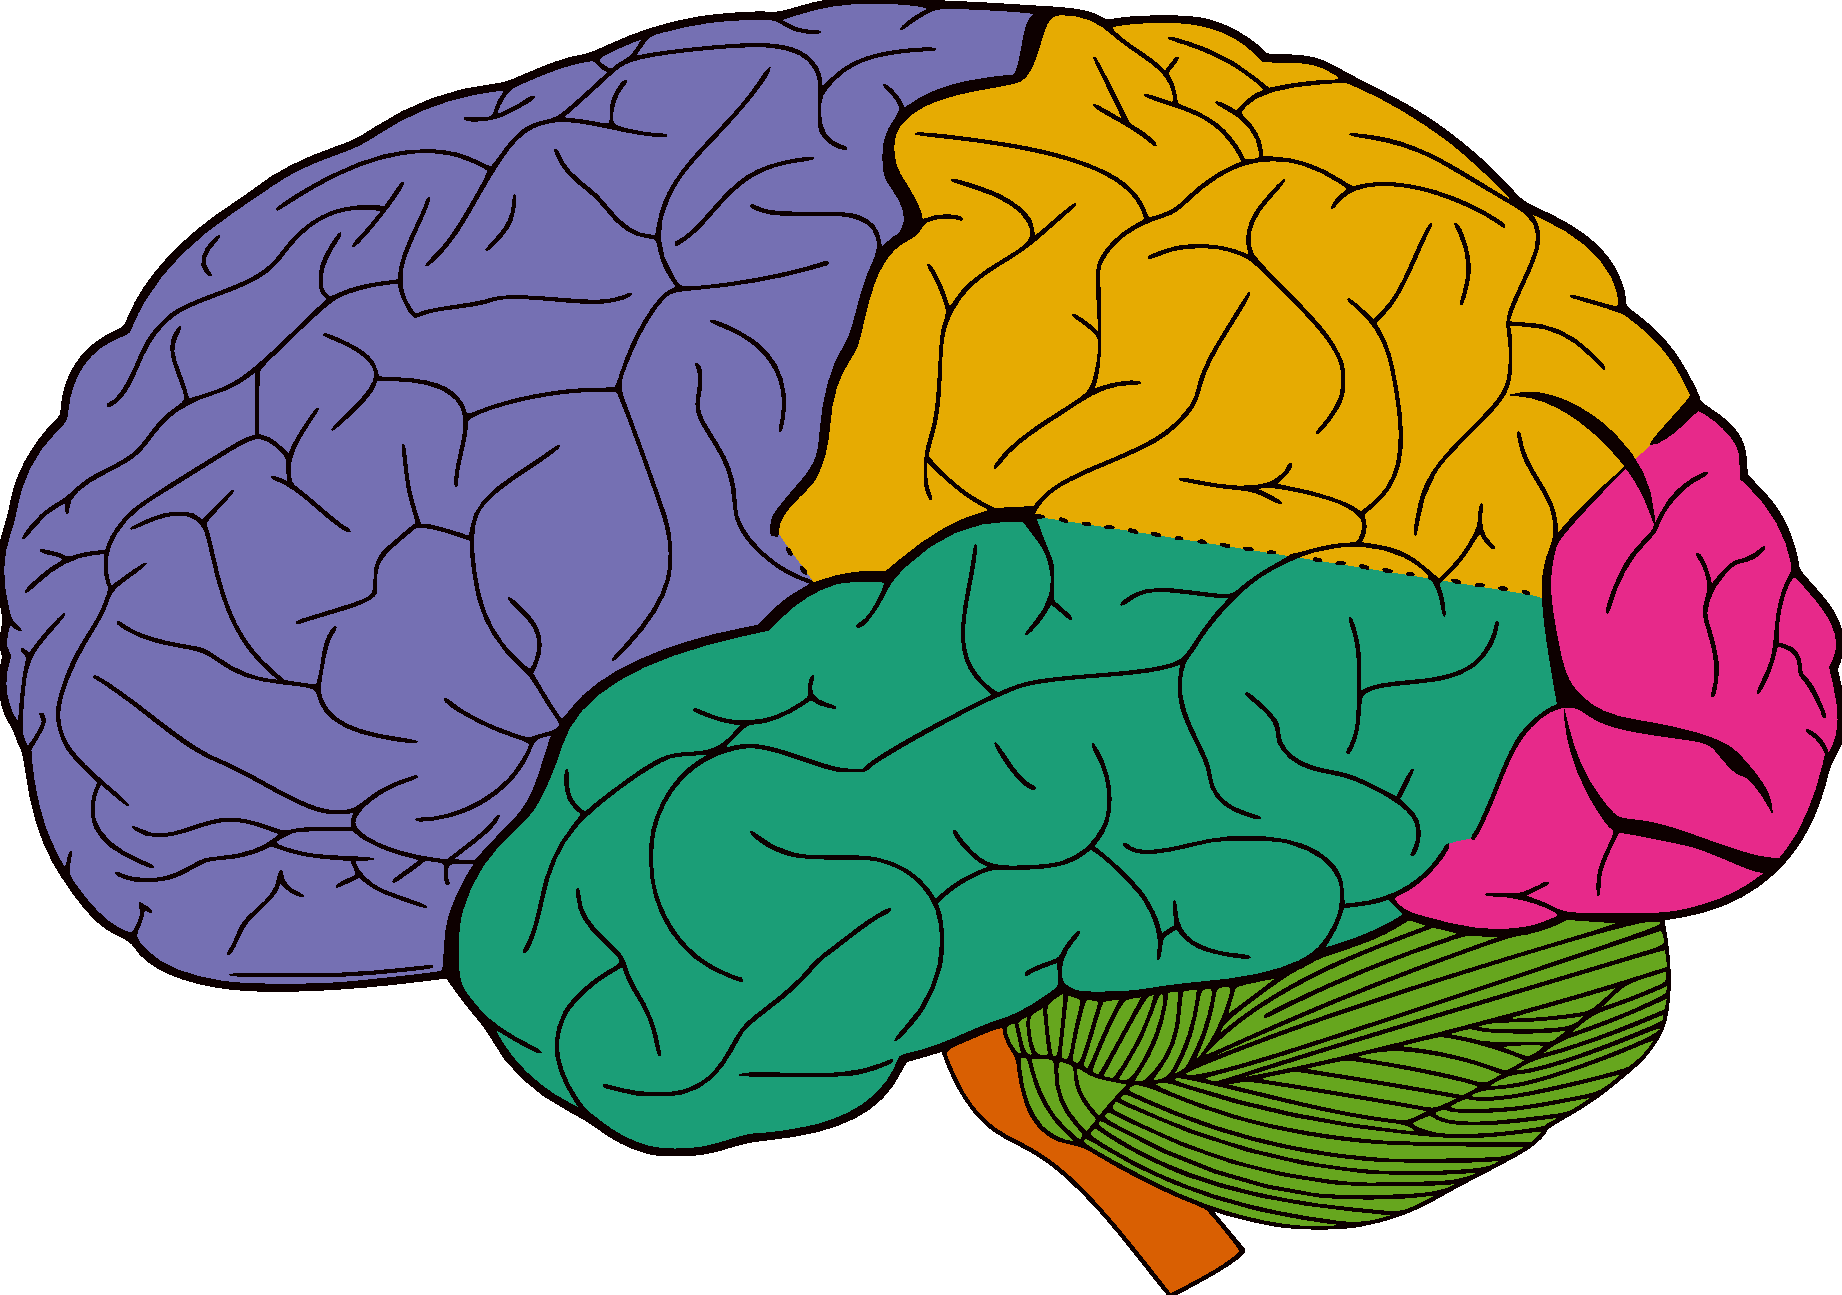
\includegraphics[height=0.3\textwidth]{gfx/neuroanatomy/brain_lobes.pdf}}
\hfill
\tikzset{external/export next=false}
\subcaptionbox{%
        \label{fig:coronalStained}%
        \todo{BB 4201} Coronal section stained for cell bodies. The \ac{GM} is dark while the \ac{WM} is bright. The left and right hemisphere is connected via the corpus calosum.}%
    [0.47\textwidth]{\includegraphics[height=0.3\textwidth]{dev/brain/BB_4201.png}}
    % \begin{tikzpicture}[]
    %     \node[inner sep=0pt, anchor = south west] (fig) at (0,0)
    %     {\includegraphics[height=0.3\textwidth]{dev/brain/BB_4201.png}};
    %     \coordinate (WM1) at ($(fig.north west)!0.6!(fig.north east)$);
    %     \coordinate (WM2) at ($(fig.north east)!0.35!(fig.south east)$);
    %     \draw[RED, ultra thick, <-] (WM1 |- WM2) -- ++ (-42:0.75) node[pos=1, anchor=north] {\textbf{WM}};
    %     \coordinate (GM1) at ($(fig.north west)!0.275!(fig.north east)$);
    %     \coordinate (GM2) at ($(fig.north east)!0.125!(fig.south east)$);
    %     \draw[GREEN, ultra thick, <-] (GM1 |- GM2) -- ++ (-65:0.75) node[pos=1, anchor=north] {\textbf{GM}};
    % \end{tikzpicture}
% }
\caption{Illustration of the human brain and a cell body stained coronal section.}
\label{fig:humanBrain}
\end{figure}
%
The cerebellum and cerebrum contain a \ac{GM} stucture at the brain surface.
This structure is filled with neurons.
These cells have the task of processing the information of all signals coming from inside and outside of the brain.
These cells are arranged in cortical layers that have different thicknesses, cell types, and densities specific to a brain area.
These cells have a relatively high density and are not only locally interconnected with each other, but connect also with different brain areas.
%  (see \cref{fig:nerveFiber,fig:cortLayers}).
Therefore, the folding of the brain is particularly important to increase the surface and therefore the number of cells.
In the human brain there are several billions of nerve cells.
There are many types of cells, \eg{} granule or pyramidal cells.
The highly interconnected structure and arrangement of the various cells is the source of its high number of different functionalities.
It is imporatant to investiagte the human brain to gain a better understanding of the brain's function and an improved understanding of pathophysiological processes that may lead to improved medical treatment of brain deseases.
%
%
%
\section{Fiber architecture} \label{sec:fiberArchitecture}
%
\begin{figure}[!t]
\centering
% \subcaptionbox{
%     \label{fig:cortLayers}
%     Cortical layers \todo{wichtig?}
%     }[0.225\textwidth]{\includegraphics[height=4.5cm]{dev/wiki/layers.png}}
% \hfill
\tikzset{external/export next=false}
% \subcaptionbox{
%     \label{fig:nerveCell}
%     Nerve cell structure.
% }[0.75\textwidth]{
\begin{tikzpicture}[every node/.style={font=\small,},]
    \node[inner sep=0pt, anchor = south west] (fig) at (0,0) {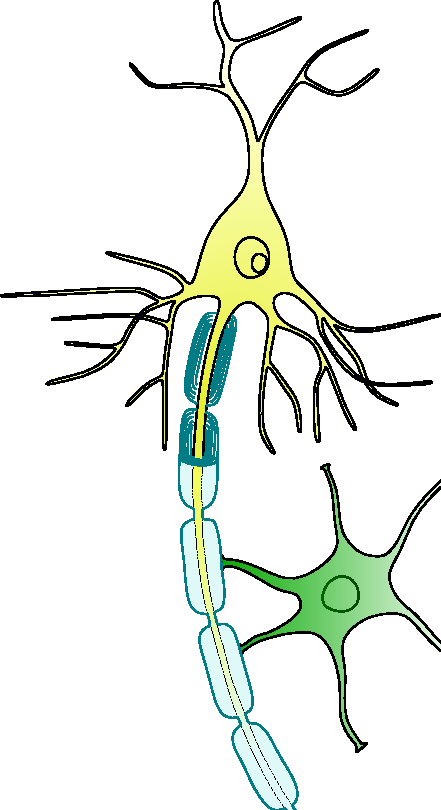
\includegraphics[ angle=90,width=0.75\textwidth]{gfx/neuroanatomy/neuron-axon.pdf}}; %height=4.2cm
    \begin{scope}[overlay]
        % \foreach \p in {0,0.1,0.2,0.3,0.4}{
        %     \draw[blue] (rel cs:name=fig,x=\p,y=\p) rectangle (rel cs:name=fig,x=1-\p,y=1-\p);
        % }
        % 
        \node[anchor=south] at (rel cs:name=fig,x=0.72,y=1.025) {Oligodendrocyte};
        \node[anchor=north] at (rel cs:name=fig,x=0.235,y=0.22) {Cell Body};
        \node[anchor=west] at (rel cs:name=fig,x=1,y=0.675) {Axon};
        \node[anchor=north] at (rel cs:name=fig,x=0.7,y=0.4) {Myelin};
        \draw[<-] (rel cs:name=fig,x=0.9,y=0.5) -- ++(-69:0.5) node[pos=1,anchor=north] {Node of Ranvier};
        \draw[<-] (rel cs:name=fig,x=0.295,y=0.53) -- ++(-140:0.75) node[pos=1,anchor=north] {Nucleus};
        \node[anchor=south] at (rel cs:name=fig,x=0.24,y=0.8) (D) {Dendrites};
        \draw[->] (rel cs:name={D},x=0.3,y=0) -- ++(-155:0.6){};
        \draw[->] (rel cs:name={D},x=0.7,y=0) -- ++(-25:0.6){};
    \end{scope}
    \path[] ($(fig.south west)-(0,0)$) rectangle ($(fig.north east)+(1,0.75)$);
\end{tikzpicture}
% }
\caption{Illustration of a neuron with axon and oligodendrocytes. The olegodendrocyte build up a layered lipid structure up, surrounding the axon. The myelin layers are separated along the axon by nodes of Ranvier.}
\label{fig:CortexAndNerveCell}
\end{figure}
%
Nerve cells are connected by nerve fibers.
A typical nerve cell (see \cref{fig:nerveCell}) comprises a cell body, called a soma, that processes incoming information.
The information arrives via dendrites, which are star-shaped branches.
The axon is the cell's only information output.
It travels through the brain often associated with nerve fiber bundles to its destination, where it connects with the axon terminal to other neurons.
\par
%
The axon is surrounded by a myelin sheath, a lipid layered structure deriving from nearby olegodendrides (see \cref{fig:human-brain}).
The myeling electrically insulates the axon and improves the speed of propagation of the electrical action potential along the axon and also its signal strength.
The diamater of the myelin ranges from about $\SI{0.5}{\micro\meter}$ to several $\si{\micro\meter}$ (see \cref{tag:axonDiameter}).
There are many different types of axons.
Some contain a very thick myelin layer, while others have none.
The high density of axons and myelin makes the brainappear white and is therefore called \ac{WM}, whereas the outer cell bodys appear darker and ist called \ac{GM}.
This color difference is clearly visible in a Nissle stained histological sections (see \cref{fig:coronalStained}).
\par
%
To enhance the contrast of the nerve fibers to the background, staining like Nissle is used to darken the myelin (see \cref{fig:brainMyelinStain}).
This allows to follow small nerve fibers down to individual nerves depending on their myelination degree.
Larger nerve fiber bundles are such dark, that mostly no orientation can be exracted.
\par
% 
\Cref{fig:brainMyelinStain} shows a nissle stained brain section.
% Both single nerve fibers and nerve fiber bundles are visible.
Between neurons, individual nerve fibers form complex reticular structures.
Several nerve fiber bundles trace their paths through the thalamus and are visible as dark structures.
% 
A closer look with an electron microscope into a nerve fiber bundle of the corpus callosum of a rodent is shown in \cref{fig:elecMic}.
The nerve fibers of the $\SI{100}{\nano\meter}$ thin section are densely packed together.
Axon diameter and myelin thickness vary from nerve fiber to nerve fiber.
% 
\begin{figure}[!t]
	\centering
    \tikzset{external/export=false}
    \subcaptionbox{%
        \label{fig:brainMyelinStain}
        Myelin staining of the human thalamus, sagital section. \textcolor{Orange}{Nerve fiber bundle} structures are visiable as as cut structures visible as elliptical dark shape. In between \textcolor{ProcessBlue}{net-like structures} are fromed from individual nerve fibers. \url{http://brainmaps.org/HBP3/h.sapiens/sag/h5thal-myelin/17a}}
    [.49\textwidth]{
        \begin{tikzpicture}[]  
            \node[inner sep=0pt, anchor = south west] (fig) at (0,0)
            {\includegraphics[width=0.49\textwidth, trim=281 152 0 0, clip]{gfx/neuroanatomy/NeuralNet-BrainAtlasDotOrg.png}};
            %  
            \draw[Orange, ultra thick] (rel cs:name=fig,x=0.42,y=0.49) ellipse (0.75 and 0.375);
            \draw[ProcessBlue, ultra thick] (rel cs:name=fig,x=0.7,y=0.3) ellipse (1.1 and 0.7);
            % 
            \draw[white, ultra thick] let
                \p1=(rel cs:name=fig,x=0,y=0), 
                \p2=(rel cs:name=fig,x=0.1041,y=0), 
                \n1={veclen(\x1-\x2,\y1-\y2)}
            in
                ($(fig.south east)+(-0.2,0.2)$) -- ++ (180:\n1) node[above, midway, anchor=south]{$\SI{50}{\micro\meter}$};
        \end{tikzpicture}        
    }
    \hfill
    \subcaptionbox{%
        \label{fig:elecMic} Electron microscope image of a $\SI{100}{\nano\meter}$ thin section of rodent corpus callosum \cite{WALHOVD20142}. The myelin is visible as dark soroundings around the inner axon.}
    [.49\textwidth]{
        \begin{tikzpicture}[]  
            \node[inner sep=0pt, anchor = south west] (fig) at (0,0)
            {\includegraphics[width=0.49\textwidth]{dev/brain/elec_micrograph_rodent_cc.jpg}};
            \draw[white, ultra thick] let
                \p1=(rel cs:name=fig,x=0,y=0), 
                \p2=(rel cs:name=fig,x=0.1347,y=0), 
                \n1={veclen(\x1-\x2,\y1-\y2)}
            in
                ($(fig.south east)+(-0.2,0.2)$) -- ++ (180:\n1) node[above, midway, anchor=south]{$\SI{1}{\micro\meter}$};
        \end{tikzpicture}
    }
\end{figure}
% 
%
%
\section{Axon Literature}
\label{sec:axonMicroscopy}
%
\Cref{tab:axonDiameter} lists the results of the nerve fiber diameter.
The diameter and their standard deviation are region-specific.
The $g_{\mathit{ratio}}$ describes the fraction of the axon to the entire nerve fiber diameter.
From studies with \ac{dMRI} and electron microscopy
\cite{Stikov2015,Dean2016,Mohammadi2015,Cercignani2017,Berman2018,Jung2018} the $g_{\mathit{ratio}}$ is in the range of $\SI{0.6}{}$ to $\SI{0.9}{}$, depending on the region (see \cref{tab:gratio}).
%
\begin{table}[!b]
\centering
\pgfplotstabletypeset[
    thesisTableStyle,
    font=\footnotesize,
    % col sep=comma,
    columns/area/.style={string type},
    columns/mean/.style={string type},
    columns/std/.style={string type},
]{
    area mean std
    {sup. longitudinal fascide} $\SI{0.8}{\micro\meter}$ $\SI{0.2}{\micro\meter}$
    {Unicate/inferior occipital fasc.} $\SI{0.51}{\micro\meter}$ $\SI{0.05}{\micro\meter}$
    {corpus calosum} $\SI{0.69}{\micro\meter}$ $\SI{0.04}{\micro\meter}$
}
\caption{Nerve fiber diameter distribution of the human brain. Mean values over three human brains \cite{Liewald2014}.}
\label{tab:axonDiameter}
\end{table}
%
\begin{table}[!b]
\centering
\pgfplotstabletypeset[
thesisTableStyle,
font=\footnotesize,
col sep=semicolon,
columns={article,cite,gratio},
columns/article/.style={string type, column name=study, column type = {l}},
columns/cite/.style={string type, column name=cite, column type = {l}},
columns/gratio/.style={string type, column name=$g_{\mathit{ratio}}$},
]{data/gratio.csv}
\caption{human $g_{\mathit{ratio}}$ from invivo mri studies.}
\label{tab:gratio}
\end{table}
\setcounter{chapter}{2}
\chapter{Theory}
\label{sec:theory}
% 
\cleanchapterquote{The first principle is that you must not fool yourself and you are the easiest person to fool.}{Richard P. Feynman}{}%\newline
%
\section{Introduction}
The following section lists the physical theories needed to describe the mathematics behind \ac{3D-PLI}. This includes the basic properties of light with the description of their polarization state, the optical models of the tissue, i.e. the nerve fibers and the mathematical description of the experimental setup of \ac{3D-PLI} and the analysis of its signal. The first part of this chapter was written with the help of \cite{demtroeder2, Fliebach2012}.
% 
% 
% 
\section{Electromagnetic Wave}
% 
Light is an electromagnetic wave. Electromagnetism is first fully described by James Clerk Maxwell. He formulated the Maxwell-Equations \cref{eq::maxwell_general}, generalized from the previous work of Johann Carl Friedrich Gau{\ss}, Michael Faraday and Andr\'{e}-Marie Amp\`{e}re and others:
% 
% \begin{align} 
% \begin{split} \label{eq::maxwell_macro}
%     \nabla \cdot \vec{D} &= 4\pi\rho_\text{f}\\
%     \nabla \cdot \vec{B} &= 0\\
%     \nabla \times \vec{E} &= -\frac{1}{c} \frac{\partial \vec{B}} {\partial t}\\
%     \nabla \times \vec{H} &= \frac{1}{c} \left(4\pi\vec{J}_\text{f} + \frac{\partial \vec{D}} {\partial t} \right)
% \end{split}
% \end{align}
% 
\begin{align} 
\begin{split} \label{eq::maxwell_general}
    \nabla \cdot \vec{E} &= \frac {\rho} {\varepsilon_0}\\
    \nabla \cdot \vec{B} &= 0\\
    \nabla \times \vec{E} &= -\frac{\partial \vec{B}} {\partial t}\\
    \nabla \times \vec{B} &= \mu_0\left(\vec{j} + \varepsilon_0 \frac{\partial \vec{E}} {\partial t} \right)
\end{split}
\end{align}
% 
with $\nabla \coloneqq \left({\frac{\partial}{\partial x}}, {\frac{\partial}{\partial y}}, {\frac{\partial}{\partial z}} \right)$ as vector differential operator, $\vec{E}$ as eletric field, $\rho$ as electric charge density, $\varepsilon_0$ as permittivity of free space, $\vec{B}$ as magnetic field, $\mu_0$ as permeability of free space and $\vec{j}$ as electric current density.
% 
The first equation states no electric field can be generated without an electric charge (charge conservation).
The second equation states, magnetic monopoles does not exists. The basic entity of an magnetic field is a dipole.
The third and forth equation show the interconnection of the electric and magnetic fields in space and time.
A change in the electric field yields to a magnetic field and vice versa.
Equation forth additional indicates the creation of a magnetic field from a electric current $\vec{j}$.
The maxwell equation fullfill the continoiut ... $\divergence j + \frac{\partial \rho}{\partial t} = 0$.
This means that neither an electric of magnetc field can be created without either an electric current or a change of electric potential.
%
% \par
% 
\subsection{EM in a vacuum}
% 
In a vacuum this simplifies with $\rho = 0$ and $\vec{j} = \vec{0}$ to:
% 
\begin{align}
\begin{split} \label{eq::maxwell_vacuum}
  \nabla \cdot \vec{E} &= 0 \quad\\
  \nabla \cdot \vec{B} &= 0 \quad\\
  \nabla \times \vec{E} &= -\frac{\partial\vec B}{\partial t}\\
  \nabla \times \vec{B} &= \mu_0\varepsilon_0 \frac{\partial\vec E}{\partial t}
  \end{split}
\end{align}
% 
With 
\begin{align}
\begin{split} 
    \nabla \times \nabla \times \vec{E} = -\nabla \times \frac{\partial \vec{B}} {\partial t} &= -\frac{\partial} {\partial t} \left( \nabla \times  \vec{B} \right)\\
    &= -\varepsilon_0 \cdot \mu_0 \frac{\partial^2 \vec{E}}{\partial t^2} \, ,
\end{split}
\end{align}
% 
the identity $\nabla \times \left( \nabla \times \vec{A} \right) = \nabla(\nabla \cdot \vec{A}) - \nabla^{2}\vec{A}$ and $\mu_0\varepsilon_0 = \frac{1}{c^2}$, with $c$ as the speed of light\footnote{can be derived from Maxwells equation and Lorentz force in a vacuum}, this further simplifies to:
% 
\begin{align}
\begin{split} \label[pluralequation]{eq::maxwell_wave_equations}
  \frac{1}{c^2} \frac{\partial^2 \vec{E}}{\partial t^2} - \nabla^2 \vec{E} &= 0 \\
  \frac{1}{c^2} \frac{\partial^2 \vec{B}}{\partial t^2} - \nabla^2 \vec{B} &= 0
\end{split}
\end{align}
% 
% Another common representation is
% % 
% \begin{align}
% \begin{split} \label{eq::maxwell_wave_equations_box}
%   \Box \ \vec{E} &= 0 \\
%   \Box \ \vec{B} &= 0
% \end{split}
% \end{align}
% 
% with the help of the d'Alembert operator $\Box \coloneqq \partial^a\partial_a = \nabla^2 - \frac{1}{c^2} \frac{\partial^2}{\partial t^2}$.
% 
This also shows that $c^2  \frac{\partial B} {\partial z} = \frac{\partial E}{\partial t} \Rightarrow \vec{E} \cdot \vec{B} = 0$ and therefore the electric and magnetic field components are perpendicular to each other.
Additionally it also means, that space and time are interconnected and that light travels in vacuum with the speed of light $c$.
% 
\subsection{Solving MW Equ in vacuum}
% 
\Cref{eq::maxwell_wave_equations} have the shape of a wave equation and can therefore as known be solved by
% 
% Using the Maxwell equation in vacuum \ref{eq::maxwell_vacuum}, one can find the most simple solution to the differential equation is a wave:
% 
\begin{align}
\begin{split} \label{eq::dgl_solution}
  \vec{E}( \vec{r}, t ) &= g(\phi( \vec{r}, t )) = g( \omega t - \vec{k} \cdot \vec{r} + \varphi)\\
  \vec{B}( \vec{r}, t ) &= g(\phi( \vec{r}, t )) = g( \omega t - \vec{k} \cdot \vec{r} + \varphi )
\end{split}
\end{align}
% 
where $g$ is any well behaved function (continuous and differentiable) and therefore also their superposition.
% 
With the help of
% 
\begin{align}
k = \mathopen| \vec{k} \mathclose| = \frac{\omega}{c} =  \frac{2 \pi}{\lambda}
\end{align}
% 
a planar wave can be descriped by
% 
\begin{align}
\begin{split} \label{eq::plane_wave}
\vec{E}(\vec{r}) &= \vec{E}_0 \cdot e^{ -i \, \vec{k} \cdot \vec{r} }\\
 \vec{B}(\vec{r}) &= \vec{B}_0 \cdot e^{ -i \, \vec{k} \cdot \vec{r} }
\end{split}
\end{align}
% 
with $\vec{k}$ as Wave vector pointing into the travel direction of the light wave.
% 
% 
\subsection{Polarization}
% 
\begin{figure}[!t]
\centering
\setlength{\tikzwidth}{\textwidth}
\inputtikz{gfx/pli/polarization_state}
\label{fig:polarization_state}
\caption{Illustration of light polarization state. Unpolarized light goes throug a linear polarizer which polarizes the light in one direction (w.l.o.g. $E_x$ and $E_y$ in phase). Afterwords it travels though a quarter wave retarder, which turn linear polarized light (of a specific wave length) into circular polarized light, where w.l.o.g. $E_x$ and $E_y$ are $\pi/2$ phase}
\end{figure}
% 
Since the light wave travels into one direction, and the electric field and magnetic field are perpendicular to $\vec{k}$ as well to each other, there orientation is a fundamental property of light called polarization.
Without any additional info, the polarization orientation is conventional in the direction of the electric field component.
% 
A superposition of x and y wave with z equal to direction of propagation yield w.l.o.g. to the general form
\begin{align}
\vec{E}(z,t) &= \begin{pmatrix} E_{0x} \cdot e^{ -i \phi_x } \\ E_{0y} \cdot e^{ -i \phi_y } \\ 0 \end{pmatrix}
e^{ -i (kz - \omega t)}
\end{align}
%
\begin{figure}[!t]
\centering
\tikzset{external/export=false}
%
% \captionsetup[sub]{textfont=normalsize}
% \captionsetup[sub]{position=top, skip=-14pt}
\tikzset{cross/.pic={
\draw[arrows={-Latex[scale=1]}] (-{sqrt(2)},0) -- ({sqrt(2)},0) node[anchor=north]{\small $E_x$};
\draw[arrows={-Latex[scale=1]}] (0,-{sqrt(2)}) -- (0,{sqrt(2)}) node[anchor=east]{\small $E_y$};
}}
%
% \subcaptionbox{}[.3\textwidth]{
\begin{tikzpicture}
\begin{scope}[shift={(0,0)}, local bounding box=A]
\pic at (0,0) {cross};
% \draw[] (0, 2) node[font=\small] () {linear, horizontal};
\draw[very thick, arrows={Latex[scale=1]-Latex[scale=1]}] (-1, 0) -- (1, 0);
\draw[] (0, -2) node () {$\begin{pmatrix} 1&0 \end{pmatrix}$};
\draw[] (0, -2.75) node () {$\begin{pmatrix} 1&1&0&0 \end{pmatrix}$};
\end{scope}
\node[anchor=south west, xshift=-1em] at (A.north west) {\small \textcolor{magenta}{\textbf{(a)}} linear, horizontal};
% }\hfill
% \subcaptionbox{}[.3\textwidth]{
\begin{scope}[shift={(4,0)}, local bounding box=B]
\pic at (0,0) {cross};
% \draw[] (0, 2) node[font=\small] () {linear, vertical};
\draw[very thick, arrows={Latex[scale=1]-Latex[scale=1]}] (0, -1) -- (0, 1);
\draw[] (0, -2) node () {$\begin{pmatrix} 0&1 \end{pmatrix}$};
\draw[] (0, -2.75) node () {$\begin{pmatrix} 1&-1&0&0 \end{pmatrix}$};
\end{scope}
\node[anchor=south west, xshift=-1em] at (B.north west) {\small \textcolor{magenta}{\textbf{(b)}} linear, vertical};
% }\hfill
% \subcaptionbox{}[.3\textwidth]{
\begin{scope}[shift={(8,0)}, local bounding box=C]
\pic at (0,0) {cross};
% \draw[] (0, 2) node[font=\small] () {linear, $\pi/4$};
\draw[very thick, arrows={Latex[scale=1]-Latex[scale=1]}] (-1, -1) -- (1, 1);
\draw[] (0, -2) node () {$\begin{pmatrix} 1&1 \end{pmatrix}$};
\draw[] (0, -2.75) node () {$\begin{pmatrix} 1&0&1&0 \end{pmatrix}$};
\begin{scope}[overlay]
\draw[] (2, -2) node () {Jones};
\draw[] (2, -2.75) node () {Stokes};
\end{scope}
\end{scope}
\node[anchor=south west, xshift=-1em] at (C.north west) {\small \textcolor{magenta}{\textbf{(c)}} linear, $\pi/4$};
% }
% \\[2em]
% \subcaptionbox{}[.32\textwidth]{
\begin{scope}[shift={(0,-5.75)}, local bounding box=D]
\pic at (0,0) {cross};
% \draw[] (0, 2) node[font=\small] () {left circular};
\draw[very thick] plot[domain=0:360,samples=90,smooth] ({cos(\x)},{sin(\x)});
\draw[very thick, arrows={-Latex[scale=1]}] plot[domain=44:45,samples=1] ({cos(\x)},{sin(\x)});
\draw[very thick, arrows={-Latex[scale=1]}] plot[domain=224:225,samples=1] ({cos(\x)},{sin(\x)});
\draw[] (0, -2) node () {$\begin{pmatrix} 1&i \end{pmatrix}$};
\draw[] (0, -2.75) node () {$\begin{pmatrix} 1&0&0&-1 \end{pmatrix}$};
\end{scope}
\node[anchor=south west, xshift=-1em] at (D.north west) {\small \textcolor{magenta}{\textbf{(d)}} left circular};
% }\hfill
% \subcaptionbox{}[.32\textwidth]{
\begin{scope}[shift={(4,-5.75)}, local bounding box=E]
\pic at (0,0) {cross};
% \draw[] (0, 2) node[font=\small] () {right circular};
\draw[very thick] plot[domain=0:360,samples=90,smooth] ({cos(\x)},{sin(\x)});
\draw[very thick, arrows={-Latex[scale=1]}] plot[domain=46:45,samples=1] ({cos(\x)},{sin(\x)});
\draw[very thick, arrows={-Latex[scale=1]}] plot[domain=226:225,samples=1] ({cos(\x)},{sin(\x)});
\draw[] (0, -2) node () {$\begin{pmatrix} 1&-i \end{pmatrix}$};
\draw[] (0, -2.75) node () {$\begin{pmatrix} 1&0&0&1 \end{pmatrix}$};
\end{scope}
\node[anchor=south west, xshift=-1em] at (E.north west) {\small \textcolor{magenta}{\textbf{(e)}} right circular};
% }\hfill
% \subcaptionbox{}[.32\textwidth]{
\begin{scope}[shift={(8,-5.75)}, local bounding box=F]
\pic at (0,0) {cross};
% \draw[] (0, 2) node[font=\small] () {unpolarized};
\draw[] (0, -2.75) node () {$\begin{pmatrix} 1&0&0&0 \end{pmatrix}$};
\begin{scope}[overlay]
\draw[] (2, -2) node () {Jones};
\draw[] (2, -2.75) node () {Stokes};
\end{scope}
\end{scope}
\node[anchor=south west, xshift=-1em] at (F.north west) {\small \textcolor{magenta}{\textbf{(f)}} unpolarized};
%
\path[] ($(A.west)!-0.075!(C.east)$) -- ($(A.west)!1.075!(C.east)$);
\end{tikzpicture}
% }
%
\caption{polarization states, check vector length,\itodo{test speed}} 
\label{fig:polarization_state_vectors}
\end{figure}
%
\Cref{fig:polarization_state_vectors} shows another representation of the polarization sate of a light wave.
It show the component perpendicular to the travelling direction.
Therefore the time variation can be shown on the xy-plane.
Additionally the states can be describe by the Jones or Stokes calculus, later described in \cref{sec:jones,sec:mueller_stokes}.
% 
% 
% 
\subsection{Light in medium}
% 
The Maxwell equations in \dummy{} are described above. They can be solved analog to \dummy{}. This yields to some special behavior, \eg{} the magnetic and electric field component get out of phase.
However here only the two properties of absorption and diffraction are described.
They derivation can be found \eg{} \cite{demtroeder2, Fliebach2012}.
% 
\subsection{Absorption}
% 
\begin{align}
    I = I_0 \exp(-\mu x)
\end{align}
\todo{herleiten}
% 
Beersche law of absorption with $\mu = \frac{4\pi \kappa}{\lambda_0}$ where $\kappa$ is the imaginary part of the complex refractive index.
% 
\subsection{Refraction}
% 
\begin{figure}[!t]
\centering
\setlength{\tikzwidth}{\textwidth}
\inputtikz{gfx/pli/refraction}
\label{fig:optic_refraction}
\caption{Illustration of refraction.}
\end{figure}
% 
Refraction is the property of light to change direction as it passes from one medium to another. This can be shown by using the full Maxwell equations  for non-conductive material, \ie{} $\vec{j} = 0, \rho = 0$, that the differential equating consist out of a primary wave with from atomic medium induced secondary waves, which leads to a reduction of the velocity of the resulting wave. Mathematically this can be described by a complex number $n = c' / c$.
Using this relationship at a boundary surface between two media, one can show that the incident light beam splits into a reflecting and transmitting light wave. The reflecting light wave has the same angle as the incident light beam relative the the surface normal. The transmitting light beam however due to the reduction of the velocity, changes its direction described by the Snellius law
\begin{align}
    n_0 \sin \alpha = n_1 \sin \beta
\end{align}

% 
\begin{align}
\underline{n} = n + i\kappa
\end{align}
% 
\begin{align}
\begin{split}
\vec{E}(z, t) &= \operatorname{Re}\! \left[\vec{E}_0 \cdot e^{i\, (kz - \omega t)}\right] \\
&= \operatorname{Re}\! \left[\vec{E}_0 \cdot e^{i\, (2\pi(n + i\kappa)z/\lambda_0 - \omega t)}\right] \\
&= e^{-2\pi \kappa z/\lambda_0} \operatorname{Re}\! \left[\vec{E}_0 \cdot e^{i\, (kz - \omega t)}\right]
\end{split}
\end{align}\todo{?}
% 
% 
% 
\subsection{Birefingence}
%
\begin{figure}[!t]
\centering
\setlength{\tikzwidth}{\textwidth}
\inputtikz{gfx/pli/retardation}
\caption{Illustration of retardation.}
\label{fig:optic_retardation}
\end{figure}
% 
\begin{figure}[!t]
\centering
\subcaptionbox{}[.49\textwidth]{
\setlength{\tikzwidth}{0.49\textwidth}
\inputtikz{gfx/pli/ellipsoid_a}}
\subcaptionbox{}[.49\textwidth]{
\setlength{\tikzwidth}{0.49\textwidth}
\inputtikz{gfx/pli/ellipsoid_b}}
\caption{birefringence elipsoid}
\label{fig:index_elipsoid}
\end{figure}
% 
Material can have a different refractive index depending on the relative orientation and polarization of the light beam.
This property is known as birefringence.
The refractive index can be described as the refractive index $n_o$ and extraordinary  $n_e$.
Since these two are perpendicular to each other, one can split the light beam into the same perpendicular parts and describe each by its own.
These two light beams, except for the trivial case of a light beam is perpendicular to the surfave, have a different direction.
However for small relative length (hängt von n ab, bzw der phasenänderung) the two light beams leave the material at the same point and recombined at the end.
The change of phase is called birefringence and is described by the difference between the .. and ...
% 
\begin{align}
    \Delta n = n_e - n_o \> .
\end{align}
% 
This .. can be visualized by the index ellipsoid \cref{fig:index_elipsoid}.
The change of the amplitude and phase can be described by the following two vector matrices descriptions.
% 
% 
% 
\subsection{Jones calculus}
\label{sec:jones}
% 
The Jones calculus, introduced by Robert Clark Jones in 1941, describes the polarization state of a light beam by a complex vector $J$:
% 
\begin{align}
    \vec{J} = \begin{pmatrix} E_x \exp(i \phi_x) \\ E_y \exp(i \phi_y) \end{pmatrix}
\end{align}
% 
The amplitude of the perpendicular components are $E_x$ and $E_y$ with their phase $\phi_x$ and $\phi_y$.
Optical elements, which changes the polarization state, such as a polarization filter and retarder, can be desribed by a matrix:
% 
\begin{align}
\begin{split}
\mat{P}_x = 
\begin{pmatrix}
1 & 0 \\ 0 & 0
\end{pmatrix}
, \,
\mat{P}_y = 
\begin{pmatrix}
0 & 0 \\ 0 & 1
\end{pmatrix}
, \,
\mat{M} =
\begin{pmatrix}
e^{i \varphi_x} & 0 \\ 0 & e^{i \varphi_y}
\end{pmatrix}
, \,
\Lambda_{1/4}=
e^{\frac{i \pi}{4}}
\begin{pmatrix}
1 & 0 \\ 0 & -i
\end{pmatrix}
\end{split}
\end{align}
% 
A rotation of an optical element can be achieved by a 2d rotation matrix $\mat{R}$:
% 
\begin{align}
\begin{split}
\mat{M}(\theta )=\mat{R}(\theta )\cdot\mat{M}\cdot\mat{R}(-\theta )
, \>
\mat{R}(\theta ) = 
\begin{pmatrix}
\cos \theta & -\sin \theta \\
\sin \theta & \cos \theta
\end{pmatrix}
\end{split}
\end{align}
% 
% 
% 
\subsection{M\"uller-Stokes}\label{sec:Mueller-Stokes}
\label{sec:mueller_stokes}
% 
Analog to \cref{sec:jones} the M\"uller-Stokes formalism, described by George Gabriel Stokes in 1852, also describes the polarization state (how good is it \dummy{}) of a light beam.
However it does not use the absolute .. but the relative polarization between both components:
% 
\paragraph{Stokes vector}
\begin{align}
\begin{split}
S_0 &= I \\
S_1 &= I p \cos 2\psi \cos 2\chi \\
S_2 &= I p \sin 2\psi \cos 2\chi \\
S_3 &= I p \sin 2\chi
\end{split} \hspace{-6em}
\begin{split}
& \equiv \langle E_x^{2} \rangle + \langle E_y^{2} \rangle \\
%  & = \langle E_a^{2} \rangle + \langle E_b^{2} \rangle \\
%  & =  \langle E_l^{2} \rangle + \langle E_r^{2} \rangle \\
& \equiv \langle E_x^{2} \rangle - \langle E_y^{2} \rangle \\
& \equiv \langle E_a^{2} \rangle - \langle E_b^{2} \rangle \\
& \equiv  \langle E_l^{2} \rangle - \langle E_r^{2} \rangle
\end{split}
, \,
\vec{S} =
\begin{pmatrix} S_0 \\ S_1 \\ S_2 \\ S_3\end{pmatrix}
\end{align}
% 
% \begin{align}
% \begin{split}
% S_0 & \equiv \langle E_x^{2} \rangle + \langle E_y^{2} \rangle \\
%  & = \langle E_a^{2} \rangle + \langle E_b^{2} \rangle \\
%  & =  \langle E_l^{2} \rangle + \langle E_r^{2} \rangle \\
% S_1 & \equiv \langle E_x^{2} \rangle - \langle E_y^{2} \rangle \\
% S_2 & \equiv \langle E_a^{2} \rangle - \langle E_b^{2} \rangle \\
% S_3 & \equiv  \langle E_l^{2} \rangle - \langle E_r^{2} \rangle
% \end{split}
% \end{align}
% 
Therefore the phase can not be described anymore.
However the relative phase information is stored and can be used to describe also polarization states of polarization filters, which can not be described by Jones.
Aanlog to Jones one can formulate the matrices for the optical components:
% 
\paragraph{Linear Polarizer}
\begin{align}
\mat{P}_x=\frac{1}{2}
\begin{pmatrix}
    1 & 1 & 0 & 0 \\
    1 & 1 & 0 & 0 \\
    0 & 0 & 0 & 0 \\
    0 & 0 & 0 & 0
  \end{pmatrix}
, \,
\mat{P}_y=\frac{1}{2}
\begin{pmatrix}
     1 & -1 & 0 & 0 \\
    -1 &  1 & 0 & 0 \\
     0 &  0 & 0 & 0 \\
     0 &  0 & 0 & 0
\end{pmatrix}
\end{align}
% 
\paragraph{retarder}
\begin{align}
\mat{M}=\
\begin{pmatrix}
    1 & 0 & 0 &  0 \\
    0 & 1 & 0 &  0 \\
    0 & 0 & \cos \delta & \sin \delta \\
    0 & 0 & -\sin \delta &  \cos \delta
\end{pmatrix}
\end{align}
% 
\paragraph{Quarter-wave plate (fast-axis vertical)}
\begin{align}
\Lambda_{1/4}=\
\begin{pmatrix}
    1 & 0 & 0 &  0 \\
    0 & 1 & 0 &  0 \\
    0 & 0 & 0 & -1 \\
    0 & 0 & 1 &  0
\end{pmatrix}
\end{align}
% 
\paragraph{Rotation Matrix}
\begin{align}
\mat{R}(\theta)=
\begin{split}
\begin{pmatrix}
    1 &                0 &               0 & 0 \\
    0 & \cos{(2\theta)} & -\sin{(2\theta)} & 0 \\
    0 & \sin{(2\theta)} & \cos{(2\theta)} & 0 \\
    0 &                0 &               0 & 1
  \end{pmatrix}
\end{split}
\end{align}
% 
Analog to \dummy{} rotations are applied by
\begin{align}
\mat{M}(\theta )=\mat{R}(\theta )\cdot\mat{M}\cdot\mat{R}(-\theta )
\end{align}
% 
% \section{Tissue Discretization}
% % 
% By deviding the volume into small diskreticed subvolumes, one can multiply the .. all together and ... (analog Riemann sum)
% \begin{align}
%     \int F \, dt \approx \sum_n F \, \Delta t
% \end{align}
% see simulation?
% 
%  see simulation
% \paragraph{Micro vs Macro:}
% % 
% % \begin{align}
% %   \int_{y_\textit{min}}^{y_\textit{max}} \vec{v}(y) \,dy\\
% %   x = const
% %   y = y(\alpha,x) = tan(\alpha) \cdot x\\
% %   \vec{v}_r = \begin{pmatrix} \cos(\alpha)\\ \sin(\alpha)\\0\end{pmatrix}, \, \vec{v}_p = \begin{pmatrix} 0\\ 0\\1\end{pmatrix}\\
% %   \vec{v}_r = \begin{pmatrix} \cos(\arctan(y/x))\\ \sin(\arctan(y/x))\\0\end{pmatrix}\\
% %   \int_{y_\textit{min}}^{y_\textit{max}} \vec{v}_p(y) \,dy = (y_\textit{max} - y_\textit{min}) \cdot e_z\\
% %   \int_{y_\textit{min}}^{y_\textit{max}} \vec{v}_r(y) \,dy = \int_{y_\textit{min}}^{y_\textit{max}} \cos(\arctan(y/x)) dy \cdot e_x \\
% %   = x\left(\sinh^{-1}(y_\textit{max}/x) - \sinh^{-1}(y_\textit{min}/x)\right) \\
% %   = 2x \left(\sinh^{-1}\left(\frac{2\sqrt{R-x^2}}{x}\right)\right)
% % \end{align}
% % 
% % \begin{align}
% %     % \frac{\oint \vec{v}_z \mathrm{d}A}{\oint \vec{v}_x \mathrm{d}A} = 
% %     % \frac{\int_{-1}^{1}\abs{\vec{v}} \mathrm{d}x}{\int_{-\frac{\pi}{2}}^{\frac{\pi}{2}} \abs{\vec{v}} \cos(\varphi) \mathrm{d}\varphi} =
% %     % \frac{2}{1}
% %     \frac{A_{\Box}}{A_{\circ}} = \frac{4}{\pi}
% % \end{align}
% % 
% \todo{why 2*dn?}
% 
\section{Experimental Setup}\label{sec:expSetup}
%
\begin{figure}[!t]
    \captionsetup[sub]{position=top}
    \setlength{\tikzwidth}{\textwidth}
	\centering
% 	\subcaptionbox{\label{setup-lap} \ac{LAP}}[\textwidth]{
% % 		\resizebox{0.95\textwidth}{!}{
% 		\inputtikz{gfx/pli/pli_setup}
% % 	}
% 	}\\
% 	\subcaptionbox{\label{setup-pm} \ac{PM}}[\textwidth]{
% % 		\resizebox{0.95\textwidth}{!}{
		\inputtikz{gfx/pli/pli_setup_pm}
% % 	}
% 	}
	\caption{Illustration of PLI setup.}
	\label{fig:pli_setup}
\end{figure}
%
% \begin{figure}[!t]
%     % \captionsetup[sub]{position=top}
%     \setlength{\tikzwidth}{0.3\textwidth}
% 	\centering
% 	\subcaptionbox{\ac{LAP}}[.45\textwidth]{\hfill
% 			\inputtikz{gfx/pli/pli_detail}\hfill}\hfill
% 	\subcaptionbox{\ac{PM}}[.45\textwidth]{\hfill
% 			\inputtikz{gfx/pli/pli_detail_pm}\hfill}
% 	\caption{Illustration of \acs{3D-PLI} setup.}
% 	\label{fig:pli_detail}
% \end{figure}
%
The \ac{3D-PLI} setup is described in \cite{Axer2011} with the tiltable light beam microscope (LMP) in \cite{Wiese:887678}.
For the routine measurements two (three) microscope systems are currently in use.
The first use of a high throughput microscope is the \ac{LAP} with a pixel size of about \SI{60}{\micro\meter}.\footnote{can be change by the optic also to $\SI{40}{\micro\meter}$ and $\SI{20}{\micro\meter}$, but remains for the routine measurements with $\SI{60}{\micro\meter}$.}
It consist out of a led light source (\SI{525}{\nano\meter}), a rotatable polarization filter, a rotatable quarter wave retarder, the specimen stage, which can be tilted for oblique views, a rotatable polarizer.
Both polarizer and quarter wave retarder are rotated at the same time.
The both polarizers have a phase offset of $\SI{90}{\degree}$, the first polarizer and the quarter wave retarder of $\SI{45}{\degree}$ (see (see \cref{setup-lap}).
The second system \ac{LMP3D} microscope fullfills the same measurments, however the retarder is placed after the tissue specimen and fixed with the polarizer without any rotations (see \cref{setup-pm}).
Mathematically it measures the same signal.
\footnote{The rotatable filters of the \ac{LAP} has the advantage, that noise like dust particles can be easy identified and removed. Since the microscop is in a more confined "box" this is not necesarry.}
A difference is that the optical path is in reverse to the \ac{LAP} system.
Since there is a mirror in the path, the image is flipped again so that the coordinate systems stays the same (see \cref{fig:pli_detail}).
% 
\subsection{Signal}
% 
From the M\"{u}ller Matrices (\cref{sec:Mueller-Stokes}) as shown in \cite{MenzelMaster,MenzelDissertation}, that the intensity signal, measured by the \ac{CCD}-sensor, follows a sinusiodal curve:
% 
% \begin{align}
% I = \underbrace{\frac{I_0}{2}}_{\mathclap{\mathit{transmittance}}}
%     \bigl[ \sin\bigl(2\rho - 2{\underbrace{\vphantom{\frac{I_0}{2}} \varphi}_{\mathclap{\mathit{direction}}}} \bigr)
%     \cdot \sin \bigl( {\underbrace{\vphantom{\frac{I_0}{2}} 2\pi\frac{d \dn}{\lambda} \cos^2\left( \alpha \right)}_{\mathclap{\delta \, \coloneqq \, \mathit{retardation}}}} \bigr) \bigr]
% \end{align}
\begin{align}
\label{eq:pli_signal}
\begin{split}
I(\rho, \varphi, \alpha, d) =\frac{I_0}{2}\bigl[ \sin\bigl(2\rho - 2\varphi \bigr)\cdot \sin \bigl( 2\pi\frac{d \dn}{\lambda} \cos^2\left( \alpha \right) \bigr) \bigr] \\
\text{with} \enspace \delta \coloneqq 2\pi\frac{d \dn}{\lambda} \cos^2\left( \alpha \right) \enspace 
\text{and} \enspace \trel \coloneqq \frac{d \dn}{\lambda}
\end{split}
\end{align}
% 
Since \cref{eq:pli_signal} describes a sinosoidal signal, the fourier analysis is a obvious choise.
For a discrete, aquidistant measurement of the rotation angles $\rho$, one can use the fourier series with the three coefficients to describe the signal:
% 
% \begin{align}
% \begin{split}
% A \sin(\omega t + \alpha) + B \sin(\omega t + \beta) &= \sqrt{C^2 + D^2} \cdot \sin \, \left( \omega t + \tan^{-1} \left( \frac{D}{C} \right) \right)
% \end{split}
% \\
% \begin{split}
% C &= A \cos(\alpha)+ B \cos(\beta)\\
% D &= A \sin(\alpha)+ B \sin(\beta)
% \end{split} \nonumber 
% \end{align}

\begin{align}
\begin{split}
\rho &= [\SI{0}{\degree}, \frac{1\cdot180}{N+1}\si{\degree}, \frac{2\cdot180}{N+1}\si{\degree}, ..., \frac{N\cdot180}{N+1}\si{\degree}]\\
a_0 &= \frac{1}{N} \sum(\mathit{data})\\
a_1 &= \frac{2}{N} \sum(\mathit{data} \cdot \sin(2 \cdot \rho)\\
b_1 &= \frac{2}{N} \sum(\mathit{data} \cdot \cos(2 \cdot \rho)
\end{split}
\end{align}

With these the final \ac{3D-PLI} modalities are calculated:

\begin{align}
\begin{split}
\mathit{transmittance} &= 2 \cdot a_0\\
\mathit{direction} &= 0.5 \cdot \atantwo(-b_1 / a_1)\\
\mathit{retardation} &= \frac{\sqrt{a_1^2 + b_1^2}}{a_0}
\end{split}
\end{align}
% 
\itodo{Section Images}
% 
% 
% 
\subsection{Inclination analysis}
% 
To be able to analyse the inclination $\alpha$ one has to distinguish the relative strength of the birefringence from the $\cos^2(\alpha)$.
For this purpose a tiltable specimen was developed, which allows measuring the light signal through the tissue with a different angle of incidence.
This mean, that tissue and therefore the nerve fibers also change their orientation by the tilting angles $\theta, \varphi$.
Additionally the distance the light travels through the tissue, elongates by $1/\cos(\theta)$ \cref{fig:tilted_side_view}.
% 
Depending on the \pixelsize{}, this light travels though the same volume, but with another orientation.
Therefore a measurement of multiple light paths can be ... and the resulting signals can be used to analyse the inclination and relative birefrigente tissue thickness \trel{}.
The angle of incidence on the glass ... and the tissue also changes the angle of the light by Snellius law.
All angles mention here are if not specified always the change of angle of the light inside the tissue (see \cref{fig:tilting_camera_view}). 
This also leads to a perspective shift, which has to be corrected by a registration process.
In this case an affine transformation.
This effect is however neglected in the simulation, since it only adds a parallel offset.
% 
In \cite{Schmitz2018} this analysis published under the name of \ac{ROFL}, which builds up on the work of \cite{Wiese:887678}.
The idea is to fit the measured signals of all light paths simultaniously.
Because the change of signal is proportional to the $\cos(\alpha)$ this however means, that for steep fibers, the changes are not only small, but also the amplitude of the signal is very small.
This leads to the problem of increasing uncertanty with increasing inclination angle.
\\
A further problem is that for a smaller \pixelsize{} the light path cannot be neglected anymore.
For the \ac{LMP3D} system this means, that with a maximal tilting angle of about $\SI{3.9}{\degree}$ and a usually tissue thickness of $\SI{60}{\micro\meter}$ the light path is measured in n \dummy{} pixels away from the non tilting case, if the rotation point is in the center of the tissue.
\\
For homogeneous tissue regions like parts in the dense \ac{WM}, this can be ignored.
For single fiber paths in the \ac{GM} however this is currently an unsolved problem.
% 
% 
% 
\section{Orientation visualization}
% 
\begin{figure}[!t]
\centering
\setlength{\tikzwidth}{0.4\textwidth}
\begin{center}
\begin{tabular}{m{6cm}m{6cm}}
\includegraphics[width=\tikzwidth]{gfx/pli/color_sphere.png}
&
\inputtikz{gfx/pli/hsv_sphere}
\\
\begin{minipage}[t]{0.42\textwidth}
\leavevmode\subcaption{2d hsv sphere}
\end{minipage}
&
\begin{minipage}[t]{0.42\textwidth}
\leavevmode\subcaption{\label{fig:sphere}3d hsv sphere}
\end{minipage}
\end{tabular}
\end{center}
% 
\vspace{-1em} % because of tabular?
\caption{collor spheres}
\label{fig:spheres}
\end{figure}
% 
% 
The orientation of the birefringence axis is descibed by the direction angle $\varphi$ and inclination angle $\alpha$ (see \cref{fig:sphere}).
To be able to show a 3d information, the \textit{hsv-black} is usually shown in \ac{3D-PLI}.
It color code the orientation by:
\begin{align}
\begin{split}
    H &= \varphi/\pi\\
    S &= 1\\
    V &= 1-\alpha / \pi/2
\end{split}
\end{align}
This way the color corresponds to the direction, and the color value to the inclination.
Since the orientation, unlike a vector, covers only a half sphere, the colors are point symmetric.
% 
\itodo{Section Images}
% fig:spheres
% 
% 
\section{optical resolution}
\label{sec:opticalResolution}
% 
The optical resolution of an imaging system describes the minimal size of on object which can still be resolved.
This property is limited by aberration and diffraction which both cause a blurring of the resulting image.
Ernst Abbe described as on of the first that the resulition corrlates with the lightwave $\lambda$: 
\begin{align}
d=\frac{ \lambda}{2 n \sin \theta} = \frac{\lambda}{2\mathrm{NA}} \> .
\end{align}
$d$ is the minimal resolvable distance, $n$ the refractive index, $\theta$ the angle of a spot light, which can be combined to the better known numerical aperture $\mathrm{NA}$.
This results in an absolute threshold for a light microscope above which the resolution can no longer be improved.
For the wavelength used in \ac{3D-PLI} with $\lambda = \SI{525}{\nano\meter}$ and a numerical apperatur of $\mathrm{NA} = \SI{}{}$ this yields to a limit of \dummy{}.
% 
\begin{figure}[!t]
\setlength{\tikzwidth}{0.45\textwidth}
\centering
% \subcaptionbox{}{
\inputtikz{gfx/pli/rayleigh}
\caption[Raylay criterium]{rayleigh criteria. The minima of the one function is in the maxima of the other.}
\label{fig:rayleigh}
\end{figure}
% 
% 
% 
% 
\section{Computational speedup techniques}
% 
Among other already mentioned techniques, \eg{} the use of an octree, two main optimisation techniques are used to speed up the process., be placed before a dash. Whe
% 
\paragraph{Memory alignment}\todo{more general, myby fastpli package}
The \code{std::vector} has the advantage that the data is linear in memory.
Modern \acp{CPU} have a built-in method called \say{ache prefetching}.
Data must be prepared and sent from the \ac{RAM} to the cache of the \acp{CPU}.
This takes time.
The main advantage of the cache is that it is very fast.
However, since it must be very close to the \ac{CPU}, the cache is very fast. (in modern systems the speed is already limited by the speed of light) its size is very limited (usually around $\si{\mega\byte}$).
The prefetcher is an ingenious directive, which not only obtains the item at address $i$ in memory, but also the item next to it ($i+1$ or $i-1$ depending on the algorithm).
Since many algorithms pass through arrays, the next item to be calculated is usually the next (or previous) item.
Therefore the time needed to copy the data into the cache and prepare it is reduced.
It can be shown that for linear operations on the memory the cache prefetcher reduces the time so much that it behaves as if the \ac{CPU} has an infinite cache.
% 
\cleardoublepage
\setcounter{chapter}{3}
\chapter{3D-PLI}
\label{sec:theory}
%
\section{Introduction}
% 
In the folowing section the preparation of the brain tissue is described.
It includes the ... process as well as the sectioning up to the ... for the microscopic measuremnts.
The second part describes the \ac{3D-PLI} technique which allows to measure the orientation of the opical axis which corresponds to the orientation of the myelinated nerve fibers.
The .. of the \ac{3D-PLI} signal are explained in detail with the necesarry optical limits as preparation for the \ac{3D-PLI} simulations in the following chapters.
% 
% 
% 
\section{Brain tissue preparation and sectioning}
% 
The brain is removed after the death from the skull within \SI{24}{\hour}.
To .. the brain from further degeneration the tissue is immersed in a solution of $\SI{4}{\percent}$ formaldehyde
$\SI{20}{\percent}$ glycerin for several days.
% 
To prepair the brain for the sectioning it is froces to $\SI{-80}{\celsius}$.
Then the tissue is fixated with a liquid glue on a plate.
This allows the plate with the brain be placed within a microtom.
The microtome consist out of a chamber cooled with about $\SI{-70}{\celsius}$.
A vibrating very sharp knife is placed in such a way, that the brain can be moved along it to section the brain into $\SI{60}{\micro\meter}$ sections (see \cref{fig:brain_sectioning}).
The sections are manually placed after each cut onto a glass specimen.
The tissue is finally be \dummy{} with glycrin and siled with another thin optical glass.
To store the section until the microscopic ... they are placed within a freecer at about $\SI{-70}{\celsius}$.
To measare the section under the microscope they are placed at room temperature in the \ac{3D-PLI} setup.
% 
\begin{figure}[!t]
	\centering
    \setlength{\tikzwidth}{0.475\textwidth}
    \subcaptionbox{%
        \label{fig:brain_sectioning}
        Illustration of sectioning.
    }[0.475\textwidth]{\inputtikz{gfx/neuroanatomy/brain_sectioning}}
    \hfill
    \subcaptionbox{%
        \label{fig:brain_section}
        Seald brain section on specimen.
    }[0.475\textwidth]{\inputtikz{gfx/neuroanatomy/brain_section}}
	\caption{\dummy{}}
	\label{fig:brain_sectioning}
\end{figure}
% 
% 
% 
\section{Experimental setup}\label{sec:expSetup}
%
In the institute of the \ac{INM-1} are three microscopic setups based on the same physical principle \cite{Axer2011} (see \cref{fig:pli_setup}).
Polarized light with a wavelength of about $\SI{525}{\nano\meter}$ is irradiated through a tissue section \footnote{The exact wavelength depends on the microscop.}.
A circular polarizer, a $\SI{45}{\degree}$ oriented quarter-wave retarder and polarizer, is placed behind the tissue.
By rotating the polarizer, the change in intensity is measured with a \ac{CCD}-sensor.
\par
%
The first microscopic setup called \ac{LAP} is capable of measuring an entire human brain slice in a single image with a pixel size of $\SI{60}{\micro\meter}$. \footnote{It is also possible to aquire images with a pixel size of $\approx \SI{40}{\micro\meter}$ and $\approx \SI{20}{\micro\meter}$ by changing the distance from the camera to the tissue.}
In addition, the tissue sample can be tilted.
This causes a change in the orientation of the nerve fibers, resulting in a change in the measured signal.
This change is later used to analyze the 3d orientation of the nerve fibers inside the section (see \cref{sec::InclAnalysis}).
The optical setup of the \ac{LAP} is slightly different in that the quarter-wave retarder is placed between the first polarizer and the tissue section, and all three optical elements are rotated simultaneously.
This produces the same results, but dust particles on one of the optical elements can be identified more easily because they are also rotating.
The other microscopes are located in a closed container that protects the optical elements from contamination.
\par
% 
A higher resolution is achieved in the \ac{LMP} microscope, which allows measurement of a $\num{2048}\times\num{2048}$ tile with a pixel size of $\SI{1.3}{\micro\meter}$.
By measuring the tissue with multiple overlapping images, the overlap can be used to combine them into an overall image.
This setup is not able to change the light path.
The 3d information can be estimated by analyzing the distribution of retardation and transmittance.
However, the sign of the inclination cannot be detected.
\par
% 
\begin{figure}[!t]
    \captionsetup[sub]{position=top}
    \setlength{\tikzwidth}{\textwidth}
	\centering
    \inputtikz{gfx/pli/pli_setup_pm}
	\caption{Illustration of PLI setup.}
	\label{fig:pli_setup}
\end{figure}
% 
The third setup is the \ac{LMP3D}  microscope, which is able to change the light path \cite{Wiese:887678}.
It makes this possible by using a conical light path.
By using a slit, only light of a certain angle can pass through it and therefore through the tissue.
By changing the position of the slit, the different light paths can be applied.
This microscope is currently under construction and will be modeled here with the characterization from the \ac{LMP} microscope with an expected tilt angle of $\SI{3.9}{\degree}$.
The tilted light beam (or tissue section) is normally measured in four perpendicular orientations: North, East, South and West.
\par
%
The final image is captured by a camera that uses an \ac{CCD}-sensor.
In general, an \ac{CCD}-sensor consists of an array of metal oxide semiconductor (MOS) capacitors.
Each capacitor stores an electric charge that is released by incident photons using the photoelectric effect.
After a readout process, which also includes electrical amplification, the resulting values can be stored as an image.
Its value, as long as the capacitors are not saturated or the amplification does not exceed its limits, is linearly correlated with the number of photons.
The noise of the signal comes mainly from two parts.
The first is the thermal noise that can lead to electrical charges in the MOS capacitors.
Second, the amplification of the signal underlies a noise usually from a non-ideal direct current as well as non-ideal electric components like transistors, which is needed for the amplification process.
These noise sources combine to produce a poison-like distribution due to the nature of digital positive values produced by the analog-to-digital converter.
For intensity values $\gg 0$ it can be modeled by a normal distribution.
%
%
%
\section{Intensity signal}\label{sec::intSignal}
%
From the Mueller-Stokes matrices (\cref{sec:MuellerStokes}), the intensity signal, which is the first component of the Stokes vector, follows a sinusoidal curve \cite{MenzelMaster,MenzelDissertation}:
%
\begin{align}
\label[pluralequation]{eq:pli_signal}
\centering
\begin{gathered}
I(\rho, \varphi, \alpha, d) =\frac{I_0}{2}\bigl[ 1+ \sin\bigl(2\rho - 2\varphi \bigr)\cdot \sin \bigl( 2\pi\frac{d \dn}{\lambda} \cos^2\left( \alpha \right) \bigr) \bigr] \\
\text{with} \enspace \delta \coloneqq 2\pi\frac{d \dn}{\lambda} \cos^2\left( \alpha \right) \enspace
\text{and} \enspace \trel \coloneqq 4 \frac{d \dn}{\lambda}
\end{gathered}
\end{align}
%
\Cref{eq:pli_signal} describes a sinusoidal signal.
For a discrete, equidistant measurement of the rotation angles $\rho$, one can use the Fourier series with the first three coefficients to describe the signal:
%
\begin{align}
\begin{split}
\rho &= [\SI{0}{\degree}, \frac{1\cdot180}{N+1}\si{\degree}, \frac{2\cdot180}{N+1}\si{\degree}, ..., \frac{N\cdot180}{N+1}\si{\degree}]\\
a_0 &= \frac{1}{N} \sum_i^N I_i\\
a_1 &= \frac{2}{N} \sum_i^N I_i \cdot \sin(2 \cdot \rho_i)\\
b_1 &= \frac{2}{N} \sum_i^N I_i \cdot \cos(2 \cdot \rho_i)
\end{split}
\end{align}
%
The current routine measurements take $N=\SI{9}{}$ images.
These are used to calculate the final \ac{3D-PLI} modalities:
%
\begin{align}
\begin{split}
\mathit{transmittance} &\coloneqq 2 \cdot a_0 \vphantom{I_0/2} \\
\mathit{direction} &\coloneqq 0.5 \cdot \atantwo(-b_1 / a_1) \vphantom{\varphi} \\
\mathit{retardation} &\coloneqq \frac{\sqrt{a_1^2 + b_1^2}}{a_0}  \vphantom{\sin(\delta)}
\end{split}
\hspace{-7em}
\begin{split}
& \mathrel{\widehat{=}} I_0/2 \vphantom{2 \cdot a_0}\\
& \mathrel{\widehat{=}} \varphi \vphantom{0.5 \cdot \atantwo(-b_1 / a_1)} \\
& \mathrel{\widehat{=}} |\sin(\delta)| \vphantom{\frac{\sqrt{a_1^2 + b_1^2}}{a_0}}
\end{split}
\end{align}
%
The \textit{transmittance} describes the tissue light transmittance, \ie{} how much light passes through the tissue.
The \textit{direction} describes the phase of the signal, corresponding to the direction of the macroscopic optical axis and therefore the direction of the nerve fibers.
The \textit{retardation} corresponds to the amplitude of the signal, \ie{} the strength of the retardation.
%
\begin{figure}[t]
\setlength{\tabcolsep}{0pt}
\setlength{\tikzwidth}{0.43\textwidth}
\tikzset{external/export=false}
\begin{tabular}{cc}
% 
\begin{tikzpicture}[baseline, trim axis left, trim axis right]
\begin{axis}[
width=\tikzwidth,
axis equal image,
enlargelimits=false,
scale only axis,
point meta min=6851,point meta max=13703,
% xmin=0,xmax=947,ymin=0,ymax=727,
hide axis,
colorbar horizontal,colormap/cividis,
colorbar style={%
    every x tick label/.append style={font=\footnotesize},
    xtick={6851,13703},
    xticklabels={0,$I_{\mathit{max}}/2$},
    scaled x ticks=false,
    }
]
\addplot [forget plot] graphics [
xmin=0,xmax=947,ymin=0,ymax=727,
] {dev/vervet1818/Vervet1818_60mu_70ms_s0550_a00_d000_Transmittance_6851_13703_.png};
\end{axis}
\end{tikzpicture}
&
\begin{tikzpicture}[baseline, trim axis left, trim axis right]
\begin{axis}[
width=\tikzwidth,
axis equal image,
enlargelimits=false,
scale only axis,
point meta min=0,point meta max=180,
% xmin=0,xmax=947,ymin=0,ymax=727,
hide axis,colorbar horizontal,colormap/twilight,
colorbar style={%
    every x tick label/.append style={font=\footnotesize},
    xtick={0,90,180},
    xticklabels={$\SI{0}{\degree}$,$\SI{90}{\degree}$,$\SI{180}{\degree}$},
    }]
\addplot [forget plot] graphics [
xmin=0,xmax=947,ymin=0,ymax=727,
] {dev/vervet1818/Vervet1818_60mu_70ms_s0550_a00_d000_Direction_0_180_.png};
\end{axis}
\end{tikzpicture}
\\[-1.5ex]
% 
\multicolumn{1}{l}{
\begin{minipage}{0.5\textwidth}
\leavevmode\subcaption{transmittance}
\end{minipage}}
&
\multicolumn{1}{l}{
\begin{minipage}{0.5\textwidth}
\leavevmode\subcaption{direction}
\end{minipage}}
\\[1.5em]
% 
\begin{tikzpicture}[baseline, trim axis left, trim axis right]
\begin{axis}[
width=\tikzwidth,
axis equal image,
enlargelimits=false,
scale only axis,
point meta min=0,point meta max=0.858,
% xmin=0,xmax=947,ymin=0,ymax=727,
hide axis,colorbar horizontal,colormap/cividis,
colorbar style={%
    every x tick label/.append style={font=\footnotesize},}]
\addplot [forget plot] graphics [
xmin=0,xmax=947,ymin=0,ymax=727,
] {dev/vervet1818/Vervet1818_60mu_70ms_s0550_a00_d000_Retardation_0_0858_.png};
\end{axis}
\end{tikzpicture}
&
\begin{tikzpicture}[baseline, trim axis left, trim axis right]
\begin{axis}[
width=\tikzwidth,
axis equal image,
enlargelimits=false,
scale only axis,
% xmin=0,xmax=947,ymin=0,ymax=727,
hide axis,
]
\addplot graphics [
xmin=0,xmax=947,ymin=0,ymax=727,
] {dev/vervet1818/Vervet1818_60mu_70ms_s0550_a00_d000_FOM_HSVBlack.png};
\addplot [forget plot] graphics [
xmin=0,xmax=125,ymin=602,ymax=727,
] {gfx/pli/color_sphere.png};
\end{axis}
\end{tikzpicture}
\\
% 
\multicolumn{1}{l}{
\begin{minipage}{0.5\textwidth}
\leavevmode\subcaption{retardation}
\end{minipage}}
&
\multicolumn{1}{l}{
\begin{minipage}{0.5\textwidth}
\leavevmode\subcaption{\label{fig:exampleFom}fiber orientation map (FOM)}
\end{minipage}}
\end{tabular}
\caption[3D-PLI modalities]{3D-PLI modalities for a coronal section of a Vervet monkey brain.}
\end{figure}
%
%
\section{Tilting analysis} \label{sec::InclAnalysis}
%
To be able to analyze the optical axis inclination $\alpha$, one has to distinguish the relative strength of the birefringence from the term $\cos^2(\alpha)$.
For this purpose, a tiltable sample was developed that allows the light signal to be measured through the tissue at a different angle of incidence \cite{Axer2011, Wiese:887678} (see \cref{sec:expSetup}).
This means that the tissue, and therefore the nerve fibers, change their orientation due to the tilt angles $\theta, \varphi$.
In addition, the distance the light travels through the tissue increases by $1/\cos(\theta)$ (see \cref{fig:tilted_side_view}).
\par
%
Depending on the \Pixelsize{}, this light passes through the same volume but with a different orientation.
Therefore, a measurement of multiple light paths can be captured, and the resulting signals can be used to analyze the inclination $\alpha$ and relative birefringence tissue thickness \trel{}.
The angle of incidence of the light changes the path of the light by Snellius law \cref{eq:Snellius}.
This results in a perspective shift that must be corrected by a registration process.
However, this effect is neglected in the simulation, since it only adds a parallel offset.
\par
%
To analyse the tilting signal, an algorithm was developed under the name \ac{ROFL} \cite{Wiese:887678,Schmitz2018}.
The idea is to fit the measured signals of all light paths simultaneously.
However, since the change in the signal is proportional to $\cos(\alpha)$, this means that for steep fibers not only are the changes $\frac{\partial}{\partial \alpha} \cos(\alpha)$ small, but also the amplitude of the signal is very small.
This leads to the problem of increasing uncertainty with increasing inclination angle.
\par
%
Another difficulty is that for a smaller \Pixelsize{} the light path can no longer be neglected.
For the \ac{LMP3D}-system, this means that for an expected tilt angle of about $\SI{3.9}{\degree}$ and a tissue thickness of $\SI{60}{\micro\meter}$, the light path is measured about $\SI{4}{\pixel}$ away from the non-tilting case when the center of rotation is in the middle of the tissue.
Additionally these means, that the light from the different tilt views has effected by other parts inside the tissue.
For homogeneous tissue regions, such as parts in the dense \ac{WM}, this can be neglected.
However, for single fiber paths such as visible in the \ac{GM} or complicated paths like in crossing the effect on th inclination analysis is an open question.
%
%
%
\section{Orientation visualization}
%
The orientation of the birefringence axis is described by the direction angle $\varphi$ and the inclination angle $\alpha$ (see \cref{fig:sphere}).
To represent the 3D information, the \textit{hsv-bright} and \textit{hsv-dark} is usually represented in \ac{3D-PLI}. The bright values are used to indicate positive inclinations, whereas the dark values are used for negative inclinations.
It encodes the orientation in the color and the inclination in the saturation (see \cref{fig:exampleFom}):
\begin{align}
\begin{split}
    \text{hsv-bright:}\\
    H &= \varphi/\pi\\
    S &= 1-\alpha / \pi/2\\
    V &= 1
\end{split}
\begin{split}
    \text{hsv-dark:}\\
    H &= \varphi/\pi\\
    S &= 1\\
    V &= 1-\alpha / \pi/2
\end{split}
\end{align}
Since the orientation, unlike a vector, covers only a half sphere, the colors are point symmetric.
%
\begin{figure}[!t]
\centering
\setlength{\tikzwidth}{0.42\textwidth}
\tikzset{external/export next=false}
\inputtikz{gfx/pli/hsv_sphere}
\caption{Color spheres decoding the direction $\varphi$ and inclination $\alpha$ of the orientation. For directions from \SIrange[]{0}{180}{\degree} the positive inilination is decoded in hsv-bright and the lower in hsv-dark. For directions from \SIrange[]{180}{360}{\degree} the colors are point symmetric.}
\label{fig:spheres}
\end{figure}
%
\section{Optical resolution}
\label{sec:opticalResolution}
%
The optical resolution of an imaging system describes the minimum size of an object that can still be resolved.
This property is limited by aberration and diffraction.
Aberration causes blurring of the image, while diffraction can lead to superimposed diffraction patterns.
If diffraction is caused by many small objects in relation to the resolution, this also looks like blurring.
\par
%
Ernst Abbe was one of the first to describe that the resolution correlates with the light wave $\lambda$:
\begin{align}
d=\frac{ \lambda}{2 n \sin \theta} = \frac{\lambda}{2\mathrm{NA}} 
\end{align}
$d$ is the minimum resolvable distance, $n$ the refractive index, $\theta$ the angle of a light spot, which can be combined to the better known numerical aperture $\mathrm{NA}$.
A more comman definition is Rayleigh limit given by
\begin{align}
d=1.22\frac{\lambda}{2\mathrm{NA}} 
\end{align}
, where $d$ is the distance between two light spots, where the first light spots maxima is in the seconds light spots first minima (see \cref{fig:rayleigh}).
For the wavelength used in \ac{3D-PLI} with $\lambda = \SI{525}{\nano\meter}$ and a numerical aperture of $\mathrm{NA} \approx \SI{0.15}{}$ , which results in a limit of about $\SI{2.1}{\micro\meter}$ (see \cite{MenzelDissertation}).
%
\begin{figure}[!t]
\setlength{\tikzwidth}{0.5\textwidth}
\centering
% \subcaptionbox{}{
% \tikzset{external/force remake=true}
\inputtikz{gfx/pli/rayleigh}
\caption[Raylay criterium]{Rayleigh's criteria. The minima of the one function is in the maxima of the other.}
\label{fig:rayleigh}
\end{figure}
%
To account for optical setup, three things must be applied to a simulated measurement.
%
\paragraph{Blurring}
To account for the blurring or out of focus image, the light rays intensity must be blurred on the \ac{CCD}-array.
This is done via a 2d gaussian convolution $g$ ith the image $f$:
\begin{align}
\begin{split}
    (f * g)(x,y) =& \iint f(\tau,\upsilon) \cdot g(x-\tau, y-\upsilon)d\tau \, d\upsilon\\
    g(x,y) =& \frac{1}{2\pi\sigma^2} \exp(-\frac{x^2+y^2}{2\sigma^2})
\end{split}
\end{align}
%
\paragraph{Sampling}
Since the number and final position of the light rays correspond to the voxels (see \cref{sec:simulation}), all intensities of an image pixel must be combined.
Here, this is done via a mean value scan:
\begin{align}
    \hat{I}(n,m) =\frac{1}{N_x \cdot N_y} \sum_{i=n \cdot N_x}^{(n+1) \cdot N_x-1}\sum_{j=m \cdot N_y}^{(m+1) \cdot N_y-1} I(i,j)
\end{align}
Unlike resizing, this does not interpolate the image.
%
\paragraph{Noise}
The final step is to recreate the noise of the image composition.
To account for this, a noise model must be applied to each image pixel.
\cite{Wiese:887678} showed that this can be modelled via a normal distribution:
%
\begin{align}
    I = I + \gauss(\sigma, \mu=I)
\end{align}
%
\par
%
All three effects must be characterized for the system being simulated.
%
%
% %
% \section{Computational speedup techniques}\label{sec:theorySpeedup}
% %
% Among other specific techniques described in the next chapters \cref{chap:sof:modelling,cha:sof:simulation}, two important technique are used to speed up the calculations.
% \par
% %
% The computationally intensive code is written in \cpp{}.
% There, the \code{std::vector} has the advantage that the data in memory is linear.
% The data must be prepared and sent from the \ac{RAM} to the cache of the \acp{CPU}.
% This takes relative to the time for a singlue \ac{CPU} instruction a very long time.
% The main advantage of the cache is that it is very fast, however its capacities are usually in the order of a few mega bytes and therefore quite limited.
% It is built inside the \ac{CPU}.
% Modern \acp{CPU} have a built-in method called \textit{cache prefetching}.
% The \ac{CPU} cache prefetcher is a sophisticated directive that requests not only the element at address $i$ in memory, but also the elements next to it ($i+1$ or $i-1$, depending on the algorithm).
% Since many algorithms traverse arrays, the next element to be computed is usually the next (or previous) element.
% Therefore, the total time required to copy the data from the memory to the cache is reduced.
% It can be shown that for linear operations on memory, the cache prefetcher reduces the time so much that it behaves as if the \ac{CPU} had an infinite cache.
% \par
% %
% Another technique is to use modern compilers such as \name{Clang v11}\footnote{\url{https://clang.llvm.org/}} or \name{G++ v10}\footnote{\url{https://gcc.gnu.org/}}.
% These have an optimization algorithms built in that optimizes the code to the architecture of the machine, and much more sophisticated methods.
% For example, if the number of iterations is known at compile time, a for loop can be \name{unrolled} to speed up the computations since it no longer needs to check if the conditions are met to end of each loop cycle.
% To review these optimizations, the time critical code was tested with tools like \name{Compiler Explorer}\footnote{\url{https://godbolt.org/}} and \name{C++ Insight}\footnote{\url{https://cppinsights.io/}}.
% %
%
\acresetall
\setcounter{chapter}{4}
\chapter{Modelling}
\label{chap:modelling}
% 
\section{Introduction}
\comment{
\cite{Balls2009}
% 
\begin{itemize}[nosep]
    \item current techniques
    \item their limitations
    \item collisions
    \item link to \cite{matuschke2019}
\end{itemize}}
% 
\vspace{5pt}
\hrule
\vspace{6pt}
% 
\comment{
\begin{itemize}[nosep]
    \item test
\end{itemize}
}
% 
\vspace{5pt}
\hrule
\vspace{6pt}
% 
Nerve fiber modelling is a non trivial task, which is \comment{(mainly?)} used in simulations like \ac{dMRI} simulations \dummy. However most \ac{dMRI} simulation tools use fast simulation techniques as \dummy. This take analytical function describing the fiber paths to be capable of calculation very fast.
% 
In resent time with the improvement of computer power and algorithms, simulators like monte carlo are used \dummy. These simulate the random walk of individual water molecules inside a volume. If the target are \ac{WM} phantoms nerve fibers can be modelled as a meshed tube.
These have the advantage, that any complex configuration can be modelled \eg beeding fibers \dummy.\\
%
However a disadvantage is that for resanable model sizes ( in \ac{dMRI} a voxel is about \SIrange{100}{1000}{\micro\meter} order, size nerve fiber about \SI{1}{\micro\meter}), the number of triangles of the mesh is quite big.
A further ... is to build a geometrical configuration, where no nerve fibers are overlapping each other (\ie  take the same volume in space). \\
% 
Collision detektion takes a major role here.
When other simulations using geometrical models (\eg protein folding \dummy) can use something like electric potentials, where the actuall geometrical boundry is not that important, here it is different.
Collision detection algorithms are manly used for computer \dummy.\\
% 
Inside this chapter the following procedures are described:
\begin{itemize}[nosep]
    \item geometrical representation of nerve fiber (bundles)
    \item user friendly building methods
    \item ensure collisionless models
\end{itemize}

\paragraph{Module}
% 
The python sub package \pymodule{fastpli.model} consist of two modules:
% 
%\vspace{-1ex}
\begin{itemize}[nosep]
    \item \pymodule{sandbox}
    \item \pymodule{solver}
\end{itemize}
% 
The first module \pymodule{sandbox} enherets routines to help the user build simple geometric configurations.
Ths can then be used to build more complex structres of nerve fiber bundles.
The second module \pymodule{solver} contains a \CXX framework wrapped inside a \python class to ensure easier user \ac{API} (see \dummy).

\section{Nerve Fiber representation}
% 
As described in \cref{sec:fiberArchitecture} \ac{WM} consist of densly Axons which are surrounded by Myeling (see \cref{fig:nerveFiber}).
The Myelin itself is split into several parts separated by Nodes of Ranvier, to allow the propagation of an action potential.\\
% 
How to represend such a "tube" is known for a long time. A common representation is a triangulared mesh representation (e.g. mri simulation \dummy). Since the goal of the later use is to acount for collisions between fibers, it is importeant to minimize the number ob "objects" as much as possible. However since a nerve fiber is relativly fexible it is a tradeoff between accurate representation and number of objects (later speed).
% 
For the purpose of collision solvin it was decided, to chunk a single nerve fiber into segments, which are themself conical objects.

This allows a complex trajectory $f(t) \rightarrow \left(\vv{p}=(x,y,z),r\right)$ (depending on the segment length) it is however necessary, to split the cylinder in smaller segments. Since the radii of a nerve fiber is naturally changing along its trajectory, a \ac{CC} shape is best to use ass segment geometry.
Two coordinates $(p_i, p_{i+1})$ and radii $(r_i, r_{i+1})$ are assigned to each segment. Two neighbouring segment share there parameters.
Therefore a list of tuples containing four floating point numbers can be interpret as fiber (\cref{fig:fiberReb}):
\begin{align}
\begin{split}
\mathit{fiber} &= \left\{ \vv{p}_i=(x_i,y_i,z_i), r_i \mid i \in \{0,1,N_{\mathit{points}}-1\}\right\} \\
\mathit{segment}_i &= \left\{ \vv{p}_i, \vv{p}_{i+1}, r_i, r_{i+1} \mid i \in \{0,1,N_{\mathit{seg}}-1\} \right\}
\end{split}
\end{align}
% 
% This representation will also be used for visualization (see \dummy).
% 
\begin{figure}[!t]
    \def\tikzwidth{0.85\textwidth}
    \centering
    \inputtikz{gfx/model/fiber_model}
	\caption[]{representation of nerve fiber from a list of spheres $\left\{ \vv{p}_i=(x_i,y_i,z_i), r_i \mid i \in \{0,1,N_{\mathit{points}}-1\}\right\}$.}
	\label{fig:fiberReb}
\end{figure}
% 
% 
% This allows to represent a nerve fiber by a chain of cylinders:
% \begin{align}
% \mathit{fiber} = \left\{ \mathit{cylinder}(\vv{p_i}, \vv{p_{i+1}}, r) \mid i \in \{0,1,N_{\mathit{seg}-1}\} \right\}
% \end{align}
% % 
% This already allows the change of radii along the fiber trajectory.
% However when the fiber change is orientation along its trajectory, there would be a junction between two cylinders.
% This can be fixed by using capsule (cylinders with spherical endings) instead of cylinders:
% \begin{align}
% \mathit{fiber} = \left\{ \mathit{capsule}(\vv{p_i}, \vv{p_{i+1}}, r) \mid i \in \{0,1,N_{\mathit{seg}-1}\} \right\}
% \end{align}
% % 
% This representation works quite well for non changing fiber radii $r_i$.
% If the radii is changing, the next logical step is to change the geometry from a capsule to a \ac{CC}.
% \begin{align}
% \mathit{fiber} = \left\{ \mathit{cone_{cap}}(\vv{p_i}, \vv{p_{i+1}}, r_i, r_{i+1}) \mid i \in \{0,1,N_{\mathit{seg}-1}\} \right\}
% \end{align}
% % 
% \begin{figure}[!t]
%     \def\tikzwidth{0.85\textwidth}
%     \centering
%     % \subcaptionbox{cylinder}[\textwidth]{
%     % \inputtikz{gfx/model/cylinder}}
%     % \subcaptionbox{capsule}[\textwidth]{
%     % \inputtikz{gfx/model/capsule}}
%     % \subcaptionbox{conical capsule}[\textwidth]{
%     \inputtikz{gfx/model/conical_capsule}
%     % }
% 	\caption[]{crossing bundles. Noch mist}
% % 	\label{fig:}
% \end{figure}
% % 
% This representation allows a smooth change in volume along the trajectory dependend on the number of segments and their individual length.
% 
\section{Sandbox}
% 
Two major processes are typical, when building white matter phantom. First, defining macrostructures like fiber bundles, second, defining fibers inside the fiber bundles.
Defining a fiber bundle can be as easy as defining a fiber, if the shape should by tube like as well.
\\
To populate the fiber bundle, the following technique was developed.
% 
\subsection{seeds}\label{sec:seeds}
% 
Seeds are a list of 3d points related to a coordinate center $(0,0,0)$ (see \cref{fig:triGrid,fig:rndGrid}).
This list can be applied to a a trajectory.
% 
\begin{figure}[!t]
    \def\tikzheight{0.25\textwidth}
    \centering
    \subcaptionbox{\label{fig:triGrid}equilateral triangle grid}[.295\textwidth]{
    \inputtikz{gfx/model/triangular_grid}\hfill}
    \subcaptionbox{\label{fig:rndGrid}random grid}[.295\textwidth]{
    \inputtikz{gfx/model/rnd_circle_points}}\hfill
    \subcaptionbox{\label{fig:crossBundle}populated fiber bundles}[.39\textwidth]{
    \inputtikz{gfx/model/crossing_bundle}\hfill}
	\caption{Populating fiber bundles with seed points.}
% 	\label{fig:}
\end{figure}
% 
\subsection{cube models}
% 
Since \ac{3D-PLI} is a technique, which uses brain sections, and the camera signals result in 2d images, a method was implemented to build fiber bundles inside a 3d cube.
The method works similar to populate a bundle with seeds (see \cref{sec:seeds, sec:fillBundle}).
The population orientation is defined by a orientation vector $\vv{v}$;
% 
\subsection{cylindric models}
% 
building a cylindric model works the same way as cube models.
The cylinder is definde by a vector $\vv{v}$ wich gives the orientation and length of the cylinder.
A inner and outer radii $(r_{\mathit{in}}, r_{\mathit{out}})$ has to be defined as well.
Inside the inner and outer radii the cylinder will be populated $\{f_i \mid r_{min} < |(s_{i,x},s_{i,y})| < r_{max} \}$.
Additionally a beginning end ending angle $(\alpha, \beta)$ can be defined, which let the cylinder only fill from $\alpha$ to $\beta$.
Last the cylinder can be modelled in three ways. a) parallel, b) cylindrical and c) radial to the cylinder orientation (see \dummy).
% 
\subsection{Populate bundles}\label{sec:fillBundle}
% 
\begin{figure}[!t]
    \centering
    \resizebox{0.75\textwidth}{!}{
    \includegraphics{dev/gfx/circle_bundle.png}}
	\caption[]{Bending fiber along trajectory $f(t) = \left( \cos(t), \sin(t), 0 \right)$}
	\label{fig:circleBundle}
\end{figure}
% 
\begin{figure}[!t]
    \def\tikzwidth{0.75\textwidth}
    \centering
    \inputtikz{gfx/model/min_torsion}
	\caption[Minimal torsion trajectory]{Minimal torsion along trajectory. The 
	\textcolor{green!50!black}{binormal}, \textcolor{red}{principal normal} vector and \textcolor{blue}{tangent vector} vector at each step are also the coordinate system for the seed points.}
% 	\label{fig:}
\end{figure}
% 
Populating a \say{bundle} is is done via moving the \say{cloud} of seed points along the trajectory, moving,bending/rotating smooth along its way (like a good rolercoster).
The trajectory of each individual seed point will then be interpret and returned as a individual fiber with a constant single radius, or individual radii (wich can later be changed if necessary).
The distant of the seeds to their coordinate center can be scaled with the bundle \say{radii} or scale factor (set 1 for const). \comment{energy minimum?}:
% 
\begin{align}
\begin{split}
\vv{f}(s) &= (x(s),y(s),z(s)) \\
\vv{t}(s) &= \vv{f}\,'(s) \\
\vv{n}(s) &= \frac{\vv{t}\,'(s)}{|\vv{t}\,'(s)|} = \frac{\vv{r}\,''(s)}{|\vv{r}\,''(s)|} \\
\vv{b}(s) &= \vv{t}(s) \times \vv{n}(s)
\end{split}
\end{align}
% 
However, for a constant fiber trajectory (e.e. $f(s) = (s,0,0,1)$) $\vv{n}$ and $\vv{b}$ are not defined. There are alternatives like a minimal twisting frame. But this would mean, that \eg a fiber bundle would twist along a const path. This could be, but is not likely.
\\
% 
Therefore it was decided to use another teqchnique. Its originates from the idea, that the tangential vector $\vv{t}$ should move by a single rotation matrix as fast as possible from $\vv{t}_i$ to $\vv{t}_{i+1}$. This can be also interpret as that the tangential vector on a sphere takes the geodic line to its next point. The same rotation matrix is then used for the $\vv{n}$ and $\vv{b}$ vector. The initial $\vv{n}$ and $\vv{n}$ correspont to the $\vv{e}_x$ and $\vv{e}_y$ of the seed points coordinate frame.
% 
\section{\VCS}
% 
\begin{figure}[!t]
    \centering
    \def\tikzwidth{0.75\textwidth}
    \inputtikz{gfx/model/conical_capsule_bb}
    \tikzset{external/export=false}
	\caption[cc and co]{\Acf{CC}: \raisebox{.25em}{\tikz \draw[black](0,0)--(0.275,0);} \ac{CC}, \raisebox{.25em}{\tikz \draw[blue, dash pattern=on 2.5pt off 2.5pt](0,0)--(0.275,0);} capsule, \raisebox{.25em}{\tikz \draw[red, dash pattern={on 2.5pt off 0.9pt on 0.42pt off 0.9pt}](0,0)--(0.275,0);} bounding box}
	\label{fig:conical_capsule}
\end{figure}
% 
This Method aims to model densly \ac{WM}.
The main component inside \ac{WM} consist of an Axon and its surrounding Myeling [see \dummy].
The Myelin itself is split into several parts to allow the propagation of the action potential at the Nodes of Ranvier. \\
% 
This structure is modelled as a chain of capsules, a cylinder with hemispherical ends \cref{fig:conical_capsule}.
To allow a change of cross section or radii, the capsule ending are allowed to consist of individual radii.
The resulting shape will be referred to as a \ac{CC}.
The chain of \ac{CC} consist therefore of a list of 3d points with individual radius. \\
% 
To model flexible and curved densly packed nerve fibers, a collision free result needs to be obtained.
The representaion of nerve fibers by \ac{CC} allows a fast calculation if two \ac{CC} are colliding each other. \\
% 
However instead of building a collision free model, which is quite impossible for a \dummy structure, the strategy is to initialize a model, checking for collisions and then solving these collisions by pushing the fiber or \ac{CC} slightly apart. \\
% 
This allows a user to specify any initial configuration and reaching a collision free model, which, depending on the initial overlap, follows the initial geometry.
The disadvantage obvious is that the configuration has to change.
However since biological tissue is deformable and not "caotic" itself, it follows its natrual behavier.
%
% 
% 
\section{Collision Detection}
% 
Collision detection for a large number of objects is a very computational intense algorithm.
To reduce the computational afford, the \ac{CC} will be interpreted as a capsule object, since this alows a much simpler calculation.
The capsule has the radius $r_{\text{capsule}} = \max(r_0, r_1)$ to soroun the hole \ac{CC}.
To check if two capsules collide with each other the distance between the line segments, defined by the capsule begin and end points $p_0, p_1$, is calculated.if the distance $d$ is $d < (r_0 + r_1)$ then the two capsule objects are colliding each other. \\
% 
To calculate the smallest distance between two line segemnts, sevverel algorith,s already exists.
A fast approach was chosen\footnote{\href{https://www.john.geek.nz/2009/03/code-shortest-distance-between-any-two-line-segments/}{https://www.john.geek.nz/2009/03/code-shortest-distance-between-any-two-line-segments/}}.
%
\section{World}
For a given cuboid volume the computing grows $\mathcal{O}(V^3)$.
Furthermore each object has to be checked to each other, therefore the number of objects to be checked for a collision grows by $\mathcal{O}(n^2)$.
This explodes rather quick.
In the literature are several approuches (e.g. computer games industry).
However since the number of objects will be $\approx \num{e9}$ \dummy cant be used. \\
% 
A "tree" is a data structure consist of a collection of "nodes", which are connected to each other.
One node is conected toword the "root" with a single parent node and towords the "branches" with several "children" or "branches".
The nodes at the end of a branch are refered to as "leafs" wich contain the data.
Traversing a  evenly distributed tree is of $\mathcal{O}(\log(n))$.\\
% 
\begin{figure}[!t]
    \centering
    \subcaptionbox{oct tree}[.3\textwidth]{
    \def\tikzheight{0.6\textwidth}
    \inputtikz{gfx/model/oct_tree}}
    \subcaptionbox{collision 2d}[.65\textwidth]{
    \def\tikzheight{0.6\textwidth}
    \inputtikzext{gfx/model/collision_tree}}
	\caption{}
	\label{fig:oct_tree}
\end{figure}
% 
An octtree is a special kind of tree where each node contain 8 children.
This allows to divide a cubic volume into 8 equal cutted subcubes.
Therefore this data structure was chosen to reorder the fiber segents.
To order them, a recursive function is used.
It checks, if the number of objects is below a threshold $n < t_n$, or the subvolume cube length is below a threshold $dim < t_{dim}$.
If so, the leaf is reached and all objects are check for collision with each other.
Otherwise a 8 new subvolumes will be created and each object will be check, if it is inside upto 8 of the new created volumes.
The next branch will check only with the new includes objects. \\
% 
This allows a rather quick reduction of number of objects to be checked.
Therefore the last step with an $\mathcal{O}(n^2)$ is not that painful anymore.
To speed up the calculation, The objects itself wont be duplicated.
All objects are contained in a \textit{std::vector} of cones.
Only the indices will be transfered to the next recursive function call.
Also the objects are traversed in order, so that the maximum speed from the cpu cache can be exploited. \\
% 
The minimal subvolume size is choses to $\sqrt{3} \times \max(\mathit{object\_size})$.
Smaller then this would only replicated subvolumes with identical contained objects.
The maximum number of objects is set to \num{25} objects \footnote{found suitable by testing.}. \\
% 
The building of the tree is don in parallel.
Up to 8 threads are spawned to check for the first 8 subvolumes, which objects are contained.
The next level can again spawn upto 8 new threads (64 in total).
This compensates if a the objects are not uniformly distributed.
After the first level, each cpu thread traverses it branch.
At each leaf a list ob object is returned containing the object of the leaf.
All list are collected for the collision checking test.
This collected list is in the next step fully parallel traversed to check for collisions.
% 
\subsection{Solving a collision}
To solve a collision between two \ac{CC} objects the two points of each object will be moved.
The movement will be parallel to the smallest distance line between both objects.
To take the 3d placement into consideration, the movement is weighted with the distance of the the individual points to the intersection point with the smallest distance line (see fig \dummy).
This will result in a more controlled movement if \eg only the two endings of the fiber objects collide each other. \\
% 
The movement is saved for each object in a velocity \textit{std::vector}.
Therefore the sum of all velocities is taken into account.
The maximum speed is however limited to a value of $v_{\max} = 0.1 \times \min(\mathit{object radius})$.
This prevents movement through another object.
% 
\subsection{Shape Control}\label{chap5:ShapeControl}
The movement of individual points can results in a "distorted" fiber model, \eg two points move very far apart from each other.
Therefore boundry conditions have to be specified.
It was decided to use the following two conditions:
% 
\subsubsection{Mean segment length}
% 
\begin{figure}[!t]
    \centering
    \def\tikzwidth{.42\textwidth}
    \subcaptionbox{merge}[.49\textwidth]{
    \inputtikz{gfx/model/model_merge}}
    \subcaptionbox{split}[.49\textwidth]{
    \inputtikz{gfx/model/model_split}}
	\caption{Length control for fibers $f$ and $f'$}
	\label{fig:merge_split}
\end{figure}
% 
% 
\begin{figure}[!t]
    \centering
    \def\tikzwidth{\textwidth}
    \tikzset{external/export next=false}
    \inputtikz{gfx/model/model_length}
	\caption{different fiber segment length.}
	\label{fig:model_length}
\end{figure}
% 
The Mean segment length coresponts to the distance between the two points of an object.
If the lenght of the object becomes to small/big, the points inside a fiber coresponding to the object are merged/splitted resulting in one point less / adding a new point.
The minimum/maximum distance of the object is set to $d_{\min} = \frac{2}{3} \overline{d}, d_{\max} = \frac{4}{3}\overline{d}$.
Therefore the mean allowed value of the object is $\frac{d_{\min} + d_{\max}}{2} = \overline{d}$. \\
% 
If a new point is created due to exceeding the maximum limitation, the new points position $\vv{p}_{new}$ is 
\begin{align}
\begin{split}
\vv{p}_{new} &= \frac{\vv{p}_{i} + \vv{p}_{i+1}}{2}\\
r_{new} &= \frac{r_{i} + r_{i+1}}{2}\\
\vv{v}_{new} &= \frac{\vv{v}_{i} + \vv{v}_{i+1}}{2}
\end{split}
\end{align}
with a radius of $r_{new}$ and a velocity $\vv{v}_{new}$.
% 
\subsubsection{Bending radius}
% 
The bending radius is defined as the circular radius corresponding to the circle defined by three neighbouring points $p_{i-1}, p_{i}, p_{i+1}$. 
The limit is set as a minimal radius of $r_{\min}$.
If a point $p_{i}$ in a fiber fall below this value, the three points will be moved.
$p_{i-1},p_{i+1}$ will be moved \dummy and $p_{i}$ oposit.
Therefore the curvature will be reduced.
% 
\begin{figure}[!t]
    \centering
    \def\tikzheight{.40\textwidth}
    \subcaptionbox{Boundry segment length: lower bound $phi=\SI{60}{\degree} \xrightarrow{} r_{min} \geq \SI{0.5773}{} \cdot l_{mean}$}[.475\textwidth]{
    \inputtikz{gfx/model/model_circle}}\hfill
    \subcaptionbox{Boundry segment radii: lower bound $r_{min} \geq \fiberRadiusMean $}[.45\textwidth]{
    \inputtikz{gfx/model/model_circular}}
	\caption{Geometrical boundry condition for fiber segment length \segLength and fiber bending radius \segRadius.}
	\label{fig:model_circle}
\end{figure}
% 
\newline
Both movements are added to the velocity vector before performing the overall movement.
The algorithm performs each step sequentially (see \cref{alg:pseudocode_solver}).
\begin{lstfloat}[!tb]
\lstset{style=cpp}

\begin{lstlisting}[]
FiberCollisionSolver(objects) {
	colliding_list = {};
	do{
		// Reset Parameter
		colliding_list.clear();
		SetSpeed(objects, 0);
		
		// Building Octree
		octree = OctTree(objects);
		
		// Collision Detection
		for ( leaf : octree ){
			colliding_objs = CheckLeaf(leaf.fiber_list());
			colliding_list.insert(colliding_objs);
		}
		
		// Seperation Process
		AddSpeed(colliding_list);
		NormalizeSpeed(colliding_list);
		MoveObject(colliding_list);
		
		// Shape Control
		SegmentLength(colliding_list, target_length);
		BendingRadius(colliding_list, target_curvature);
		
	} while (!colliding_list.empty());
}
\end{lstlisting}
\caption{Pseudocode of the main algorithm: The function \texttt{FiberCollisionSolver} will loop the followings four steps, which are run in parallel, until no collision are detected anymore: 1. build an \texttt{OctTree} from all objects, 2. \texttt{Collision Detection}, 3. \texttt{Seperation Process} and 4. \texttt{Shape Control}.}
\label{alg:pseudocode_solver}
\end{lstfloat}
% 
Finaly a volume is marked as collision free, if no collision are found and all boundry conditions are fullfiled. 
The voundry conditions can be set to 0 to ignore them.
Additionally a drag value can be set, to reduce the velocity by its factor after each step.
It can help to reach a collision free volume faster, however the density will be significantly reduced.
Therefore the value is to 0 so that after each step the velocity is resetted to $\vv{0}$. 
% 
% 
\section{Visualization}
% 
A visualization tool was written to visualize the fiber configuration. This allows the user a direct feedback (\eg after each step) to tune the initial fiber configuration or boundry condition. It was written in \textit{OpenGL 2}.
% 
\ac{CC} are either renderd via the \textit{gluCylinder} function provided by the \textit{GLUT} library for a rough but fast visualiation. This represents the capsule representation. For a more precise and correct visualization of the \ac{CC}, a self implemented rendering was developet. The outer hull, or mesh, is created as a tube sourounding the fiber with circular orderd poinuts around a fiber point $p_i$ (see \dummy).
% 
From the mesh, vertices and normals are calculated, which are then finaly rendered. To allow a visualization of the inner axon, the myelin hull can also be transperented rendert. This however needs sorted vertices along the z axis (inside the screen). This process takes quite some time, therefore only feasible for screenshoots at this time (see fig \dummy).
% 
\begin{figure}[!t]
    \def\tikzwidth{0.5\textwidth}
    \subcaptionbox{mesh}[0.49\textwidth]{
    \inputtikz{gfx/model/vis_a}}
    \subcaptionbox{vis}[0.49\textwidth]{
    \inputtikz{gfx/model/vis_b}}
	\caption{Generating mesh for visualization.}
	\label{fig:vis_mesh}
\end{figure}
% 
\paragraph{Disclamer}
This is a fast written approuch. Current rendering software uses far more advanced techniques. However this rendering algorithm was written to be a light integrated tool using only the aditional \textit{OpenGL 2} and \textit{GLUT} library.\\
% 
A more advanced Tool, the \textit{FAConstructor} \cite{Reuter2019} was written by Andr'e Reuter in the context of this doctorial research. This tool uses \textit{OpenGl 3} and additional calculation on the GPU. Additionally it allows user defined interactive technique to create a 3d fiber model.
% 
\subsection{Wall opacity}
% 
To be able to visualize axons inside myelinated nerve fibers, the visualisated vertices have to bi invisible.
This however is a complicated task, since know the order of data processing is important.
\dummy.
% 
% 
% 
\section{Medusa}
% 
Additionally to the previous discussed Algorithm (\dummy), the \ac{MEDUSA} algorithm, was developed in a cooperation with the team Neurospin from \ac{CEA} in France \cite{Ginsburger2019}. The targed was to develop an algorithm which can build a library of \ac{WM} tissue. This library should not only contein nerve fibers, but also other cell types like olegodendrocites or astrocytes. These cell types are currently not used in \ac{3D-PLI} routin analysis however in \ac{dMRI} the cell are quite important [\dummy]. Furthermore these cells take up additional volume which results in different nerve fiber configurations.\\
% 
Since this tool aims to build a statistically library, other parameters are chosen for boundry conditions. These parameters are chosen as close as possible from the current \ac{dMRI} models:
\dummy\\
\dummy\\
% 
% Instead of choosing \ac{CC} the fibers and cells are represented as a collection of spheres. This has the advantage that the collision of spheres are more easier to be calculated:
% \begin{align}
%     d < r_i + r_j
% \end{align}
% 
On the other side more spheres  are needed to represent a fiber. There can always be a resulting overlapp which depnding on the usecase, can lead to .. results.\\
% 
Cells are also represented as a collection of spheres, filling out the sum of the spheres volume. \\
%
In this theses cells are disregarded. A full description of the construction with astrocytes and olegodendrocytes can be found in \cite{Ginsburger2019}.
% 
\subsection{Algorithm}
% 
\begin{figure}[!t]
\centering
% \resizebox{0.75\textwidth}{!}{
\def\tikzwidth{0.75\textwidth}
\inputtikz{gfx/model/medusa/medusa_spheres}
% }
\caption{modified from \cite{Ginsburger2019}}
\label{fig:model:medusa_4}
\end{figure}
%
% \begin{figure}[!t]
%     \centering
%     % \resizebox{0.75\textwidth}{!}{
%     \def\tikzwidth{0.75\textwidth}
%     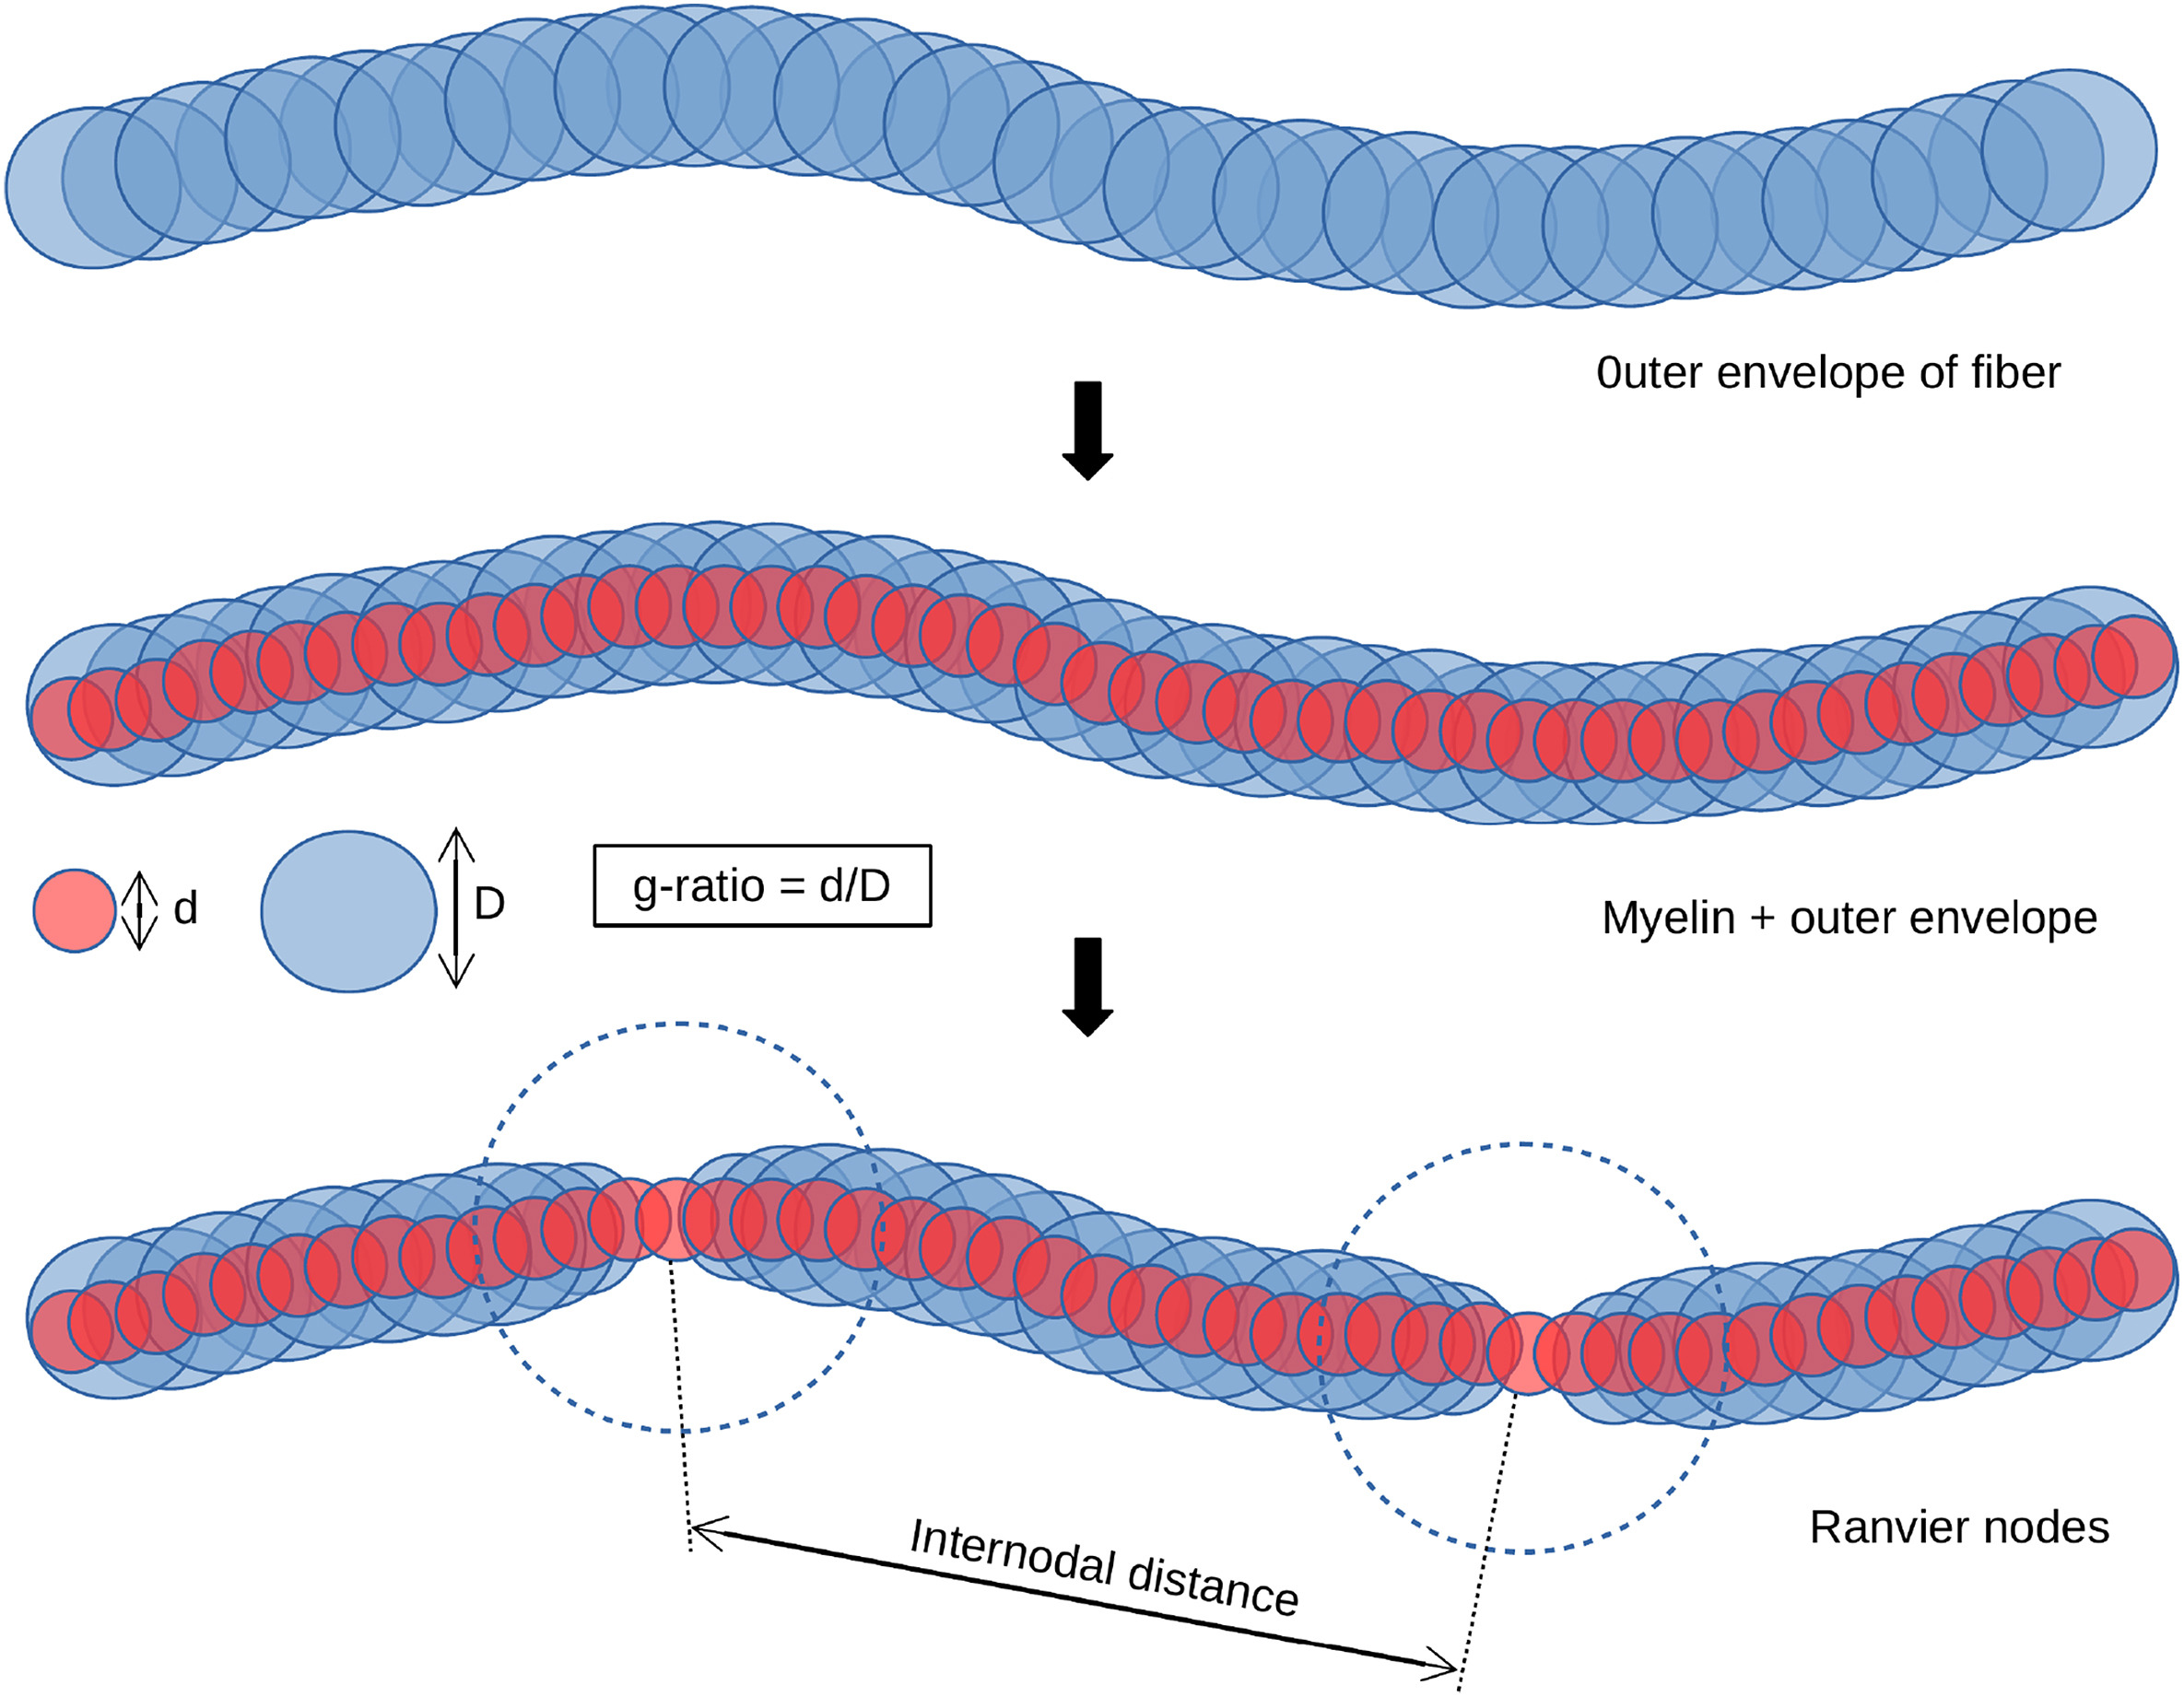
\includegraphics{gfx/model/medusa/4.jpg}
%     % }
% 	\caption{4 \cite{Ginsburger2019}}
% 	\label{fig:model:medusa_4_org}
% \end{figure}
% 
Since all objects are represented as a collection of spheres (see \cref{fig:model:medusa_4})
\begin{align}
    \mathcal{S} = \{ (x_i,y_i,z_i,r_i) : i \in \{0, 1, ..., n_\text{objects}-1\}  \} 
\end{align}
% 
, a collision is present if (VCS !!!)
% 
\begin{align}
\begin{split}
d<r_i+r_j\\
d = \abs{\vv{p}_i - \vv{p}_j}
\end{split}
\end{align}
% 
However since neighboring spheres in one fiber are colliding for a densly populated fiber, they have to be excluded if
\begin{align}
\begin{split}
d(i,j) &\leq  r_i + r_j\\
d(i,j) &= 
\begin{cases}
\sum_{n=i}^{j-1} \abs{\vv{p}_n - \vv{p}_{n+1}},& \text{if } j-i \geq 1\\
0 & \text{otherwise}
\end{cases}
\end{split}
\end{align}
% 
Spheres inside cell bodys are not checked for collision, since their volume aproximate? the volume of the cell.\\
% 
The calculation of collisions is done via the GPU architecture. For this a first implementation was written with the \textit{AxisAligedSortedSearch} \cite{Karras2012}. It sorteds the spheres along one axis, \eg x-axis, and search for each sphere the fist and last possible collision on this axis:
\begin{align}
\begin{split}
\mathcal{C}_i = \{ s \in \mathcal{S} \mid \abs{s_i.x - s_j.x} < r_i+r_j \}
\end{split}
\end{align}
% 
\begin{lstfloat}[!t]
	\lstinputlisting[style=cpp]{code/medusa.cu}
	\caption{Pseudocode of \acs{MEDUSA} collision checking.}
	\label{alg:medusa_collision}
\end{lstfloat}
% 
The above described algorithm is currently used for volumes $\approx \SI{200}{\micro\meter}$. For this volume size the algorithm is for the current use fast enough. However, more advaned algorithm exist wich can be applied here (\eg \textit{BoundindBoxHierarchy} \cite{Karras2012}).
% 
\subsection{Results}
% 
\begin{figure}[!t]
    \centering
    \resizebox{0.95\textwidth}{!}{
    \includegraphics{gfx/model/medusa/8.jpg}}
	\caption{8 \cite{Ginsburger2019}}
	\label{fig:medusa_8}
\end{figure}
% 
\begin{figure}[!t]
    \centering
    \resizebox{0.95\textwidth}{!}{
    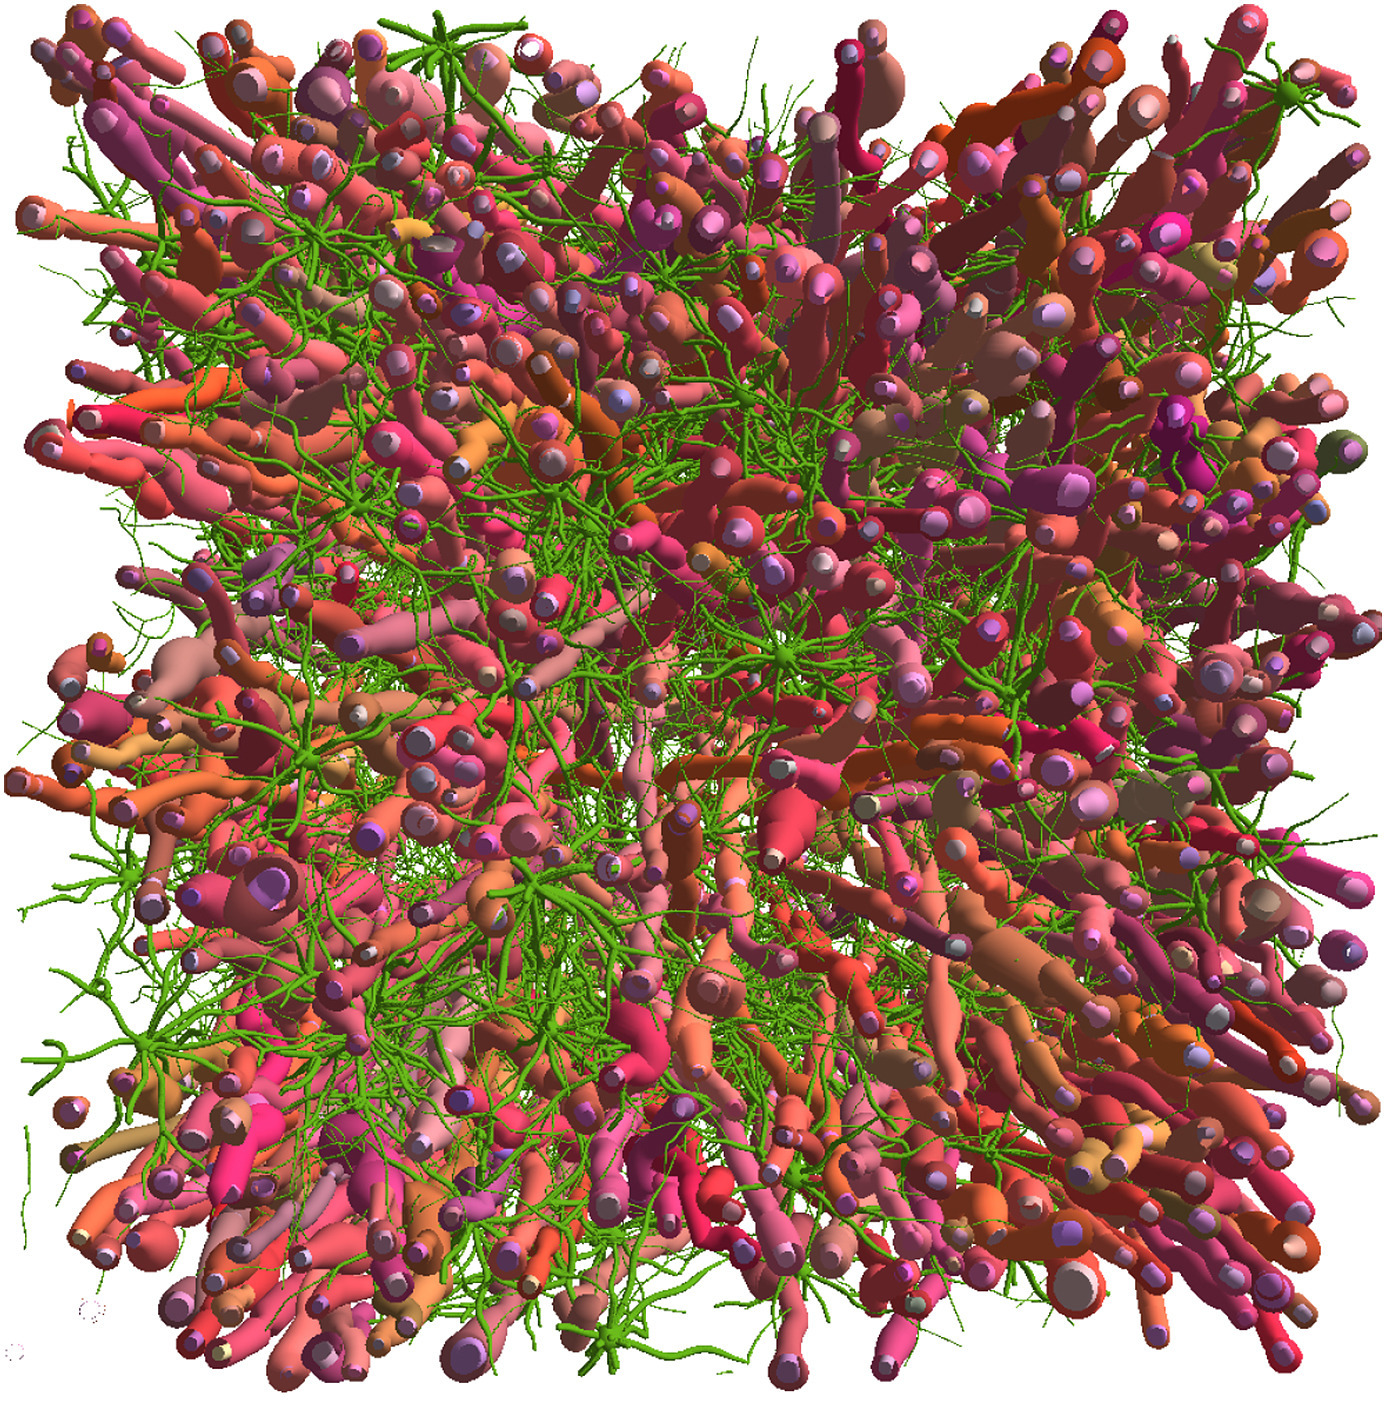
\includegraphics{gfx/model/medusa/11_.jpg}}
	\caption{11 \cite{Ginsburger2019}}
	\label{fig:medusa_11}
\end{figure}
% 
% 
% 
% 
% 
% 
% 
%
% Neurospin works with \ac{dMRI} signals.
% One focus is on the analysis of the fiber architect of the human brain.
% \ac{dMRI} is here quite handy since it is currently the only technique to allow in-vivo measurements to analyse the orientation of white matter tracts. Another importance is the availability of \ac{MRI} machines in almost every hospital in the western civilization.
% Although their resolution is with \SIrange{1.5}{3}{\tesla} limited.
% However, Neurospin is equipped with a mordern \SI{7}{\tesla} \ac{MRI}.
% This makes it possible, including higher measurments times on post mortem brain tissue, a \ac{dMRI} resolution up to \SI{200}{\micro\meter}.
% This makes it possible to allow \ac{3D-PLI} to verify and enhance the analysis of current developed tractography data. 
% %
% Along this works they developed a simulation tool (name) which is computing a Monte-Carlo simulation on the diffusion process in virtual tissues.
% Therefore, for simulations of the \ac{dMRI} signal in the brain, geometric models of nerve fibers as well as nerve cells are required.
% %
% The common goal was, due to a work packes inside the \ac{HBP}, the development of a common general purpose tool to build a geometrical library of nerve fiber configurations.
% Therefore it was decided to work based on the first approaches \cite{Ginsburger2018}.
% %
% \begin{quotation}
% We design a novel white matter numerical phantom generation algorithm which constructs biomimicking geometric configurations with few design parameters, and enables to control the level of disorder of the generated phantoms. The influence of various geometrical parameters present in white matter, such as global angular dispersion, tortuosity, presence of Ranvier nodes, beading, ...
% \end{quotation}
% %
% It is therefore qualified to generate a large database or library of parameter controlled white matter volumes.
% %
% \paragraph{differences:} 
% \begin{itemize}
%     \item All objects are aproximated with spheres.
%     \item Statistical ... of tissue
%     \item diffusion specific parameters
%     \item pathological changes like axon beeding
% \end{itemize}

\cleardoublepage
\setcounter{chapter}{5}
\chapter{\acs{3D-PLI} simulation}
\label{cha:sof:simulation}
%
Simulations of \ac{3D-PLI} have been used to study multiple effects of the microscopic technique involved with brain sections \cite{Dohmen2015,Menzel2015,Menzel2016,Menzel2020,Menzel2021,MenzelMaster,MenzelDissertation}.
The algorithm presented here for designing new collision-free fiber models allowed for the first time to simulate the effect of scattering light in light wave simulations base on finite-difference time domain agorithm without superimposed interference signals.
This enabled the understanding of scattering effects due to fiber bundle and crossing configurations as well as the transmission change for tilted fiber configurations \cite{MenzelDissertation,Menzel2020,Menzel2021}.
\par
% 
In the case of linear optics simulation, the optical system could be successfully simulated and the experimental results could be reproduced \cite{Dohmen2015,Menzel2016}.
The algorithm developed at that time is very computationally intensive and also very memory intensive due to the precomputations of a discretized tissue volume.
The foundations for a more efficient parallel algorithm for supercomputer architecture use were developed in response \cite{Lucksch2016}.
The new tilt design of the LMP3D microscope led to an unnecessary duplication of calculations in the simulations, which could not be easily changed in the algorithm designed at that time.
Therefore, the algorithm was redesigned from scratch.
Additionally, the fiber models presented here had to be incorporated as well.
Finally, the decision was made to switch to the M\"{u}ller-Stokes calculation in order to also take polarization effects of filters into account.
\par
%
The \ac{3D-PLI} simulation is divided into two consecutive parts: the discrete volume generator and the light matter simulation.
The discrete volume generator discretizes the virtual nerve fiber models onto a cartesian grid, which is then used to compute the light-matter interaction in the second step.
A parallelization technique with \ac{MPI} allows the volume to be partitioned among different \acp{CPU} or compute nodes.
Due to the tilting approach, the light vector in such a parallelized volume must be able to leave the current volume of a single \ac{CPU} and traverse to the next volume/process.
The computationally intensive algorithms are written in \cpp{} with an additionally user-friendly designed wrapper function in \python{}.
%
% 
% 
\section{Discrete volume generator}
\label{sec:dv_generator}
%
\begin{figure}[!t]
\centering
\setlength{\tikzwidth}{0.5\textwidth}
\inputtikz{gfx/simpli/disc_volume}
\caption{Discretized tissue volume with a voxel size \voxelsize. The volume is defined by a \ac{AABB}, which itself is defined by two points $\vec{v}_\mathit{min}$ and $\vec{v}_\mathit{max}$.}
\label{fig:discVol}
\end{figure}
%
The \ac{3D-PLI} simulation is to divide the necessary calculations into two consecutive parts. The first part is the calculation of a discretized tissue volume.
It represents a discrete, voxel model of the tissue.
This helps to drastically speed up the light-matter interaction of the next step (see \cref{sec:simulation}), at the cost of a large memory requirement.
\par
%
The discretized tissue volume represents a cuboid divided into smaller cubes of equal size, called voxels, \ie{} 3d pixels (see \cref{fig:discVol}).
Each voxel contains the physical properties absorption, birefringence and optical axis orientation of the tissue at its current position.
The total volume is bounded by a \ac{AABB} or \ac{VOI} defined by a minimum and maximum value $\voi = [(x_{\mathit{min}}, y_{\mathit{min}}, z_{\mathit{min}}), (x_{\mathit{max}}, y_{\mathit{max}}, z_{\mathit{max}})]$.
Additionally, the parameter \Voxelsize{} \voxelsize{} is set to a floating point number and defines the edge length of the equilateral voxels.
If the division of any of the \voi{} axis by \voxelsize{} is not an integer, the corresponding axis of the \voi{} is incremented to the nearest possible integer value to avoid edge effects.
%
%
%
\subsection{Nerve fiber layers}
%
As described in \cref{sec:fiberArchitecture}, nerve fibers are axons that can be wrapped by multiple turns of myelin (see \cref{fig:myelinLayer}).
Especially for light wave simulations, the myelin windings are an important feature \cite{MenzelDissertation}.
\par
%
The windings are represented as individual layers (see \cref{fig:fiberLayer}).
This greatly simplifies the creation process.
A layer is defined by a factor between $\SI{0}{}$ and $\SI{1}{}$ that scales with the radius of the nerve fiber.
For example, $\SI{0.75}{}$ means that from $0 \leq r < 0.75$ of the radii is interpreted as the first layer (see \cref{fig:fiberLayer}).
\par
%
Each layer requires a number of physical properties in addition to its radius:
%
\begin{itemize}[nosep]
    \item birefringence value: $\dn$
    \item absorption coefficient: $\mu$
    \item optical axsis model: $p=\mathit{parallel}$, $r=\mathit{radial}$, $b=\mathit{background}$
\end{itemize}
%
These properties are specified as a list of tuples within the algorithm (see \cref{alg:fiberbundleprops}).
%
%
At the end, the discretize volume generator returns the arrays \tissue{}, \opticalaxis{} and \propertylist{} for use in the light matter simulation.
Since the arrays are quite large, the transfer is performed as a ownership movemend of a \name{numpy-array} without having to copy the data.
% 
\begin{lstfloat}[!ht]
\lstset{style=python}
\begin{lstlisting}[]
fbs_properties = [[(r, dn, mu, 'p'), (second layer), ...],
                  [(first layer of second bundle), ...],
                  [...]]
\end{lstlisting}
\caption{Definition of the properties of fiber bundles.}
\label{alg:fiberbundleprops}
\end{lstfloat}
% 
% 
% 
\subsection{Discretization of a nerve fiber model}
%
\begin{figure}[!t]
\centering
\setlength{\tikzwidth}{0.3\textwidth}
\subcaptionbox{\label{fig:myelinLayer}Schematic representation of a nerve fiber with axon and myelin sheath}
[\tikzwidth]{\includegraphics[height=\tikzwidth]{dev/brain/myelin_layers.pdf}\vspace{0mm}}\hfill
\subcaptionbox{\label{fig:fiberLayer}Cross section through a nerve fiber with layered structure defined by $n$ radii}
[\tikzwidth]{\inputtikz{gfx/simpli/fiber_layer}\vspace{-5mm}}\hfill
\subcaptionbox{\label{fig:vectormodel}Cross section of a discretized nerve fiber with resulting optical axis vectors}
[\tikzwidth]{\inputtikz{gfx/simpli/vector_model}\vspace{-5mm}}
\caption{Discretization of nerve fibers with layered structure.}
\label{fig:fiber_discretization}
\end{figure}
%
To discretize nerve fiber models individual nerve fiber segment are discretized after each other, since a fiber is a chain of consecutive segments.
Each voxel inside a fiber segment has to be labled as a tissue with the physical properties at the voxel center position $\vec{q}$ (see \cref{fig:fiber_discretization}).
The discretized mesh represents an array, where an element at position $[i,j,k]$ occupies the space from $(i,j,k)$ to $(i+1,j+1,k+1)$ in the unit of $\SI{1}{\voxelsize}$.
\par
%
To identify all voxels inside a volume all voxels inside the fiber segments are checked if they are inside the fiber segment.
Therefore a loop over all voxels is performed.
\par
%
To calculate if a voxels is inside the nerve fiber segment,
a computation analogously to the collision between two nerve fiber segments is calculated (see \cref{alg:pseudocodeCollisionDetection}).
The difference is, that only one point on a the fiber segment line has to be calculated.
The second point is the voxels center $\vec{q}$.
From this calculation, not only the nearest points $\vec{p}_a$ and $\vec{p}_b$ are returned, but also the distance vector $\vec{d}$.
The distance of the vector is used to check whether the voxel is inside the fiber segment, and if so, in which layer of the fiber segment it is located.
if the optical axis orientation follows a macroscopic model, the points $\vec{p}_a, \vec{p}_b$ are used to calculate the orientation.
\par
%
In case of a voxel occupied by a fiber segment, two values are stored.
The first one is an index within an array \name{tissue} which will be used later to retrieve the properties from a list with the same index order.
The second information is the orientation of the optical axis within the current layer, stored in the array \name{optical\_axis}.
The orientation is either parallel to the fiber segment in the case of the macroscopic model, or radial in the case of the microscopic model.
A layer can also be marked as \say{background}, allowing the user to specify an area without any birefringence.
\par
%
The next step is to loop aver all fiber segments and fill the volume.
However, another problem must be solved first.
Since two consecutive fiber segments occupy the same space because they have a common point, they also fill some voxels of the tissue volume simultaneously.
This is a problem because the processed second fiber segment overwrites the values of the first.
This is solved by using an additional array that stores the smallest distance calculated when filling the voxels space.
The values are only overwritten when a new distance is calculated that is smaller than the one already stored.
This solves also the problem that in a radial optical axis model, the optical axis is star-shaped at the end points of each fiber segment inside the fiber.
The first and last point of a fiber, however, are not affected by this.
\par
%
The algorithm for the discretization loop is shown in \cref{alg:fillVolume}.
%
\begin{lstfloat}[!tb]
\lstset{style=python}
\begin{lstlisting}[]
for fiber_segment in fiber_bundle:
    for i,j,k in fiber_segment.aabb().voxels():
        min_dist, min_point = calculate_min_distance((i,j,k), cc)
        if min_dist < cc.radius:
            if min_dist < current_distance[i,j,k]:
                optical_axis[i,j,k,:] = get_axis_orientation(
                                            (i,j,k), min_dist,
                                            min_point)
                tissue[i,j,k] = get_layer_id(min_dist)
                current_distance[i,j,k] = min_dist
\end{lstlisting}
\caption{Pseudocode for filling the discretized volume.}
\label{alg:fillVolume}
\end{lstfloat}
%
\paragraph{Additional Information}
Since the light matter simulation algorithm recieves an \name{tissue}, \name{optical\_axis} and \name{propertie} array, the user can also change the values in between both algorithms.
In the upper algorithm, the optical axis vectors length is $\SI{1}{}$.
The length of the vector is in the light matter simulation part interpreted as the birefringence strength factor.
Therefore the user can \eg{} add additionall variability of the strength of the birefringence.
%
%
%
\subsection{\Voxelsize}
%
\begin{figure}[!t]
\centering
% \tikzset{external/export=false}
\setlength{\tikzwidth}{.24\textwidth}
\definecolor{c1}{rgb}{0.25,0.4,0.1}
\definecolor{c2}{rgb}{1.0,0.73,0}
\definecolor{c3}{rgb}{0.98,0.4,0.25}
\definecolor{c4}{rgb}{0.22,0.36,0.59}
%
% \definecolor{c1}{HTML}{440154FF}
% \definecolor{c2}{HTML}{38598CFF}
% \definecolor{c3}{HTML}{1E9B8AFF}
% \definecolor{c4}{HTML}{FDE725FF}
%
\def\xc{0.7}
\def\yc{0.2}
\def\rin{1.5}
\def\rout{3}
%
% 
\newcommand{\fiber}[3]{
	\def\dd{#1}
	\pgfmathsetmacro{\xmin}{int(floor(\xc-\rout))}
	\pgfmathsetmacro{\xmax}{int(ceil(\xc+\rout))}
	\pgfmathsetmacro{\xd}{\xmin+\dd}
	\pgfmathsetmacro{\ymin}{int(floor(\yc-\rout))}
	\pgfmathsetmacro{\ymax}{int(ceil(\yc+\rout))}
	\pgfmathsetmacro{\yd}{\ymin+\dd}
	%
	\pgfmathsetmacro{\rmin}{\rin*\rin*100}
	\pgfmathsetmacro{\rmax}{\rout*\rout*100}
	\foreach \x in {\xmin,\xd,...,\xmax} {
		\foreach \y in {\ymin,\yd,...,\ymax} {
			\pgfmathsetmacro{\d}{int(((\x-\xc+\dd/2)*(\x-\xc+\dd/2)+(\y-\yc+\dd/2)*(\y-\yc+\dd/2))*100)}
			\ifnum\d>\rmin
			\ifnum\d<\rmax
			\path [#3] (\x,\y) rectangle ($ (\x, \y) + (\dd, \dd) $);
			\draw[#2] ($ (\x, \y) + (0, 0) $) -- ($ (\x, \y) + (\dd, 0) $);
			\draw[#2] ($ (\x, \y) + (\dd, 0) $) -- ($ (\x, \y) + (\dd, \dd) $);
			\draw[#2] ($ (\x, \y) + (\dd, \dd) $) -- ($ (\x, \y) + (0, \dd) $);
			\draw[#2] ($ (\x, \y) + (0, \dd) $) -- ($ (\x, \y) + (0, 0) $);
			\fi\fi
		}
	}
%	\foreach \x in {\xmin,\xd,...,\xmax} {
%		\draw[#2] (\x,\ymin) -- (\x,\ymax);
%	}
%	\foreach \y in {\ymin,\yd,...,\ymax} {
%		\draw[#2] (\xmin,\y) -- (\xmax,\y);
%	}
}
%
\subcaptionbox{}[\tikzwidth]{
\resizebox{\tikzwidth}{!}{
\begin{tikzpicture}[]
\path[] (-3.75, -3.5) rectangle (3.75, 3.25);
\begin{scope}[shift={(-\xc,-\yc)}]
\fiber{2}{line width = 0.2mm}{pattern color=c1,pattern=horizontal lines}
\draw[line width = 0.4mm] (\xc,\yc) circle (\rin);
\draw[line width = 0.4mm] (\xc,\yc) circle (\rout);
\end{scope}
\end{tikzpicture}
}}
\hfill
%
\subcaptionbox{}[\tikzwidth]{
\resizebox{\tikzwidth}{!}{
\begin{tikzpicture}[]
\path[] (-3.75, -3.5) rectangle (3.75, 3.25);
\begin{scope}[shift={(-\xc,-\yc)}]
\fiber{1}{line width = 0.1mm}{pattern color=c2,pattern=vertical lines}
\draw[line width = 0.4mm] (\xc,\yc) circle (\rin);
\draw[line width = 0.4mm] (\xc,\yc) circle (\rout);
\end{scope}
\end{tikzpicture}
}}
\hfill
%
\subcaptionbox{}[\tikzwidth]{
\resizebox{\tikzwidth}{!}{
\begin{tikzpicture}[]
\path[] (-3.75, -3.5) rectangle (3.75, 3.25);
\begin{scope}[shift={(-\xc,-\yc)}]
\fiber{0.5}{line width = 0.05mm}{pattern color=c3,pattern=north east lines}
\draw[line width = 0.4mm] (\xc,\yc) circle (\rin);
\draw[line width = 0.4mm] (\xc,\yc) circle (\rout);
\end{scope}
\end{tikzpicture}
}}
\hfill
%
\subcaptionbox{}[\tikzwidth]{
\resizebox{\tikzwidth}{!}{
\begin{tikzpicture}[]
\path[] (-3.75, -3.5) rectangle (3.75, 3.25);
\begin{scope}[shift={(-\xc,-\yc)}]
\fiber{0.25}{line width = 0.025mm}{pattern color=c4,pattern=crosshatch dots}
\draw[line width = 0.4mm] (\xc,\yc) circle (\rin);
\draw[line width = 0.4mm] (\xc,\yc) circle (\rout);
\end{scope}
% \fiber{2}{}{fill, c1, opacity=0.25}
% \fiber{1}{very thin}{fill, c2, opacity=0.25}
% \fiber{0.5}{ultra thin}{fill, c3, opacity=0.25}
% \fiber{0.25}{ultra thin}{fill, c4, opacity=0.25}
%
\end{tikzpicture}
}}
\caption{Discretization error. Cross-section through a single fiber with a myelin layer in the discretized tissue volume. The colored pattern shows the resulting voxels corresponding to the fiber. The smaller the \Voxelsize, the smaller the discretization error.}
\label{fig:vectorfield_disc_error}
\end{figure}
%
The parameter \Voxelsize{} is a very important property of the light matter simulation.
It determines how accurate the volume is represented (see \cref{fig:vectorfield_disc_error}).
Additionally the in the light matter simulation one light ray is casted from each voxel of the bottom plane (see \cref{sec:pathOfLight}). 
Therefore it is also responisble for the sampling of the resulting intensities.
%
%
% 
\subsection{Optimizations}\label{sec:dvOpti}
%
All arrays are implemented as contiguous c-arrays, accessible externally as \name{numpy-arrays} without the need to copy the data.
Since these arrays grow with $\mathcal{O}(\frac{1}{\voxelsize}^3)$, the ownership of the data is movable in both the \cpp{} libraries and \python{} code.
The memory order of the arrays is in the $x\text{-}y\text{-}z$ direction, so the largest memory shift is in $x$ and the smallest in $z$.
This was chosen so that later in the light matter simulation part, where the light moves mainly in the $z$-direction, the memory is aligned with the traversed information and thus the \acp{CPU} cache prefetcher can be used effectively.
\par
%
Two methods are used to parallelize the algorithm on the \ac{CPU}.
The first uses \ac{OpenMP} to parallelize the filling of the \ac{AABB} volume of each object.
The second uses \ac{MPI} to allow distribution across multiple \ac{CPU} cores without sharing memory (detailed description in \cref{sec:mpiSim}).
\par
%
Parallelizing the filling prozess of the voxels of the discretized volume leads to a race condition when multiple threads want to write or read to the same memory address, \ie{} the same coordinate in the volume.
A solution with a lock would be very slow and since many of the voxels do not need to be overwritten, most of the locks would be unnecessary.
To share the work, thread $n$ processes only the memory for the first index $i$ (or volume dimension $x$) if:
%
\begin{align}
\begin{split}
    i \bmod N_{\mathit{Threads}} == \mathit{thread}_{\mathit{id}}
\end{split}
\end{align}
%
\begin{figure}[!t]
\centering
\setlength{\tikzwidth}{0.5\textwidth}
\inputtikz{gfx/simpli/disc_volume_thread}
\caption{Discretization volume parallelization with \ac{OpenMP}. Each thread processes every $n$-th $yz$-section. This ensures both thread safety and a more balanced workload, even under inhomogeneous conditions.}
\label{fig:discVolThread}
\end{figure}
% 
This means that each thread loops over every $N_{\mathit{num\_threads}}$ slice of the volume (see \cref{fig:discVolThread}).
This is done instead of dividing the volume to n sub volumes to distribute the work in case that the volume is not filled homogeniously with fibers.
This procedure leads to a thread-safe writable operation.
One disatvantage of this algorithm is, that all threads have to check if the \ac{AABB} of all fiber segments is inside the current \ac{VOI}.
% 
% 
%
\section{Light matter Simulation}
\label{sec:simulation}
%
The light matter simulation algorithm performs the Mueller-Stokes calculation (see \cref{sec:Mueller-Stokes}) on the previously calculated discrete volume (see \cref{sec:dv_generator}) for the light rays along their paths.
Since no scattering or refraction effects are considered in this simulation, each light path follows a straight line.
Initially, the light vector is multiplied by the first polarizer of the optical system (see \cref{sec:expSetup}).
The path inside the tissue is discretized into steps.
The interaction between the light ray and the tissue is calculated after each step according to $ \vec{S}' = \prod_i \left(\mat{R}_i \mat{M}_i \mat{R}_i\right) \cdot \vec{S}$ (see \cref{sec:mueller_stokes, sec:simLightTissue}).
% After a light beam reaches the end of the tissue, the last optical elements of the setup are applied to the lights vector.
% Finally, the light intensity is stored in the \acs{CCD} image array, which at this point of the algorithm has the same size as the 2d $xy$ grid of the discretized tissue.
% In a later step, the intensities will be blurred and resampled to the acually \ac{CCD} pixels size and noise will we added according to the users specifications.
% 
%
%
\subsection{Light ray path}
\label{sec:pathOfLight}
%
\begin{figure}[!t]
\setlength{\tikzheight}{0.42\textwidth}
\subcaptionbox{camera view}
[.475\textwidth]{\inputtikz{gfx/simpli/tilting_3d_a}}\hfill
\subcaptionbox{perspective view}
[.475\textwidth]{\inputtikz{gfx/simpli/tilting_3d_b}}
\tikzset{external/export=false}
\caption[3d tilting]{3d tilting: around $xy$-axis, \raisebox{.25em}{\tikz \draw[red,thick](0,0)--(0.25,0);} top, \raisebox{.25em}{\tikz \draw[green,thick](0,0)--(0.25,0);} middle, \raisebox{.25em}{\tikz \draw[blue,thick](0,0)--(0.25,0);} bottom, \raisebox{.25em}{\tikz \draw[dash pattern=on 1.25pt off 1.25pt,thick](0,0)--(0.25,0);} original, \raisebox{.25em}{\tikz \draw[gray](0,0)--(0.25,0);} axis of rotation.}
\label{fig:tilting_camera_view}
\end{figure}
%
The light matter simulation allows for a tilting light beam.
For this purpose, the \ac{LAP} uses a tilting stage to which the tissue sections are attached (see \cref{fig:tilting_camera_view}).
The \ac{LMP3D}, on the other hand, has an tilted light beam.
This is achieved by a conical light path, from which an aperture is then used to sample the desired light direction \cite{Wiese:887678}.
Both methods can be mathematically represented by the same procedure.
\par
%
An additional effect changing the light path is the refraction at the tissue-air boundary, which is described by Snell's law for isotropic media (see \cref{eq:Snellius}).
Since this only adds a parallel shift, simulation is only necessary when the effects of the resampling process and image registration is to be investigated.
\par
%
\begin{figure}[!t]
\setlength{\tikzwidth}{0.45\textwidth}
\subcaptionbox{normal}[.475\textwidth]{
\def\tilt{0}
\def\nindex{2.25}
\inputtikz{gfx/simpli/tilting_a}}\hfill
\subcaptionbox{tilted}[.475\textwidth]{
\inputtikz{gfx/simpli/tilting_b}}
\caption[Light path]{Light ray path for a normal (a) and a tilted (b) case. In the tilted case, the light beam $\vec{l}_1$ is tilted within the tissue and thus experiences an optical shift $\Delta$.}
\label{fig:tilted_side_view}
\end{figure}
%
The initial position of the light beam is calculated by traversing the light path backwards (see \cref{fig:tilted_side_view}).
This has the advantage, that the each index inside the \ac{CCD} receives always exactly one light beam.

From the \ac{CCD} array, the light path can be shifted back to the top plane of the tissue $\mathfrak{S}_{top}$.
Subsequently, the light beam $\vec{l}_1$ is traced back through the tissue to the bottom plane $\mathfrak{S}_{bottom}$.
The point on the lower tissue plane corresponds to the initial position of the light beam.
This light path change results in a shift $\delta$ along the same direction of the tilting.
In the light matter simulation only light rays are considered, which will go at least partially through the volume.
All remaining \ac{CCD} elements are left with a \textit{NaN} value.
\par
%
The tilting of the tissue leads to a distortion of the image (see \cref{fig:tilting_camera_view}).
This distortion can be described by an affine transformation (see \cref{fig::affine_transformation}):
%
\begin{figure}[!t]
\centering
\pgfmathsetmacro{\size}{10}
% 
\subcaptionbox{}[.225\textwidth]{
\resizebox{.225\textwidth}{!}{
\begin{tikzpicture}[]
\pgfmathsetmacro{\dx}{2.25}
\pgfmathsetmacro{\dy}{1.5}
\draw[help lines] (0,0) grid (\size,\size);
\foreach \i in {0,...,\size}{
	\draw [very thick] (\i+\dx, 0+\dy) -- (\i+\dx, \size+\dy);
	\draw [very thick] (0+\dx, \i+\dy) -- (\size+\dx, \i+\dy);
}
\end{tikzpicture}
}}
% 
\subcaptionbox{}[.225\textwidth]{
\resizebox{.225\textwidth}{!}{
\begin{tikzpicture}[]
\pgfmathsetmacro{\sx}{1.5}
\pgfmathsetmacro{\sy}{0.75}
\draw[help lines] (0,0) grid (\size,\size);
\foreach \i in {0,...,\size}{
	\draw [very thick] ({\i*\sx}, 0) -- ({\i*\sx}, {\size*\sy});
	\draw [very thick] (0, {\i*\sy}) -- ({\size*\sx}, {\i*\sy});
}
\end{tikzpicture}
}}
%
\subcaptionbox{}[.225\textwidth]{
\resizebox{.225\textwidth}{!}{
\begin{tikzpicture}[]
\draw[help lines] (0,0) grid (\size,\size);
\begin{scope}[rotate around={30:(0.5*\size,0.5*\size)}]
\foreach \i in {0,...,\size}{
	\draw [very thick] (\i, 0) -- (\i, \size);
	\draw [very thick] (0, \i) -- (\size, \i);
}
\end{scope}
\end{tikzpicture}
}}
% 
\subcaptionbox{}[.225\textwidth]{
\resizebox{.225\textwidth}{!}{
\begin{tikzpicture}[]
\pgfmathsetmacro{\cx}{0.5}
\pgfmathsetmacro{\cy}{0}
\draw[help lines] (0,0) grid (\size,\size);
\foreach \i in {0,...,\size}{
	\draw [very thick] (\i+0*\cx, 0+\i*\cy) -- (\i+\size*\cx, \size+\i*\cy);
	\draw [very thick] (0+\i*\cx, \i+0*\cy) -- (\size+\i*\cx, \i+\size*\cy);
}
\end{tikzpicture}
}}
\caption{affine transformation}
\label{fig::affine_transformation}
\end{figure}
%
\begin{align}
f(\vec{x}) = \mat{A} \cdot \vec{x} + \vec{t}
\end{align}
where $\vec{x}$ is the coordinate input, $\mat{A}$ and $\vec{t}$ are the transformation values, and $f(\vec{x}$ is the transformed coordinate.
\par
%
The light matter simulation with the light paths sampling as described above takes this distorted view into acount and removes it.
The simulation is also capable of sampling the light rays in such a way, that the distortion occurs.
In that case the resulting images have to be registered onto each other \eg{} by an affine transformation wich is also available.
% 
% 
% 
\subsection{Tissue voxel interpolation}
%
If the \Stepsize{} of the light ray is not equal to the \Voxelsize{} or if the light path is tilted, the light rays position after a step does not longer matches the center of the voxel.
This means that the physical properties stored in the arrays have to be interpolated.
%
\begin{figure}[!t]
\centering
\setlength{\tikzwidth}{0.475\textwidth}
% \tikzset{external/force remake=true}
\subcaptionbox{\label{fig:triInterp}Trilinear interpolation}
[\tikzwidth]{
\hfill\inputtikz{gfx/simpli/trilinear_interpolation}\hfill}\hfill
\subcaptionbox{\label{fig:sphInterp}Spherical interpolation}
[\tikzwidth]{
\inputtikz{gfx/simpli/vector_interpolation}}
\caption{Interpolation techniques: Trilinear interpolation can be represented as an axial step interpolation. The difference between linear and spherical interpolation is that linear interpolation has a constant distance $s$ between each point, while spherical interpolation has a constant angle $\varphi$ between two steps.}
\label{fig:vectorfield_disc}
\end{figure}
%
Currently three interpolation methods are implemented: \name{nearest neighbor}, \name{linear interpolation} and \name{spherical interpolation}.
The voxels considered for interpolation are the nearest eight neighboring voxels, i.e. array indices $(\floor{x\pm0.5},\floor{y\pm0.5},\floor{y\pm0.5})$.
The \name{nearest neighbor} and \name{linear interpolation} are still present from the development phase.
However, they should not be used because they are error-prone.
Since the data are orientations, the default value for the interpolation method \name{spherical interpolation} should be used.
%
%
%
\subsection{Simulation of light matter interaction}\label{sec:simLightTissue}
%
After the initial light positions are calculated each light beam is traversed within the tissue.
To calculate the light-tissue interaction, the change of the Stokes vector is calculated after each light beam step.
The step size is a user defined value with a default value of the \Voxelsize{} $\voxelsize$.
Once the light hits the boundary of the volume, the light beam is multiplied by the matrix of the remaining optical elements of the microscop and the intensity is stored in the \ac{CCD}-array.
The pseudocode is shown in \cref{alg:simulationLoop}.
%
\begin{lstfloat}[!tb]
\lstset{style=python}
\begin{lstlisting}[]
light_beams = calculate_light_starting_positions()

for light in light_beams:
    light = optical_elemts_start * light
    while light.pos in volume:
        properties = get_properties(light.pos)
        light.intensity *= exp(-step_size * properties.absorbtion)
        light = matrix(properties) * light
        light.pos += step_size
   
    light = optical_elemts_end * light
    ccd_array[light.ccd_pos] = light.intensity
\end{lstlisting}
\caption{Loop over the light vectors for the light-tissue interaction. Their intensity value is stored inside the \ac{CCD} array.}
\label{alg:simulationLoop}
\end{lstfloat}
%
To resample the array to the final size of the \ac{CCD} sensor and apply noise model python funcions exits outside of the parralized simulation software.
% 
% 
%
\subsection{Optimizations}
%
Several optimizations exists in this pipeline.
First, the order of the tissues stored in memory is along the z-axis (as described in \cref{sec:dvOpti}) so that the light ray \textit{traverses} along the aligned memory.
Second, the for-loop for the light beams (see \cref{alg:simulationLoop}) is paralellized with \ac{OpenMP}.
These threads are completely separated and there are no race conditions.
In addition, all vector and matrix calculations are optimized for their small sizes by the compiler with the help of tools like \name{Compiler Explorer}\footnote{\url{https://godbolt.org/}} and \name{C++ Insight}\footnote{\url{https://cppinsights.io/}}.
%
%
\section{Optical system and signal analysis}
\label{sec:ccdOptic}
%
The image sensor, as described in \cref{sec:expSetup}, is a \ac{CCD}-sensor.
The the resampling and noise modeling, are implemented according to \cref{sec:opticalResolution}.
These calculations are performed on the \python{} side of the algorithm (\code{fastpli.simulation.Simpli}) and can be executed with the \code{multiprocessing} library of \python{} to use multiple \ac{CPU} cores.
Therefore when using \ac{MPI} (see \cref{sec:mpiSim}) the intensity image has to be reduced to a single process.
Since this image is only two dimensional, there is no need to speed up the process with \ac{MPI} further.
\par
%
To analyse the signal, the same algorithms are implemented as in the \ac{3D-PLI} routine pipeline (see \cref{sec::intSignal,sec::InclAnalysis}).
This include the modalities analysis transmittance, direction and retardatation as well as the tilting analysis performend by \ac{ROFL}.
The tilting analysis takes quite a lot time.
Therefore it can also be executed with the \code{multiprocessing} library of \python{}.
%
%
%
\section{MPI parallelization}\label{sec:mpiSim}
%
Both algorithms, the discrete volume generator and the light matter simulation, can additionally use a parallelization technique.
For large volumes that are larger than the local memory size, the computation must be split among multiple physical \acp{CPU}s and \name{computation nodes}.
For this purpose, \acreset{MPI} \ac{MPI} is used.
A method is implemented to automatically partition the volume along the $x$-axis and the $y$-axis into blocks with minimal surface area along both axis (see \cref{fig:com_halo}).
\par
% 
Each \ac{CPU} can performed the discrete volume generation without the knowlege of each other.
The exception is the light matter simulation for tilted light beams.
Here, when a light ray leaves the local volume, it must be transmitted to the adjacent volume.
\ac{MPI} provides several methods to send information to another \name{rank}.
Since the subvolumes are splitted along a cartesion grid, the cartesion implementations of \ac{MPI} are used (\eg{} \code{MPI\tu Cart\tu create}).
%
\begin{figure}[!t]
    \centering
    \setlength{\tikzwidth}{0.85\textwidth}
    \inputtikz{gfx/simpli/com_halo}
    \caption{ This example uses six \ac{MPI} ranks to split the entire volume into six subvolumes. To calculate the value at a given point a eight-neighborhood is necessary. Therefore a \name{halo} area (coloured voxels) with the same information shared by neighboring \ac{MPI} process is necesarry.}
    \label{fig:com_halo}
\end{figure}
%
A problem is the calculation at the edge of the volume, because the light beam needs the information of the surrounding eight voxels for the interpolation.
If this voxel information were to be transmitted to the neighboring \name{rank} as well, this would mean a large amount of communication, which is much slower compared to the local \ac{CPU} or \ac{RAM} instructions.
The solution is a so-called \name{halo}.
This is a commonly used concept where the boundaries (in this case a volume) are increased by a certain size (in this case $\SI{1}{\voxel}$) so that the same information about the shared regions is available everywhere (see \cref{fig:com_halo}).
\par
%
With this concept, only the light beam needs to be communicated to the neighbors when leaving the local volume (see \cref{fig:com_halo}).
This is also the reason why the surface area is minimized, so the number of communications is also minimized.
\par
% 
To further speed up the communication process, all outgoing light beams are first stored locally in a communication buffer, and only after all local light beams have been processed is the buffer passed on to the neighbors.
This ensures minimal communication overhead.
The main loop of the light beam algorithm is then restarted on all \ac{MPI} \name{ranks} for the communicated light beams.
This is repeated until no more communication is required.
\par
%
Each \ac{MPI} process can additionally use \ac{OpenMP} to allow multiple cores to benefit from shared memory.
\cleardoublepage
\setcounter{chapter}{6}
\chapter{\acs{fastPLI}}
\label{chap:Software}
% 
% 
% 
\section{Introduction}\label{sec:fastpliIntro}
%
The previous chapters described the algorithms for creating dense \ac{WM} fiber models (see \cref{chap:sof:modelling}) and for simulating such models in \ac{3D-PLI} (see \cref{cha:sof:simulation}).
Both algorithms are designed to operate autonomously without knowledge of the other.
This can simplify the use of the algorithms for other domains.
For example, the fiber models can be used in \ac{dMRI} as well (\cite{Ginsburger2019,ginsburgerDis2019}).

These algorithms are designed to be fast.
This usually means code design with very few abstractions.
Therefore, an \ac{API} is needed on top of the algorithms, which provide a user interface which is easy to use.
Among other things, this means a high level of abstraction.
In addition, the algorithms should be easily installable to provide easy access.
\par
%
In summary, this means that a software package must be developed that contains the algorithms and helper functions.
For the above reasons, the \python{} programming language was chosen.
It has become increasingly popular over the last decade, especially in data science.
The core algorithms remain in \cpp{} as described in their chapters to ensure efficiency, speed, and parallelization.
%
% 
% 
\section{fastPLI Toolbox}
%
\begin{figure}[!ht]
\centering
\inputtikz{gfx/fastpli/fastpli_pipeline}
\caption{\acs{fastPLI} package structure.}
\label{fig:fastpli}
\end{figure}
%
The here designed \python{} package is called \acreset{fastPLI} \ac{fastPLI}.
Its source code is publicly available and reviewed in the \ac{JOSS} \cite{fastpli,Matuschke2021}.
The software package includes functionalities for the analysis and visualization of the nerve fiber models as well as for the analysis of the simulation analogous to the current routine experimental measurements, \eg{} tilt analysis (see \cref{fig:fastpli}).
%
%
%
\subsection{Documentation}
%
\begin{figure}[!t]
    \centering
    \resizebox{\textwidth}{!}{\fbox{
    \begin{tabular}{c|c}
    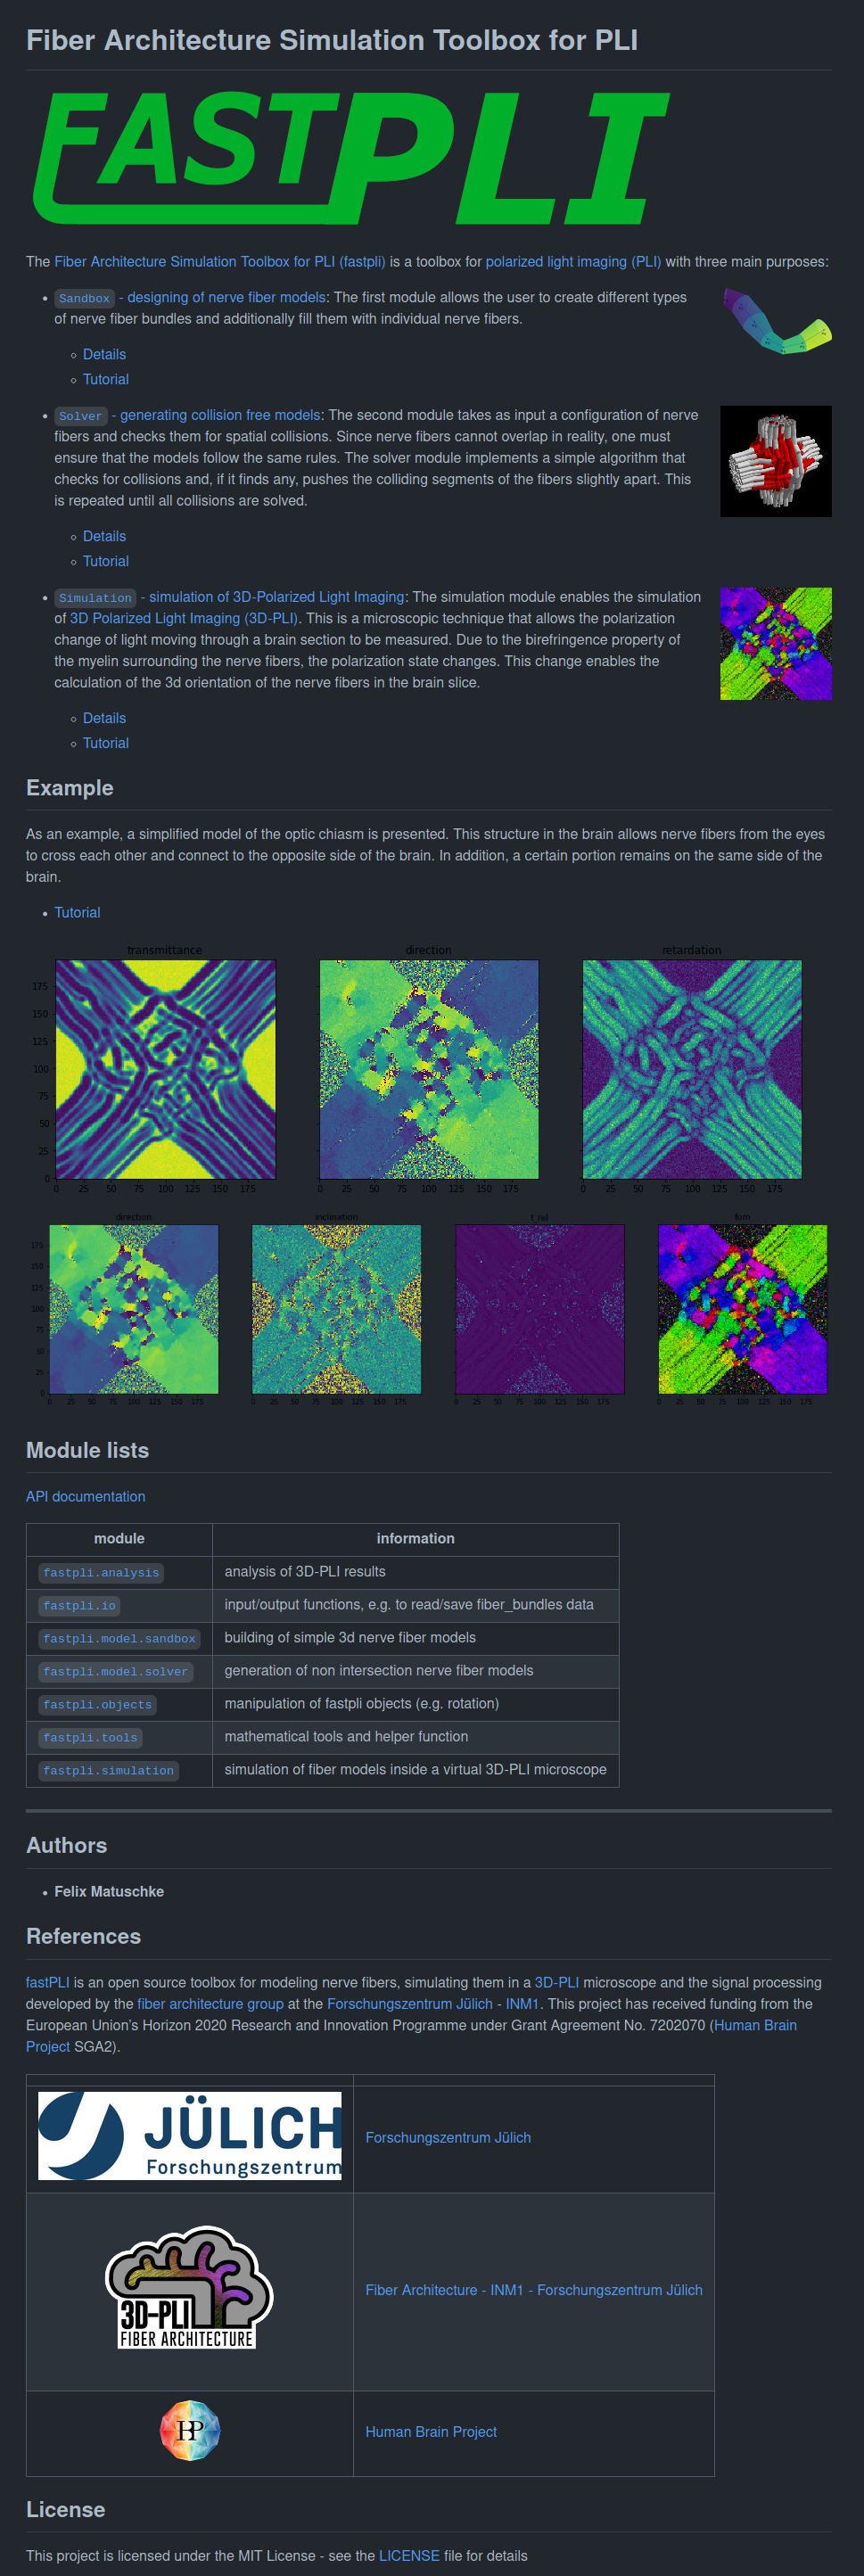
\includegraphics[valign=T,trim=0 1300 0 0, clip]{gfx/fastpli/fastpli_wiki.png} &
 	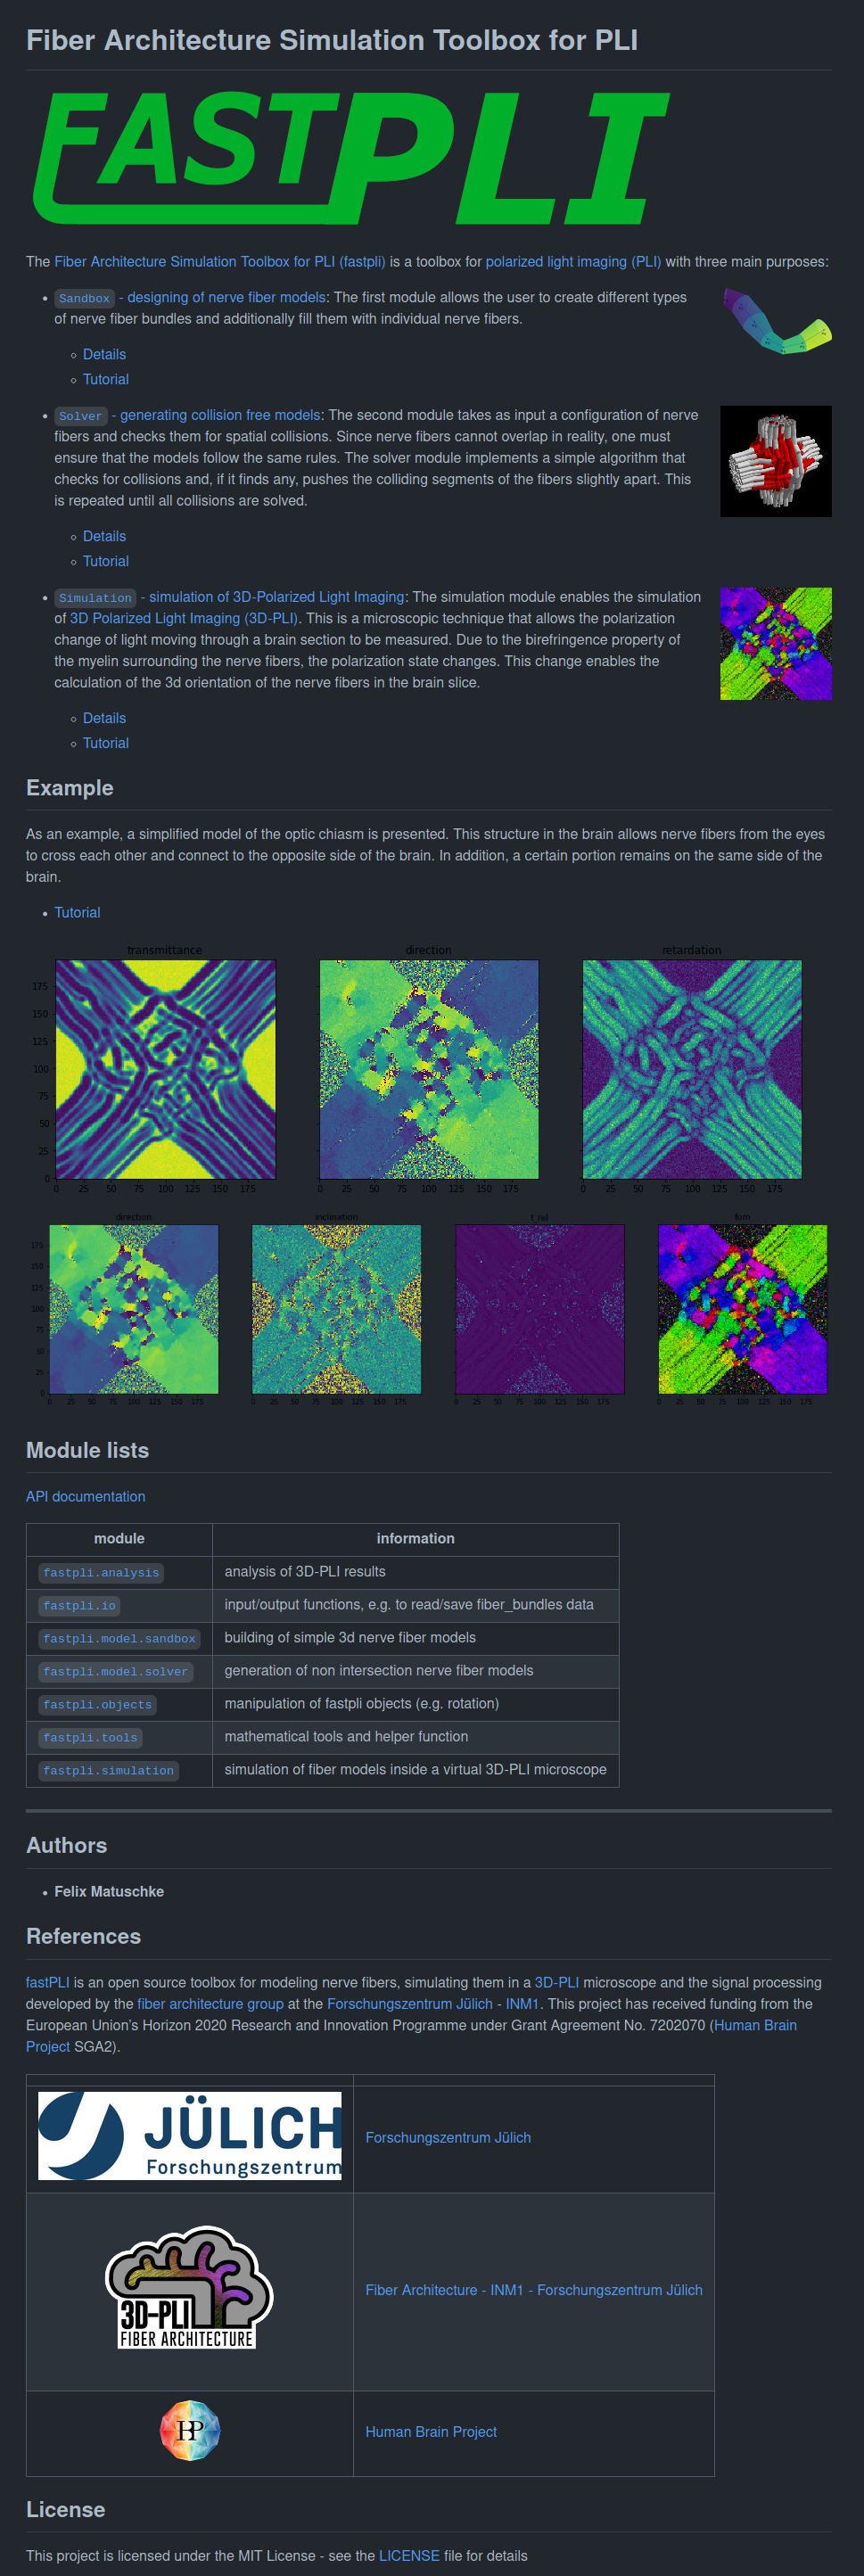
\includegraphics[valign=T,trim=0 0 0 1580, clip]{gfx/fastpli/fastpli_wiki.png} \\
    \end{tabular}
    }}
	\caption{Documentation wiki page of the \name{Github} repository \url{https://github.com/3d-pli/fastpli/wiki}.}
	\label{fig:fastpli_wiki}
\end{figure}
%
All methods are provided with documentation strings (docstrings)
These are automatically displayed by modern editors during programming, for example, to provide direct assistance during programming.
These docstrings are also used for an automatic release of the \ac{API} documentation.
\footnote{\url{https://3d-pli.github.io/fastpli/}}
In addition to the API, there is a wiki page (see \cref{fig:fastpli_wiki}) that describes the main features, which is an essential part of the review process for release in \ac{JOSS} \cite{Matuschke2021}. 
\footnote{review openly accessible at \url{https://github.com/openjournals/joss-reviews/issues/3042}}
The wiki page is structured as a guide that walks through the aspects of designing nerve fiber models, applying the collision solver algorithm, visualizing nerve fibers, an introduction in \ac{3D-PLI}, and finally applying the models in the simulation.
Both executable \python{} scripts and Jupyter notebooks are provided as examples to get users started quickly.
As a general example using all presented methods, a nerve fiber crossing is presented.
This is based on the optic chiasm which is the nerve fiber pathway from the eyes to the occipital lobe.
%
%
% 
\newpage
\subsection{Dependencies}
%
\paragraph{Python:}
\begin{description}
\item[numpy:] Base N-dimensional array package \cite{2019arXiv190710121V}\\
\url{https://numpy.org/}
\item[scipy:] Fundamental library for scientific computing \cite{2019arXiv190710121V}\\
\url{https://www.scipy.org/}
\item[numba:] Acceleration of Python Functions \cite{Lam2015}\\
\url{https://numba.pydata.org/}
\item[mpi4py:] MPI for Python \cite{Dalcn2005, Dalcn2008, Dalcin2011}\\
\url{https://bitbucket.org/mpi4py/mpi4py/src/master/}
\item[h5py:] HDF5 for Python \cite{collette_python_hdf5_2014, hdf5}\\
\url{https://www.h5py.org/}
\end{description}
%
\paragraph{C++:}
\begin{description}
\item[MPI:] Message Passing Interface \cite{message2015mpi}\\
\url{https://www.mpi-forum.org/}
\item[OpenMP:] Open Multi-Processing, API for multi-platform shared memory multiprocessing programming \cite{dagum1998openmp}\\
\url{https://www.openmp.org/}
\item[OpenGL:] Open Graphics Library \cite{khronos}\\
\url{www.opengl.org}
\item[Pybind11:] Seamless operability between C++11 and Python \cite{pybind11}\\ \url{https://github.com/pybind/pybind11}
\end{description}
%
%
At this point, only Linux builds are supported.
However, for current Windows versions ($10\geq$), the \ac{WSL} provides a fully functional Linux kernel within Windows.
This makes it possible to run the same software as on native Linux distributions.
Current macOS versions are not supported, but due to the minimalistic style of the \ac{fastPLI} package, the required changes should be feasible with minimal modifications.
%
%
%
\subsection{Installation}
%
The installation instructions are scripted in a \code{Makefile}.
It first starts a \name{CMake} routine which searches for all the required libraries and programs.
Then the \cpp{} code is compiled and the resulting \name{shared object libraries} are stored in the \python{} routines.
Finally, the provided code \code{setup.py} allows the user to install the compiled package in his environment.
%
\begin{lstfloat}[!ht]
\lstset{style=common}
\begin{lstlisting}
make fastpli
pip3 install .
\end{lstlisting}
\end{lstfloat}
%
%
%
\subsection{Tests, verification \& issue tracking}
%
Each module with its main methods is automatically tested with a \name{Github action} \footnote{\name{Github actions} are commonly used to automatically build, test, and deploy the software and documentation}. after each \name{git push}.
\footnote{uploud of the current \textit{software stage}.}
This action runs the two latest Ubuntu Long Term Support versions (currently 18.04 LTS and 20.04 LTS) and the most commonly used Python3 versions (currently 3.6 and 3.8) to provide a wide range of supported common versions.
In addition, the \name{Github actions} run all test scripts, check tutorial files, check code format and linting for consistency, and publish the latest documentation after a sucessfull tested release.
\par
%
\name{Github} allows to tracking \name{Issues}.
This feature is originally used to document software bugs.
However, it is also used to discuss ideas, new features, and so on.
As part of the open source release, it was also used communicate with the reviewer.
\footnote{\url{https://github.com/openjournals/joss-reviews/issues/3042}}
This allows to track the development process.
%
% 
% 
\section{Modules}
%
A \python{} \name{package} consists of \name{modules} which contain the definitions of functions, classes and so on (see \cref{fig:fastpli}).
In the following the different modules are listed alphabetically.
%
%
%
\subsection{\Code{fastpli.analysis}}
%
This module contains all functionalities to analyze the \ac{3D-PLI} simulations analogous to the routine measurements.
This includes the analysis of the signal to the three image modalities transmission, direction and retardation.
Furthermore, it provides the tilt analysis \ac{ROFL} \cite{Schmitz2018}.
In addition, further helper functions exist that provide methods to convert the direction and tilt results into a \ac{FOM}.
\par
% 
For the analysis of fiber models, the module providing a few simple helper functions.
This for example allow the user to generate a histogramm of the orientations of the fiber segments like the ones shown in this thesis.
%
% 
% 
\subsection{\Code{fastpli.io}}
%
This method provides the read and write routines that allow the user to load and save fiber models (\ie{}, \code{fiber\_bundles}) to or from disk.
There are two formats available.
The first is a text file with the extension \code{.dat} (see \cref{alg:dat-file}).
Here, each $(x,y,z,r)$ tuple of a fiber point is stored as a single line in the file.
Two fibers are separated by one blank line, while two fiber bundles are separated by two blank lines.
This data format is provided to allow a very simple format for manipulating, exchanging and \eg{} reading the files into other programs.
\par
%
\begin{lstfloat}[!ht]
\lstset{style=common,morecomment=[l][\color{syntax_green}]{##},}
\begin{lstlisting}
-6.55 -18.93 -64.98 3.75 # x y z r
-5.73 -14.89 -63.37 3.4
-4.42 -13.66 -58.95 3.05
                         # empty line indicates new fiber
-1.96 -10.07 -52.5 2.92
-1.03 -9.4 -48.62 2.93

                         # two empty lines indicates new fiber bundle
3.4 -4.02 -44.76 3.11
6.22 -1.04 -42.45 3.26
\end{lstlisting}
\caption{Exemplary \name{.dat} file format. Comments are not allowed.}\label{alg:dat-file}
\end{lstfloat}
%
The second format uses \ac{HDF5} \cite{hdf5} which uses a binary data format.
\ac{HDF5} allows the data to be stored as \name{datasets} in \name{groups}.
This is analogous to a file in an operating system being stored in folders.
The \ac{HDF5}-\name{groups} are used to store the \code{fiber} in \code{fiber\_bundle} and \code{fiber\_bundles}.
The $(x,y,z,r)$ information of each fiber is then stored as a 2d-array (see \cref{alg:hdf5}).
%
\begin{lstfloat}[!ht]
\lstset{style=common,morecomment=[l][\color{syntax_green}]{##},}
\begin{lstlisting}
GROUP "/" { # fiber_bundles path
  GROUP "0" { # id of fiber_bundle
      DATASET "0" { # id of fiber
         DATATYPE  H5T_IEEE_F64LE
         DATASPACE  SIMPLE { ( 3, 4 ) / ( 3, 4 ) }
         DATA {
         (0,0): -6.55, -18.93, -64.98, 3.75,
         (1,0): -5.73, -14.89, -63.37, 3.4,
         (2,0): -4.42, -13.66, -58.95, 3.05,
         }
      }
      DATASET "1" { # id of fiber
         DATATYPE  H5T_IEEE_F64LE
         DATASPACE  SIMPLE { ( 2, 4 ) / ( 2, 4 ) }
         DATA {
         (0,0): -1.96, -10.07, -52.5, 2.92,
         (1,0): -1.03, -9.4, -48.62, 2.93,
         }
      }
  }
  GROUP "1" { # id of fiber_bundle
      DATASET "0" { # id of fiber
         DATATYPE  H5T_IEEE_F64LE
         DATASPACE  SIMPLE { ( 2, 4 ) / ( 2, 4 ) }
         DATA {
         (0,0): 3.4, -4.02, -44.76, 3.11,
         (1,0): 6.22, -1.04, -42.45, 3.26,
         }
      }
  }
}
\end{lstlisting}
\caption{Example structure of the fiber format in \ac{HDF5}. This output is generated with the official \code{h5dump} tool.}
\label{alg:hdf5}
\end{lstfloat}
%
%
%
\subsection{\Code{fastpli.model.sandbox}}
%
The sandbox module provides all the functions described in \cref{sec:sandbox}.
The module is divided into two submodules: \code{fastpli.sandbox.build} and \code{fastpli.sandbox.seeds}.
\code{fastpli.sandbox.seeds} contains all the methods for populating a 2d-plane, as described in \cref{sec:seeds}.
To populate the fiber from the seeds, the \code{sandbox.build} module provides the methods.
This includes all the described functions from \cref{sec:fillBundle}.
%
%
%
\subsection{\Code{fastpli.model.solver}}
%
The module \code{fastpli.model.solver} contains the compiled solver algorithm, which is explained in detail in \crefrange{sec:Solver}{sec:modelOpt}.
Additionally, the solver algorithm is wrapped in the \code{fastpli.model.solver.Solver} class.
This wrapper class provides a higher level of abstraction (see \cref{sec:fastpliIntro}).
All variables are read and writable by attributes, \eg{} \code{Solver.obj\_mean\_length}.
Each attribute checks if the user input valid and returns an appropriate warning or error message if necessarry.
This class also includes a \code{Solver.get\_dict()} method that returns a \python{} dictionary containing all variables and their values for reproducibility.
It is also possible to store the state of the class with the current state of the \code{fiber\_bundles} as an \ac{HDF5} object.
Finally, this class also provides the possibility to use a simple visualization of the solver process (see \cref{sec:visualization}).
%
%
%
\subsection{\Code{fastpli.objects}}
%
This module provides a wrapper class for \code{fastpli.objects.fibers} and \code{fastpli.objects.layers}.
Essentially, \code{layers} are a \code{list} of \code{layer}, which in turn are a \code{tuple} of the four attributes \code{absorption}, \code{birefringence}, \code{model}, and \code{scale} (see \cref{sec:dv_generator}).
This wrapper class contains attributes that allow the user to access these values by name, rather than by index \code{tuple} \code{[i]}.
This is helpful to reduce user errors.
\par
% 
The same is also provided for the classes \code{fastpli.objects.fibers} which contain \code{fastpli.objects.FiberBundles}, \code{fastpli.objects.FiberBundle} and \code{fastpli.objects.Fiber}.
\code{FiberBundles} are a \code{list} of \code{FiberBundle} which are a list of \code{Fiber}.
The data of a fiber is stored in a \code{numpy.ndarray} which stores the values contiguously in memory.
Manipulation methods are provided for each class, allowing the user to \code{translate}, \code{rotate}, \code{scale}, and \code{cut} the model.
The latter helps especially in the collision solver process to reduce the number of objects if only a certain volume is to be generated, since the collision solver process pushes the fiber objects apart and thus the volume would be increased.
%
%
%
\subsection{\Code{fastpli.simulation}}
% 
Like the \code{fastpli.model.solver.Solver} class, this method provides a wrapper for simulation called \code{fastpli.simulation.Simpli}, which is based on the original algorithm \cite{Dohmen2015,Lucksch2016}.
It contains the two algorithms \code{generator} and \code{simulation} described in \cref{sec:dv_generator,sec:simulation}.
These two algorithms operate separately, but since they share a number of parameters, they coexist within the class.
As in the \code{fastpli.model.solver.Solver} class, all necessary attributes are available and checked for input errors.
Since analysis is usually always performed on the resulting simulations, they are also available in this class and are performed with the same defined parameters as in the simulation.
Methods for saving the variables as \code{dict} or \ac{HDF5} files are available as well.
\par
% 
Typically, as in the experiment the flat and four tilt measurements are simulated.
This means that many parameters of the simulation pipeline does not change.
For this purpose there are \code{pipeline} methods (see \cref{alg:Pipeline}) which provide a high level of abstraction.
Here, all data is automatically analyzed and stored.
%
\begin{lstfloat}[!tb]
\centering
\scalebox{0.75}{
\begin{minipage}{\the\textwidth}
\lstinputlisting[style=python]{code/pipeline.py.tex}
\end{minipage}}
\caption{Simulation pipeline \code{simpli.run\_pipeline}.}
\label{alg:Pipeline}
\end{lstfloat}
%
%
\subsection{\Code{fastpli.tools}}
% 
The last module contains a set of helper functions.
They provide access to the current version as well as to the git hash so that all calculations can be reproduced.
For fiber modeling, rotation matrices are provided to allow the use of linear algebra.
% 
% 
% 

\section{Computational speedup techniques}\label{sec:theorySpeedup}
%
Among other specific techniques described in the previous chapters \cref{chap:sof:modelling,cha:sof:simulation}, two important technique are used to speed up the calculations.
\par
%
The computationally intensive code is written in \cpp{}.
There, the \code{std::vector} has the advantage that the data in memory is linear.
The data must be prepared and sent from the \ac{RAM} to the cache of the \acp{CPU}.
This takes relative to the time for a single \ac{CPU} instruction a very long time.
The main advantage of the cache is that it is very fast, however its capacities are usually in the order of a few $\si{\mega\byte}$ and therefore quite limited.
It is built inside the \ac{CPU}.
Modern \acp{CPU} have a built-in method called \textit{cache prefetching}.
The \ac{CPU} cache prefetcher is a sophisticated directive that requests not only the element at address $i$ in memory, but also the elements next to it ($i+1$ or $i-1$, depending on the algorithm).
Since many algorithms traverse arrays, the next element to be computed is typically the next (or previous) element.
Therefore, the total time required to copy the data from the memory to the cache is reduced.
It can be shown that for linear operations on memory, the cache prefetcher reduces the time so much that it behaves as if the \ac{CPU} had an infinite cache.
\par
%
Another technique is to use modern compilers such as \name{Clang v11}\footnote{\url{https://clang.llvm.org/}} or \name{G++ v10}\footnote{\url{https://gcc.gnu.org/}}.
These have an optimization algorithms built in that optimizes the code to the architecture of the machine, and much more sophisticated methods.
For example, if the number of iterations is known at compile time, a for loop can be \name{unrolled} to speed up the computations since it no longer needs to check if the conditions are met to end of each loop cycle.
To review these optimizations, the time critical code was tested with tools like \name{Compiler Explorer}\footnote{\url{https://godbolt.org/}} and \name{C++ Insight}\footnote{\url{https://cppinsights.io/}}.
%
%
\acresetall
\newpage\null\thispagestyle{empty}\newpage
\clearpage{\thispagestyle{empty}\cleardoublepage}
\part{Software application and evaluation}
% \acbarrier
\parttoc
% 
% 
% 
\setcounter{chapter}{7}
\chapter{Dense nerve fiber modelling}
\label{cha:model_analysis}
% 
\section{Introduction}
%
In the previous chapter \cref{chap:sof:modelling}, the module \pymodule{fastpli.model} was described for creating non-colliding nerve fiber models.
An important question is how the software parameters affect the resulting models.
\par
%
Three conditions are required for the software to be applicable.
First, it must be possible to create a dense volume.
This, of course, depends on the original fiber configuration.
For example, the density is lower for configurations such as crossings.
The second requirement is the runtime.
The lower the runtime, the more objects and larger volumes the user can create in the same time.
The last requirement is that the original fiber orientations remain intact.
Because of the motion phase in the collision solver algorithm, the orientations will change.
The question is how much they change and whether the results still meet the user's expectations and anatomical constraints.
\par
%
To study the behavior of the software, a general data set with simplistic model parameters is needed.
These parameters should be able to define a fiber configuration in a volume without having to describe each individual fiber.
This description could then be used for both the study of the solver parameters and the subsequent study of the \ac{3D-PLI} simulation.
\par
%
The first part of this chapter is the presentation of the parameterization used to describe the fiber populations.
This is followed by an investigation of the collision solver parameters on the behavior of the resulting collision-free nerve fiber models.
On this basis, a set of software parameters is determined to create a library of nerve fiber models for \ac{3D-PLI} simulations.
In the last part, the orientation distribution of the generated models is investigated.
%
%
%
\section{Designing fiber populations}
%
For the \ac{3D-PLI} simulation, a volume of size $\SI{65}{\micro\meter} \times \SI{65}{\micro\meter} \times \SI{60}{\micro\meter}$ is required (see \cref{cha:simulation_analysis}). \footnote{$\SI{65}{\micro\meter}$ is divisible by $\SI{1.3}{\micro\meter}$, the pixel size of the microscope under study}
In this work, up to two fiber populations are studied.
A fiber population is a fiber bundle with a specific orientation, density, and radius distribution.
These parameters of a fiber population have the advantage of being anatomically motivated and describe a nerve fiber volume based on statistical properties.
This is for example also used in \ac{dMRI} simulations \cite{Ginsburger2018,Ginsburger2019,ginsburgerDis2019}.
The number of fiber populations is limited to two to reduce the degrees of freedom within the models.
%
% 
% 
\subsection{Orientation and proportion}\label{sec:modelParamet}
%
\begin{figure}[!t]
\centering
\setlength{\tikzwidth}{0.40\textwidth}
\subcaptionbox{\label{fig:modelinit}
Initial orientation for two fiber populations $\popa$ and $\popb$.
The angle between the two populations is $\modelOmega$.
The remaining degrees of freedom are accounted for by rotating the entire volume (see \cref{fig:modelrotcube}).}
[\textwidth]{\inputtikz{gfx/model/sphere_models}}
\\
%
\subcaptionbox{\label{fig:modelrota}
The first fiber population is stationary.
The second fiber population is described by the opening angle $\modelOmega$ and a rotation $\modelRot$ around the first fiber population.}
[.475\textwidth]{\inputtikz{gfx/model/sphere_models_a}}\hfill
\subcaptionbox{\label{fig:modelrotb}
The inclination of the first fiber population is modified by $\modelInc$.}
[.475\textwidth]{\inputtikz{gfx/model/sphere_models_b}}
% \\
% %
% \setlength{\tikzwidth}{0.40\textwidth}
% \subcaptionbox{\label{subfig:sphere:hista1} The 3D plots above can be represented as 2D polar plots. The thicker circle indicates the currect orientation of the first fiber population.}
% [.475\textwidth]{\inputtikz{gfx/model/sphere_hist_a}}\hfill
% \subcaptionbox{\label{subfig:sphere:histb} The 3D plots above can be represented as 2D polar plots.}
% [.475\textwidth]{\inputtikz{gfx/model/sphere_hist_b}}
\caption{Parameterization of two mutually relatively oriented fiber populations for the creation of a library.}
\label{fig:twomodelpopdesign}
\end{figure}
%
For the study of a single fiber population, only one model is needed, since the model can be rotated to any 3D orientation. 
For two fiber populations, the crossing angle $\modelOmega$ between the two fiber population orientations is relevant (see \cref{fig:modelinit}).
By introducing a rotation $\modelRot$ along the first fiber population, the orientation of the second fiber population can be changed (see \cref{modelrota}).
If the first fiber population is tilted by an angle $\modelInc$, an arbitrary fiber configuration with two fiber populations can be described (see \cref{modelrotb}).
\par
% 
A further parameter is the first population proportion:
\begin{align}
    \modelPsi=\frac{N_0}{N_0+N_1}
\end{align}
This can range between $\SI{0}{}$ and $\SI{1}{}$.
Since only dense \ac{WM} phantoms are generated in this study, a lower overall density of $\SI{1}{}$ is not investigated.
\par
%
To reduce the number of models required, the parameters are sampled.
Ideally, the surface of a sphere is equidistantly sampled.
However, this is impossible.
There are fairly good approximations, but one would still have to create a model for each sampled point.
For simplicity, the intersection angle $\modelOmega$ is sampled instead.
By rotating the model with $\modelRot$ along the first fiber population axis for all sampled crossing angles $\modelOmega$, one can sample the entire sphere (see \cref{subfig:Test1}).
\par
% 
Therefore, the following parameter samples are chosen:
% 
\begin{align}
    \begin{split}
        \modelOmega &= \{\SI{10}{\degree}, \SI{20}{\degree}, ..., \SI{90}{\degree}\}\\
        \modelPsi &= \{\SI{10}{\percent}, \SI{20}{\percent}, ..., \SI{90}{\percent}\}
    \end{split}
\end{align}
% 
In the case of $\modelOmega = \SI{0}{\degree}, \modelPsi = 0$ or $\modelPsi = 1$, no second unique orientation exists, so the single fiber population model can be applied.
This results in a total number of $\SI{82}{}$ models that are required.
%
% 
% 
\subsection{Fiber placement}
%
To design the individual fiber configurations for each fiber population, the methods described in \cref{sec:sandbox} are used, \ie{}, the generation of fiber bundles with seed points.
Seed points on a 2D plane are generated with a uniform distribution:
\begin{align}
p_i = (\mathrm{Uniform}(-\frac{1}{2}\mathit{L}, \, \frac{1}{2}\mathit{L}), \mathrm{Uniform}(-\frac{1}{2}\mathit{L}, \, \frac{1}{2}\mathit{L}))
\end{align}
Since the simulation volumes are cubic and the model is rotated, a spherical boundary with diameter $d_{\mathit{sphere}}=\sqrt{3} \cdot \mathit{L}$ is picked, where $\mathit{L}=\SI{65}{\micro\meter}$ is the length of the largest edge length of the cube.
To ensure that objects exist outside the simulation volume that can build up pressure on the interior, $\mathit{L}$ is increased by two fiber diameters.
This also prevents edge effects in the simulation.
The number of seed points is set to a value of
\begin{align}
N_{0,\mathit{seeds}} &= \round \left(\modelPsi \frac{A_{\Box}}{\pi \cdot \fiberRadiusMean}\right)\\
N_{1,\mathit{seeds}} &= \round \left((1-\modelPsi) \frac{A_{\Box}}{\pi \cdot \fiberRadiusMean}\right)
\end{align}
with $A_{\Box}=L^2$ as the area of the seed point plane.
Thus, also with respect to the fiber radius distribution introduced next, there are enough fibers to fill the 2D plane.
\par
%
\begin{figure}[!t]
\centering
% \tikzset{external/export=false}
\begin{tikzpicture}[scale=1, trim axis left, trim axis right]
        \begin{axis}[%
            height=0.46\textwidth, width=0.75\textwidth,
            enlargelimits=false, xlabel={$x$},
            ylabel={$f(x,\mu,\sigma)$},
            title=${f(x,\mu,\sigma)=\frac{1}{\sigma x \sqrt{2\pi}}\exp\left(-\frac{(\ln(x)-\mu)^2}{2 \sigma^2}\right)}$,
            legend style={at={(1,1)},anchor=north east},
            legend cell align={left},
        ]
        \pgfmathsetmacro{\muValue}{0}
        \pgfmathsetmacro{\sigmaValue}{0.05}
        \addplot[BLUE,thick,domain=0.6:1.4, samples=2*42, smooth]{1/(\sigmaValue*x*sqrt(2*pi))*exp(-(ln(x)-\muValue)^2/(2*\sigmaValue^2))}; \addlegendentry{$\mu=0.0,\sigma=0.05$}
        \pgfmathsetmacro{\muValue}{0}
        \pgfmathsetmacro{\sigmaValue}{0.1}
        \addplot[GREEN,thick,domain=0.6:1.4, samples=2*42, smooth]{1/(\sigmaValue*x*sqrt(2*pi))*exp(-(ln(x)-\muValue)^2/(2*\sigmaValue^2))}; \addlegendentry{$\mu=0.0,\sigma=0.1$}
    \end{axis}
\end{tikzpicture}
\caption[]{Probability density function of a multiplicative \name{log normal} distribution.
$\sigma=0.1$ is used for the initial variation of each fiber radius.
$\sigma=0.05$ for the variation along the fiber for each fiber point.}
\label{fig:logNormal}
\end{figure}
%
These seed points are then used to place straight, parallel fibers within a cubic volume with edge length $L$.
To add a random distribution of fiber radii, the target mean fiber radius $\fiberRadiusMean$ is multiplied by a random value of the \name{LogNormal} distribution (see \cref{fig:logNormal}) to ensure that the mean value is preserved:
\begin{align}
\fiberRadius = \fiberRadiusMean \cdot \mathrm{sample}\left(\mathrm{LogNormal}(\mu=0, \, \sigma=0.1)\right)
\end{align}
%
To achieve a random distribution of positions and radii along the fibers, they must initially be divided into fiber segments.
The function \code{Solver.apply\_boundaries} is used for exactly such a case.
It applies the fiber segment length $\segLength$ to the fiber configuration, which in this case divides the fiber along its trajectory into fiber segments of equal length (except for the last segment).
The fiber points thus generated are then randomly shifted in all three dimensions with a normal distribution.
The standard deviation of the normal distribution is set to a factor of the average fiber radii \fiberRadiusMean{}.
In addition, the radius is changed with a random multiplicative factor from a \name{LogNormal} distribution:
%
\begin{align}
\begin{split}
p_i &= p_i + \mathrm{Normal}(\mu=0,\sigma=0.05 \cdot \fiberRadiusMean)\\
r_i &= r_i \cdot \mathrm{LogNormal}(\mu=0,\sigma=0.05)
\end{split}
\end{align}
%
%
%
\section{Software parameters characterization}\label{sec:modelSetup}
%
The shape control mechanisms used in the algorithm of the collision solver \code{fastpli.model.solver} (see \cref{chap:sof:modelling}) must be characterized.
These are the mean segment length \segLength{} and the minimum allowed radius of curvature \segRadius{}.
It must be ensured that a set of parameters is identified ensuring that the configurations entered by the user remain the same \ie{}, the orientation distributions remain intact with respect to the fact that the fiber segments must move.
In addition, the achievable fiber density for this parameter set should remain high.
Finally, it must also be ensured that a parameter set can be chosen that has an acceptable runtime.
The runtime should be minimized if possible, since it is usually a limited resource.
\par
%
To investigate the behavior of \segLength{} and \segRadius{}, the two relative factor variables \segLengthFactor{} and \segRadiusFactor{} are defined:
\begin{align}
    \begin{split}
        \segLength &= \segLengthFactor \cdot \fiberRadiusMean\\
        \segRadius &= \segRadiusFactor \cdot \fiberRadiusMean
    \end{split}
\end{align}
% 
This allows the investigation of the model characterization independent of the fiber radius.
The parameter ranges selected to study the effects are listed in \cref{tab:parameterSetupChar}.
%
\begin{table}[!b]
\sisetup{parse-numbers=false,open-bracket={\{}, close-bracket={\}}, list-final-separator={,},list-pair-separator={,}}%
\centering
\pgfplotstabletypeset[%
    thesisTableStyle,
    column type=lcl,
    columns/name/.style={string type},
    columns/variable/.style={string type},
    columns/values/.style={string type},
    every head row/.style={before row=\toprule,after row=\midrule},
    every last row/.style={after row=\bottomrule},
    col sep=&,
    row sep=\\,
    % string type,
]
{name & variable & values\\
mean fiber radius & $\fiberRadiusMean$ & $\SIlist{0.5;1;2;5;10}{\micro\meter}$\\
mean segment length factor & $\segLengthFactor$ & $\numlist{1;2;4;8}$\\
min segment bending radius factor & $\segRadiusFactor$ & $\numlist{1;2;4;8}$\\
fiber bundle fraction/crossing & $\modelPsi$/$\modelOmega$ & $\SI{1.0}{}/\SI{0}{\degree}$, $\SI{0.5}{}/\SI{90}{\degree}$\\
}
\caption{Parameter sets for the characterization of the software parameters $\segLengthFactor$ and $\segRadiusFactor$.}
\label{tab:parameterSetupChar}
\end{table}
%
To be able to check the results statistically, the generation of the models with different seed points is repeated  $n_{\mathit{repeat}} = \SI{24}{}$ times.\footnote{The choosen \ac{CPU} architeture has $\SI{24}{\cores}$.}
For characterization, the pairs $\modelPsi/\modelOmega$ with $\pfbs = \SI{1.0}{}/\SI{0}{\degree}$ and $\cfbs=\SI{0.5}{}/\SI{90}{\degree}$ are considered since they are edge cases.
The number of steps is limited to $n_{\mathit{max}}=\SI{100000}{}$ to constrain the computation.\footnote{In hindsight, this should have been limited by the runtime.}
A cubic volume of $\SI{60}{\micro\meter} \times \SI{60}{\micro\meter} \times \SI{60}{\micro\meter}$ is picked.
Every $\SI{50}{}$ steps, the fiber model is cut into a $\SI{60}{\micro\meter}+4 \cdot \fiberRadiusMean$ cube to delete unnecessary fibers and reduce the number of objects and therefore the runtime.
To measure the volume fraction, the discretized volume from the simulation is generated by the simulation module.
There, the individual label IDs are counted and divided by the total number of voxels to calculate the volume fraction.
To examine the final orientation of the model, the volume is reduced to $\SI{60}{\micro\meter}$.
The \ac{CPU} architecture used to generate the models is a
Intel(R) Xeon(R) CPU E5-4657L v2 @ $\SI{2.4}{\giga\hertz}$, L1d cache: $\SI{1.5}{\mega\byte}$, L1i cache: $\SI{1.5}{\mega\byte}$, L2 cache: $\SI{12}{\mega\byte}$, L3 cache: $\SI{120}{\mega\byte}$.
%
%
%
\subsection{Results} \label{sec:solverParameterResults}
%
\paragraph{Development over time}
%
\begin{figure}[p]
\centering
Single fiber population \pfbs{}\\[0em]
\includegraphics[page=1]{gfx/rc1/mpara/pre_stats_time_evolve_r05_output_parameter_statistic_rc1.pdf}
\caption{Time evolution of the model building process of parallel fiber populations. Error bars indicate $\SI{25}{\percent}$ and $\SI{75}{\percent}$ quantiles.}
\label{fig:timeDevelopmentNone}
\end{figure}
%
\begin{figure}[p]
\centering
Crossing fiber population \cfbs{}\\[0ex]
\includegraphics[page=2]{gfx/rc1/mpara/pre_stats_time_evolve_r05_output_parameter_statistic_rc1.pdf}
\caption{Time evolution of the model building process of crossing fiber populations. Error bars indicate $\SI{25}{\percent}$ and $\SI{75}{\percent}$ quantiles.}
\label{fig:timeDevelopmentCross}
\end{figure}
%
The results of the time measurement for the parameter set \cref{tab:parameterSetup} are shown in \cref{fig:timeDevelopmentNone} for the single fiber population \pfbs{} and in \cref{fig:timeDevelopmentCross} for the crossing fiber population \cfbs{}.
They include the number of steps $\# steps$, the number of colliding fiber segments $\# objcol$, the overlap fraction of colliding fiber segments $\# overlapfrac$, the number of objects $\# obj$, and the current step time $\Delta t$.
The overlap fraction of colliding fiber segments is defined as the average of the minimum distance between two colliding fiber segments divided by the sum of their radii.
The results of the additional fiber radii are available in \cref{app:pste1,app:pste2,app:pste3,app:pste4,app:pste5}.
\par
%
% SINGLE
The single fiber populations \pfbs{} show a strong linear correlation between the runtime and the number of steps for all parameters.
The number of steps increases significantly with decreasing \segLengthFactor{}.
A change in the running time when changing the fiber bending radius \segRadiusFactor{} is not visible in the logarithmic plot.
The total number of steps increases slightly with an increase in the fiber segment length factor \segLengthFactor{}.
The total runtime increases significantly with a decrease in \segLengthFactor{}.
All models of all parameter sets were able to solve the collisions in the maximum number of steps.
\par
%
The number of colliding fiber segments in the second plot of \cref{timeDevelopmentNone} shows a strongly increasing decrease for all parameters with increasing runtime.
The total number increases with decreasing \segLengthFactor{}.
The \segRadiusFactor{} also has no significant effect here.
\par
%
The overlap fraction for all parameters is about $\SI{5}{\percent}$ at the beginning and decreases with time to about $\SI{1}{\percent}$.
The decrease is approximately linear after the initial phase
At the end of the collision solver process, the variance increases significantly.
The curve behavior between the different \segLengthFactor{} is about the same, except of course for an offset in the total runtime.
A difference when changing the \segRadiusFactor{} is again not visible.
\par
%
The number of objects decreases slightly over time.
A significant increase can be seen by a decreasing value of \segLengthFactor{}.
The \segRadiusFactor{} is negligible except in the case of $\segLengthFactor = \SI{1}{}$ where the number of objects is increased.
\par
%
The last diagram shows the average time $\Delta t$ needed for a single step.
The relative length factor \segLengthFactor{} has the biggest influence on the results.
A change with \segRadiusFactor{} is almost not visible.
The step time slowly decreases to about half the time required for the first step.
The variance increases as the step size increases and can reach about half an order of magnitude in the case of \segLengthFactor{}.
\par
%
The total runtime, \ie{}, the last data point in the graph, increases with \segLengthFactor{}.
The other parameters seem to have almost no effect.
The runtime ranges from $\SI{1000}{\second}$ to $\SI{10000}{\second}$.
\par
%
% CROSSING
The crossing fiber population \cfbs{} in \cref{fig:timeDevelopmentCross} shows for all parameter sets an equally linear behavior for the number of steps as in the case of the single fiber population.
The total runtime is significantly increased compared to the models with a single fiber population.
Further the runtime increases with a decrease in \segLengthFactor{} and decreases with a decrease in \segRadiusFactor{}.
In the case of $\segLengthFactor = \SI{1}{}$ and $\segLengthFactor = \SI{2}{}$, the maximum number of steps is reached.
For $\segLengthFactor = \SI{1}{}$ this has happened after $\SI{24}{\hour}$.
\par
%
The number of colliding fiber segments shows the same decreasing behavior in the case of the smallest \segRadiusFactor{} as in the case of the single fiber population.
The key difference is that this behavior changes significantly with an increase in the minimum fiber bending radius factor \segRadiusFactor{}.
The curves appear to split at a critical number of steps and progressively drop linearly towards higher \segRadiusFactor{} and smaller \segLengthFactor{}.
\par
%
The overlap fraction shows a significant difference for the smaller fiber segment length factor \segLengthFactor{} compared to the single fiber population \pfbs{} case.
For high \segLengthFactor{} values, the curve almost follows the same path as in the single fiber population case, ending in the collision free state.
However, for lower values and depending on the fiber segment radius \segRadius{}, the curve continues at about $\SI{1}{\percent}$ overlap.
In the case of $\segLengthFactor = \SI{1}{}$ and $\segRadiusFactor = \SI{8}{}$, it starts to grow slightly again at the end of its lifetime.
\par
%
The number of objects shows the same behavior as in the case of the single fiber population.
There is a slight decrease in the number and a significant increase with a decreasing value of the fiber segment length factor \segLengthFactor{}.
The splitting of the curves for the \segRadiusFactor{} is also visible, but not as pronounced as in the case of the number of colliding objects.
In the case of $\segLengthFactor = \SI{1}{}$ and $\segRadiusFactor = \SI{8}{}$, an increase in the number of objects is observed in the last phase of the collision solver algorithm.
\par
% 
The time per step decreases for all parameters over the number of steps until it reaches a constant value for each \segLengthFactor{}.
The \segRadiusFactor{} does not seem to play a significant role.
For $\segLengthFactor{} = \SI{8}{}$, the variance increases again at the end of the runtime, as in the case of the single fiber population, but not as much.
In the case of $\segLengthFactor{} = \SI{1}{}$ and $\segRadiusFactor = \SI{8}{}$, one can observe an increase in the step time at the end of the runtime.
\par
%
The total runtime is influenced by both the fiber segment length factor \segLengthFactor{} and the fiber segment radius factor \segRadiusFactor{}.
The splitting behavior visible in the graph of the number of colliding objects shows the significant difference in runtime for the \segRadiusFactor{}.
Increasing \segRadiusFactor{} results in an increase in runtime for this parameter by up to an order of magnitude.
The differences between \segLengthFactor{} are comparable to the single fiber case.
\par
%
The other fiber radii show very similar behavior.
The strongest difference is a very significant decrease in runtime with an increase in \fiberRadiusMean{} (see \cref{app:pste1,app:pste2,app:pste3,app:pste4,app:pste5}).
%
%
%
\paragraph{Volume fraction}
%
\begin{figure}[!t]
\centering
\includegraphics{gfx/rc1/mpara/pre_stats_box_plot_volume_05_output_parameter_statistic_rc1.pdf}
\caption{Volume fractions $V_f/V_0$ for parallel \pfbs{} and crossing \cfbs{} fiber populations of different relative fiber segment lengths $\segLengthFactor$ and relative fiber bending radii $\segRadiusFactor$.}
\label{fig:psbp1}
\end{figure}
\Cref{fig:psbp1} show the resulting volume fraction $V_f/V_0$ for the parameter series.
\par
%
% single fiber
The populations with a single fiber orientation \pfbs{} have volume fractions greater than $\SI{0.74}{}$.
For constant $\segLengthFactor$, there is no significant change with respect to the fiber bending radius factor $\segRadiusFactor$.
In the case of $\segLengthFactor = \SI{1}{}$, there is a small decrease in volume fraction with increasing bend radius.
There is a significant small decrease in the volume fraction when the fiber segment length factor $\segLengthFactor$ is increased.
\par
%
% crossing fiber
In contrast, the volume fraction of the crossing fiber population \cfbs{} is significantly reduced.
For $\segLengthFactor=\SI{1}{}$ and $\segLengthFactor=\SI{2}{}$, the volume fraction decreases sharply between $\segRadiusFactor = \SI{2}{}$ and $\segRadiusFactor = \SI{4}{}$.
The values become more similar for $\segLengthFactor=\SI{2}{}$.
For $\segLengthFactor=\SI{8}{}$ the change with $\segRadiusFactor$ disappears and the volume fraction reaches only a value around $\SI{0.57}{}$.
\par
%
% radius
For a mean fiber radius $\fiberRadiusMean = \SIlist{1;2}{\micro\meter}$ the behavior is very similar (see \cref{app:appModelVolumeBoxPlot}).
The variance increases and the median decreases significantly for $\fiberRadiusMean \geq \SI{5}{\micro\meter}$.
The effect of the parameter is not changed otherwise
For mean fiber radii $\fiberRadiusMean \geq \SI{5}{\micro\meter}$, the volume fraction does not decrease significantly.
% 
% 
% 
\subsection{Discussion}
%
For parallel fibers, the collision solving process is always faster than for crossing bundles.
This is visible in the plot of the overlap fraction \cref{fig:timeDevelopmentNone,fig:timeDevelopmentCross}.
The overlap is significantly higher for the crossing fibers than for the single fibers.
Not only does this mean that the fiber segments that need to be moved out of the way are longer, but also that the fiber segments that are inserted into the octree contain more multiple cases and the number of objects per octree leaf is higher.
As a result, the runtime for solving the volume increases significantly.
\par
%
% \segLengthFactor
The segment length factor \segLengthFactor{} is the most important parameter to reduce the runtime for constant mean fiber radii \fiberRadiusMean{} because the number of objects is smaller.
However, as expected, a larger \segLengthFactor{} leads to a lower volume fraction, especially for crossing fibers.
For a single fiber population \pfbs{}, it makes sense that the volume fraction does not change, since the direction of motion is radially symmetric along their main orientation axis for all fiber segments to avoid overlap.
\par
%
% \segRadiusFactor{}
The fiber segment bending radius factor \segRadiusFactor{} restricts the bending radius, it is to be expected and visible in the results that the volume fraction is strongly influenced since the volume can no longer be filled optimally.
As before, changing the \segRadiusFactor{} in the case of a single fiber bundle should not lead to any difference.
However, crossing fibers will be strongly affected.
This is especially evident in the number of colliding objects, where the \segRadiusFactor{} splits the data into individual branches over time.
Smaller values of \segRadiusFactor{} allow more curved geometries here.
However, this can lead to unnatural results in terms of anatomical structure.
As a result, a large part of the volume would be filled with fibers or rather fiber segments, but the actual number of fibers would be smaller.
A non-intuitive effect for smaller \segLengthFactor{} and higher \segRadiusFactor{} is visible.
The number of colliding objects increases again, as does the total number of objects.
Therefore, larger \segRadiusFactor{} should be avoided, as this effect also occurs when $\segLengthFactor = 2$ and $\segRadiusFactor \geq 4$.
Since such a large radius factor represents an unnatural stiffness for a nerve fiber, this is not a major concern for this type of models.
\par
%
To narrow down the selection of a parameter set, the crossover fiber population \cfbs{} is the most important data set.
The most essential parameter is the length factor \segLengthFactor{}.
From the results of the volume fraction, it can be concluded that \segLengthFactor{} should be as small as possible.
However, since the difference between $\segLengthFactor=\SI{1}{}$ and $\segLengthFactor=\SI{2}{}$ is small, and a large jump is visible for $\segLengthFactor=\SI{4}{}$, $\segLengthFactor=\SI{2}{}$ can be used to significantly reduce the runtime.
\par
%
The choice of the fiber bending radius factor \segRadiusFactor{} is an anatomical decision.
To counteract excessive deformation, a value of at least $\segRadiusFactor = \SI{2}{}$ should be chosen.
A larger value of \segRadiusFactor{} would significantly increase the runtime and add unnatural stiffness.
\segLengthFactor{} should be as small as possible to achieve the highest accuracy.
However, the runtime would increase too much for very small values.
Therefore, a value of $\segLengthFactor = \SI{2}{}$ was selected, since higher values already have a significant impact on the volume fraction.
\par
%
In summary, the following parameters are chosen:
%
\begin{table}[H]
\sisetup{parse-numbers=false,open-bracket={\{}, close-bracket={\}}, list-final-separator={,},list-pair-separator={,}}%
\centering
\caption{Selection of parameters for the creation of the \ac{3D-PLI} simulation model.}
\pgfplotstabletypeset[%
    thesisTableStyle,
    column type=lcc,
    columns/name/.style={string type},
    columns/variable/.style={string type},
    columns/value/.style={string type},
    every head row/.style={before row=\toprule,after row=\midrule},
    every last row/.style={after row=\bottomrule},
    col sep=&,
    row sep=\\,
]
{name & variable & value\\
mean fiber radius & $\fiberRadiusMean$ & $\SI{0.5}{\micro\meter}$\\
mean segment length factor & $\segLengthFactor$ & $\num{2}$\\
min segment bending radius factor & $\segRadiusFactor$ & $\num{2}$\\
}
% \vspace{1ex}
\label{tab:parameterSetup}
\end{table}
%
For fiber radii $\fiberRadiusMean > \SI{0.5}{\micro\meter}$, the most important effect is the shortening of the runtime at constant volume.
In addition, boundary effects become apparent due to the limited volume.
For example, the mean volume fraction for each configuration decreases significantly and the variance increases.
This is the effect of being able to place only a few fibers into a $\SI{60}{\micro\meter}$ thick volume.
If they are then randomly arranged and deformed, as in this case, the volume fraction must decrease.
If the volume were infinite, there would be no difference between the results since all parameters are independent of the radii.
Therefore, an increase in the fiber radii should be considered if the volume to be calculated is larger or the runtime is finite.
It should then be verified that the simulation does not cause significant changes in the results.
\par
%
Another way to shorten the runtime is to not solve the model completely.
Looking at the overlap fraction, a value of $<\SI{1}{\percent}$ might be feasible.
It should be noted that this is only the fraction of the fiber segment that still overlaps.
The number of colliding fiber segments decreases steadily for the chosen parameters.
This potentially saves an order of magnitude in runtime.
Here, the influence on the simulation must also be investigated in advance.
% 
%
%
\section{Nerve fiber model library for \acs{3D-PLI} simulations}
\label{sec:genNerveFiberLibrary}
%
With the model parameters selected above (see \cref{sec:modelSetup}), the simulation models are generated.
As described in \cref{sec:modelParamet}, only fibers with $\modelOmega = \SIrange{10}{90}{\degree}$ and $\modelPsi = \SIrange{0.1}{0.9}{}$ are generated with the addition of $\modelOmega=\SI{0}{\degree}, \modelPsi=\SI{1.0}{}$.
The volume for the simulation is scaled up to a sphere with a diameter of $\SI{135}{\micro\meter}$ so that a simulated volume can be generated from the sphere in any orientation.
% 
%
%
\subsection{Results}
%
\begin{figure}[!t]
\centering
% \resizebox{1.0\textwidth}{!}{
\includegraphics[width=\textwidth, page=1]{gfx/rc1/model/cube_2pop_orientation_hist2d_output_cube_2pop_135_rc1.pdf}
% }
\caption{Density distribution of fiber segment orientation in the simulation models.
The value of the segments is weighted according to the area on a spherical surface and normalized so that the integral over one hemisphere is $\SI{1}{}$.
The dashed white line indicates the orientation of the two fiber populations.}
\label{fig:modelOrientation}
\end{figure}
%
\Cref{fig:modelOrientation} shows the orientation distribution of the fiber segments as a polar histogram.
The rest of the dataset is available in \cref{app:modelOrientation}.
The orientation distributions show that the individual fiber segments statistically follow the orientation of the fiber population.
The density reflects the population fraction $\modelPsi$ of the fiber populations.
\par
% 
\begin{figure}[!t]
    \centering
    \includegraphics[]{gfx/rc1/model/cube_2pop_domega_analysis_output_.pdf}
    \caption{Direction $\dir$, inclination $\inc$ and opening angle $\openingAngle$ distribution of the model library.}
    \label{fig:modelAngleBoxPlot}
\end{figure}
%
\Cref{fig:modelAngleBoxPlot} shows the distributions of direction $\varphi$, inclination $\modelInc$, and opening angle $\openingAngle$, which is the relative angle to the mean fiber population orientation.
\dummy{}.
Since the inclination depends on the direction, the opening angle is also analyzed.
The individual measurements of the opening angle distributions are available in \cref{app:modelDistribution}.
\par
% 
The direction and inclination angles are around $\SI{0}{\degree}$ for the first fiber population $\popa$ for all parameter combinations.
The variance decreases with increasing population fraction $\modelPsi$ of the second fiber population.
The crossing angle $\modelOmega$ does not seem to have any influence.
The opening angle $\openingAngle$ has its mean value between about $\SI{10}{\degree}$ and $\SI{20}{\degree}$ for all parameter configurations.
The variance decreases with increasing fiber population fraction $\modelPsi$.
The crossing angle $\modelOmega$ does not seem to have any influence.
\par
% 
% second fiber population
The direction $\dir$ follows with its mean value the initial crossing angle $\modelOmega$.
The fiber population fraction $\modelPsi$ does not seem to have a significant influence. 
The inclination $\modelInc$ is stable around $\SI{0}{\degree}$ for all parameters.
The parameters do not seem to have a significant effect on their distribution.
The opening angle $\openingAngle$ is between $\SI{15}{\degree}$ and $\SI{20}{\degree}$ for the second fiber population.
For smaller crossing angles, the mean values almost do not change.
For large crossing angles, the mean value of the opening angle increases with increasing $\modelPsi$.
\par
%
\begin{figure}[!t]
\centering
\includegraphics[page=1]{gfx/rc1/images/cube_2pop_images_output_cube_2pop_135_rc1.pdf}
\caption[]{3D visualization of the simulation model library \ac{3D-PLI}.
The inner $\SI{10}{\micro\meter} \times \SI{10}{\micro\meter} \times \SI{10}{\micro\meter}$ of the volumes are shown.}
\label{fig:modelImages}
\end{figure}
% 
\Cref{fig:modelImages} shows the visualization of the fiber models.
The visualization shows the inner $\SI{10}{\micro\meter} \times \SI{10}{\micro\meter} \times \SI{10}{\micro\meter}$ cube, so more details are visible.
Depending on the population $\modelPsi$, more or less layered distinct structures are visibly parallel to the intersection plane.
\par
% 
% Depending on the parallel or crossing fiber populations, the runtime was in the range of $\SIrange{32}{40}{\hour}$ per model with $\SIrange{11000}{17000}{\steps}$.
%
% 
% 
\subsection{Discussion}
% 
These models have the advantage of producing a naturally inspired angular distribution, which should result in a more realistic distribution.
The orientation distribution of the simulation model library is stable at all crossing angles.
However, the distribution variance is lower for the fiber population with higher population fraction and vice versa.
This is plausible because the main fiber bundle exerts more radial pressure on the orientation, resulting in a more stable configuration for cylindrical objects.
This probably has little effect on the simulation results.
The stiff models lead to a volume fraction that depends on the crossing angle.
Whether this is also true for anatomical tissue remains to be explored.
However, since real nerve fibers are not stiff and also not perfectly cylindrical, it can be expected to be higher.
Also, the orientation distribution may differ slightly from real tissue due to the stiffness of the model.
The layered structure can be understood for a randomly introduced pattern.
Real fabric will also have a different pattern, \eg{} interwoven fiber bundles instead of interwoven single fibers.
In linear \ac{3D-PLI} simulations, this has no effect because the order of fibers that light heats is commutative for the intensity signal.
Or more generally, the order of the tissue matrices is commutative for the intensity signal.
In other fields, such as \ac{dMRI}, additional models are probably required in this regard.
% 
%
%
\section{Multicore CPU Acceleration}
%
As described in \cref{sec:modelOpt}, \ac{OpenMP} is used to accelerate \code{for} loops in the algorithm.
This means that it is currently not possible to use multiple compute nodes.
\par
% 
To investigate the speedup, the runtime for the parameters from \cref{tab:parameterSetup} is measured for parallel and crossing fibers.
The volume used is $\SI{60}{\micro\meter} \times \SI{60}{\micro\meter} \times \SI{60}{\micro\meter}$.
Speedup is calculated for an average of 100 consecutive steps.
To measure whether the speedup changes with time, the measurements are started after a certain number of steps $\Delta_{\mathit{steps}} = \SIlist{0;100;1000;10000}{\steps}$.
The calculation is repeated for each case $n=\SI{24}{}$ times.
For the measurements, the cores were bound to physical CPU cores.
%
% 
% 
\subsection{Results}
% 
\begin{figure}[!t]
\centering
\includegraphics{gfx/rc1/speed/boxplot_output_r_0.5__.pkl_speedup.csv.pdf}
\caption{\code{model.Sovler} speedup. Time measurements are performed after $\Delta_{\mathit{steps}}$ for the next $\SI{25}{\steps}$ for parallel \pfbs{} and crossing \cfbs{} fiber configurations.}
\label{fig:solverSpeedup}
\end{figure}
% 
\Cref{fig:solverSpeedup} shows the speedup for different starting positions $\Delta_{\mathit{steps}}$ for the parallel \pfbs{} and crossing \cfbs{} fiber bundles.
Up to $\SI{4}{cores}$, the speedup increases linearly to a speedup of $\SI{3}{}$.
From $\SI{4}{cores}$, the speedup increases more slowly until a significant increase to a speedup of about $\SI{5}{}$ is observed for $\SI{8}{cores}$.
\par
% 
Overall, no significant change is visible for parallel or crossing fibers.
Also, for different starting points $\Delta_{\mathit{steps}}$ no change in acceleration is visible.
The speedup increases up to $\SI{8}{}$.
% 
% 
% 
\subsection{Discussion}
% 
Up to $\SI{4}{cores}$ the speedup is expected with $\SI{3}{}$.
The slower increase and jump for $\SI{8}{cores}$ can be explained by the structure of the \name{octree}.
Since for $\SI{8}{cores}$ the parallel alignment on a \name{octree} (can) be optimal, the speedup increases.
More cores are not feasible.
\par
% 
Nevertheless, the data suggest that using a multicore system shortens the runtime considerably.
However, for small volumes or low-fiber objects, one should use only one or two cores and prefer to run multiple models in parallel.
The results also show that an optimized algorithm is needed, especially when the volume or the number of objects increases.
Here, the \ac{GPU} seems to be the hardware of choice with a more advanced algorithm \cite{Karras2012} (see \cref{sec:outlook}).
\cleardoublepage
\setcounter{chapter}{8}
\chapter{\acs{3D-PLI} Simulation}
\label{cha:simulation_analysis}
%
\section{Introduction}
%
This chapter deals with the simulation of \ac{3D-PLI} with the generated model library.
The first part focuses on the determination of all necessary physical parameters of the tissue and the microscope as well as on the characterization of the simulation parameters.
Then, the simulation of the previously generated nerve fiber models is created and analyzed.
The orientation of the simulations is calculated using the routine algorithms implemented in \ac{fastPLI}.
The focus of the evaluation is on the accuracy of the tilt analysis for different orientations and crossing configurations.
%
%
%
\section{Parameter Characterization}\label{sec:sim_choose_parameters}
%
\subsection{Tissue}\label{sec:tissueProp}
%
The absorption coefficient $\absorp{}$ and the birefringence $\dn{}$ have to be estimated from a measured section for the simulation.
To measure the values, it is important to analyze a homogeneous region filled with flat, dense fibers.
In a coronal section, the corpus callosum is suitable for this purpose. 
It is the main fiber connection between the two cerebral hemispheres (see \cref{fig:coronalStained}).
\par
% 
\Cref{fig:brain_ret_trans_zoom} shows transmittance and retardation maps of the coronal section of a vervet monkey \footnote{Section id: 549, Brain id: PE-2012-00102-V}.
Two \acp{ROI} are manually selected at high retardance regions of the corpus callosum (\ie{} mostyl in-plane parallel fibers).
The left \ac{ROI} contains $\SI{1125858}{\pixel}$ and the right \ac{ROI} sums up to $\SI{1064629}{\pixel}$.
The entire section and the analysis for a human and a rodent section are described in the appendix (see \cref{app:brain_rodent,app:brain_human}).
% 
\begin{figure}[!t]
    % 2_simulation/0_parameter/measure_vervet.ipy
    \centering
    \setlength{\tikzwidth}{0.425\textwidth}
    \setlength{\tabcolsep}{0em}
    \begin{tabular}{C{0.5\textwidth}C{0.5\textwidth}}
    %
    \tikzset{external/export next=false}% takes long for the first time
    \inputtikz{gfx/data/vervet_transmittance_zoom} &
    \inputtikz{gfx/data/vervet_transmittance_hist} \\[-5mm]
    %
    \subcaptiontab{0.475\textwidth}{Transmittance.} &
    \subcaptiontab{0.475\textwidth}{\label{fig:histTrans}Histogram transmittance.} \\[10mm]
    %
    \tikzset{external/export next=false}
    \inputtikz{gfx/data/vervet_retardation_zoom} &
    \inputtikz{gfx/data/vervet_retardation_hist} \\[-5mm]
    %
    \subcaptiontab{0.475\textwidth}{Retardation.} &
    \subcaptiontab{0.475\textwidth}{\label{fig:histRet}Histogram retardation.} 
    \end{tabular}
    \caption{
    Transmittance and retardation map of coronal section of a vervet monkey.
    The absorption coefficient and birefringence is estimated from the measurments in the corpus callosum.
    Two homogeneous regions are labeled for this purpose.
    The left area includes $\SI{1125858}{\pixel}$ and the right area $\SI{1064629}{\pixel}$.
    }
    \label{fig:brain_ret_trans_zoom}
\end{figure}
% 
\paragraph{Evaluation}
To calculate the absorption coefficient for the models, one must consider the volume fraction of the tissue, \ie{}, density of the cells.
For the models $\fiberRadiusMean = \SI{0.5}{\micro\meter}$, the volume fraction is about $\SI{75}{\percent}$.
The average transmittance in the foreground is about $\SI{1000}{\arbitraryunit}$ and in the backgroundit is about $\SI{4500}{\arbitraryunit}$.\footnote{The relative transmittance can be changed by adjusting the exposure time of the microscope}
This leads to an absorption coefficient of $\mu = \SI{30}{\milli\meter\tothe{-1}}$.
To approximate the birefringence, one must also take into account the g-ratio, \ie{}, the myelin density.
The g-ratio of $\SI{75}{\percent}$ results in a birefringence of about $\SI{0.008}{}$ for the radial model when using a median value of the retardation of $\SI{0.8}{}$.
%
% 
% 
\subsection{Optical resolution}
%
The optical resolution depends, among other things, on aberration and diffraction (see \cref{sec:opticalResolution}).
They are modeled as described in \cref{sec:ccdOptic}.
Therefore, the model parameters must be determined for each microscope to be simulated.
\par
%
To measure the optical resolution of the microscope, measurements and analyses are repeated \cite{MenzelMaster}.
For this purpose, the \textit{1951 United States Air Force (USAF) resolution test chart}\footnote{U.S. Air Force MIL-STD-150A standard of 1951} is used.
It consists of several patterns that have three slots with specific spacing and width (see \cref{fig:usaf}).
They are arranged in fields of three vertical and horizontal lines.
The fields are arranged in a spiral that shrinks from group to group by a factor $\SI{0.5}{}$.
To determine the line width, the fields are numerically ordered according to a main group $i$ and a subgroup $j$.
To determine the resolution of the microscope, it is necessary to determine if the neughboring slits can still be differentiated according to the Rayleigh criterion (see \cref{fig:rayleigh}).
For this purpose, the intensity profiles perpendicular to the three vertical and horizontal slits were analyzed.
% 
% 
% 
\paragraph{Evaluation}
% 
\Cref{fig:usaf_image} shows a section of the image taken with the \ac{LMP} microscope.
The highlighted areas show the analyzed groups 7-6 to 8-2.
The area of group 7-6 \raisebox{.25em}{\tikzset{external/export next=false}\tikz \draw[RED,ultra thick,dashed](0,0)--(0.25,0);} has a linewidth of $\SI{2.19}{\micro\meter}$, group 8-1 \raisebox{.25em}{\tikzset{external/export next=false}\tikz \draw[GREEN,ultra thick,dashed](0,0)--(0.25,0);} of $\SI{1.95}{\micro\meter}$ and group 8-2 \raisebox{.25em}{\tikzset{external/export next=false}\tikz \draw[BLUE,ultra thick,dashed](0,0)--(0.25,0);} of $\SI{1.74}{\micro\meter}$.
The intensity line profiles for the vertical and horizontal cases are shown in \cref{fig:usaf_lines_lr,fig:usaf_lines_ud}.
The Rayleigh criterion can be used to determine the resolution in the second group, which is thus in the range of $\SI{1.95}{\micro\meter}$.
This reproduces the measurements in \cite{MenzelMaster}.
Therefore, for the simulation the convolution parameter is set to $\opticsigma = \SI{0.75}{\pixel}$ (see \cref{sec:opticalResolution}).
% 
\begin{figure}[!t]
    \centering
    \setlength{\tikzwidth}{0.35\textwidth} % bigger than 0.475 images???
    \setlength{\tabcolsep}{0em}
    \begin{tabular}{C{0.5\textwidth}C{0.5\textwidth}}
    %
    \includegraphics[height=\tikzwidth]{gfx/wiki/USAF-1951.pdf} &
    \inputtikz{gfx/chap8/usaf_image} \\[-1em]
    % 
    \subcaptiontab{0.475\textwidth}{\label{fig:usaf}USAF chart from group -2 to 1.\protect\footnotemark} &
    \subcaptiontab{0.475\textwidth}{\label{fig:usaf_image}Microscopic image with highlighted groups 7-6 to 8-2.} \\[4em]
    % 
    \inputtikz{gfx/chap8/usaf_line_plots_lr} &
    \inputtikz{gfx/chap8/usaf_line_plots_up} \\[-1em]
    %
    \subcaptiontab{0.475\textwidth}{\label{fig:usaf_lines_lr}Centered line plots horizontal slits.} &
    \subcaptiontab{0.475\textwidth}{\label{fig:usaf_lines_ud}Centered line plots vertical slits.}
    % 
    \end{tabular}
    \caption{Group 8-1 of the USAF chart with a line width of $\SI{1.95}{\micro\meter}$ corresponds to the Raileigh criterium. Therefore an optical convolution of $\opticsigma = \SI{0.75}{\pixel}$ will be applied in the simulation.}
    \label{fig:USAF}
\end{figure}
\footnotetext{\url{https://en.wikipedia.org/wiki/1951_USAF_resolution_test_chart}}
%
%
%
\subsection{Sensor gain and signal noise}\label{sec:sensorGain}
%
\begin{figure}[!t]
\centering
%
% \tikzset{external/export=false}
\setlength{\tikzwidth}{0.3\textwidth}
\setlength{\tikzheight}{0.3\textwidth}
% \tikzset{external/force remake}
%
\setlength{\tabcolsep}{0em}
\begin{tabular}{C{0.5\textwidth}C{0.5\textwidth}}
% \tikzset{external/remake next}
\inputtikz{gfx/pli/pli_focus}
&
\inputtikz{gfx/2/PM_000_image}
\\[-1em]
%
% SUBCAPTIONS
\subcaptiontab{0.475\textwidth}{\label{fig:pliFocus}Scheme of unfocused microscopic image.} &
\subcaptiontab{0.475\textwidth}{\label{fig:pliFocusImage}Microscopic image} \\[2em]
%
% \tikzset{external/remake next}
\inputtikz{gfx/data/PM_noise}
&
\inputtikz{gfx/data/theo_noise}
\\[-1em]
%
% SUBCAPTIONS
\subcaptiontab{0.475\textwidth}{\label{fig:parameterModelNoise} Histrogram of intensity vs variance with linear regression. The gain factor results in $\opticgain_{\mathit{LMP}} = \SI{0.1175(7)}{}$.} &
\subcaptiontab{0.475\textwidth}{\label{fig:noiseplot}Expected noise range for human, vervet monkey and rodent. The noise correlates linearly with the light intensity.}
\end{tabular}
%
\caption{\ac{LMP} camera noise measurements.}
\label{fig:parameterModelGain}
\end{figure}
%
As described in \cref{sec:ccdOptic}, the optical noise is modeled with a Gaussian model.
The gain factor of a \ac{CCD} camera describes the linearity between a measured electrical signal and the output signal.
This can also be used to calculate the image noise, since it correlates with $\sqrt{I \cdot \opticgain}$ \cite{Wiese:887678}.
To measure the noise, different intensity values are measured.
For this purpose, the sample stage is covered with a fully absorbing cover so that half of the image is dark.
In addition, the focal length is changed so that the light is distributed over the entire image sensor under the cover (see \cref{fig:pliFocusImage}).
By measuring $N=\SI{500}{}$ images, the variance for the different intensity values is determined.
%
\paragraph{Evaluation}
The results are shown in \cref{fig:parameterModelNoise} and show a gain factor of $\opticgain_{\mathit{LMP}} = \SI{0.1175(7)}{}$.
This gain factor is used to model the integer noise with
\begin{align}
f(x) = \floor{\mathrm{normal}(\mu = x, \sigma=\sqrt{\opticgain x})+0.5}
\end{align}
for intensities $I > 0$ and $I \gg \sqrt{\opticgain I}$.
%
%
%
\subsection{\Voxelsize{} \texorpdfstring{\voxelsize{}}{}}
%
The parameter \Voxelsize{} $\voxelsize$ is the most important parameter for simulation accuracy, as it determines by how many voxels the models are discretized and how many light rays are modeled.
However, the voxel size cannot be arbitrarily small because the number of calculations and memory consumption increase by $O(n_{\mathit{voxel}}^3)$.
Therefore, it is recommended to set voxel size as large as possible without introducing significant errors due to discretization.
\par
%
To investigate this effect, a simulation with several voxel sizes in the range of $\voxelsize = \SIrange{0.01}{1.3}{\micro\meter}$ is performed.
The smallest voxel size $\SI{0.01}{\micro\meter}$ is used as a reference.
Since this voxel size is so small, the simulated volume is $3 \cdot \SI{1.3}{\micro\meter} \times 3 \cdot \SI{1.3}{\micro\meter} \times \SI{60}{\micro\meter}$ without tilts.
Otherwise, the number of voxels and thus the memory consumption is too high.
During the simulation, the previously determined tissue and noise parameters are used.
The models to be simulated are parallel models without inclination $\left( \pfbs, \modelInc = \SI{0}{\degree} \right)$, inclined parallel fiber models $\left( \pfbs, \modelInc = \SI{90}{\degree} \right)$, flat crossing fiber models $\left( \cfbs, \modelInc = \SI{0}{\degree} \right)$, and crossing inclined fiber models $\left( \cfbs, \modelInc = \SI{90}{\degree} \right)$ with a fraction of $\modelPsi = \SI{0.5}{}$, since these configurations represent the extrema for two fiber populations.
For statistic the simulations are repeated $\SI{25}{}$ times with the volumes center at
\begin{align}
% \begin{split}
    x=\frac{i\,\%\,5}{5} \cdot \SI{60}{\micro\meter} - \SI{30}{\micro\meter} \hspace{5ex}
    y=\frac{\floor{i/5}}{5} \cdot \SI{60}{\micro\meter} - \SI{30}{\micro\meter} 
% \end{split}
\end{align}
with $i$ from $0$ to $24$.
% 
% 
% 
\paragraph{Evaluation}
%
\begin{figure}[!t]
% 2_simulation/0_parameter/fiber_radii.py
\centering
\includegraphics[width=\textwidth, page=1]{gfx/rc1/voxel_size/voxel_size_plots_data_r05_output_vs_135_0.01_6_25_vervet_r_rc1.pdf}
\caption{The mean difference is constant for smaller voxel sizes and starts to grow significantly only from $\voxelsize=\SI{0.1}{\micro\meter}$.}
\label{fig:voxelsizeNoise}
\end{figure}
% 
The results in \cref{fig:voxelsizeNoise} show that the relative difference to the smallest voxel size increases statically significantly from a value of $\SI{0.1}{\micro\meter}$.
The variance of the relative difference increases with increasing voxel size from this value.
Smaller than $\SI{0.1}{\micro\meter}$, the difference from the reference simulation does not increase.
Therefore, the voxel size $\voxelsize = \SI{0.1}{\micro\meter}$ is a good compromise between runtime and accuracy.
One has to keep in mind that this is only valid for a pixel size of $\SI{1.3}{\micro\meter}$ and fiber radii of $\SI{0.5}{\micro\meter}$.
% 
%
%
\section{Simulation}
%
\subsection{Setup}
\label{sec:simParameterEnv}
% 
%
As described in \cref{chap:Software}, \ac{fastPLI} contains a pipeline implementation of the simulation with automatic analysis.
This implementation is used to compute the simulation of the signal for the flat and tilted measurements and to apply the optical noise and tilt analysis to the resulting signal using the \ac{ROFL} algorithm. 
The input of the simulation is the previously created model library (see \cref{sec:genNerveFiberLibrary}).
The models were rotated according to the previously specified discretization (see \cref{sec:modelParamet}).
\par
% 
Three types of nerve fiber models are simulated.
First, a single fiber population.
Since there is only a single fiber population, only the inclination of the model is changed.
In the second step, simulations are performed with two fiber population orientations: a) flat crossing and b) inclined crossing.
The first fiber population is fixed along the x-axis in these models, while the crossing angle of the second fiber population is increased.
The last simulation contains two fiber populations where the inclination of the first fiber population is increased and the second fiber population is rotated around it as the crossing angle increases (see \cref{fig:twomodelpopdesign}).
\par
% 
\begin{table}[!b]
\caption{Simulation parameters.}
\centering
% \sisetup{open-bracket={\{}, close-bracket={\}}, list-final-separator={,},list-pair-separator={,}}%
\pgfplotstabletypeset[%
    thesisTableStyle,
    column type=l,
    columns/variable/.style={string type},
    columns/value/.style={string type},
    every head row/.style={before row=\toprule,after row=\midrule},
    every last row/.style={after row=\bottomrule},
    col sep=&,
    row sep=\\,
]
{variable & value\\
%
simpli.voxel\_size & $\SI{0.1}{\micro\meter}$\\
simpli.pixel\_size & $\SI{1.3}{\micro\meter}$\\
simpli.voi & $[[\SI{-35}{\micro\meter}, \SI{-35}{\micro\meter}, \SI{-30}{\micro\meter}], [\SI{35}{\micro\meter}, \SI{35}{\micro\meter}, \SI{30}{\micro\meter}]]$\\
simpli.filter\_rotations & $\SIlist{0;20;40;60;80;100;120;140;160}{\degree}$\\
simpli.interpolate & \texttt{"Slerp"}\\
simpli.wavelength & $\SI{525}{\nano\meter}$\\
simpli.optical\_sigma & $\SI{0.75}{\pixel}$\\
tilt angle & $\SI{3.9}{\degree}$\\
simpli.light\_intensity & $\SI{8000}{\arbitraryunit}$\\
gain & $\SI{0.1175}{}$\\
simpli.noise\_model & \code{lambda x: np.floor(np.random.normal(x,}\\
 & \ \ \ \ \ \code{np.sqrt(gain * x))+0.5).astype(}\\
 & \ \ \ \ \ \ \ \ \ \ \ \ \ \ \ \ \ \ \ \code{np.uint16)}\\
fiber absorption & Vervet: $\SI{30}{\milli\meter\tothe{-1}}$\\
%rodent: $\SI{14}{\milli\meter\tothe{-1}}$, human: $\SI{60}{\milli\meter\tothe{-1}}$\\
fiber birefringence model & 'r'\\
fiber birefringence & 0.008\\
fiber radii scale factor & axon: $\SI{0.75}{}$, myelin: $\SI{1}{}$\\
model inclination step $\Delta\modelInc$ & one f. pop.: $\SI{5}{\degree}$, two f. pop.: $\SI{30}{\degree}$\\
model rotation step $\Delta\modelRot$ & $\SI{15}{\degree}$\\
}
\label{tab:simParameters}
\end{table}
% 
\Cref{tab:simParameters} lists the parameters of the simulation in the notation of \ac{fastPLI}.
With a pixel size of $\SI{1.3}{\micro\meter}$ and a volume of $\SI{65}{\micro\meter} \times \SI{65}{\micro\meter} \times \SI{60}{\micro\meter}$, $\SI{2500}{\pixel}$ are available per simulation for statistical analysis.
\par
% 
To analyze the simulation results the \ac{3D-PLI} analysis pipline, containing the Fourier analysis (see \cref{eq:pli_signal}) and the tilt analysis (see \cref{sec::InclAnalysis}), are performed.
From the Fourier analysis the modalities transmittance and retardation are shown.
The tilt analysis estimates the orientation of each pixel, \ie{}, direction and inclination, the effective birefringend thickness \trel{} and the \rvalue{} of the fitting model:
\begin{align}
    R = \mean{|I_i-F_i|} \label{eq:rvalue}
\end{align}
where $I$ is the signal intensity and $F$ the models found best solution.
Finally from the orientations, the opening angle \openingAngle{} and angular correlation coefficient \accvalue{} between the models orientation and simulation resulting orientation are calculated.
The \accvalue{} is the angular correlation coefficient which measures the similarity between two \acp{ODF}. The \acp{ODF} are calculated by an analytical function from the individuel orientations \cite{Alimi2020}.
The \accvalue{} is then be calculated by:
\begin{align}
    acc = \frac{\sum_i{\mathit{sh}_{0,i} \cdot \mathit{sh}_{1,i}}}{\sqrt{\sum_i{\mathit{sh}_{0,i}^2}} \cdot \sqrt{\sum_i{\mathit{sh}_{1,i}^2}}}
\end{align}
where $\mathit{sh}_i$ is the $i-$th spherical coefficient of the orientations \ac{ODF} \cite{Schilling2018}.
\par
%
To visualize the distribution of the data boxplots are used.
The distribution of the angular parameters requires caution, since the values are periodic.
To overcome this problem the values are centered around the circular mean value in the range of $\big[\circmean (\xi)-\SI{90}{\degree}, \circmean(\xi)+\SI{90}{\degree}\big)$, where $\xi$ is the angular parameter.
The circular mean value is calculated via:
\begin{align}
    \circmean(x) = \atantwo \left ( \frac{\sum \sin(x_i) }{\sum \cos(x_i) } \right )
\end{align}
This contributes to the interpretability of the angular results with variances $\ll \SI{90}{\degree}$.
Additionally for the angular parameters the distribution of the underlying fiber models are plotted for the individual fiber populations \popa{} and \popb{}.
The area corresponds to the $\SI{25}{\percent}$ to $\SI{75}{\percent}$ quantile and will be refered to as \bvariance{} variance.
% 
% 
% 
\subsection{Single fiber population}
\label{sec:resSingleIncl}
%
\Cref{fig:single_fiber_pop_hist} shows the orientation distribution of a single population of fibers with increasing inclination angle $\modelInc{}$.
% 
\begin{figure}[!t]
    \centering
    \includegraphics[page=1]{gfx/rc1/analysis/plots_single_pop_hist_output_cube_2pop_135_rc1_single.pdf}
    \caption{Single fiber population orientation histograms.}
    \label{fig:single_fiber_pop_hist}
\end{figure}
% 
The distributions of the orientations of the model segments are shown on the left, those of the tilt analysis on the right.
The results of the tilt analysis show the same mean orientation as the models with a slightly lower variance in comparison.
\par
% 
\Cref{fig:single_fiber_pop_rofl} shows the results of the simulation on the single fiber population with different inclinations.
\par
% 
\begin{figure}[!p]
    \centering
    \includegraphics[]{gfx/rc1/analysis/plots_single_pop_output_cube_2pop_135_rc1_single.pdf}
    \caption{Single fiber population. Results of the simulation analysis with comparison of the fiber models orientations.}
    \label{fig:single_fiber_pop_rofl}
\end{figure}
% 
%Transmittance
The transmittance is constant with increasing inclination angle up to a value of $\modelInc<\SI{75}{\degree}$.
For $\modelInc \ge \SI{75}{\degree}$ the transmittance increases.
The variance of the transmittance increases slightly with increasing inclination angle \modelInc{}.
\par
%
% Retardation
The retardation plot shows the Fourier analysis results as well as a theoretical curve that follows $(\cos(\modelInc) + 1) / 2 \cdot \mean\left(\mathrm{ret}(\SI{0}{\degree})\right)$.
The curve is normalized by $\mean\left(\mathrm{ret}(\SI{0}{\degree})\right)$ for comparison purposes.
The retardation of the simulation signal follows the theoretical line.
However, at the intermediate inclination angles, the measured retardation is slightly higher than the theoretical line.
The variance remains constant for all fiber inclination angles \modelInc{} with the exception for very steep fibers, where the distribution is shifted towards values $>0$.
\par
% 
% Direction
The next graph shows the measured direction from the tilt analysis.
For inclination angles $\modelInc<\SI{75}{\degree}$ the variance is about a few degrees and remains constant.
For larger values, the variance increases.
\footnote{It should be noted that the boxplot does not take into account that the values are periodic.
Therefore, especially for $\modelInc=\SI{90}{\degree}$, the values from the $\SIrange{-90}{90}{\degree}$ are uniformly distributed.}
In the background the statistic \bvariance{} variance of the fiber models is plotted.
The measured directions are in agreement with the models variance.
\par
%
% Inclination
The inclination shows the results of the tilt analysis.
The median follows the theoretical curve.
For inclinations $\SI{80}{\degree}$ and $\SI{85}{\degree}$, the variance increases.
For $\modelInc = \SI{90}{\degree}$ the variance is similar to the flat results.
The models \bvariance{} variance is constant and with an exception of $\modelInc=\SI{75}{\degree}$ higher than the tilt analysis results.
\par
%
% trel
The mean value of the relative birefringence thickness \trel{} is stable for values up to $\modelInc < \SI{60}{\degree}$.
The variance increases slightly with increasing inclination angle \modelInc{}.
From there on the \trel{} value decreasing up to an inclination angle of $\modelInc=\SI{85}{\degree}$ and increases significant for $\modelInc = \SI{90}{\degree}$.
The variance for $\SIlist{85;90}{\degree}$ is significantly increased and contains values as outliers $\gg 1$.
\par
% 
% R
The \rvalue{} remains constant for inclination angles $\modelInc < \SI{80}{\degree}$.
In the case of $\modelInc=\SIrange[]{80}{90}{\degree}$ the values are slightly increased.
Its variance remains stable for all inclinations.
\par
%
% domega
The opening angle \openingAngle{} is constant up to an inclination angle of $\modelInc \le \SI{70}{\degree}$.
For higher inclination angles, both the median and the variance increase significantly.
In the case of $\modelInc = \SI{90}{\degree}$ the median as well as the variance is very low.
In comparison the fiber models opening angle \openingAngle{} shows a significant higher median and higher \bvariance{} variance, except for $\modelInc=\SI{85}{\degree}$.
\par
% 
%ACC
The \accvalue{} remains close to $1$ and starts to decrease significantly at an inclination angle of about $\SI{60}{\degree}$.
It reaches a minimum at an inclination angle of $\SI{80}{\degree}$, from it increases again.
At an inclination angle of $\SI{90}{\degree}$ the maximum \accvalue{} is reached.
%
%
%
\subsection{Flat crossing fiber populations}
\label{sec:resCrossFlat}
%
This simulation focuses on two flat crossing fiber populations, \ie{}, in the $x$-$y$-plane.
\Cref{fig:flat_03_fiber_pop_hist,fig:flat_05_fiber_pop_hist} shows the distribution of orientations for the model fiber segments and the resulting tilt analysis orientations for $\modelPsi = \SI{30}{\percent}$ and $\modelPsi = \SI{50}{\percent}$.
The additional fiber population fractions are available in \cref{app:flat_fiber_pop_a,app:flat_fiber_pop_b,app:flat_fiber_pop_c,app:flat_fiber_pop_d,app:flat_fiber_pop_e}.
\par
% 
\begin{figure}[!p]
\centering
\includegraphics[page=3]{gfx/rc1/analysis/plots_flat_pop_hist_output_cube_2pop_135_rc1_flat.pdf}
\caption{Flat crossing fiber population: $\modelPsi=\SI{30}{\percent}$.}
\label{fig:flat_03_fiber_pop_hist}
% 
\vspace{2em}
\includegraphics[page=5]{gfx/rc1/analysis/plots_flat_pop_hist_output_cube_2pop_135_rc1_flat.pdf}
\caption{Flat crossing fiber population: $\modelPsi=\SI{50}{\percent}$.}
\label{fig:flat_05_fiber_pop_hist}
\end{figure}
%
The results show that the measured orientation follows the dominant fiber population.
Depending on the fiber population fraction $\modelPsi$, the resulting orientation is closer or further away from one of the fiber populations.
In the case of $\modelPsi = \SI{50}{\percent}$, the measured orientation lies between the two fiber populations, except for a crossing angle of $\modelOmega=\SI{90}{\degree}$, where the measured orientations are randomly distributed around steep orientations.
\par
% 
\Cref{fig:flat_03_fiber_pop_rofl,fig:flat_05_fiber_pop_rofl} show the results of the \ac{3D-PLI} modalities, the tilt analysis, opening angle $\openingAngle$ and \accvalue{} in detail.
\par
% 
\begin{figure}[!p]
\centering
\includegraphics[page=3]{gfx/rc1/analysis/plots_flat_pop_output_cube_2pop_135_rc1_flat.pdf}
\caption{Flat crossing fiber population: $\modelPsi=\SI{30}{\percent}$. Results of the simulation analysis with comparison of the fiber models orientations.}
\label{fig:flat_03_fiber_pop_rofl}
\end{figure}
%
\begin{figure}[!p]
\centering
\includegraphics[page=5]{gfx/rc1/analysis/plots_flat_pop_output_cube_2pop_135_rc1_flat.pdf}
\caption{Flat crossing fiber population: $\modelPsi=\SI{50}{\percent}$. Results of the simulation analysis with comparison of the fiber models orientations.}
\label{fig:flat_05_fiber_pop_rofl}
\end{figure}
% 
% Transmittance
The transmittance increases with increasing crossing angle \modelOmega{}.
However, the rate of increase becomes flatter with increasing crossing angle.
In the case of $\modelPsi = \SI{30}{\percent}$, the transmittance increases about $\SI{9}{\percent}$ wheres the increase for $\modelPsi = \SI{50}{\percent}$ is about $\SI{10}{\percent}$.
\par
% Retardation
The retardation is negatively linearly correlated with increasing crossing angle.
The retardation starts at $\SI{0.8}{}$ and drops in the case of For $\modelPsi=\SI{30}{\percent}$ to about $\SI{0.3}{}$.
In the case of $\modelPsi=\SI{50}{\percent}$ it drops close to $\SI{0}{}$.
The variance of the retardation is slightly increased for fiber population fractions close to $\SI{10}{\percent}$ and $\SI{90}{\percent}$ around $\modelOmega=\SI{45}{\degree}$.
\par
% Direction
The direction analysis for all simulated fiber population fractions \modelPsi{} follows the theoretical \name{circmean} function.
In the case for $\modelPsi<\SI{50}{\percent}$ the median is slighly higher than the theoretical prediction and in the case for $\modelPsi>\SI{50}{\percent}$ slightly lower.
Depending on the fiber population fraction, the variance increases with the crossing angle.
In the case of $\modelPsi=\SI{50}{\percent}$ and a crossing angle of $\modelRot = \SI{90}{\degree}$, the directions are uniformly distributed $\SIrange{-90}{90}{\degree}$.
The distribution of the individual nerve fiber populations show the seperation of the orientation with increasing crossing angle \modelOmega{}.
The models \bvariance{} variance for both populations remains constant.
The dominant fiber population has a slightly lower variance than its counterpart.
\par
% Inclination
The inclination median is about $\SI{0}{\degree}$ for all simulated parameters.
The variance increases with increasing crossing angle \modelOmega{} and slightly for fiber population fractions close to $\modelPsi=\SI{50}{\percent}$.
The models \bvariance{} variance of both fiber models increases with increasing crossing angle and is slighly larger for the dominant fiber population.
Compared to the simulation results the \bvariance{} variance is significantly higher.
\par
% Trel
The relative birefringence thickness \trel{} decreases with increasing crossing angle \modelOmega{}.
The shape of the curve correlates negatively with an increasing crossing angle.
The \trel{} values start at about $\SI{0.6}{}$ and decrease to $\trel=\SI{0.2}{}$ for $\modelPsi = \SI{30}{\percent}$ and to nearly $\trel=\SI{0}{}$ for $\modelPsi = \SI{50}{\percent}$ depending on the fiber population fraction.
For both fiber population fractions, the variance increases slightly.
For $\modelPsi = \SI{50}{\percent}$ and $\modelOmega = \SI{90}{\degree}$, the variance of \trel{} increases significantly and outliers occur reaching \trel{} values $>\SI{1}{}$.
\par
% rvalue
The \rvalue{} is nearly constant for all crossing angles \modelOmega{} and fiber population fractions \modelPsi{}. The variance shows no significant change.
% \todo{-> discuss very hard to find "right" solution, maybe with prior.}
\par
% domega
The opening angle \openingAngle{} is similar for all fiber population fractions up to a crossing angle of $\modelOmega=\SI{50}{\degree}$.
For higher crossing angles and fiber population fractions closer to $\modelPsi = \SI{50}{\percent}$, the median and variance of the opening angle increase significantly.
The fiber models median \openingAngle{} is significantly higher than the results from the tilting analysis.
The dominant fiber population has a lower median and \bvariance{} variance than its counterpart.
\par
% acc
The \accvalue{} starts closes to a value of $\SI{1}{}$ and decreases up to a crossing angle of about $\modelOmega \approx \SI{60}{\degree}$ depending on the fiber population fraction \modelPsi{}.
After the minimum is reached it starts to increases significantly and with the exception for a fiber population fraction of $\modelPsi=\SI{50}{\percent}$ reaching a value closer to $\SI{1}{}$ again.
% \todo{discuss -> look at direction, it gets closer to dominant fiber pop again.}
% 
% 
%
\subsection{Inclined crossing fibers population}
\label{sec:resInclCross}
% 
In this model configuration, the first fiber population \popa{} is placed along the x-axis and the second fiber population is inclined along the x-z axis.
The seconds fiber population inclination angle $\inc_{\popb}$ will be identical with the crossing angle \modelOmega{} between both fiber populations.
\par
%
The orientation histograms of the inclined models and their simulation results are shown in \cref{fig:inclined_03_fiber_pop_hist,fig:inclined_05_fiber_pop_hist} and the remaining results are available in \cref{app:incl_fiber_pop_hist}.
The orientation of the tilt analysis of the simulation follows the inclination of the models, with the exception for an inclination angle $\inc_{\popb} = \SI{90}{\degree}$.
The orientation is shifted towards the more dominant fiber population.
The fiber models orientations show a higher variance as the tilt analysis results.
\par
%
\begin{figure}[!p]
\centering
\includegraphics[page=3]{gfx/rc1/analysis/plots_inclined_pop_hist_output_cube_2pop_135_rc1_inclined.pdf}
\caption{Population of inclined crossing fibers: $\modelPsi=\SI{30}{\percent}$.
}
\label{fig:inclined_03_fiber_pop_hist}
% 
\vspace{2em}
\includegraphics[page=5]{gfx/rc1/analysis/plots_inclined_pop_hist_output_cube_2pop_135_rc1_inclined.pdf}
\caption{Population of inclined crossing fibers: $\modelPsi=\SI{50}{\percent}$.
}
\label{fig:inclined_05_fiber_pop_hist}
\end{figure}
%
\Cref{fig:inclined_03_fiber_pop_rofl,fig:inclined_05_fiber_pop_rofl} show the results of \ac{3D-PLI} modalities, the tilt analysis, the opening angle and the \accvalue{} in detail for a fiber population of $\SIlist{30;50}{\percent}$.% 
The remaining fiber population fraction are listed in \cref{app:incl_fiber_pop_a,app:incl_fiber_pop_b,app:incl_fiber_pop_c,app:incl_fiber_pop_d,app:incl_fiber_pop_e}.
\par
%
\begin{figure}[!p]
    \centering
    \includegraphics[page=3]{gfx/rc1/analysis/plots_inclined_pop_output_cube_2pop_135_rc1_inclined.pdf}
    \caption{Population of inclined crossing fibers: $\modelPsi=\SI{30}{\percent}$. Results of the simulation analysis with comparison of the fiber models orientations.}
    \label{fig:inclined_03_fiber_pop_rofl}
    \end{figure}
    %
    \begin{figure}[!p]
    \centering
    \includegraphics[page=5]{gfx/rc1/analysis/plots_inclined_pop_output_cube_2pop_135_rc1_inclined.pdf}
    \caption{Population of inclined crossing fibers: $\modelPsi=\SI{50}{\percent}$. Results of the simulation analysis with comparison of the fiber models orientations.}
    \label{fig:inclined_05_fiber_pop_rofl}
\end{figure}
% 
% Transmittance
The transmittance increases with increasing inclination angle $\inc_{\popb}$.
Fiber population fraction close to $\SI{50}{\percent}$ tend to have a higher transmittance value.
The increase of the transmittance slows down for higher inclination angles  $\inc_{\popb}$.
\par
% Retardation
The retardation is negatively linearly correlated with increasing inclination angle $\inc_{\popb}$.
The slope of the negative correlation is higher with increasing fiber population fraction \modelPsi{}.
The variance increases as the inclination angle increases and increasing fiber population fraction.
\par
% Direction
The direction value is centered around $\SI{0}{\degree}$.
The variance of the direction increases with increasing inclination angle $\inc_{\popb}$.
The fiber population fraction has no significant effect except for a value of $\modelPsi = \SI{10}{\percent}$ and an inclination angle of $\inc_{\popb}=\SI{90}{\percent}$.
The models \bvariance{} variance of the first (flat) fiber population \popa{} is always smaller than the \bvariance{} variance of the second fiber population \popb{}.
The \bvariance{} variance for \popa{} increases up to an inclination angle of about $\inc_{\popb} = \SI{50}{\degree}$ and remains constant for higher inclination angles, whereas the \bvariance{} variance of the second fiber bundle increases further.
\par
% Inclination
The inclination results have the shape of a convex curve, starting and ending at a value of $\inc = \SI{0}{\degree}$.
Depending on the fiber population fraction \modelPsi{} the maximum of the curve is shifted towards an inclination angle of $\SI{90}{\degree}$ for a low \modelPsi{} and towards $\SI{45}{\degree}$ for a high \modelPsi{}.
The \bvariance{} of the individual nerve fiber populations remain constant for inclination angles $\geq \SI{10}{\degree}$. 
For lower fiber population fractions \modelPsi{} and higher inclination angles $\inc_{\popb}$ the variance of the simulation results is higher than the \bvariance{} of the models.
Otherwise the simulations inclination variance is significantly lower.
\par
% Trel
The relative thickness \trel{} decreases linearly with increasing inclination angle $\inc_{\popb}$.
The \trel{} value start at about $\SI{0.6}{}$ and drops depending on the fiber population fraction \modelPsi{} to $\SI{0.45}{}$ for $\modelPsi=\SI{90}{\percent}$ to almost $\SI{0}{}$ for $\modelPsi=\SI{10}{\percent}$.
The variance of the \trel{} value is increased at about $\inc_{\popb}=\SI{45}{\degree}$ for lower fiber population fractions and towards $\inc_{\popb}=\SI{90}{\degree}$ for high fiber population fractions.
\par
% r-value
The \rvalue{} shows no significant effect for low fiber population fraction. 
Higher fiber poulation fractions have an increased \rvalue{}.
With increasing inclination angle $\inc_{\popb}$ the \rvalue{} and its variance increases slightly for lower fiber population fractions and more strongly for higher fiber population fractions.
\par
% domega
The measured mean value of the opening angle \openingAngle{} and its variance increases slightly with increasing inclination angle.
For lower fiber population fractions and a crossing angle $\inc_{\popb} \geq \SI{80}{\degree}$ the increase is significantly more.
The fiber model opening angles are with the median as well as the \bvariance{} variance significantly higher then the simulation results for both fiber population fractions.
The median and \bvariance{} variance of the opening angle of the dominant fiber population is higher than its counterpart.
\par
% acc-value
The \accvalue{} shows a decrease with increasing inclination angle to a minimum value and from there the \accvalue{} raises again.
The position of the minimum strongly depends on the fiber population fraction.
For lower \modelPsi{} the minimum is close to higher inclination angles and for higher \modelPsi{} the minimum moves to an inclination angle of about $\inc_{\popb} \approx \SI{45}{\degree}$.
The value of the \accvalue{} is closer to zero for median fiber population fractions and closer to one for \modelPsi{} at $\SI{10}{\percent}$ and $\SI{90}{\percent}$.
%
% 
% 
\subsection{Free crossing fiber populations}
\label{sec:resFreeCross}
%
In this section, two nerve fiber populations \popa{} and \popb{} are simulated with sampled orientations on a sphere (see \cref{fig:simModelSphereSample_a,tab:simParameters}).
A polar plot visualization is used to visualize the results from the \ac{3D-PLI} analysis pipeline (see \cref{fig:simModelSphereSample_b}).
The spherical plots in \cref{fig:sim_ana_trans,fig:sim_ana_ret,fig:sim_ana_dir,sim_ana_incl,sim_ana_trel,sim_ana_rvalue,fig:sim_ana_acc}
are designed so that the thick black circle shows the orientation of the first fiber population \popa{} and the thin dashed circles show the orientation of the second fiber population \popb{}.
At the position of the second fiber population, the resulting average value is visualized.
A spherical k-nearest neighbor interpolator is used to visualize values between the sampled orientations for non angular data \cite{DBLP:journals/corr/abs-1910-00704}.
\par
% 
\begin{figure}[!t]
\centering
\setlength{\tikzwidth}{0.40\textwidth}
\subcaptionbox{\label{fig:simModelSphereSample_a}The spheres surface is sampled around the first fiber population axis $\popa$ of inclination $\modelInc$ with a crossing angle $\modelOmega$ and a rotation $\modelRot$.}
[.475\textwidth]{\inputtikz{gfx/model/sphere_models_c}}
\hfill
\subcaptionbox{\label{fig:simModelSphereSample_b}
    A polar diagram is used to illustrate the scalar results of a fixed orientation of the first fiber population \popa{} and a variable orientation of the fiber population \popb{}.
    The orientation \popa{} is marked with a black thick circle.
    The second orientation is indicated by dashed circles.
    For visualization, the scalar values are interpolated according to a spherical k-nearest neighbor interpolator algorithm.
}
[.475\textwidth]{\inputtikz{gfx/model/sphere_hist_b}}
\caption{Visualization of results for a fixed first fiber population \popa{}.}
\label{fig:simModelSphereSample}
\end{figure}
%
%
%
\paragraph{Transmittance}
% 
The average transmission value is visualized in \cref{fig:sim_ana_trans}.
The first fiber population fraction $\modelPsi=\SI{10}{\percent}$ is almost identical for all inclination angles $\modelInc$.
The transmittance is lowest for models with a crossing angle of $\modelOmega = \SI{0}{\degree}$ and for flat configurations.
\par
% 
\begin{figure}[!p]
\centering
\includegraphics[]{gfx/rc1/analysis/simulation_analysis_hist_0.5_setup_PM_s_Vervet_m_r_trans_mean.pdf}
\caption{Mean transmittance value.}
\label{fig:sim_ana_trans}
\end{figure}
%
For a fiber population fraction of $\modelPsi=\SI{30}{\percent}$, the transmittance increases.
The same behavior holds for $\modelPsi=\SIlist{50;70}{\percent}$.
$\modelPsi=\SI{50}{\percent}$ achieves the highest transmittance for fiber models with crossings.
\par
% 
The average transmittance for the last fiber population fraction $\modelPsi=\SI{90}{\percent}$ is reduced similar to $\modelPsi=\SI{10}{\percent}$.
Fiber configurations with no crossing have the lowest transmittance for all inclinations $\modelInc$.
%
% 
% 
\paragraph{Retardation}
% 
Retardation results are shown in \cref{fig:sim_ana_ret}.
For a fiber population fraction of $\modelPsi=\SI{10}{\percent}$, the lowest retardation values are present for secondary fiber populations with an inclination of $\SI{90}{\degree}$.
The retardation for configurations with a high crossing angle $\modelOmega$ are slightly reduced.
Flat fiber configurations retain a relative high retardation value.
\par
% 
\begin{figure}[!p]
\centering
\includegraphics[]{gfx/rc1/analysis/simulation_analysis_hist_0.5_setup_PM_s_Vervet_m_r_ret_mean.pdf}
\caption{Mean retardation values.}
\label{fig:sim_ana_ret}
\end{figure}
%
The same behavior is also visible for fiber population fraction $\modelPsi=\SIlist{30;50;70}{\percent}$, but the retardation values are significantly reduced, especially for high first fiber population inclinations \modelInc{}.
The reduction in retardation at high crossing angles $\modelOmega$ is also more pronounced, especially for $\modelPsi=\SI{50}{\percent}$.
For fiber population fractions $\modelPsi \geq \SI{50}{\percent}$ and first fiber population inclinations $\modelInc \geq \SI{60}{\degree}$, the retardation is overall very low.
\par
%
For $\modelPsi=\SI{90}{\percent}$, no reduction of retardation is visible for any secondary fiber orientation.
The retardation decreases significantly with increasing inclination $\modelInc$ until it is close to $\SI{0}{}$ for $\modelInc=\SI{90}{\degree}$.
% 
% 
% 
\paragraph{Direction $\dir$ and inclination $\inc$}
%
The results of the circular mean of direction are shown in \cref{fig:sim_ana_dir} and the circular mean of the inclination in \cref{fig:sim_ana_incl}.
An interpolation method is not used for the angular values because the required interpolation on a hemispherical manifold can not be easily accomplished.
The k-nearest neighbor interpolator used above would lead to incorrect results.
\par
% 
\begin{figure}[!p]
    \centering
    \includegraphics[]{gfx/rc1/analysis/simulation_analysis_hist_0.5_setup_PM_s_Vervet_m_r_rdir_mean.pdf}
    \caption{Circmean direction $\dir$ from tilt analysis.}
    \label{fig:sim_ana_dir}
\end{figure}
% 
\begin{figure}[!p]
    \centering
    \includegraphics[]{gfx/rc1/analysis/simulation_analysis_hist_0.5_setup_PM_s_Vervet_m_r_rincl_mean.pdf}
    \caption{Circmean inclination $\inc$ from tilt analysis. Because the direction is defined in the range of $[\SI{0}{\degree},\SI{180}{\degree})$ and the inclination $[\SI{-90}{\degree},\SI{90}{\degree})$ sign of the inclination value flips for the lower quadrants in the polar plots.}
    \label{fig:sim_ana_incl}
\end{figure}
% 
Both angles show a value pattern following the dominant fiber population.
For steep fibers with a $\modelInc = \SI{90}{\degree}$, the orientation results follow the second fiber population orientation, regardless of the fiber population fraction \modelPsi{}.
For fiber population fractions close to $\SI{50}{\percent}$, the resulting orientations behave according to an averaging of the two individual orientations with respect to the fiber population fraction.
From the direction it can be seen that for models with $\modelPsi = \SI{90}{\degree}$ and $\modelInc \leq \SI{60}{\degree}$ as well as $\modelPsi = \SI{70}{\degree}$ and $\modelInc \leq \SI{30}{\degree}$ the second fiber population has no or only a very small influence on the measured direction.
The same is true for inclinations for a $\modelInc = \SI{0}{\degree}$ and $\modelPsi \geq \SI{50}{\percent}$.
% 
% 
% 
\paragraph{Effective birefringence thickness \trel{}}
% 
The results of \trel{} are shown in \cref{fig:sim_ana_trel}.
The \trel{} value for the first fiber population fraction $\modelPsi=\SI{10}{\percent}$ 
is nearly constant for all fiber configurations.
The exceptions are $\modelInc=\SIlist{60;90}{\degree}$ with secondary fiber population inclinations of $\inc_1 = \SI{90}{\degree}$.
\par
%
\begin{figure}[!p]
    \centering
    \tikzset{external/export next=false}
    \begin{tikzpicture}[]  
        \node[inner sep=0pt] (fig) at (0,0)
        {\includegraphics[]{gfx/rc1/analysis/simulation_analysis_hist_0.5_setup_PM_s_Vervet_m_r_rtrel_mean.pdf}};
        \node[inner sep=0pt,fill=white,shift={(-1.8825,0.20)}] at (fig.south east) {\scriptsize$\geq1$}; % fill=red,text=red,inner sep=0pt
    \end{tikzpicture}
    \caption{Mean \trel{} from tilt analysis.}
    \label{fig:sim_ana_trel}
\end{figure}
% 
Areas of reduced \trel{} become visible for $\modelPsi=\SI{30}{\percent}$.
For $\modelInc=\SI{0}{\degree}$ this is located at a secondary fiber inclination of $\inc_1 = \SI{90}{\degree}$.
For $\modelInc=\SIlist[]{30;60}{\degree}$ the reduction of \trel{} is slighly towards the negative x-axis next to the z-axis.
For $\modelInc=\SI{90}{\degree}$ the \trel{} value remains constant with the exception of both fiber populations orientated along the z-axis, where $\trel \geq 1$.
\par
% 
For a fiber population fraction of $\modelPsi=\SI{50}{\percent}$ a band of reduction in the \trel{} value is visible for a crossing angle of $\modelOmega=\SI{90}{\degree}$.
This \say{band} shaped area of reduced \trel{} values is moved towards the negative x-axis for $\modelInc=\SIlist{30;60}{\degree}$.
Additionally for $\modelInc=\SI{60}{\degree}$ two significantly increased \trel{} values $\geq 1$ are visible at $\dir=\SIlist{90;270}{\degree}$ and $\inc=\SI{60}{\degree}$.
For $\modelInc=\SI{90}{\degree}$ the \trel{} value remains constant, but more decreased than before, with the exception of both fiber populations orientated along the z-axis, where the \trel{} value is $\geq 1$.
\par
% 
$\modelPsi=\SI{70}{\percent}$ shows the same behavior as for the $\modelPsi=\SI{50}{\percent}$ case.
However, the reduction is not as strong as in the previous case.
The exception is for very steep primary fibers, where the \trel{} values are significantly reduced.
Again, the \trel{} value along the z-axis, and its four closest neighbors are $\geq 1$. 
\par
% 
The last line shows the results for the fiber population fraction $\modelPsi=\SI{90}{\percent}$.
All models and configurations remain at a stable \trel{} value.
The exception is the fiber configurations with $\modelInc=\SI{90}{\degree}$, where the \trel{} values along the z-axis with inclinations $\inc_1 \geq \SI{45}{\degree}$ are $\geq \SI{1}{}$.
%
% 
%
\paragraph{R-value}
% 
The \rvalue{} of the tilt analysis fitting model is shown in \cref{fig:sim_ana_rvalue}.
It describes the mean absolute difference between the data and the fitted data from the tilt analysis (see \cref{eq:rvalue}).
\par
% 
\begin{figure}[!p]
\centering
\includegraphics[]{gfx/rc1/analysis/simulation_analysis_hist_0.5_setup_PM_s_Vervet_m_r_R_mean.pdf}
\caption{Mean \rvalue{} from tilt analysis.}
\label{fig:sim_ana_rvalue}
\end{figure}
%
For a fiber population fraction of $\modelPsi=\SI{10}{\percent}$ and a primary inclination angle $\modelInc\leq\SI{30}{\degree}$ the orientation of the second fiber population does not change the \rvalue{} of the tilt analysis.
For $\modelInc=\SI{60}{\degree}$ the \rvalue{} starts increasing for secondary fiber orientations towards the xy-plane, \ie{}, secondary flat fiber orientations.
The \rvalue{} increases even more significantly in the case of $\modelInc=\SI{90}{\degree}$ in this area. 
\par
% 
For fiber population fractions $\modelPsi=\SI{30}{\percent}$ and $\modelInc=\SI{0}{\degree}$, the \rvalue{} remains low for flat crossing fiber configurations.
Along the z-axis the \rvalue{} is slightly increased.
For $\modelInc=\SI{30}{\degree}$ a slightly increased bend shape becomes visible close to the y-axis slightly towards the negative x-axis, \ie{}, $\modelOmega \approx \SI{90}{\degree}$.
Inclination angles of $\SIlist{60;90}{\degree}$ show the same behavior as for the $\modelPsi=\SI{10}{\percent}$ case, however the \rvalue{} does not increase as much.
\par
%
Fiber population fractions $\modelPsi=\SI{50}{\percent}$ and inclinations of $\modelInc=\SI{0}{\degree}$, have an increased \rvalue{} for inclined secondary fiber configurations along the y-axis.
For $\modelInc=\SI{0}{\degree}$, the increased area along the y-axis is curved in the direction of $\SI{180}{\degree}$.
$\modelInc=\SI{60}{\degree}$ leaves a low \rvalue{} along the x-axis and an area around the first fiber population orientation.
The other secondary orientations are slightly increased.
The steep first fiber population inclinations of $\modelInc=\SI{90}{\degree}$ again has an increased \rvalue{} to the flat secondary orientations.
The \rvalue{} relative to the lower first fiber population fractions is further reduced.
\par
%
$\modelPsi=\SI{70}{\percent}$ and $\modelInc=\SI{0}{\degree}$ have only an increased \rvalue{} for the secondary fiber configuration along the z-axis.
The points along the x-axis are slightly more increased than along the y-axis.
For $\modelInc=\SI{30}{\degree}$, the curved shape from the previous result almost disappears.
Only the secondary fiber configurations along the z-axis remain increased.
$\modelInc=\SI{60}{\degree}$ remains a low \rvalue{} along the x-axis.
Only the crossings for flat directions of $\SIlist{110;250}{\degree}$ are increased.
The final inclination angle of $\modelInc=\SI{90}{\degree}$ is again similar to the previous fiber population fraction, but the \rvalue{} is again lower for the increased areas.
\par
% 
The final fiber population fraction $\modelPsi=\SI{90}{\percent}$ has an increased \rvalue{} on the z-axis for inclination angles of $\modelInc=\SIlist{0;30}{\degree}$.
$\modelInc=\SIlist{60;90}{\degree}$ remains a low \rvalue{} for all configurations.
% 
% 
% 
\paragraph{Opening angle \openingAngle{}}
% 
The opening angle \openingAngle{} is shown in \cref{fig:sim_ana_domega}.
\par
% 
\begin{figure}[!p]
\centering
\includegraphics[]{gfx/rc1/analysis/simulation_analysis_hist_0.5_setup_PM_s_Vervet_m_r_domega_mean.pdf}
\caption{Mean opening angle \openingAngle{} from tilt analysis.}
\label{fig:sim_ana_domega}
\end{figure}
% 
Overall the opening angle \openingAngle{} shows relatively low values for most fiber population fractions \modelPsi{} and inclination angles \modelInc{}.
For lower fiber population fractions than $\modelPsi < \SI{50}{\percent}$ the opening angles are reduced when the secondary fiber population is orientated along the z-axis.
\par
% 
A fiber population fraction of $\modelPsi = \SI{50}{\percent}$ with an inclination of $\modelInc=\SI{0}{\degree}$ has significantly increased opening angles for flat crossings.
For a primary inclination of $\modelInc=\SI{30}{\degree}$ an increased opening angle is visible for a crossing angle of $\modelOmega=\SI{90}{\degree}$.
$\modelInc=\SI{60}{\degree}$ shows an area of increased opening angles close to the z-axis towards the negative x-axis.
$\modelInc=\SI{90}{\degree}$ shows no increased values.
% 
For a fiber population fraction of $\modelPsi=\SI{70}{\percent}$ the inclination angle of $\modelInc=\SI{60}{\degree}$ shows an increase in the opening angle along flat crossings along the y-axis.
$\modelInc=\SI{90}{\degree}$ shows an overall slightly increased value of the opening angle $\openingAngle$.
\par
% 
For the last shown fiber population fraction $\modelPsi=\SI{90}{\degree}$, the opening angle values are very small with the exception for the inclination angle of $\modelInc=\SI{90}{\degree}$ where for secondary fiber orientations towards the x-y-plane the opening angle significantly increases.
% 
% 
% 
\paragraph{\acs{ACC} value}
% 
\Cref{fig:sim_ana_acc} shows the \acreset{ACC} \ac{ACC}, \ie{}, how well the coefficients of the \ac{ODF} basis function are matched \cite{Schilling2018}.
\par
%
\begin{figure}[!p]
\centering
\includegraphics[]{gfx/rc1/analysis/simulation_analysis_hist_0.5_setup_PM_s_Vervet_m_r_acc.pdf}
\caption{Mean \accvalue{} between model and tilt analysis orientations.}
\label{fig:sim_ana_acc}
\end{figure}
% 
The fiber population fraction $\modelPsi=\SI{10}{\percent}$ shows no ly decrease in the \accvalue{} for the first fiber model inclination $\modelInc$.
For $\modelPsi=\SI{30}{\percent}$, a reduction of the \accvalue{} for the lower inclined models of the first fiber population is visible.
The reduction is found in the region of the steep secondary fiber populations.
For $\modelInc = \SIlist{30;60}{\degree}$, the reduction shifts in a direction along $\SI{180}{\degree}$.
The effective area of the reduction decreases with increasing \modelInc{} until no area effect is visible for an inclination of $\modelInc=\SI{90}{\degree}$.
However, the \accvalue{} for this last plot is still reduced compared to $\modelPsi=\SI{10}{\percent}$.
For $\modelInc < \SI{90}{\degree}$, a slight increase in the \accvalue{} is visible for flat fiber crossings with a crossing angle of $\modelOmega=\SI{90}{\degree}$.
\par
%
For the equally proportional fiber population $\modelPsi = \SI{50}{\degree}$, the \accvalue{} reaches values close to $\SI{0}{}$ for $\modelInc = \SIlist{0;30}{\degree}$ and a crossing angle of $\modelOmega=\SI{90}{\degree}$.
Inclined secondary fiber populations achieve a higher \accvalue{}.
The $\modelInc = \SI{90}{\degree}$ configuration reaches its maximum \accvalue{} at a crossing angle of $\modelOmega=\SI{0}{\degree}$ and lower stable values for all other configurations.
\par
%
The first two fiber inclinations $\modelInc = \SIlist{0;30}{\degree}$ for $\modelPsi=\SI{70}{\percent}$ show a similar distribution of the \accvalue{}. 
Small reductions are visible.
For $\modelInc=\SI{60}{\degree}$, the \accvalue{} is highest at low crossing angles $\modelOmega$, \ie{}, near the first fiber population.
The \accvalue{} decreases significantly at higher crossing angles.
In the case of $\modelInc=\SI{90}{\degree}$ this is also visible, but the minimum for the \accvalue{} is higher than in the previous case $\modelInc=\SI{60}{\degree}$.
\par
%
The last case $\modelPsi=\SI{90}{\percent}$ shows high values for the \accvalue{} parameter for the first three inclinations $\modelInc=\SIlist{0;30;60}{\percent}$.
The last inclination $\modelInc=\SI{90}{\degree}$ shows a slight decrease of \accvalue{} for higher crossing angles $\modelOmega$.
%
% 
% 
\section{Discussion}
%
\paragraph{Single fiber population} 
\Cref{sec:resSingleIncl} shows the results for the case of a single fiber population with inclined configurations.
The transmittance values show an increase for the last free inclination values.
This is to be expected since the 3D model configurations are aligned in parallel along an axis with some randomness.
When this axis is aligned along the z-axis, \ie{}, $\modelInc=\SI{90}{\degree}$, the light rays, which also travel along the z-axis, statistically strike less tissue, so the transmittance must increase.
Since the density of the tissue is quite high, the effect is only a few percent.
In reality, however, one must take into account that additional effects such as light scattering also have a significant effect on the transmittance \cite{Menzel2021}.
The variance of the transmittance corresponds to the variance of the noise model.
\par
%
The retardation behaves similarly to the theoretical curve for a single retardation signal (see \cref{eq:pli_signal}).
However, the analyzed retardation is slightly higher.
The theoretical signal is calculated by normalizing $\cos(\modelInc)^2$ with the analyzed retardation for the flat case, \ie{}, $\modelInc = \SI{0}{\degree}$.
This could explain the reduced values of the theretical line compared to the simulation results for the mid range inclinations.
\par
%
The direction values have a very small variance, which increases strongly for high inclination values.
Since the direction value is coupled to the inclination angle, this is to be expected: for an $\SI{90}{\degree}$ inclined orientation, there is no direction or retardation.
Therefore, the noise affects the signal, and generates a random phase of the sine.
The variance of the tilting analysis is expected to be smaller than the actual distribution of the individual nerve fiber segments because the signal results from the overall interaction from the light with all segments on its path.
\par
%
The same behavior can be observed for the inclination curve.
However, here the variance for the last angle is lower.
It is possible that this is an effect that for exactly $\modelInc=\SI{90}{\degree}$ the change of the tilted light beam statistically ends in four opposite phases in the sinusoidal signal.
This might be more detectable for the tilt analysis than a slightly less inclined fiber configuration where only the amplitude changes.
It is interesting to note that the variance is quite small and constant up to a range of about $\SIrange{70}{75}{\degree}$.
This demonstrates that the slope analysis for a single fiber population is relatively accurate with respect to the dimension used here.
\par
%
The relative thickness \trel{} should theoretically be constant, since the volume fraction remains the same for different inclination angles.
Due to the reduction in retardation, a higher variance is expected with increasing inclination angle.
However, at an inclination angle of about $\modelInc=\SI{65}{\degree}$, the mean value begins to decrease.
For $\modelInc=\SIlist{85;90}{\degree}$, the variance then increases significantly and for $\modelInc=\SI{90}{\degree}$, the mean is $>\SI{1}{}$.
This indicates that the tilt analysis is unable to find a local minimum for \trel{} values $<1$.
This may be one of the following three reasons.
First, there is no local minimum with $\trel<1$.
Second, there is a local minimum, but the optimizer is not able to find it with the initial values.
Finally, there is a local minimum, but the solution found with a \trel{} value $>1$ is a better choice, \ie{}, has a lower $R^2$ value.
Which of these is true cannot be said from this data and remains an interesting investigation for the future.
However, up to this point, the \trel{} value can be used to indicate that these values cannot be trusted, \ie{}, the resulting orientation is not trustworthy.
\par
% 
The \rvalue{} reflects the noise on the signal for all inclination angles and stays constant.
\par
%
The opening angle shows the combined information from the direction results and the inclination results.
This value can possibly serve as additional uncertainty for further calculations like in a tractography.
The median value is expected to be lower than the actual fiber models opening angle for the same reason as for a lower \bvariance{} variance in the direction and inclination angle.
\par
%
The \accvalue{} for fiber inclinations $\modelInc \leq \SI{75}{\degree}$ is very high.
For an inclination angle of about $\modelInc = \SI{80}{\degree}$, a minimum is visible because for higher inclination angles the tilting analysis accuracy increases.
Therefore the \ac{ODF} similarity has to also increase again.
\par
% 
The information about orientation, \ie{}, direction and inclination, is visible in the histogram (see \cref*{fig:single_fiber_pop_hist}).
However, the statistical limits are not quite as easy to see, \eg{} median or quantiles.
Nevertheless, it is a good and fast way to give visual feedback to the user, especially because the information about direction and inclination is not decoupled.
\par
% 
In summary, for the case of a single fiber population, the resulting tilt analysis shows good agreement with the individual orientations of the model, except for very steeply inclined configurations $(\gtrsim \SI{70}{\degree})$.
%
% 
% 
\paragraph{Flat crossing fiber population}
\Cref{sec:resCrossFlat} describes the results of the flat crossing configurations.
The transmittance value changes significantly with increasing \modelOmega{}, which is to be expected since non overlapping crossing models require more space.
Therefore, fewer fibers can absorb light and the transmittance value must increase.
This effect is also responsible for the transmittance to reach a maximum at a fiber population fraction of $\modelPsi=\SI{50}{\percent}$, since it is more complicated to find a collision-free state.
\par
%
The retardation decreases almost linearly with increasing crossing angle.
Theoretically, with a crossing angle of $\modelOmega=\SI{90}{\degree}$ and a fiber population fraction of $\modelPsi=\SI{30}{\percent}$, only the remaining $\SI{40}{\percent}$ fibers affect retardation.
However, the measured retardation of about $\SI{0.36}{}$ is larger than the expected $0.8\cdot 0.4 = 0.32$.
An explanation of this could be the noise on the data.
It effects the distribution of the retardation for low amplitudes towards higher values.
The reason for this is, that the retardation and the individual light intensities cannot be lower than $\SI{0}{}$.
\par
%
The direction for the flat fiber crossings follows the expected theoretical curve of the circular mean.
For the case $\modelPsi=\SI{50}{\percent}$ and $\modelOmega=\SI{90}{\degree}$, the direction values are uniformly distributed since there is no unique direction in the sinosoidal.
This is the effect of retardation cancelation and signal noise.
For the here investigated distribution of fiber radii at microscopes resolution and pixel size individual fiber population for an interwoven dense fiber bundle cannot be distinguished.
However, the tilt analysis used here uses only a single fiber orientation, or more generally, a single optic axis.
In the future, more comprehensive models may be able to reveal the difference.
% \todo{discuss higher faber radii in whats next}
\par
%
The variance of the inclination angle increases with increasing \modelOmega{}, which is to be expected as the retardation decreases, making the model more uncertain.
In the case of a uniformly distributed fiber crossing, the inclination can reach any value as in the case for the direction value.
\par
%
The same effect as for retardation and inclination is also observed for the decreasing value of \trel{}.
Since there is only one optic axis in the tilt analysis model, the \trel{} value must follow the retardation for flat crossing fiber models.
In the case of $\modelPsi=\SI{90}{\degree}$, the tilt analysis also reaches values of $\trel>1$.
As mentioned for the single fiber population, this is an effect of the solution algorithm of the tilt analysis.
It can be used as an indication that the resulting values are not to be trusted and the current model does not fit the data.
\par
% 
The \rvalue{} is constant overall for all crossing angles.
This agrees with theory as long as the tilt analysis is able to find the minimum of the cost function, the $\rvalue^2$, because then the remaining difference comes only from the noise.
\par
%
The measured opening angle \openingAngle{}, does not agree with the underlying distributions of the orientation of the fiber segments.
However, this is to be expected since in a single voxel, \ie{}, has a volume of $\SI{1.3}{\micro\meter} \times \SI{1.3}{\micro\meter} \times \SI{60}{\micro\meter}$, there are many fiber segments with which the light, \ie{}, all light rays, incident on the same ccd pixel can interact.
This means that an average signal is measured and analyzed.
Average value for an aperture angle means, of course, a decrease of its value.
The fact that the measured aperture angles increase with increasing crossing angle is also to be expected.
The main effect of an increasing crossing angle is that the amplitude of the sinusoidal signal, i.e. the retardation, decreases.
Therefore, the estimation from the tilt analysis is more difficult and the result error increases.
% 
\par
The \accvalue{} value has a local minima that depends on the crossing angle \modelOmega{}.
The minimum is higher for \modelPsi{} near $0$ or $1$.
The curve is explained by the fact that with the currently used tilt analysis only the main fiber orientation, more precisely the circular mean, can be determined from the measured signal.
Therefore, the \accvalue{} must shrink.
However, beyond a certain point, the delay is reduced to such an extent that the uncertainty increases to such an extent that the measured orientations become more and more random.
Therefore, the \ac{ODF} of the measured signal becomes more and more spherical, which after a certain point, \ie{}, the minima, is closer to the \ac{ODF} of the model than a \ac{ODF} that predicts only one main orientation, \ie{}, a cigar shape.
This also explains why the position of the minimum is closer to $\SI{90}{\degree}$ for fiber population proportions closer to $\SI{50}{\percent}$, because the intersection of the \ac{ODF} of fiber segments is more pronounced.
% 
% 
% 
\paragraph{Inclined crossing}
The eight investigated parameters can be explained by exactly the same arguments as for the previous flat fiber crossing, except for the inclination parameter.
Here, the inclination follows the circle mean only for smaller crossing angles and reaches a maximum value as a function of the fiber population fraction \modelPsi{} until it decreases to $\SI{0}{\degree}$ for $\modelOmega = \SI{90}{\degree}$.
This behavior can be explained by the fact that as the inclination increases, the light rays are no longer affected by the birefringence of the optic axis of the fibers.
Therefore, the only remaining effect comes from the flat fiber population.
% 
% 
% 
\paragraph{Free crossing fiber population}
The free crossing fiber population results can be interpreted as a summary of the previous results.
\par
% 
The transmittance shows the expected behavior, that the lowest values are reached for non crossing fiber population.
Here, the fiber density is the highest and therefore as well the aborption of the light intensity.
For orientations with increasing crossing angles, transmittance increases as the fibers require more space to be collision free.
This effect is further increased for fiber population fractions closer to $\SI{50}{\percent}$.
\par
% 
The highest retardation values are reached for flat and non crossing fiber populations.
Here no extinction effect of the \ac{3D-PLI} signal is present.
The retardation value shows a map of which orientations from two fiber population fractions the tilting analysis will lead to a result with high certainty.
This, however, does not mean that the resulting orienation is the orientation of the underlying fibers, as it can seen in the results of the direction and inclination.
As in the previous results of the single flat crossing and oblique crossing fiber population(s), the analyzed angle corresponds to the circular value for flat fibers and the inclination is strongly influenced by the inclination angle.
\par
% 
From the results of \trel{}, the statement that \trel{} values greater than $>1$ indicates an untrustworthy result is still true.
However, the number of fiber configurations where this is the case is relatively small.
In combination with retardation, though, both low \trel{} values and low retardation values indicate considerably more untrustworthy results.
This results in the distribution of the \accvalue{}.
The reduced \accvalue{} are the fiber configurations one has to focus on improving the tilt analysis in the future.
The \accvalue{} can potentially be a good tool to use as a cost function in machine learning techniques, for example.
%
%
%
\section{Speedup}
\label{sec:simSpeedup}
%
This section shows the results of speedup measurements for discretized tissue volume generation (see \cref{sec:dv_generator}) and light matter interaction simulation (see \cref{sec:simulation}) for the implemented parallelization with \ac{OpenMP} and \ac{MPI}.
Simulations were performed using a single compute node with \ac{CPU} architecture \texttt{2x Intel(R) Xeon(R) CPU E5-4657L v2}.
To measure the speedup, each algorithm is executed $N=10$ times.
To calculate the speedup value, the average measured time for $n_\mathit{cpu}=1$ was then divided by the measured time for each value $n_\mathit{cpu}$.
The volume used is the $\modelPsi=\SI{0}{\percent} / \modelInc=\SI{0}{\degree}$ from the \cref{sec:simParameterEnv} parameterization.
% 
% 
% 
\subsection{Results}
% 
\begin{figure}[!t]
\centering
\subcaptionbox{\label{fig:speedTissueMP}
\ac{OpenMP} speedup discrete tissue generation.
}[.475\textwidth]{\includegraphics{gfx/rc1/speed/boxplot_generation_output_generation_mp_v_0.1.csv.pdf}}
\hfill
\subcaptionbox{\label{fig:speedTissueMPI}
\ac{MPI} speedup discrete tissue generation.
}[.475\textwidth]{\includegraphics{gfx/rc1/speed/boxplot_generation_output_generation_mpi_v_0.1.csv.pdf}}
\caption{Discrete tissue generation speedup.}
\end{figure}
%
\Cref{fig:speedTissueMP} shows the speedup results for the parallelization of \ac{OpenMP} of the discrete tissue generation algorithm.
The speedup increases linearly from $\SI{1}{\core}$ to $\SI{8}{\cores}$ up to a speedup of about $\SI{3}{}$.
For $\SIlist{16;24;32;40;48}{\cores}$ the speedup is increased further, but is still in the range of $\SIrange{4}{5}{}$.
\par
% 
\Cref{fig:speedTissueMPI} shows the speedup for the \ac{MPI} implementation.
Here, the speedup up to $\SI{8}{\cores}$ is again linear and reaches about $\SI{6.8}{}$.
The speedup from $\SI{16}{\cores}$ to $\SI{48}{\cores}$ is also linear, but the inclination decreases.
For $\SI{48}{\cores}$, a speedup of about $\SI{28}{}$ is obtained.
The variance is significantly lower compared to the \ac{OpenMP} implementation.
\par
% 
\begin{figure}[!t]
\centering
\subcaptionbox{\label{fig:speedSimMP}
\ac{OpenMP} speedup simulation for 5 tilt direction.
}[\textwidth]{\includegraphics{gfx/rc1/speed/boxplot_simulation_output_simulation_mp_v_0.1.csv.pdf}}
\\
\subcaptionbox{\label{fig:speedSimMPI}
\ac{MPI} speedup simulation including all five tilt direction.
}[\textwidth]{\includegraphics{gfx/rc1/speed/boxplot_simulation_output_simulation_mpi_v_0.1.csv.pdf}}
\caption{\ac{3D-PLI}}
\end{figure}
%
The results of the speedup measurements for the light matter interaction are then presented.
All tilt directions (flat, east, north, west, and south) are simulated.
\Cref{fig:speedSimMP} shows the speedup for the \ac{OpenMP} implementation.
The results show ideal speedup up to $\SI{8}{\cores}$.
As the \ac{CPU} count is further increased up to $\SI{48}{\cores}$, the speedup is slightly lower than the ideal line with a speedup of $\SI{42}{}$ for $\SI{48}{\cores}$.
No significant difference in acceleration for different tilt directions is apparent.
\par
% 
\Cref{fig:speedSimMPI} shows the speedup for the \ac{MPI} implementation.
Again, the speedup is ideal up to $\SI{8}{\cores}$.
For \ac{CPU} numbers in the range of $\SIrange{16}{48}{\cores}$, the speedup is again lower than the ideal line with a speedup of about $\SI{35}{}$ for $\SI{48}{\cores}$.
Compared to the previous \ac{OpenMP} implementation, the speedup is further reduced.
A significant difference in the measurement is visible for different tilt directions.
The flat measurement has the highest speedup.
%
%
%
\subsection{Discussion}
%
The speedup for the discrete tissue generator in the case of \ac{OpenMP} is appropriate up to $\SI{4}{\cores}$ with a speedup of slightly above $\num{2}$.
Above $\SI{4}{\cores}$, especially $\geq \SI{16}{\cores}$ is not recommended to use.
This behavior is most likely due to the fact that the cpus read from the same memory address.
However, since the different writing instructions do not use the same memory address and there are no race conditions, a higher speedup was expected.
\par
% 
The speedup for the \ac{MPI} implementation, on the other hand, is almost optimal up to $\SI{8}{\cores}$.
Above that, the speedup is reduced compared to the ideal case, but still quite good.
Since the \acp{CPU} (cores) run independently in this case, no communication is required.
However, on a single-node system, as in this case, the allocation of memory is a race condition and slows down the algorithm.
This is not expected on a multi-node system.
An additional reduction in computation time results from the fact that all cores must traverse all fiber coordinates.
Pre-filtering could shorten this process.
For example, a global \ac{AABB} can be computed for each fiber.
\par
% 
The speedups for the \ac{3D-PLI} simulation are quite similar and very high for both implementations.
The \ac{OpenMP} implementation is slightly better, which is to be expected since the parallelization is done along a \code{std::vector} of Stokes vectors.
The \ac{MPI} implementation on the other hand still needs to communicate with each other in case of transferring the Stokes vectors.
Also, the discretized volumes are already present in memory, so memory allocation does not slow down the runtime compared to the volume discretizer.
For the \ac{MPI} implementation, the communication effect is also visible for flat and tilted simulations.
In the case of a flat simulation, no communication and thus no barriers are required, so the speedup is higher.
A difference in North-South and East-West tilt could be explained for different number of cores by the fact that the volume has to be divided into sub-volumes.
This is done within the algorithm so that the surface area is minimized.
The splitting process produces sub-volumes with a tendency to have longitudinal quartiles along the x-axis.
This may explain why the North-South tilt has a slightly higher speedup.
\par
%
In summary, the speedup for the implementation of \ac{MPI} is very good.
The user should prefer this implementation over the \ac{OpenMP} library.
%
\acresetall
\newpage\null\thispagestyle{empty}\newpage
\clearpage{\thispagestyle{empty}\cleardoublepage}
\part{Next/Finalize/Closing}
% 
% 
% 
\setcounter{chapter}{9}
\chapter{Future guidance - where to go next?}
% Recommendations/ Enhancements/ Recommended development/ Future strategy/ Follow-up .../ Future advice/ Further guidance/ Where to go?
\label{sec:outlook}
% 
\paragraph{Nerve fiber modelling software}
% 
The collisionless nerve fiber modeling algortihm is capable of generating densly packed fiber models which are suitable nerve fiber models for \ac{3D-PLI} simulations.
However, the algorithm is limited in terms of computation time for larger volumes or, more precisely, the number of objects in the volume to be solved.
\par
% 
But there are optimization options to improve performance.
First, one can improve the sandbox design models so that the initial fiber configurations have less overlap.
This would mean that for a given volume, the number of objects is reduced and therefore the runtime.
However, it was found that in the first $\approx \SI{10}{\percent}$ of the runtime most collisions can be solved and the remaining time is needed for the remaining minimal overlaps \cref{sec:solverParameterResults}.
\par
% 
A second strategy is to design the algorithm in such a way that the number of calculation steps is reduced.
For example, one could increase the motion that a fiber segment is allowed to perform.
This strategy would probably lead to less densely packed models, since without an external force or attraction between the nerve fibers, they can only move apart. \footnote{With an external or attracting force one would introduce oscilations.}
% 
\par
Another possibility is to speed up the runtime per step.
This can be done, for example, by choosing a simpler calculation.
In the \ac{MEDUSA} algorithm this is already been realized by using spheres instead of fiber segments.
The collision of spheres is only be calculated by the euclidian distance with respect to the sum of the spheres radii.
However, the use of spheres is associated with a disadvantage.
The number of objects increases dramatically as many spheres are needed to approximate the surface of a single conical fiber segment.
\par
% 
A current limitation of the algorithm is the parallelization on a multi-core system.
For shared memory parallelization, atomic operations must be introduced, which takes a lot of time.
For an algorithm without shared memory, the required data must be exchanged between the individual CPUs, which takes also quite some time. 
Therefore, one needs to redesign the algorithm to limit the necesarry locks or data exchange.
Common solutions are to divide the volume into subvolumes (as in the case of \ac{3D-PLI} simulation), where each volume can be computed separately.
The boundaries of such subvolumes contain then the objects from neighboring volumes (halo).
Therefore only the information of the halo needs to be exchanged.
\par
% 
At this point, the most promising optimization is to use the architecture of the \ac{GPU} as \eg{} in the \ac{MEDUSA} algorithm.
A algorithm exists, which operates on \ac{AABB} of the objects and uses a z-ordered tree instead of an octree \cite{Karras2012}.
This algorithm also hase the advantage that not only the collision checking computation is excecuted in parallel on the \ac{GPU}, but also the generation of the z-ordered tree.
The entire algorithm runs on the \ac{GPU} and therefore does not need to communicate with the \ac{CPU} or \ac{RAM} as long as the complete information fits on the \ac{GPU} memory.
This will drastically increases the speed of the collision checking.
The remaining steps of the modeling algorithm, such as the movement of the fiber segments, can also be easily performed in parallel on the \ac{GPU}.
% 
% 
% 
\paragraph{\ac{3D-PLI} software}
% 
As part of this work, two proof-of-concept projects were conducted to develop a parallel GPU implementation for \ac{3D-PLI} simulations.
The first was a seminar project to implement a parallel discrete tissue volume computation algorithm for the \ac{3D-PLI} simulation on the \ac{GPU} architecture \cite{Kobusch:Seminar}.
It was shown that the speedup of the discrete volume computation was very high, but the large memory requirements of the discretized volume negated this speedup overall, as \acp{GPU} are relatively limited here.
In addition, the need to transfer the data back to \ac{RAM} was too much of an overhead.
Therefore, the second project was to implement a ray tracing algorithm that computes a light matter collision and matrix computation without pre-computing the discretized volume \cite{Kobusch:887783, GPUfastpli}.
A light particle only computes the M\"{u}ller-Stokes calculus only if it collides fith a fiber object.
This means, that a collision algorithm needs to be used.
As a first implementation a collision detection algorithm on the \ac{GPU}, a uniaxially aligned collision search algorithm \cite{Karras2012} was implemented.
The results showed that the acceleration possibilities on the \ac{GPU} are enormous.
However, due to the rather simple collision checking algorithm, the runtime was slightly longer, but still in the same order of magnitude as the \ac{CPU} version.
As with fiber generation, implementing the z-order algorithm mentioned above \cite{Karras2012} would be a vast improvement and solve the runtime issue.
%
\par
This second work also implemented the algorithm is such a way, that the light rays can have any direction in space.
This allows for the future an implementation of directional change such as it would be necesarry for light scattering simulations.
% 
% 
% 
\paragraph{Nerve fiber modelling and \ac{3D-PLI} simulation}
% 
As a first achievement, the number of models was limited to a reasonable number.
The next study can increase the number of nerve fiber models and simulations should be increased.
Since two models are independent, all models can be generated in parallel using the entire computer architecture.
In addition, the essential parameters for the models and simulations should be further investigated so that the number of required models can be reduced.
Modern machine learning algorithms are a suitable tool for this purpose.
\par
% 
Another important task is the study of larger nerve fiber radii.
This would include the larger nerve fiber radii that are anatomically present in the brain.
In addition, larger nerve fiber radii could also be an approximation for a nerve fiber bundle consisting of multiple nerve fibers in the \ac{3D-PLI} simulation.
They should then be simulated with a macroscopic birefringent model \cite{Menzel2015}.
If this is possible, one could significantly reduce the number of objects for model generation, which means that one could have either very small runtimes or larger volumes.
\par
% 
A further study should investigate if nerve fiber models can be used for \ac{3D-PLI} simulation, which are not fully collision free.
Since about $\SI{90}{\percent}$ of the runtime is used on the last small remaining colliding objects, this would reduce the runtime by an order of magnitude.
\par
% 
Another interesting study is to investigate more complex models, \eg{} three fiber populations or boundary regions consisting of neighboring nerve fiber tracts.
Later is very interesting since this could improve the understanding how the signal changes when the light beam is tilted and therefore improve the tilting analysis further.
For more complex models, machine learning can possibly be used to identify the underlying fiber structure within a voxel using the \ac{3D-PLI} signals. 
In \ac{dMRI}, nerve fiber models and their simulations, as well as the use of deep learning, have already shown that the underlying fiber structure can be identified from the original signals \cite{ginsburgerDis2019}.
This can potentially be applied to \ac{3D-PLI} in a similar way.
\par
% 
By publishing the code as open access software other researcher could already use the fiber modelling software to generate non colliding fiber models and use them as skeletal muscle fiber models \cite{Ji2021}.
\cleardoublepage
\setcounter{chapter}{10}
\chapter{Conclusion}
\label{sec:conclusion}
% 
In this work, two algorithms were presented within the software package \ac{fastPLI}.
The first algorithm is capable of designing non-colliding nerve fiber models in a 3D volume.
These models can then be used in the second algorithm, which simulates the interaction of polarized light with the modeled nerve fibers in a virtual \ac{3D-PLI} microscopic setup.
% 
% 
% 
\paragraph{Nerve fiber modelling software}
% 
The algorithm for developing non-colliding nerve fiber models takes as input a list of 4D points for each nerve fiber, where the first three values are the $x,y,z$ coordinate in space and the fourth value is the radius of the nerve fiber at that point.
Therefore a nerve fiber is represented as a cylindrical conical segments that can change its radius along the path.
For each fiber segment containing two adjacent points, a test is performed to determine if there is a collision with another fiber segment.
If this is the case, both fiber segments are moved slightly away from each other.
This is done for all fiber segments in the volume as long as a collision is detected.
Both the length of a fiber segment and the bending radius of a nerve fiber are controlled by the user-defined software parameters.
These parameters change the discretization and stiffness of the fiber models.
\par
% 
To speed up model generation, an octree is used in the algorithm to divide the volume into subvolumes.
This octree can be executed in parallel on multiple \acp{CPU}.
A visualization is provided to display the volume, allowing the user to interact with the algorithm after each computation step.
\par
% 
An additional project called \ac{MEDUSA} was developed in collaboration with Neurospin at \ac{CEA}, which allows designing non-colliding nerve fiber models with cells such as astrocytes or olegodendrocytes that connect to myelin-enveloped axons.
% 
% 
% 
\paragraph{Simulation software}
% 
The simulation software for \ac{3D-PLI} takes a configuration of nerve fibers as input and simulates the light-matter interaction within a \ac{3D-PLI} setup.
The simulation is divided into two consistent parts.
The first part generates a discretized 3D volume.
This volume is used by the second part, which calculates the resulting light intensity using the M\"{u}ller-Stokes calculation and the simulation of several light vectors through the volume.
The final light intensity is stored in a 2D array, which can be modeled as an \ac{CCD} array with a specified resolution and noise model.
The simulation is capable of simulating multiple tilted light beam, allowing multiple views of the same subvolume that the light is traversing.
In addition, the analysis algorithms are implemented into the software package, allowing the nerve fiber orientation to be calculated using the tilting analysis \ac{ROFL}.
\par
% 
The simulation is capable of using multiple cores as well as a system with multiple nodes communicating via \ac{MPI}.
This allows the simulation of a large volume of nerve fibers, which takes up a large amount of memory due to the discretized volume required.
% 
% 
% 
\paragraph{Software package \acs{fastPLI}}
% 
All algorithms are written as modules in \python{} within the software package \ac{fastPLI}.
The software package is published as an open source software package so that users can share, ask, and further develop the software to ensure high interchangeability. 
The software has been tested by several users and published in \ac{JOSS}.
% 
% 
% 
\paragraph{Nerve fiber modelling results}
% 
The nerve fiber modeling algorithm controls the necessary movement of the fibers to solve the collisions via the length of the fiber segments and the bending radius of the fibers.
Both parameters were characterized in terms of the resulting orientations and computational speed.
To reduce the dimensionality of the possible configurations, a set of parameters was designed to describe the model.
This set consists of a relative angle between the two fiber populations, an inclination angle of the first fiber population, a rotation angle of the second fiber population around the first one and a population fraction parameter.
The set allows nerve fiber models with up to two nerve fiber populations with arbitrary crossing angles to be examined in 3D without describing each fiber separately.
\par
% 
Based on these parameters, the properties of the modeling parameters were first characterized.
A set of values suitable to generate non-colliding nerve fiber models without introducing significant distortion to the initial configuration was identified.
In addition, these parameter values are suitable to reduce the runtime to a reasonable extent without losing configuration characteristics or distorting the resulting models.
To reduce the runtime even further, it was found that about an order of magnitude of computation time can be reduced by not solving the models completely.
However, the impact of a non-collision-free model remains to be investigated in an additional study.
\par
% 
With the model software parameters found, a library of up to two nerve fiber models described by the four model parameters was created for the \ac{3D-PLI} simulation.
The orientation distribution was analyzed to be used as a comparison for the orientation analysis of the simulation.
% 
% 
% 
\paragraph{\acs{3D-PLI} simulation results}
% 
Analogous to the nerve fiber modeling software, the parameters of the simulation software were first characterized and measured.
The optical resolution of the microscope used was reproduced with previous results, as was the optical noise of the system.
Tissue properties were derived from tissue samples measured in \ac{3D-PLI} so that the simulation could reproduce the results with its limitations.
The most important characteristic of the simulation, the accuracy and runtime, was characterized by studien multiple \Voxelsize{}.
It was possible to identify a lower bound that must be used for a given nerve fiber radius.
\par
% 
Using the identified software parameters and the prepared nerve fiber models, simulations were performed and analiesed with the tilting analysis.
The models were divided into four groups: a single, a flat crossing, an oblique crossing, and a free crossing nerve fiber population.
This allowed to focus on a specific behavior.
\par
% 
In the case of a single nerve fiber population, only the inclination of the models was a variable.
With the simulation results, it was shown that in the case of a single fiber population, the orientation can be correctly identified, with an increased uncertainty for very steep fibers.
Statistically the mean can be measured correctly when measuring a homoginous volume with multiple image pixel.
For very steep nerve fibers, the relative effective tissue thickness becomes unstable in the tilting analysis.
This behavior can be used as an indication of how uncertain the results are.
\par
% 
The flat crossing nerve fiber population results in a single value for the tilting analysis that appears to follow the circular mean value of the individual orientations.
With this behavior, the predominant nerve fiber population is mostly visible, with a slight systematic error due to the orientation to the second nerve fiber direction.
With the nerve fiber radius distribution and image resolution chosen here, the underlying orientation of the individual nerve fiber population could not be resolved.
\par
% 
The population of inclined crossing nerve fibers has similar characteristics to the population of flat crossing nerve fibers.
The inclination also appears to follow the circular mean value of each population, but due to the fact that inclined nerve fibers result in less change in the polarization of the light, the resulting orientation is biased toward the less inclined fiber population.
At this resolution, the current tilt analysis cannot identify the individual nerve fiber populations.
\par
% 
The last models examined were unrestricted nerve fiber populations, so any configuration describable by the four model parameters was possible.
As a comparison an \ac{ODF} metric was used to determine the orientations of the models for which the tilting analysis of the \ac{3D-PLI} signal was error-prone and which were highly reliable.
In addition, the individual parameters were discussed and the underlying behavior leading to the erroneous orientations was determined.
\par
% 
An analysis of the simulation speed has shown that the simulation software can be parallelized very well with the capabilities of \ac{MPI} and can use a multi-node system that allows large volumes to be simulated without loss of computation time.
However, the tissue generation process is slightly less efficient.
Nevertheless, since multiple \ac{3D-PLI} simulations with tilted light beams are run on the same discretized tissue, this is not a critical issue.
\par
% 
Many possible further optimizations of the algorithm could be identified.
The general advice is to increase the computational power by using parallel computing architectures like a \ac{GPU}.
Existing algorithms suitable for this type of computation for both the nerve fiber modeling and \ac{3D-PLI} simulations could be identified and should be implemented in the future.
\par
% 
Overall this thesis presents a software package able to generate complex non colliding tubical nerve fiber models which can be simulated inside a virtual \ac{3D-PLI} microscop setup.
This allowes to investigate \dummy{}.
% 
The algorithms are highly parallelized and able to run on current super computing facilities.
Additionally the software packe was designed with ease of use in mind.
% 
For the future, possible improvements were presented that further reduce the runtime.
% 
During the development phase of this software package, several publications with a release of the final software code in the \ac{JOSS} were created.
% 
Simulation showed the behavier of the \ac{3D-PLI} signal for multiple fiber populations for the first time.

% 
% By publishing the open access software other researcher could already use the fiber modelling software to generate non colliding fiber models and use them as skeletal muscle fiber \cite{Ji2021}.
% Because of the geometric representation of the tubular nerve fiber models, the software has already been shared with several researchers who have been able to incorporate it into their current work.

%
% --------------------------
% Back matter
% --------------------------
%
% \part{Bibliography}
\newpage\null\thispagestyle{empty}\newpage
\clearpage{\thispagestyle{empty}\cleardoublepage}
\addtocontents{toc}{\vspace{\normalbaselineskip}}
{%
% \pdfbookmark[0]{Bibliography}{Bibliography}
\addchap{Bibliography}
\setstretch{1.1}
\renewcommand{\bibfont}{\normalfont\small}
\setlength{\biblabelsep}{0pt}
\setlength{\bibitemsep}{0.5\baselineskip plus 0.5\baselineskip}
\printbibliography[heading=subbibliography,title={Literature},notkeyword={software}]
\newrefcontext[labelprefix={@}]
\printbibliography[heading=subbibliography,title={Software},keyword={software}]
}
%
\cleardoublepage
\label{sec:acronyms}
\acsetup{pages/display=all}
% \printacronyms[]
\printacronyms[include=abbrev,name=Abbreviations]
\printacronyms[include=nomencl,name=Nomenclature,display=all]
% %
% \cleardoublepage
% \listoffigures
% %
% \cleardoublepage
% \listoftables
% %
% \cleardoublepage
% \lstlistoflistings
%
%
% \cleardoublepage
% %************************************************
% Declaration
%************************************************
% \pdfbookmark[0]{Declaration}{Declaration}
\addchap*{Declaration}
\label{sec:declaration}
\thispagestyle{empty}
%
Ich versichere an Eides Statt, dass die Dissertation von mir selbst{\"a}ndig und ohne unzul{\"a}ssige fremde Hilfe unter Beachtung der „Grunds{\"a}tze zur Sicherung guter wissenschaftlicher Praxis an der Heinrich-Heine-Universit{\"a}t D{\"u}sseldorf“ erstellt worden ist. \\[2cm]
%
\begin{minipage}{5cm}
	\rule{\textwidth}{1pt}
	\centering Ort, Datum
\end{minipage}
\hfill
\begin{minipage}{5cm}
	\rule{\textwidth}{1pt}
	\centering\thesisName
\end{minipage}
%
\setcounter{lstfloat}{0}
\renewcommand{\thelstfloat}{\thechapter.\arabic{lstfloat}}
\appendix
\chapter{}%Software
\label{app:fastpli}
%
% \section{fastpli}
% \lstinputlisting[language=python, caption=src/fastpli/\_\_init\_\_.py]{code/src/fastpli/__init__.py}
% \section{fastpli/analysis}
% %\lstinputlisting[language=python, caption=src/fastpli/analysis/\_ROFL\_with\_jacobi.py]{code/src/fastpli/analysis/_ROFL_with_jacobi.py}
% \lstinputlisting[language=python, caption=src/fastpli/analysis/\_\_init\_\_.py]{code/src/fastpli/analysis/__init__.py}
% \lstinputlisting[language=python, caption=src/fastpli/analysis/affine\_transformation.py]{code/src/fastpli/analysis/affine_transformation.py}
% \lstinputlisting[language=python, caption=src/fastpli/analysis/epa.py]{code/src/fastpli/analysis/epa.py}
% \lstinputlisting[language=python, caption=src/fastpli/analysis/images.py]{code/src/fastpli/analysis/images.py}
% \lstinputlisting[language=python, caption=src/fastpli/analysis/orientation.py]{code/src/fastpli/analysis/orientation.py}
% \lstinputlisting[language=python, caption=src/fastpli/analysis/rofl.py]{code/src/fastpli/analysis/rofl.py}
% \section{fastpli/io}
% \lstinputlisting[language=python, caption=src/fastpli/io/\_\_init\_\_.py]{code/src/fastpli/io/__init__.py}
% \lstinputlisting[language=python, caption=src/fastpli/io/fiber.py]{code/src/fastpli/io/fiber.py}
% \lstinputlisting[language=python, caption=src/fastpli/io/label\_converter.py]{code/src/fastpli/io/label_converter.py}
% \section{fastpli/model}
% \lstinputlisting[language=python, caption=src/fastpli/model/\_\_init\_\_.py]{code/src/fastpli/model/__init__.py}
% \lstinputlisting[language=python, caption=src/fastpli/model/\_visualizer.py]{code/src/fastpli/model/_visualizer.py}
% \section{fastpli/model/sandbox}
% \lstinputlisting[language=python, caption=src/fastpli/model/sandbox/\_\_init\_\_.py]{code/src/fastpli/model/sandbox/__init__.py}
% \lstinputlisting[language=python, caption=src/fastpli/model/sandbox/build.py]{code/src/fastpli/model/sandbox/build.py}
% \lstinputlisting[language=python, caption=src/fastpli/model/sandbox/seeds.py]{code/src/fastpli/model/sandbox/seeds.py}
% \section{fastpli/model/solver}
% \lstinputlisting[language=python, caption=src/fastpli/model/solver/\_\_init\_\_.py]{code/src/fastpli/model/solver/__init__.py}
% \lstinputlisting[language=python, caption=src/fastpli/model/solver/\_solver.py]{code/src/fastpli/model/solver/_solver.py}
% \section{fastpli/objects}
% \lstinputlisting[language=python, caption=src/fastpli/objects/\_\_init\_\_.py]{code/src/fastpli/objects/__init__.py}
% \lstinputlisting[language=python, caption=src/fastpli/objects/fiber.py]{code/src/fastpli/objects/fiber.py}
% \lstinputlisting[language=python, caption=src/fastpli/objects/fiber\_bundle.py]{code/src/fastpli/objects/fiber_bundle.py}
% \lstinputlisting[language=python, caption=src/fastpli/objects/fiber\_bundles.py]{code/src/fastpli/objects/fiber_bundles.py}
% \section{fastpli/simulation}
% \lstinputlisting[language=python, caption=src/fastpli/simulation/\_\_init\_\_.py]{code/src/fastpli/simulation/__init__.py}
% \lstinputlisting[language=python, caption=src/fastpli/simulation/\_simpli.py]{code/src/fastpli/simulation/_simpli.py}
% \lstinputlisting[language=python, caption=src/fastpli/simulation/optic.py]{code/src/fastpli/simulation/optic.py}
% \section{fastpli/tools}
% \lstinputlisting[language=python, caption=src/fastpli/tools/\_\_init\_\_.py]{code/src/fastpli/tools/__init__.py}
% \lstinputlisting[language=python, caption=src/fastpli/tools/helper.py]{code/src/fastpli/tools/helper.py}
% \lstinputlisting[language=python, caption=src/fastpli/tools/rotation.py]{code/src/fastpli/tools/rotation.py}
% \section{include}
% \section{model}
% \section{model/solver}
% \lstinputlisting[language=c++, caption=src/model/solver/cone\_class.cpp]{code/src/model/solver/cone_class.cpp}
% \lstinputlisting[language=c++, caption=src/model/solver/fiber\_class.cpp]{code/src/model/solver/fiber_class.cpp}
% \lstinputlisting[language=c++, caption=src/model/solver/oct\_tree.cpp]{code/src/model/solver/oct_tree.cpp}
% \lstinputlisting[language=c++, caption=src/model/solver/scene.cpp]{code/src/model/solver/scene.cpp}
% \lstinputlisting[language=c++, caption=src/model/solver/world.cpp]{code/src/model/solver/world.cpp}
% \section{model/solver/bindings}
% \lstinputlisting[language=c++, caption=src/model/solver/bindings/solver\_module.cpp]{code/src/model/solver/bindings/solver_module.cpp}
% \section{objects}
% \lstinputlisting[language=c++, caption=src/objects/cell.cpp]{code/src/objects/cell.cpp}
% \lstinputlisting[language=c++, caption=src/objects/fiber.cpp]{code/src/objects/fiber.cpp}
% \section{simulation}
% \lstinputlisting[language=c++, caption=src/simulation/cell\_population.cpp]{code/src/simulation/cell_population.cpp}
% \lstinputlisting[language=c++, caption=src/simulation/fiber\_bundle.cpp]{code/src/simulation/fiber_bundle.cpp}
% \lstinputlisting[language=c++, caption=src/simulation/generator.cpp]{code/src/simulation/generator.cpp}
% \lstinputlisting[language=c++, caption=src/simulation/my\_mpi.cpp]{code/src/simulation/my_mpi.cpp}
% \lstinputlisting[language=c++, caption=src/simulation/simulator.cpp]{code/src/simulation/simulator.cpp}
% \section{simulation/bindings}
% \lstinputlisting[language=c++, caption=src/simulation/bindings/generator\_module.cpp]{code/src/simulation/bindings/generator_module.cpp}
% \lstinputlisting[language=c++, caption=src/simulation/bindings/simulator\_module.cpp]{code/src/simulation/bindings/simulator_module.cpp}
%
% \chapter{Appendix B}
% %
% \begin{figure}[!tb]
% \centering
% \resizebox{0.875\textwidth}{!}{
% \def\fiberradius{0.5}
% \inputtikz{dev/gfx/2/cube_stat.tex}}
% \caption{at fl=3 somethings wrong with the first fr value.
% Better use time, steps depends on every variable!}
% % \label{app:}
% \end{figure}
% %
% \begin{figure}[!tb]
% \centering
% \resizebox{0.875\textwidth}{!}{
% \def\fiberradius{1.0}
% \inputtikz{dev/gfx/2/cube_stat.tex}}
% \caption{at fl=3 somethings wrong with the first fr value.
% Better use time, steps depends on every variable!}
% % \label{app:}
% \end{figure}
% %
% \begin{figure}[!tb]
% \centering
% \resizebox{0.875\textwidth}{!}{
% \def\fiberradius{2.0}
% \inputtikz{dev/gfx/2/cube_stat.tex}}
% \caption{at fl=3 somethings wrong with the first fr value.
% Better use time, steps depends on every variable!}
% % \label{app:}
% \end{figure}
%
% \begin{figure}[!tb]
% \centering
% \resizebox{0.875\textwidth}{!}{
% \def\fiberradius{5.0}
% \inputtikz{dev/gfx/2/cube_stat.tex}}
% \caption{at fl=3 somethings wrong with the first fr value.
% Better use time, steps depends on every variable!}
% % \label{app:}
% \end{figure}
% %
% \begin{figure}[!tb]
% \centering
% \resizebox{0.875\textwidth}{!}{
% \def\fiberradius{10.0}
% \inputtikz{dev/gfx/2/cube_stat.tex}}
% \caption{at fl=3 somethings wrong with the first fr value.
% Better use time, steps depends on every variable!}
% % \label{app:}
% \end{figure}
%
% \chapter{Appendix C}
% \begin{figure}[!tb]
% \centering
% \resizebox{1.0\textwidth}{!}{
% \begin{tikzpicture}[>=latex]
% \node[inner sep=0pt] (image) at (0,0)
%     {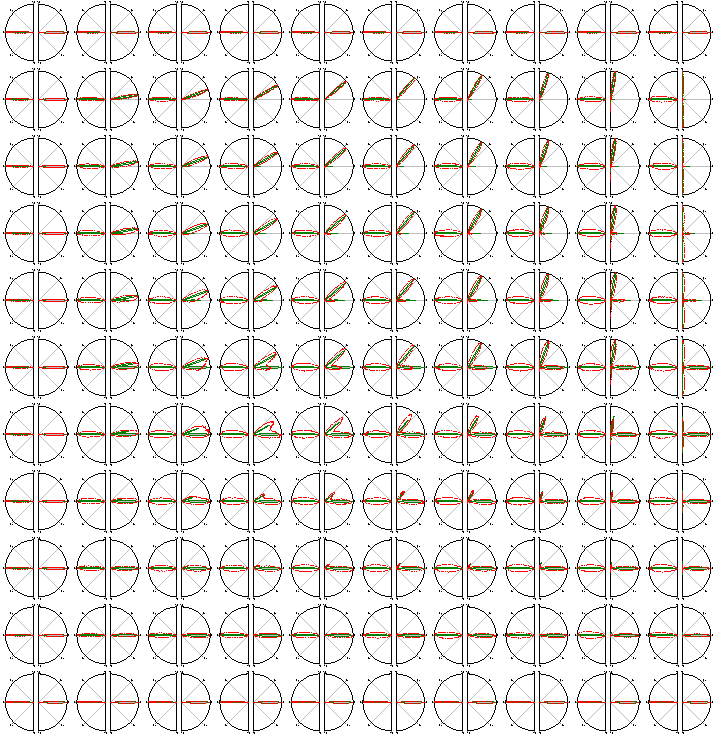
\includegraphics[width=1.0\textwidth]{gfx/model/results/model_analysis.pdf}};
% \begin{scope}[overlay]
%     \draw[->,thick] ($(image.north west)-(0.25,-0.25)$) -- ++(1,0) node [midway, above] {$\Omega$};
%     \draw[->,thick] ($(image.north west)-(0.25,-0.25)$) -- ++(0,-1) node [midway, above, rotate=90] {$\Psi$};
% \end{scope}
% \path ($(image.north west) + (-.5,.5)$) -- ($(image.north east) + (.5,.5)$);
% \end{tikzpicture}
% }
% \caption{model init vs solved}
% \label{app:model_histogram}
% \end{figure}
% %
% \begin{figure}[!tb]
% \centering
% \resizebox{1.0\textwidth}{!}{
% \begin{tikzpicture}[>=latex]
% \node[inner sep=0pt] (image) at (0,0)
%     {\includegraphics[width=1.0\textwidth]{gfx/model/results/histogram.pdf}};
% \begin{scope}[overlay]
%     \draw[->,thick] ($(image.north west)-(0.25,-0.25)$) -- ++(1,0) node [midway, above] {$\Omega$};
%     \draw[->,thick] ($(image.north west)-(0.25,-0.25)$) -- ++(0,-1) node [midway, above, rotate=90] {$\Psi$};
% \end{scope}
% \path ($(image.north west) + (-.5,.5)$) -- ($(image.north east) + (.5,.5)$);
% \end{tikzpicture}
% }
% \caption{Histogram cube\_2pop\_model}
% \label{app:model_histogram}
% \end{figure}
% %
% %
% \begin{figure}[!tb]
% \centering
% \resizebox{1.0\textwidth}{!}{
% \begin{tikzpicture}[>=latex]
% \node[inner sep=0pt] (image) at (0,0)
%     {\includegraphics[width=1.0\textwidth]{gfx/model/results/voxel_size_simulation_analysis.pdf}};
% \begin{scope}[overlay]
%     \draw[->,thick] ($(image.north west)-(0.25,-0.25)$) -- ++(1,0) node [midway, above] {$voxel_size$};
%     \draw[->,thick] ($(image.north west)-(0.25,-0.25)$) -- ++(0,-1) node [midway, above, rotate=90] {$f0_inc$};
% \end{scope}
% \path ($(image.north west) + (-.5,.5)$) -- ($(image.north east) + (.5,.5)$);
% \end{tikzpicture}
% }
% \vspace{-1ex}
% \begin{center}
% \begin{tikzpicture}
%     \draw[thin] (-3.0,-0.625) rectangle (3.0,0.25);
%     \draw [green!50!black] (-2.5,0) -- (-1.5,0) node [below, midway, black] {truth};
%     \draw [red,dashed] (-0.5,0) -- (0.5,0) node [below, midway, black] {model=r};
%     \draw [blue, dash dot] (1.5,0) -- (2.5,0) node [below, midway, black] {model=p};
% \end{tikzpicture}
% \end{center}
% \caption{voxel\_size\_5\_}
% \label{app:model_histogram}
% \end{figure}
% %
% \begin{figure}[!tb]
% \centering
% \resizebox{1.0\textwidth}{!}{
% \begin{tikzpicture}[>=latex]
% \node[inner sep=0pt] (image) at (0,0)
%     {\includegraphics[width=1.0\textwidth]{gfx/simpli/results/simulation_analysis_spheres_LAP_p.pdf}};
% \begin{scope}[overlay]
%     \draw[->,thick] ($(image.north west)-(0.25,-0.25)$) -- ++(1,0) node [midway, above] {$\mathfrak{f}_0^\alpha$};
%     \draw[->,thick] ($(image.north west)-(0.25,-0.25)$) -- ++(0,-1) node [midway, above, rotate=90] {$\mathfrak{f}_0^\Psi$};
% \end{scope}
% \path ($(image.north west) + (-.5,.5)$) -- ($(image.north east) + (.5,.5)$);
% \end{tikzpicture}
% }
% \caption{Sphere LAP p}
% \label{app:model_histogram}
% \end{figure}
% %
% \begin{figure}[!tb]
% \centering
% \resizebox{1.0\textwidth}{!}{
% \begin{tikzpicture}[>=latex]
% \node[inner sep=0pt] (image) at (0,0)
%     {\includegraphics[width=1.0\textwidth]{gfx/simpli/results/simulation_analysis_spheres_LAP_r.pdf}};
% \begin{scope}[overlay]
%     \draw[->,thick] (image.north west) -- ++(1,0) node [midway, above] {$\alpha_0$};
%     \draw[->,thick] (image.north west) -- ++(0,-1) node [midway, above, rotate=90] {$\Psi_0$};
% \end{scope}
% \path ($(image.north west) + (-.5,.5)$) -- ($(image.north east) + (.5,.5)$);
% \end{tikzpicture}
% }
% \caption{Sphere LAP r}
% \label{app:model_histogram}
% \end{figure}
% %
% \begin{figure}[!tb]
% \centering
% \resizebox{1.0\textwidth}{!}{
% \begin{tikzpicture}[>=latex]
% \node[inner sep=0pt] (image) at (0,0)
%     {\includegraphics[width=1.0\textwidth]{gfx/simpli/results/simulation_analysis_spheres_PM_p.pdf}};
% \begin{scope}[overlay]
%     \draw[->,thick] ($(image.north west)-(0.25,-0.25)$) -- ++(1,0) node [midway, above] {$f_0$};
%     \draw[->,thick] ($(image.north west)-(0.25,-0.25)$) -- ++(0,-1) node [midway, above, rotate=90] {$\Psi$};
% \end{scope}
% \path ($(image.north west) + (-.5,.5)$) -- ($(image.north east) + (.5,.5)$);
% \end{tikzpicture}
% }
% \caption{Sphere PM p}
% \label{app:model_histogram}
% \end{figure}
% %
% \begin{figure}[!tb]
% \centering
% \resizebox{1.0\textwidth}{!}{
% \begin{tikzpicture}[>=latex]
% \node[inner sep=0pt] (image) at (0,0)
%     {\includegraphics[width=1.0\textwidth]{gfx/simpli/results/simulation_analysis_spheres_PM_r.pdf}};
% \begin{scope}[overlay]
%     \draw[->,thick] ($(image.north west)-(0.25,-0.25)$) -- ++(1,0) node [midway, above] {$f_0$};
%     \draw[->,thick] ($(image.north west)-(0.25,-0.25)$) -- ++(0,-1) node [midway, above, rotate=90] {$\Psi$};
% \end{scope}
% \path ($(image.north west) + (-.5,.5)$) -- ($(image.north east) + (.5,.5)$);
% \end{tikzpicture}
% }
% \caption{Sphere PM r}
% \label{app:model_histogram}
% \end{figure}
% %
% \begin{figure}[!t]
% \centering
% \resizebox{1.0\textwidth}{!}{
% \includegraphics[width=\textwidth, page=2]{dev/rc1/cube_2pop_orientation_hist2d_output_cube_2pop_135_rc1.pdf}
% }
% \caption[Model orientation histograms]{density distribution of fiber segment orientation in initial and resulting models for $\fiberRadius = \SI{1}{\micro\meter}$. \itodo{fit ESAG} \ITODO{these are only resulting models!}}
% \label{app:modelOrientation}
% \end{figure}
% %
% %
%
\chapter{} % Model analysis
\label{app:modelAnalysis}
%
%
\fakesection{Model parameter}
%
\begin{figure}[!h]
    \centering
    \includegraphics[width=1\textwidth]{dev/rc1/mpara/pre_stats_box_plot_volume_output_parameter_statistic_rc1.pdf}
    \caption{Caption}
    \label{app:appModelVolumeBoxPlot}
\end{figure}
%
% % \foreach \n in {1,3,...,10}{
% % \begin{landscape}
% \begin{figure}[!t]
% \centering
% % \resizebox{\textwidth}{!}{
% \includegraphics[width=\textwidth,page=1]{dev/rc1/mpara/pre_stats_time_evolve_all_output_parameter_statistic_rc1.pdf}
% \includegraphics[width=\textwidth,page=2]{dev/rc1/mpara/pre_stats_time_evolve_all_output_parameter_statistic_rc1.pdf}
% \end{figure}
% % \end{landscape}
%
%
\fakesection{Time evolution}
%
\setlength{\tikzwidth}{\textwidth}
\begin{sidewaysfigure}[]
\centering
\includegraphics[height=\tikzwidth,page=1]{dev/rc1/mpara/pre_stats_time_evolve_all_output_parameter_statistic_rc1.pdf}
\includegraphics[height=\tikzwidth,page=2]{dev/rc1/mpara/pre_stats_time_evolve_all_output_parameter_statistic_rc1.pdf}
\label{app:pste1}
\end{sidewaysfigure}
%
\begin{sidewaysfigure}[]
\centering
% \resizebox{\tikzwidth}{!}{
\includegraphics[height=\tikzwidth,page=3]{dev/rc1/mpara/pre_stats_time_evolve_all_output_parameter_statistic_rc1.pdf}
\includegraphics[height=\tikzwidth,page=4]{dev/rc1/mpara/pre_stats_time_evolve_all_output_parameter_statistic_rc1.pdf}
% }
\label{app:pste2}
\end{sidewaysfigure}
%
\begin{sidewaysfigure}[]
\centering
% \resizebox{\textwidth}{!}{
\includegraphics[height=\tikzwidth,page=5]{dev/rc1/mpara/pre_stats_time_evolve_all_output_parameter_statistic_rc1.pdf}
\includegraphics[height=\tikzwidth,page=6]{dev/rc1/mpara/pre_stats_time_evolve_all_output_parameter_statistic_rc1.pdf}
\label{app:pste3}
\end{sidewaysfigure}
%
\begin{sidewaysfigure}[]
\centering
% \resizebox{\textwidth}{!}{
\includegraphics[height=\tikzwidth,page=7]{dev/rc1/mpara/pre_stats_time_evolve_all_output_parameter_statistic_rc1.pdf}
\includegraphics[height=\tikzwidth,page=8]{dev/rc1/mpara/pre_stats_time_evolve_all_output_parameter_statistic_rc1.pdf}
\label{app:pste4}
\end{sidewaysfigure}
%
\begin{sidewaysfigure}[]
\centering
% \resizebox{\textwidth}{!}{
\includegraphics[height=\tikzwidth,page=9]{dev/rc1/mpara/pre_stats_time_evolve_all_output_parameter_statistic_rc1.pdf}
\includegraphics[height=\tikzwidth,page=10]{dev/rc1/mpara/pre_stats_time_evolve_all_output_parameter_statistic_rc1.pdf}
\label{app:pste5}
\end{sidewaysfigure}
%
%
\fakesection{Histogramms}
%
\begin{figure}
    \centering
    \includegraphics[width=\textwidth, page=2]{dev/rc1/cube_2pop_orientation_hist2d_output_cube_2pop_135_rc1.pdf}
    \caption{Caption}
    \label{app:modelHistOrientation}
\end{figure}[]
%
\fakesection{Speedup}
%
\begin{figure}[!t]
\centering
\includegraphics[page=2]{dev/rc1/speed/boxplot_output_r_0.5__.pkl_speedup.csv.pdf}
\caption[\code{model.Sovler} speedup]{\code{model.Sovler} speedup. The time measurements are taken after $\Delta_{\mathit{steps}}$ for the next $\SI{25}{\steps}$ for parallel $(||)$ and crossing $(\times)$ fiber configurations.}
\label{app:solverSpeedupAll}
\end{figure}
%
%
%
\fakesection{Simulation Library}
\begin{table}[htb]
\centering
\caption[Opening angle distribution]{Orientation statistic of simulation model library.}
\resizebox{\textwidth}{!}{
\pgfplotstabletypeset[%
    thesisTableStyle,
    columns={omega,psi,pop,incl_mean,incl_std,incl_25,incl_50,incl_75,phi_mean,phi_std,phi_25,phi_50,phi_75,mean,std,25,50,75},
    every head row/.style={
        before row={
            \toprule
        },
        after row={$\si{\degree}$ & & & $\si{\degree}$ & $\si{\degree}$ & $\si{\degree}$ & $\si{\degree}$ & $\si{\degree}$ & $\si{\degree}$ & $\si{\degree}$ & $\si{\degree}$ & $\si{\degree}$ & $\si{\degree}$ & $\si{\degree}$ & $\si{\degree}$ & $\si{\degree}$ & $\si{\degree}$ & $\si{\degree}$ \\ \midrule},
    },
    columns/omega/.style={column name=$\Omega$},
    columns/psi/.style={column name=$\Psi$},
    columns/mean/.style={column name=$<d\Omega>$,zerofill,precision=0},
    columns/std/.style={column name=$\sigma(d\Omega)$,zerofill,precision=0},
    columns/25/.style={column name=$25(d\Omega)$,zerofill,precision=0},
    columns/50/.style={column name=$50(d\Omega)$,zerofill,precision=0},
    columns/75/.style={column name=$75(d\Omega)$,zerofill,precision=0},
    columns/incl_mean/.style={column name=$<\alpha>$,fixed,fixed zerofill,precision=0},
    columns/incl_std/.style={column name=$\sigma(\alpha)$,fixed,fixed zerofill,precision=0},
    columns/incl_25/.style={column name=$25(\alpha)$,fixed,fixed zerofill,precision=0},
    columns/incl_50/.style={column name=$50(\alpha)$,fixed,fixed zerofill,precision=0},
    columns/incl_75/.style={column name=$75(\alpha)$,fixed,fixed zerofill,precision=0},
    columns/phi_mean/.style={column name=$<\varphi>$,fixed,fixed zerofill,precision=0},
    columns/phi_std/.style={column name=$\sigma(\varphi)$,fixed,fixed zerofill,precision=0},
    columns/phi_25/.style={column name=$25(\varphi)$,fixed,fixed zerofill,precision=0},
    columns/phi_50/.style={column name=$50(\varphi)$,fixed,fixed zerofill,precision=0},
    columns/phi_75/.style={column name=$75(\varphi)$,fixed,fixed zerofill,precision=0},
    col sep=comma,
    %
]
{dev/rc1/domega/omegas_ms_2pop.csv}
}
\label{app:modelDistribution}
\end{table}
%
% 
%
\chapter{}
\label{app:Simulation}
%
\fakesection{Tissue}
%
\begin{sidewaysfigure}[!p]
\resizebox{\textheight}{!}{
\begin{tabular}{cc}
\includegraphics[]{dev/rc1/tissue/bf_rc1_retardation_PM_Roden.pdf}&
\includegraphics[]{dev/rc1/tissue/bf_rc1_retardation_PM_Human.pdf}\\
\includegraphics[]{dev/rc1/tissue/bf_rc1_transmittance_PM_Roden.pdf}&
\includegraphics[]{dev/rc1/tissue/bf_rc1_transmittance_PM_Human.pdf}
\end{tabular}}
\end{sidewaysfigure}
%
\fakesection{Voxelsize}
%
\begin{figure}[!p]
% 2_simulation/0_parameter/fiber_radii.py
\centering
\includegraphics[width=\textwidth, page=1]{dev/rc1/voxel_size/voxel_size_plots_data_output_vs_135_0.01_6_25_vervet_r_rc1.pdf}
\caption[voxel size model with noise]{The mean difference is constant for smaller voxel sizes and does not start to grow significantly before $\voxels=\SI{0.125}{\micro\meter}$.}
\label{app:voxelsizeNoise}
\end{figure}
%
%
%
\fakesection{domega}
%
\begin{figure}[!t]
    \centering
    \includegraphics[]{dev/rc1/domega/cube_2pop_domega_analysis_all_output.pdf}
    \caption{Direction and inclination distribution of simulation model library.}
    % \label{fig:my_label}
\end{figure}
%
%
%
% %%%%%%%%%%%%%%%%%%%%%%%%%%%%%%%%%%%%%%%%%%%%%%%%%%%%%%%%%%%
% SINGLE
% %%%%%%%%%%%%%%%%%%%%%%%%%%%%%%%%%%%%%%%%%%%%%%%%%%%%%%%%%%%
%
\fakesection{Single fiber population}
%
\begin{figure}[!p]
\centering
% \begin{minipage}{0.45\textwidth}
\resizebox{\textwidth}{!}{
\rotatebox{90}{
\begin{tabular}{c|c}
\begin{tabular}{c|c}
    \includegraphics[]{dev/rc1/single/cube_2pop_135_rc1_single_plots_single_pop_hist_0.0.pdf} &
    \includegraphics[]{dev/rc1/single/cube_2pop_135_rc1_single_plots_single_pop_hist_25.0.pdf} \\
    \includegraphics[]{dev/rc1/single/cube_2pop_135_rc1_single_plots_single_pop_hist_5.0.pdf} &
    \includegraphics[]{dev/rc1/single/cube_2pop_135_rc1_single_plots_single_pop_hist_30.0.pdf} \\
    \includegraphics[]{dev/rc1/single/cube_2pop_135_rc1_single_plots_single_pop_hist_10.0.pdf} &
    \includegraphics[]{dev/rc1/single/cube_2pop_135_rc1_single_plots_single_pop_hist_35.0.pdf} \\
    \includegraphics[]{dev/rc1/single/cube_2pop_135_rc1_single_plots_single_pop_hist_15.0.pdf} &
    \includegraphics[]{dev/rc1/single/cube_2pop_135_rc1_single_plots_single_pop_hist_40.0.pdf} \\
    \includegraphics[]{dev/rc1/single/cube_2pop_135_rc1_single_plots_single_pop_hist_20.0.pdf} &
    \includegraphics[]{dev/rc1/single/cube_2pop_135_rc1_single_plots_single_pop_hist_45.0.pdf}
\end{tabular}
&
\begin{tabular}{c|c}
    \includegraphics[]{dev/rc1/single/cube_2pop_135_rc1_single_plots_single_pop_hist_50.0.pdf} &
    \includegraphics[]{dev/rc1/single/cube_2pop_135_rc1_single_plots_single_pop_hist_75.0.pdf} \\
    \includegraphics[]{dev/rc1/single/cube_2pop_135_rc1_single_plots_single_pop_hist_55.0.pdf} &
    \includegraphics[]{dev/rc1/single/cube_2pop_135_rc1_single_plots_single_pop_hist_80.0.pdf} \\
    \includegraphics[]{dev/rc1/single/cube_2pop_135_rc1_single_plots_single_pop_hist_60.0.pdf} &
    \includegraphics[]{dev/rc1/single/cube_2pop_135_rc1_single_plots_single_pop_hist_85.0.pdf} \\
    \includegraphics[]{dev/rc1/single/cube_2pop_135_rc1_single_plots_single_pop_hist_65.0.pdf} &
    \includegraphics[]{dev/rc1/single/cube_2pop_135_rc1_single_plots_single_pop_hist_90.0.pdf} \\
    \includegraphics[]{dev/rc1/single/cube_2pop_135_rc1_single_plots_single_pop_hist_70.0.pdf} &
\end{tabular}
\end{tabular}
}}
%
\caption[sim]{left: 2d log histogramm orientation from rofl analysis of simulation, right: 2d log histogramm of orientation of model segemnts. \itodo{rfc plots}}
\label{app:single_fiber_pop_hist_app}
\end{figure}
%
%
% %%%%%%%%%%%%%%%%%%%%%%%%%%%%%%%%%%%%%%%%%%%%%%%%%%%%%%%%%%%
% FLAT
% %%%%%%%%%%%%%%%%%%%%%%%%%%%%%%%%%%%%%%%%%%%%%%%%%%%%%%%%%%%
%
\fakesection{Crossing fiber population}
%
\begin{figure}[!p]
\centering
\setlength{\tikzwidth}{0.45\textwidth}
\begin{tabular}{c|c}
    \includegraphics[width=\tikzwidth]{dev/rc1/flat/cube_2pop_135_rc1_flat_plots_flat_pop_hist_omega_0.0_psi_0.3.pdf} &
    \includegraphics[width=\tikzwidth]{dev/rc1/flat/cube_2pop_135_rc1_flat_plots_flat_pop_hist_omega_50.0_psi_0.3.pdf} \\
    \includegraphics[width=\tikzwidth]{dev/rc1/flat/cube_2pop_135_rc1_flat_plots_flat_pop_hist_omega_10.0_psi_0.3.pdf} &
    \includegraphics[width=\tikzwidth]{dev/rc1/flat/cube_2pop_135_rc1_flat_plots_flat_pop_hist_omega_60.0_psi_0.3.pdf} \\
    \includegraphics[width=\tikzwidth]{dev/rc1/flat/cube_2pop_135_rc1_flat_plots_flat_pop_hist_omega_20.0_psi_0.3.pdf} &
    \includegraphics[width=\tikzwidth]{dev/rc1/flat/cube_2pop_135_rc1_flat_plots_flat_pop_hist_omega_70.0_psi_0.3.pdf} \\
    \includegraphics[width=\tikzwidth]{dev/rc1/flat/cube_2pop_135_rc1_flat_plots_flat_pop_hist_omega_30.0_psi_0.3.pdf} &
    \includegraphics[width=\tikzwidth]{dev/rc1/flat/cube_2pop_135_rc1_flat_plots_flat_pop_hist_omega_80.0_psi_0.3.pdf} \\
    \includegraphics[width=\tikzwidth]{dev/rc1/flat/cube_2pop_135_rc1_flat_plots_flat_pop_hist_omega_40.0_psi_0.3.pdf} &
    \includegraphics[width=\tikzwidth]{dev/rc1/flat/cube_2pop_135_rc1_flat_plots_flat_pop_hist_omega_90.0_psi_0.3.pdf}
\end{tabular}
%
\caption[sim]{psi=0.3; left: 2d log histogramm orientation from rofl analysis of simulation, right: 2d log histogram of orientation of model segemnts. \itodo{legende}}
\label{app:flat_03_fiber_pop_hist}
\end{figure}
%
%
%
%
\begin{figure}[!p]
\centering
\setlength{\tikzwidth}{0.45\textwidth}
\begin{tabular}{c|c}
    \includegraphics[width=\tikzwidth]{dev/rc1/flat/cube_2pop_135_rc1_flat_plots_flat_pop_hist_omega_0.0_psi_0.5.pdf} &
    \includegraphics[width=\tikzwidth]{dev/rc1/flat/cube_2pop_135_rc1_flat_plots_flat_pop_hist_omega_50.0_psi_0.5.pdf} \\
    \includegraphics[width=\tikzwidth]{dev/rc1/flat/cube_2pop_135_rc1_flat_plots_flat_pop_hist_omega_10.0_psi_0.5.pdf} &
    \includegraphics[width=\tikzwidth]{dev/rc1/flat/cube_2pop_135_rc1_flat_plots_flat_pop_hist_omega_60.0_psi_0.5.pdf} \\
    \includegraphics[width=\tikzwidth]{dev/rc1/flat/cube_2pop_135_rc1_flat_plots_flat_pop_hist_omega_20.0_psi_0.5.pdf} &
    \includegraphics[width=\tikzwidth]{dev/rc1/flat/cube_2pop_135_rc1_flat_plots_flat_pop_hist_omega_70.0_psi_0.5.pdf} \\
    \includegraphics[width=\tikzwidth]{dev/rc1/flat/cube_2pop_135_rc1_flat_plots_flat_pop_hist_omega_30.0_psi_0.5.pdf} &
    \includegraphics[width=\tikzwidth]{dev/rc1/flat/cube_2pop_135_rc1_flat_plots_flat_pop_hist_omega_80.0_psi_0.5.pdf} \\
    \includegraphics[width=\tikzwidth]{dev/rc1/flat/cube_2pop_135_rc1_flat_plots_flat_pop_hist_omega_40.0_psi_0.5.pdf} &
    \includegraphics[width=\tikzwidth]{dev/rc1/flat/cube_2pop_135_rc1_flat_plots_flat_pop_hist_omega_90.0_psi_0.5.pdf}
\end{tabular}
%
\caption[sim]{psi=0.5; left: 2d log histogramm orientation from rofl analysis of simulation, right: 2d log histogramm of orientation of model segemnts. \itodo{legende}}
\label{app:flat_05_fiber_pop_hist}
\end{figure}
%
%
%
\begin{figure}[!p]
\centering
\resizebox{\textwidth}{!}{
\begin{tabular}{cc}
\includegraphics[page=1]{dev/rc1/analysis/plots_flat_pop_output_cube_2pop_135_rc1_flat.pdf} &
\includegraphics[page=2]{dev/rc1/analysis/plots_flat_pop_output_cube_2pop_135_rc1_flat.pdf}\\
\includegraphics[page=3]{dev/rc1/analysis/plots_flat_pop_output_cube_2pop_135_rc1_flat.pdf} &
\includegraphics[page=4]{dev/rc1/analysis/plots_flat_pop_output_cube_2pop_135_rc1_flat.pdf}
\end{tabular}
}
\end{figure}
%
\begin{figure}[!p]
\centering
\resizebox{\textwidth}{!}{
\begin{tabular}{cc}
\includegraphics[page=5]{dev/rc1/analysis/plots_flat_pop_output_cube_2pop_135_rc1_flat.pdf} &
\includegraphics[page=6]{dev/rc1/analysis/plots_flat_pop_output_cube_2pop_135_rc1_flat.pdf}\\
\includegraphics[page=7]{dev/rc1/analysis/plots_flat_pop_output_cube_2pop_135_rc1_flat.pdf} &
\includegraphics[page=8]{dev/rc1/analysis/plots_flat_pop_output_cube_2pop_135_rc1_flat.pdf}
\end{tabular}
}
\end{figure}
%
\begin{figure}[]
\centering
\resizebox{\textwidth}{!}{
\begin{tabular}{cc}
\includegraphics[page=9]{dev/rc1/analysis/plots_flat_pop_output_cube_2pop_135_rc1_flat.pdf} &
\includegraphics[page=10]{dev/rc1/analysis/plots_flat_pop_output_cube_2pop_135_rc1_flat.pdf}
\end{tabular}
}
\end{figure}
%
%
% %%%%%%%%%%%%%%%%%%%%%%%%%%%%%%%%%%%%%%%%%%%%%%%%%%%%%%%%%%%
% INCLINED
% %%%%%%%%%%%%%%%%%%%%%%%%%%%%%%%%%%%%%%%%%%%%%%%%%%%%%%%%%%%
%
\fakesection{Inclined fiber population}
%
\begin{figure}[!p]
\centering
\setlength{\tikzwidth}{0.45\textwidth}
\begin{tabular}{c|c}
    \includegraphics[width=\tikzwidth]{dev/rc1/inclined/cube_2pop_135_rc1_inclined_plots_inclined_pop_hist_omega_0.0_psi_0.3.pdf} &
    \includegraphics[width=\tikzwidth]{dev/rc1/inclined/cube_2pop_135_rc1_inclined_plots_inclined_pop_hist_omega_50.0_psi_0.3.pdf} \\ \includegraphics[width=\tikzwidth]{dev/rc1/inclined/cube_2pop_135_rc1_inclined_plots_inclined_pop_hist_omega_10.0_psi_0.3.pdf} & \includegraphics[width=\tikzwidth]{dev/rc1/inclined/cube_2pop_135_rc1_inclined_plots_inclined_pop_hist_omega_60.0_psi_0.3.pdf} \\
    \includegraphics[width=\tikzwidth]{dev/rc1/inclined/cube_2pop_135_rc1_inclined_plots_inclined_pop_hist_omega_20.0_psi_0.3.pdf} &
    \includegraphics[width=\tikzwidth]{dev/rc1/inclined/cube_2pop_135_rc1_inclined_plots_inclined_pop_hist_omega_70.0_psi_0.3.pdf} \\ \includegraphics[width=\tikzwidth]{dev/rc1/inclined/cube_2pop_135_rc1_inclined_plots_inclined_pop_hist_omega_30.0_psi_0.3.pdf} & \includegraphics[width=\tikzwidth]{dev/rc1/inclined/cube_2pop_135_rc1_inclined_plots_inclined_pop_hist_omega_80.0_psi_0.3.pdf} \\
    \includegraphics[width=\tikzwidth]{dev/rc1/inclined/cube_2pop_135_rc1_inclined_plots_inclined_pop_hist_omega_40.0_psi_0.3.pdf} &
    \includegraphics[width=\tikzwidth]{dev/rc1/inclined/cube_2pop_135_rc1_inclined_plots_inclined_pop_hist_omega_90.0_psi_0.3.pdf}
\end{tabular}
%
\caption[sim]{psi=0.3; left: 2d log histogramm orientation from rofl analysis of simulation, right: 2d log histogram of orientation of model segemnts. \itodo{legende}}
\label{app:incl_03_fiber_pop_hist}
\end{figure}
%
%
%
%
\begin{figure}[!p]
\centering
\setlength{\tikzwidth}{0.45\textwidth}
\begin{tabular}{c|c}
    \includegraphics[width=\tikzwidth]{dev/rc1/inclined/cube_2pop_135_rc1_inclined_plots_inclined_pop_hist_omega_0.0_psi_0.5.pdf} &
    \includegraphics[width=\tikzwidth]{dev/rc1/inclined/cube_2pop_135_rc1_inclined_plots_inclined_pop_hist_omega_50.0_psi_0.5.pdf} \\
    \includegraphics[width=\tikzwidth]{dev/rc1/inclined/cube_2pop_135_rc1_inclined_plots_inclined_pop_hist_omega_10.0_psi_0.5.pdf} &
    \includegraphics[width=\tikzwidth]{dev/rc1/inclined/cube_2pop_135_rc1_inclined_plots_inclined_pop_hist_omega_60.0_psi_0.5.pdf} \\
    \includegraphics[width=\tikzwidth]{dev/rc1/inclined/cube_2pop_135_rc1_inclined_plots_inclined_pop_hist_omega_20.0_psi_0.5.pdf} &
    \includegraphics[width=\tikzwidth]{dev/rc1/inclined/cube_2pop_135_rc1_inclined_plots_inclined_pop_hist_omega_70.0_psi_0.5.pdf} \\
    \includegraphics[width=\tikzwidth]{dev/rc1/inclined/cube_2pop_135_rc1_inclined_plots_inclined_pop_hist_omega_30.0_psi_0.5.pdf} &
    \includegraphics[width=\tikzwidth]{dev/rc1/inclined/cube_2pop_135_rc1_inclined_plots_inclined_pop_hist_omega_80.0_psi_0.5.pdf} \\
    \includegraphics[width=\tikzwidth]{dev/rc1/inclined/cube_2pop_135_rc1_inclined_plots_inclined_pop_hist_omega_40.0_psi_0.5.pdf} &
    \includegraphics[width=\tikzwidth]{dev/rc1/inclined/cube_2pop_135_rc1_inclined_plots_inclined_pop_hist_omega_90.0_psi_0.5.pdf}
\end{tabular}
%
\caption[sim]{psi=0.5; left: 2d log histogramm orientation from rofl analysis of simulation, right: 2d log histogramm of orientation of model segemnts. \itodo{legende}}
\label{app:incl_05_fiber_pop_hist}
\end{figure}
%
%
%
\begin{figure}[!p]
\centering
\resizebox{\textwidth}{!}{
\begin{tabular}{cc}
\includegraphics[page=1]{dev/rc1/analysis/plots_inclined_pop_output_cube_2pop_135_rc1_inclined.pdf} &
\includegraphics[page=2]{dev/rc1/analysis/plots_inclined_pop_output_cube_2pop_135_rc1_inclined.pdf}\\
\includegraphics[page=3]{dev/rc1/analysis/plots_inclined_pop_output_cube_2pop_135_rc1_inclined.pdf} &
\includegraphics[page=4]{dev/rc1/analysis/plots_inclined_pop_output_cube_2pop_135_rc1_inclined.pdf}
\end{tabular}
}
\end{figure}
%
\begin{figure}[!p]
\centering
\resizebox{\textwidth}{!}{
\begin{tabular}{cc}
\includegraphics[page=5]{dev/rc1/analysis/plots_inclined_pop_output_cube_2pop_135_rc1_inclined.pdf} &
\includegraphics[page=6]{dev/rc1/analysis/plots_inclined_pop_output_cube_2pop_135_rc1_inclined.pdf}\\
\includegraphics[page=7]{dev/rc1/analysis/plots_inclined_pop_output_cube_2pop_135_rc1_inclined.pdf} &
\includegraphics[page=8]{dev/rc1/analysis/plots_inclined_pop_output_cube_2pop_135_rc1_inclined.pdf}
\end{tabular}
}
\end{figure}
%
\begin{figure}[!p]
\centering
\resizebox{\textwidth}{!}{
\begin{tabular}{cc}
\includegraphics[page=9]{dev/rc1/analysis/plots_inclined_pop_output_cube_2pop_135_rc1_inclined.pdf} &
\includegraphics[page=10]{dev/rc1/analysis/plots_inclined_pop_output_cube_2pop_135_rc1_inclined.pdf}
\end{tabular}
}
\end{figure}
%
% %
% %
%
% \newpage
% \mbox{}
%
% **************************************************
% End of Document CONTENT
% **************************************************
\end{document}
